\documentclass[twoside]{book}

% Packages required by doxygen
\usepackage{fixltx2e}
\usepackage{calc}
\usepackage{doxygen}
\usepackage[export]{adjustbox} % also loads graphicx
\usepackage{graphicx}
\usepackage[utf8]{inputenc}
\usepackage{makeidx}
\usepackage{multicol}
\usepackage{multirow}
\PassOptionsToPackage{warn}{textcomp}
\usepackage{textcomp}
\usepackage[nointegrals]{wasysym}
\usepackage[table]{xcolor}

% Font selection
\usepackage[T1]{fontenc}
\usepackage[scaled=.90]{helvet}
\usepackage{courier}
\usepackage{amssymb}
\usepackage{sectsty}
\renewcommand{\familydefault}{\sfdefault}
\allsectionsfont{%
  \fontseries{bc}\selectfont%
  \color{darkgray}%
}
\renewcommand{\DoxyLabelFont}{%
  \fontseries{bc}\selectfont%
  \color{darkgray}%
}
\newcommand{\+}{\discretionary{\mbox{\scriptsize$\hookleftarrow$}}{}{}}

% Page & text layout
\usepackage{geometry}
\geometry{%
  a4paper,%
  top=2.5cm,%
  bottom=2.5cm,%
  left=2.5cm,%
  right=2.5cm%
}
\tolerance=750
\hfuzz=15pt
\hbadness=750
\setlength{\emergencystretch}{15pt}
\setlength{\parindent}{0cm}
\setlength{\parskip}{3ex plus 2ex minus 2ex}
\makeatletter
\renewcommand{\paragraph}{%
  \@startsection{paragraph}{4}{0ex}{-1.0ex}{1.0ex}{%
    \normalfont\normalsize\bfseries\SS@parafont%
  }%
}
\renewcommand{\subparagraph}{%
  \@startsection{subparagraph}{5}{0ex}{-1.0ex}{1.0ex}{%
    \normalfont\normalsize\bfseries\SS@subparafont%
  }%
}
\makeatother

% Headers & footers
\usepackage{fancyhdr}
\pagestyle{fancyplain}
\fancyhead[LE]{\fancyplain{}{\bfseries\thepage}}
\fancyhead[CE]{\fancyplain{}{}}
\fancyhead[RE]{\fancyplain{}{\bfseries\leftmark}}
\fancyhead[LO]{\fancyplain{}{\bfseries\rightmark}}
\fancyhead[CO]{\fancyplain{}{}}
\fancyhead[RO]{\fancyplain{}{\bfseries\thepage}}
\fancyfoot[LE]{\fancyplain{}{}}
\fancyfoot[CE]{\fancyplain{}{}}
\fancyfoot[RE]{\fancyplain{}{\bfseries\scriptsize Generated by Doxygen }}
\fancyfoot[LO]{\fancyplain{}{\bfseries\scriptsize Generated by Doxygen }}
\fancyfoot[CO]{\fancyplain{}{}}
\fancyfoot[RO]{\fancyplain{}{}}
\renewcommand{\footrulewidth}{0.4pt}
\renewcommand{\chaptermark}[1]{%
  \markboth{#1}{}%
}
\renewcommand{\sectionmark}[1]{%
  \markright{\thesection\ #1}%
}

% Indices & bibliography
\usepackage{natbib}
\usepackage[titles]{tocloft}
\setcounter{tocdepth}{3}
\setcounter{secnumdepth}{5}
\makeindex

% Hyperlinks (required, but should be loaded last)
\usepackage{ifpdf}
\ifpdf
  \usepackage[pdftex,pagebackref=true]{hyperref}
\else
  \usepackage[ps2pdf,pagebackref=true]{hyperref}
\fi
\hypersetup{%
  colorlinks=true,%
  linkcolor=blue,%
  citecolor=blue,%
  unicode%
}

% Custom commands
\newcommand{\clearemptydoublepage}{%
  \newpage{\pagestyle{empty}\cleardoublepage}%
}

\usepackage{caption}
\captionsetup{labelsep=space,justification=centering,font={bf},singlelinecheck=off,skip=4pt,position=top}

%===== C O N T E N T S =====

\begin{document}

% Titlepage & ToC
\hypersetup{pageanchor=false,
             bookmarksnumbered=true,
             pdfencoding=unicode
            }
\pagenumbering{alph}
\begin{titlepage}
\vspace*{7cm}
\begin{center}%
{\Large P\+D\+N\+Sim }\\
\vspace*{1cm}
{\large Generated by Doxygen 1.8.13}\\
\end{center}
\end{titlepage}
\clearemptydoublepage
\pagenumbering{roman}
\tableofcontents
\clearemptydoublepage
\pagenumbering{arabic}
\hypersetup{pageanchor=true}

%--- Begin generated contents ---
\chapter{Namespace Index}
\section{Namespace List}
Here is a list of all namespaces with brief descriptions\+:\begin{DoxyCompactList}
\item\contentsline{section}{\hyperlink{namespacesta}{sta} }{\pageref{namespacesta}}{}
\end{DoxyCompactList}

\chapter{Data Structure Index}
\section{Data Structures}
Here are the data structures with brief descriptions\+:\begin{DoxyCompactList}
\item\contentsline{section}{\hyperlink{structCscMatrix}{Csc\+Matrix} \\*Data structure for the Compressed Sparse Column Matrix }{\pageref{structCscMatrix}}{}
\item\contentsline{section}{\hyperlink{structDokMatrix}{Dok\+Matrix} \\*Data structure for the Dictionary of Keys Matrix }{\pageref{structDokMatrix}}{}
\item\contentsline{section}{\hyperlink{classGMat}{G\+Mat} \\*G matrix class }{\pageref{classGMat}}{}
\item\contentsline{section}{\hyperlink{classIRSolver}{I\+R\+Solver} \\*Class for IR solver }{\pageref{classIRSolver}}{}
\item\contentsline{section}{\hyperlink{classNode}{Node} \\*\hyperlink{classNode}{Node} class which stores the properties of the node of the P\+DN }{\pageref{classNode}}{}
\item\contentsline{section}{\hyperlink{classParameters}{Parameters} }{\pageref{classParameters}}{}
\item\contentsline{section}{\hyperlink{classPDNSim}{P\+D\+N\+Sim} }{\pageref{classPDNSim}}{}
\item\contentsline{section}{\hyperlink{classPowerInst}{Power\+Inst} \\*Calculates the power per instance using Open\+S\+TA }{\pageref{classPowerInst}}{}
\item\contentsline{section}{\hyperlink{structswig__attribute}{swig\+\_\+attribute} }{\pageref{structswig__attribute}}{}
\item\contentsline{section}{\hyperlink{structswig__cast__info}{swig\+\_\+cast\+\_\+info} }{\pageref{structswig__cast__info}}{}
\item\contentsline{section}{\hyperlink{structswig__class}{swig\+\_\+class} }{\pageref{structswig__class}}{}
\item\contentsline{section}{\hyperlink{structswig__command__info}{swig\+\_\+command\+\_\+info} }{\pageref{structswig__command__info}}{}
\item\contentsline{section}{\hyperlink{structswig__const__info}{swig\+\_\+const\+\_\+info} }{\pageref{structswig__const__info}}{}
\item\contentsline{section}{\hyperlink{structswig__instance}{swig\+\_\+instance} }{\pageref{structswig__instance}}{}
\item\contentsline{section}{\hyperlink{structswig__method}{swig\+\_\+method} }{\pageref{structswig__method}}{}
\item\contentsline{section}{\hyperlink{structswig__module__info}{swig\+\_\+module\+\_\+info} }{\pageref{structswig__module__info}}{}
\item\contentsline{section}{\hyperlink{structswig__type__info}{swig\+\_\+type\+\_\+info} }{\pageref{structswig__type__info}}{}
\item\contentsline{section}{\hyperlink{structswig__var__info}{swig\+\_\+var\+\_\+info} }{\pageref{structswig__var__info}}{}
\end{DoxyCompactList}

\chapter{File Index}
\section{File List}
Here is a list of all files with brief descriptions\+:\begin{DoxyCompactList}
\item\contentsline{section}{src/\hyperlink{get__power_8cpp}{get\+\_\+power.\+cpp} }{\pageref{get__power_8cpp}}{}
\item\contentsline{section}{src/\hyperlink{get__power_8h}{get\+\_\+power.\+h} }{\pageref{get__power_8h}}{}
\item\contentsline{section}{src/\hyperlink{gmat_8cpp}{gmat.\+cpp} }{\pageref{gmat_8cpp}}{}
\item\contentsline{section}{src/\hyperlink{gmat_8h}{gmat.\+h} }{\pageref{gmat_8h}}{}
\item\contentsline{section}{src/\hyperlink{ir__solver_8cpp}{ir\+\_\+solver.\+cpp} }{\pageref{ir__solver_8cpp}}{}
\item\contentsline{section}{src/\hyperlink{ir__solver_8h}{ir\+\_\+solver.\+h} }{\pageref{ir__solver_8h}}{}
\item\contentsline{section}{src/\hyperlink{main_8cpp}{main.\+cpp} }{\pageref{main_8cpp}}{}
\item\contentsline{section}{src/\hyperlink{node_8cpp}{node.\+cpp} }{\pageref{node_8cpp}}{}
\item\contentsline{section}{src/\hyperlink{node_8h}{node.\+h} }{\pageref{node_8h}}{}
\item\contentsline{section}{src/\hyperlink{parameters_8cpp}{parameters.\+cpp} }{\pageref{parameters_8cpp}}{}
\item\contentsline{section}{src/\hyperlink{parameters_8h}{parameters.\+h} }{\pageref{parameters_8h}}{}
\item\contentsline{section}{src/\hyperlink{pdnsim__external_8cpp}{pdnsim\+\_\+external.\+cpp} }{\pageref{pdnsim__external_8cpp}}{}
\item\contentsline{section}{src/\hyperlink{pdnsim__external_8h}{pdnsim\+\_\+external.\+h} }{\pageref{pdnsim__external_8h}}{}
\item\contentsline{section}{src/\hyperlink{pdnsim__wrap_8cpp}{pdnsim\+\_\+wrap.\+cpp} }{\pageref{pdnsim__wrap_8cpp}}{}
\end{DoxyCompactList}

\chapter{Namespace Documentation}
\hypertarget{namespacesta}{}\section{sta Namespace Reference}
\label{namespacesta}\index{sta@{sta}}
\subsection*{Variables}
\begin{DoxyCompactItemize}
\item 
const char $\ast$ \hyperlink{namespacesta_a25423e815a38020350ff9ec056668087}{tcl\+\_\+inits} \mbox{[}$\,$\mbox{]}
\end{DoxyCompactItemize}


\subsection{Variable Documentation}
\mbox{\Hypertarget{namespacesta_a25423e815a38020350ff9ec056668087}\label{namespacesta_a25423e815a38020350ff9ec056668087}} 
\index{sta@{sta}!tcl\+\_\+inits@{tcl\+\_\+inits}}
\index{tcl\+\_\+inits@{tcl\+\_\+inits}!sta@{sta}}
\subsubsection{\texorpdfstring{tcl\+\_\+inits}{tcl\_inits}}
{\footnotesize\ttfamily const char$\ast$ sta\+::tcl\+\_\+inits\mbox{[}$\,$\mbox{]}}


\chapter{Data Structure Documentation}
\hypertarget{structCscMatrix}{}\section{Csc\+Matrix Struct Reference}
\label{structCscMatrix}\index{Csc\+Matrix@{Csc\+Matrix}}


Data structure for the Compressed Sparse Column Matrix.  




{\ttfamily \#include $<$node.\+h$>$}

\subsection*{Data Fields}
\begin{DoxyCompactItemize}
\item 
\hyperlink{node_8h_a5b622fe4354316a2f349615d150ae998}{Node\+Idx} \hyperlink{structCscMatrix_a9e6fea3106af21e3c05e1c497e0ee69f}{num\+\_\+rows}
\item 
\hyperlink{node_8h_a5b622fe4354316a2f349615d150ae998}{Node\+Idx} \hyperlink{structCscMatrix_add293b1d06d14359190fc4cb3fd35714}{num\+\_\+cols}
\item 
\hyperlink{node_8h_a5b622fe4354316a2f349615d150ae998}{Node\+Idx} \hyperlink{structCscMatrix_ae5f18924a98bd8115bd34bb5a61bf1c1}{nnz}
\item 
std\+::vector$<$ \hyperlink{node_8h_a5b622fe4354316a2f349615d150ae998}{Node\+Idx} $>$ \hyperlink{structCscMatrix_a2eef34de7f3687351e18cb8e1da74329}{row\+\_\+idx}
\item 
std\+::vector$<$ \hyperlink{node_8h_a5b622fe4354316a2f349615d150ae998}{Node\+Idx} $>$ \hyperlink{structCscMatrix_a6bd9ad7395e2e10ee4bb0cf9c1e1ddc9}{col\+\_\+ptr}
\item 
std\+::vector$<$ double $>$ \hyperlink{structCscMatrix_ae540c6a54027394970614fe75f20d68a}{values}
\end{DoxyCompactItemize}


\subsection{Detailed Description}
Data structure for the Compressed Sparse Column Matrix. 

\subsection{Field Documentation}
\mbox{\Hypertarget{structCscMatrix_a6bd9ad7395e2e10ee4bb0cf9c1e1ddc9}\label{structCscMatrix_a6bd9ad7395e2e10ee4bb0cf9c1e1ddc9}} 
\index{Csc\+Matrix@{Csc\+Matrix}!col\+\_\+ptr@{col\+\_\+ptr}}
\index{col\+\_\+ptr@{col\+\_\+ptr}!Csc\+Matrix@{Csc\+Matrix}}
\subsubsection{\texorpdfstring{col\+\_\+ptr}{col\_ptr}}
{\footnotesize\ttfamily std\+::vector$<$\hyperlink{node_8h_a5b622fe4354316a2f349615d150ae998}{Node\+Idx}$>$ Csc\+Matrix\+::col\+\_\+ptr}

\mbox{\Hypertarget{structCscMatrix_ae5f18924a98bd8115bd34bb5a61bf1c1}\label{structCscMatrix_ae5f18924a98bd8115bd34bb5a61bf1c1}} 
\index{Csc\+Matrix@{Csc\+Matrix}!nnz@{nnz}}
\index{nnz@{nnz}!Csc\+Matrix@{Csc\+Matrix}}
\subsubsection{\texorpdfstring{nnz}{nnz}}
{\footnotesize\ttfamily \hyperlink{node_8h_a5b622fe4354316a2f349615d150ae998}{Node\+Idx} Csc\+Matrix\+::nnz}

\mbox{\Hypertarget{structCscMatrix_add293b1d06d14359190fc4cb3fd35714}\label{structCscMatrix_add293b1d06d14359190fc4cb3fd35714}} 
\index{Csc\+Matrix@{Csc\+Matrix}!num\+\_\+cols@{num\+\_\+cols}}
\index{num\+\_\+cols@{num\+\_\+cols}!Csc\+Matrix@{Csc\+Matrix}}
\subsubsection{\texorpdfstring{num\+\_\+cols}{num\_cols}}
{\footnotesize\ttfamily \hyperlink{node_8h_a5b622fe4354316a2f349615d150ae998}{Node\+Idx} Csc\+Matrix\+::num\+\_\+cols}

\mbox{\Hypertarget{structCscMatrix_a9e6fea3106af21e3c05e1c497e0ee69f}\label{structCscMatrix_a9e6fea3106af21e3c05e1c497e0ee69f}} 
\index{Csc\+Matrix@{Csc\+Matrix}!num\+\_\+rows@{num\+\_\+rows}}
\index{num\+\_\+rows@{num\+\_\+rows}!Csc\+Matrix@{Csc\+Matrix}}
\subsubsection{\texorpdfstring{num\+\_\+rows}{num\_rows}}
{\footnotesize\ttfamily \hyperlink{node_8h_a5b622fe4354316a2f349615d150ae998}{Node\+Idx} Csc\+Matrix\+::num\+\_\+rows}

\mbox{\Hypertarget{structCscMatrix_a2eef34de7f3687351e18cb8e1da74329}\label{structCscMatrix_a2eef34de7f3687351e18cb8e1da74329}} 
\index{Csc\+Matrix@{Csc\+Matrix}!row\+\_\+idx@{row\+\_\+idx}}
\index{row\+\_\+idx@{row\+\_\+idx}!Csc\+Matrix@{Csc\+Matrix}}
\subsubsection{\texorpdfstring{row\+\_\+idx}{row\_idx}}
{\footnotesize\ttfamily std\+::vector$<$\hyperlink{node_8h_a5b622fe4354316a2f349615d150ae998}{Node\+Idx}$>$ Csc\+Matrix\+::row\+\_\+idx}

\mbox{\Hypertarget{structCscMatrix_ae540c6a54027394970614fe75f20d68a}\label{structCscMatrix_ae540c6a54027394970614fe75f20d68a}} 
\index{Csc\+Matrix@{Csc\+Matrix}!values@{values}}
\index{values@{values}!Csc\+Matrix@{Csc\+Matrix}}
\subsubsection{\texorpdfstring{values}{values}}
{\footnotesize\ttfamily std\+::vector$<$double$>$ Csc\+Matrix\+::values}



The documentation for this struct was generated from the following file\+:\begin{DoxyCompactItemize}
\item 
src/\hyperlink{node_8h}{node.\+h}\end{DoxyCompactItemize}

\hypertarget{structDokMatrix}{}\section{Dok\+Matrix Struct Reference}
\label{structDokMatrix}\index{Dok\+Matrix@{Dok\+Matrix}}


Data structure for the Dictionary of Keys Matrix.  




{\ttfamily \#include $<$node.\+h$>$}

\subsection*{Data Fields}
\begin{DoxyCompactItemize}
\item 
\hyperlink{node_8h_a5b622fe4354316a2f349615d150ae998}{Node\+Idx} \hyperlink{structDokMatrix_a653139601f15712d7fea0179d19824a1}{num\+\_\+rows}
\item 
\hyperlink{node_8h_a5b622fe4354316a2f349615d150ae998}{Node\+Idx} \hyperlink{structDokMatrix_a6d86fd874eb6e507f339699bc0764230}{num\+\_\+cols}
\item 
std\+::map$<$ \hyperlink{node_8h_aaffe095b1e5d88040e6ca3976576fccf}{G\+Mat\+Loc}, double $>$ \hyperlink{structDokMatrix_a1474a0133b470ffb7058cc88962046e6}{values}
\end{DoxyCompactItemize}


\subsection{Detailed Description}
Data structure for the Dictionary of Keys Matrix. 

\subsection{Field Documentation}
\mbox{\Hypertarget{structDokMatrix_a6d86fd874eb6e507f339699bc0764230}\label{structDokMatrix_a6d86fd874eb6e507f339699bc0764230}} 
\index{Dok\+Matrix@{Dok\+Matrix}!num\+\_\+cols@{num\+\_\+cols}}
\index{num\+\_\+cols@{num\+\_\+cols}!Dok\+Matrix@{Dok\+Matrix}}
\subsubsection{\texorpdfstring{num\+\_\+cols}{num\_cols}}
{\footnotesize\ttfamily \hyperlink{node_8h_a5b622fe4354316a2f349615d150ae998}{Node\+Idx} Dok\+Matrix\+::num\+\_\+cols}

\mbox{\Hypertarget{structDokMatrix_a653139601f15712d7fea0179d19824a1}\label{structDokMatrix_a653139601f15712d7fea0179d19824a1}} 
\index{Dok\+Matrix@{Dok\+Matrix}!num\+\_\+rows@{num\+\_\+rows}}
\index{num\+\_\+rows@{num\+\_\+rows}!Dok\+Matrix@{Dok\+Matrix}}
\subsubsection{\texorpdfstring{num\+\_\+rows}{num\_rows}}
{\footnotesize\ttfamily \hyperlink{node_8h_a5b622fe4354316a2f349615d150ae998}{Node\+Idx} Dok\+Matrix\+::num\+\_\+rows}

\mbox{\Hypertarget{structDokMatrix_a1474a0133b470ffb7058cc88962046e6}\label{structDokMatrix_a1474a0133b470ffb7058cc88962046e6}} 
\index{Dok\+Matrix@{Dok\+Matrix}!values@{values}}
\index{values@{values}!Dok\+Matrix@{Dok\+Matrix}}
\subsubsection{\texorpdfstring{values}{values}}
{\footnotesize\ttfamily std\+::map$<$\hyperlink{node_8h_aaffe095b1e5d88040e6ca3976576fccf}{G\+Mat\+Loc}, double$>$ Dok\+Matrix\+::values}



The documentation for this struct was generated from the following file\+:\begin{DoxyCompactItemize}
\item 
src/\hyperlink{node_8h}{node.\+h}\end{DoxyCompactItemize}

\hypertarget{classGMat}{}\section{G\+Mat Class Reference}
\label{classGMat}\index{G\+Mat@{G\+Mat}}


G matrix class.  




{\ttfamily \#include $<$gmat.\+h$>$}

\subsection*{Public Member Functions}
\begin{DoxyCompactItemize}
\item 
\hyperlink{classGMat_ad89367522ad38208488689b4146b6bbc}{G\+Mat} (int t\+\_\+num\+\_\+layers, int t\+\_\+num\+C4)
\begin{DoxyCompactList}\small\item\em Constructor for creating the G matrix. \end{DoxyCompactList}\item 
\hyperlink{classGMat_aeb2bc57952d6046f91afac0bcb3a7243}{$\sim$\+G\+Mat} ()
\begin{DoxyCompactList}\small\item\em Destructor of the G matrix. \end{DoxyCompactList}\item 
\hyperlink{classNode}{Node} $\ast$ \hyperlink{classGMat_a48cc4288be2ae357591bab12339e0114}{Get\+Node} (\hyperlink{node_8h_a5b622fe4354316a2f349615d150ae998}{Node\+Idx} t\+\_\+node)
\begin{DoxyCompactList}\small\item\em Function to return a pointer to the node with a index. \end{DoxyCompactList}\item 
\hyperlink{classNode}{Node} $\ast$ \hyperlink{classGMat_a54844be32da6280169a0f8ee08283d5a}{Get\+Node} (int t\+\_\+x, int t\+\_\+y, int t\+\_\+l)
\begin{DoxyCompactList}\small\item\em Function to return a pointer to the node with the x, y, and layer number. \end{DoxyCompactList}\item 
void \hyperlink{classGMat_a96d512b19a257d2361eac59dacee218d}{Set\+Node} (\hyperlink{node_8h_a5b622fe4354316a2f349615d150ae998}{Node\+Idx} t\+\_\+node\+\_\+loc, \hyperlink{classNode}{Node} $\ast$t\+\_\+node)
\begin{DoxyCompactList}\small\item\em Function to set attributes of the node with index and node pointer. \end{DoxyCompactList}\item 
\hyperlink{classNode}{Node} $\ast$ \hyperlink{classGMat_a6edc525006b72ebcd8b9cfbbec60e9ae}{Set\+Node} (int t\+\_\+x, int t\+\_\+y, int t\+\_\+layer, \hyperlink{node_8h_acf0ff4a0bb7e0c9b5900382cbd2aa614}{B\+Box} t\+\_\+b\+Box)
\begin{DoxyCompactList}\small\item\em Function to create a node. \end{DoxyCompactList}\item 
void \hyperlink{classGMat_aab1c09d83c7ad0b0b16d1c8059f1220b}{Insert\+Node} (\hyperlink{classNode}{Node} $\ast$t\+\_\+node)
\begin{DoxyCompactList}\small\item\em Function to insert a node into the matrix. \end{DoxyCompactList}\item 
void \hyperlink{classGMat_a890e83e8d1d373e3858bd213b76c2da9}{Print} ()
\begin{DoxyCompactList}\small\item\em Function that prints the G matrix for debug purposes. \end{DoxyCompactList}\item 
void \hyperlink{classGMat_a1981ec0047b10ef19b2e4734921a5452}{Set\+Conductance} (\hyperlink{classNode}{Node} $\ast$t\+\_\+node1, \hyperlink{classNode}{Node} $\ast$t\+\_\+node2, double t\+\_\+cond)
\begin{DoxyCompactList}\small\item\em Function to add the conductance value between two nodes. \end{DoxyCompactList}\item 
void \hyperlink{classGMat_ab3e602af5a1537611ec1a8bfd798b688}{Initialize\+Gmat\+Dok} ()
\begin{DoxyCompactList}\small\item\em Function to initialize the sparse dok matrix. \end{DoxyCompactList}\item 
\hyperlink{node_8h_a5b622fe4354316a2f349615d150ae998}{Node\+Idx} \hyperlink{classGMat_aa0f8d64bc65172c457d7d1d4a2156b79}{Get\+Num\+Nodes} ()
\begin{DoxyCompactList}\small\item\em Function that returns the number of nodes in the G matrix. \end{DoxyCompactList}\item 
\hyperlink{structCscMatrix}{Csc\+Matrix} $\ast$ \hyperlink{classGMat_a907a945858399a70cc5b77952b81d25a}{Get\+G\+Mat} ()
\begin{DoxyCompactList}\small\item\em Function to return a pointer to the G matrix. \end{DoxyCompactList}\item 
void \hyperlink{classGMat_a0d8697945b060deaaf4bbd3a444aab6f}{Generate\+Stripe\+Conductance} (int t\+\_\+l, odb\+::db\+Tech\+Layer\+Dir\+::\+Value layer\+\_\+dir, int t\+\_\+x\+\_\+min, int t\+\_\+x\+\_\+max, int t\+\_\+y\+\_\+min, int t\+\_\+y\+\_\+max, double t\+\_\+rho)
\begin{DoxyCompactList}\small\item\em Function to get the conductance of the strip of the power grid. \end{DoxyCompactList}\item 
void \hyperlink{classGMat_a21ee1650f436e769255235d3b2fe8aa8}{Add\+C4\+Bump} (int t\+\_\+loc, int t\+\_\+\+C4\+Num)
\begin{DoxyCompactList}\small\item\em Function to add the voltage source based on C4 bump location. \end{DoxyCompactList}\item 
void \hyperlink{classGMat_acc6b68783732ff34b6dd4098cb738836}{Generate\+C\+S\+C\+Matrix} ()
\begin{DoxyCompactList}\small\item\em Function which generates the compressed sparse column matrix. \end{DoxyCompactList}\item 
std\+::vector$<$ \hyperlink{classNode}{Node} $\ast$ $>$ \hyperlink{classGMat_a9bc88ff1d3a55795024e814de8c69617}{Get\+All\+Nodes} ()
\begin{DoxyCompactList}\small\item\em Function to return a vector which contains a pointer to all the nodes. \end{DoxyCompactList}\end{DoxyCompactItemize}


\subsection{Detailed Description}
G matrix class. 

Class to store the G matrix. Contains the member functions for all node related operations. 

\subsection{Constructor \& Destructor Documentation}
\mbox{\Hypertarget{classGMat_ad89367522ad38208488689b4146b6bbc}\label{classGMat_ad89367522ad38208488689b4146b6bbc}} 
\index{G\+Mat@{G\+Mat}!G\+Mat@{G\+Mat}}
\index{G\+Mat@{G\+Mat}!G\+Mat@{G\+Mat}}
\subsubsection{\texorpdfstring{G\+Mat()}{GMat()}}
{\footnotesize\ttfamily G\+Mat\+::\+G\+Mat (\begin{DoxyParamCaption}\item[{int}]{t\+\_\+num\+\_\+layers,  }\item[{int}]{t\+\_\+num\+C4 }\end{DoxyParamCaption})\hspace{0.3cm}{\ttfamily [inline]}}



Constructor for creating the G matrix. 

\mbox{\Hypertarget{classGMat_aeb2bc57952d6046f91afac0bcb3a7243}\label{classGMat_aeb2bc57952d6046f91afac0bcb3a7243}} 
\index{G\+Mat@{G\+Mat}!````~G\+Mat@{$\sim$\+G\+Mat}}
\index{````~G\+Mat@{$\sim$\+G\+Mat}!G\+Mat@{G\+Mat}}
\subsubsection{\texorpdfstring{$\sim$\+G\+Mat()}{~GMat()}}
{\footnotesize\ttfamily G\+Mat\+::$\sim$\+G\+Mat (\begin{DoxyParamCaption}{ }\end{DoxyParamCaption})\hspace{0.3cm}{\ttfamily [inline]}}



Destructor of the G matrix. 



\subsection{Member Function Documentation}
\mbox{\Hypertarget{classGMat_a21ee1650f436e769255235d3b2fe8aa8}\label{classGMat_a21ee1650f436e769255235d3b2fe8aa8}} 
\index{G\+Mat@{G\+Mat}!Add\+C4\+Bump@{Add\+C4\+Bump}}
\index{Add\+C4\+Bump@{Add\+C4\+Bump}!G\+Mat@{G\+Mat}}
\subsubsection{\texorpdfstring{Add\+C4\+Bump()}{AddC4Bump()}}
{\footnotesize\ttfamily void G\+Mat\+::\+Add\+C4\+Bump (\begin{DoxyParamCaption}\item[{int}]{t\+\_\+loc,  }\item[{int}]{t\+\_\+\+C4\+Num }\end{DoxyParamCaption})}



Function to add the voltage source based on C4 bump location. 

Function which add the values in the G matrix for the.

Directly updates the G matrix 
\begin{DoxyParams}{Parameters}
{\em t\+\_\+loc} & Location of the C4 bump \\
\hline
{\em t\+\_\+\+C4\+Num} & C4 bump number \\
\hline
\end{DoxyParams}
\begin{DoxyReturn}{Returns}
nothing 
\end{DoxyReturn}
\mbox{\Hypertarget{classGMat_acc6b68783732ff34b6dd4098cb738836}\label{classGMat_acc6b68783732ff34b6dd4098cb738836}} 
\index{G\+Mat@{G\+Mat}!Generate\+C\+S\+C\+Matrix@{Generate\+C\+S\+C\+Matrix}}
\index{Generate\+C\+S\+C\+Matrix@{Generate\+C\+S\+C\+Matrix}!G\+Mat@{G\+Mat}}
\subsubsection{\texorpdfstring{Generate\+C\+S\+C\+Matrix()}{GenerateCSCMatrix()}}
{\footnotesize\ttfamily void G\+Mat\+::\+Generate\+C\+S\+C\+Matrix (\begin{DoxyParamCaption}{ }\end{DoxyParamCaption})}



Function which generates the compressed sparse column matrix. 

Function which converts the D\+OK matrix into C\+SC format in a sparse method. \mbox{\Hypertarget{classGMat_a0d8697945b060deaaf4bbd3a444aab6f}\label{classGMat_a0d8697945b060deaaf4bbd3a444aab6f}} 
\index{G\+Mat@{G\+Mat}!Generate\+Stripe\+Conductance@{Generate\+Stripe\+Conductance}}
\index{Generate\+Stripe\+Conductance@{Generate\+Stripe\+Conductance}!G\+Mat@{G\+Mat}}
\subsubsection{\texorpdfstring{Generate\+Stripe\+Conductance()}{GenerateStripeConductance()}}
{\footnotesize\ttfamily void G\+Mat\+::\+Generate\+Stripe\+Conductance (\begin{DoxyParamCaption}\item[{int}]{t\+\_\+l,  }\item[{odb\+::db\+Tech\+Layer\+Dir\+::\+Value}]{layer\+\_\+dir,  }\item[{int}]{t\+\_\+x\+\_\+min,  }\item[{int}]{t\+\_\+x\+\_\+max,  }\item[{int}]{t\+\_\+y\+\_\+min,  }\item[{int}]{t\+\_\+y\+\_\+max,  }\item[{double}]{t\+\_\+rho }\end{DoxyParamCaption})}



Function to get the conductance of the strip of the power grid. 

Function that gets the value of the conductance of the stripe and.

Directly updates the G matrix 
\begin{DoxyParams}{Parameters}
{\em t\+\_\+l} & Layer number \\
\hline
{\em layer\+\_\+dir} & Direction of the layer \\
\hline
{\em t\+\_\+x\+\_\+min} & Lower left x location \\
\hline
{\em t\+\_\+x\+\_\+max} & Upper right x location \\
\hline
{\em t\+\_\+y\+\_\+min} & Lower left y location \\
\hline
{\em t\+\_\+y\+\_\+max} & Upper right y location \\
\hline
\end{DoxyParams}
\begin{DoxyReturn}{Returns}
nothing 
\end{DoxyReturn}
\mbox{\Hypertarget{classGMat_a9bc88ff1d3a55795024e814de8c69617}\label{classGMat_a9bc88ff1d3a55795024e814de8c69617}} 
\index{G\+Mat@{G\+Mat}!Get\+All\+Nodes@{Get\+All\+Nodes}}
\index{Get\+All\+Nodes@{Get\+All\+Nodes}!G\+Mat@{G\+Mat}}
\subsubsection{\texorpdfstring{Get\+All\+Nodes()}{GetAllNodes()}}
{\footnotesize\ttfamily std\+::vector$<$ \hyperlink{classNode}{Node} $\ast$ $>$ G\+Mat\+::\+Get\+All\+Nodes (\begin{DoxyParamCaption}{ }\end{DoxyParamCaption})}



Function to return a vector which contains a pointer to all the nodes. 

Function to return a vector which contains pointers to all nodes. \mbox{\Hypertarget{classGMat_a907a945858399a70cc5b77952b81d25a}\label{classGMat_a907a945858399a70cc5b77952b81d25a}} 
\index{G\+Mat@{G\+Mat}!Get\+G\+Mat@{Get\+G\+Mat}}
\index{Get\+G\+Mat@{Get\+G\+Mat}!G\+Mat@{G\+Mat}}
\subsubsection{\texorpdfstring{Get\+G\+Mat()}{GetGMat()}}
{\footnotesize\ttfamily \hyperlink{structCscMatrix}{Csc\+Matrix} $\ast$ G\+Mat\+::\+Get\+G\+Mat (\begin{DoxyParamCaption}{ }\end{DoxyParamCaption})}



Function to return a pointer to the G matrix. 

Function to return a pointer to the G matrix in C\+SC format. \mbox{\Hypertarget{classGMat_a48cc4288be2ae357591bab12339e0114}\label{classGMat_a48cc4288be2ae357591bab12339e0114}} 
\index{G\+Mat@{G\+Mat}!Get\+Node@{Get\+Node}}
\index{Get\+Node@{Get\+Node}!G\+Mat@{G\+Mat}}
\subsubsection{\texorpdfstring{Get\+Node()}{GetNode()}\hspace{0.1cm}{\footnotesize\ttfamily [1/2]}}
{\footnotesize\ttfamily \hyperlink{classNode}{Node} $\ast$ G\+Mat\+::\+Get\+Node (\begin{DoxyParamCaption}\item[{\hyperlink{node_8h_a5b622fe4354316a2f349615d150ae998}{Node\+Idx}}]{t\+\_\+node }\end{DoxyParamCaption})}



Function to return a pointer to the node with a index. 


\begin{DoxyParams}{Parameters}
{\em t\+\_\+node} & \hyperlink{classNode}{Node} index number \\
\hline
\end{DoxyParams}
\begin{DoxyReturn}{Returns}
Pointer to the node in the matrix 
\end{DoxyReturn}
\mbox{\Hypertarget{classGMat_a54844be32da6280169a0f8ee08283d5a}\label{classGMat_a54844be32da6280169a0f8ee08283d5a}} 
\index{G\+Mat@{G\+Mat}!Get\+Node@{Get\+Node}}
\index{Get\+Node@{Get\+Node}!G\+Mat@{G\+Mat}}
\subsubsection{\texorpdfstring{Get\+Node()}{GetNode()}\hspace{0.1cm}{\footnotesize\ttfamily [2/2]}}
{\footnotesize\ttfamily \hyperlink{classNode}{Node} $\ast$ G\+Mat\+::\+Get\+Node (\begin{DoxyParamCaption}\item[{int}]{t\+\_\+x,  }\item[{int}]{t\+\_\+y,  }\item[{int}]{t\+\_\+l }\end{DoxyParamCaption})}



Function to return a pointer to the node with the x, y, and layer number. 

Function to return a pointer to the node with a index.


\begin{DoxyParams}{Parameters}
{\em t\+\_\+x} & x location coordinate \\
\hline
{\em t\+\_\+y} & y location coordinate \\
\hline
{\em t\+\_\+l} & layer number \\
\hline
\end{DoxyParams}
\begin{DoxyReturn}{Returns}
Pointer to the node in the matrix 
\end{DoxyReturn}
\mbox{\Hypertarget{classGMat_aa0f8d64bc65172c457d7d1d4a2156b79}\label{classGMat_aa0f8d64bc65172c457d7d1d4a2156b79}} 
\index{G\+Mat@{G\+Mat}!Get\+Num\+Nodes@{Get\+Num\+Nodes}}
\index{Get\+Num\+Nodes@{Get\+Num\+Nodes}!G\+Mat@{G\+Mat}}
\subsubsection{\texorpdfstring{Get\+Num\+Nodes()}{GetNumNodes()}}
{\footnotesize\ttfamily \hyperlink{node_8h_a5b622fe4354316a2f349615d150ae998}{Node\+Idx} G\+Mat\+::\+Get\+Num\+Nodes (\begin{DoxyParamCaption}{ }\end{DoxyParamCaption})}



Function that returns the number of nodes in the G matrix. 

\mbox{\Hypertarget{classGMat_ab3e602af5a1537611ec1a8bfd798b688}\label{classGMat_ab3e602af5a1537611ec1a8bfd798b688}} 
\index{G\+Mat@{G\+Mat}!Initialize\+Gmat\+Dok@{Initialize\+Gmat\+Dok}}
\index{Initialize\+Gmat\+Dok@{Initialize\+Gmat\+Dok}!G\+Mat@{G\+Mat}}
\subsubsection{\texorpdfstring{Initialize\+Gmat\+Dok()}{InitializeGmatDok()}}
{\footnotesize\ttfamily void G\+Mat\+::\+Initialize\+Gmat\+Dok (\begin{DoxyParamCaption}{ }\end{DoxyParamCaption})}



Function to initialize the sparse dok matrix. 

Function to initialize the Dictionary of keys (D\+OK) matrix.

Based on the size of the G matrix initialize the number of rows and columns \mbox{\Hypertarget{classGMat_aab1c09d83c7ad0b0b16d1c8059f1220b}\label{classGMat_aab1c09d83c7ad0b0b16d1c8059f1220b}} 
\index{G\+Mat@{G\+Mat}!Insert\+Node@{Insert\+Node}}
\index{Insert\+Node@{Insert\+Node}!G\+Mat@{G\+Mat}}
\subsubsection{\texorpdfstring{Insert\+Node()}{InsertNode()}}
{\footnotesize\ttfamily void G\+Mat\+::\+Insert\+Node (\begin{DoxyParamCaption}\item[{\hyperlink{classNode}{Node} $\ast$}]{t\+\_\+node }\end{DoxyParamCaption})}



Function to insert a node into the matrix. 

Function to add a node to the matrix.

Directly updates the G node vector 
\begin{DoxyParams}{Parameters}
{\em t\+\_\+node} & Location to insert the node \\
\hline
\end{DoxyParams}
\begin{DoxyReturn}{Returns}
nothing 
\end{DoxyReturn}
\mbox{\Hypertarget{classGMat_a890e83e8d1d373e3858bd213b76c2da9}\label{classGMat_a890e83e8d1d373e3858bd213b76c2da9}} 
\index{G\+Mat@{G\+Mat}!Print@{Print}}
\index{Print@{Print}!G\+Mat@{G\+Mat}}
\subsubsection{\texorpdfstring{Print()}{Print()}}
{\footnotesize\ttfamily void G\+Mat\+::\+Print (\begin{DoxyParamCaption}{ }\end{DoxyParamCaption})}



Function that prints the G matrix for debug purposes. 

Function to print the G matrix. \mbox{\Hypertarget{classGMat_a1981ec0047b10ef19b2e4734921a5452}\label{classGMat_a1981ec0047b10ef19b2e4734921a5452}} 
\index{G\+Mat@{G\+Mat}!Set\+Conductance@{Set\+Conductance}}
\index{Set\+Conductance@{Set\+Conductance}!G\+Mat@{G\+Mat}}
\subsubsection{\texorpdfstring{Set\+Conductance()}{SetConductance()}}
{\footnotesize\ttfamily void G\+Mat\+::\+Set\+Conductance (\begin{DoxyParamCaption}\item[{\hyperlink{classNode}{Node} $\ast$}]{t\+\_\+node1,  }\item[{\hyperlink{classNode}{Node} $\ast$}]{t\+\_\+node2,  }\item[{double}]{t\+\_\+cond }\end{DoxyParamCaption})}



Function to add the conductance value between two nodes. 

Function to set conductance values in the G matrix.

Directly updates the G matrix 
\begin{DoxyParams}{Parameters}
{\em t\+\_\+node1} & \hyperlink{classNode}{Node} pointer 1 \\
\hline
{\em t\+\_\+node2} & \hyperlink{classNode}{Node} pointer 2 \\
\hline
{\em t\+\_\+cond} & conductance value to be added between node 1 and 2 \\
\hline
\end{DoxyParams}
\begin{DoxyReturn}{Returns}
nothing 
\end{DoxyReturn}
\mbox{\Hypertarget{classGMat_a96d512b19a257d2361eac59dacee218d}\label{classGMat_a96d512b19a257d2361eac59dacee218d}} 
\index{G\+Mat@{G\+Mat}!Set\+Node@{Set\+Node}}
\index{Set\+Node@{Set\+Node}!G\+Mat@{G\+Mat}}
\subsubsection{\texorpdfstring{Set\+Node()}{SetNode()}\hspace{0.1cm}{\footnotesize\ttfamily [1/2]}}
{\footnotesize\ttfamily void G\+Mat\+::\+Set\+Node (\begin{DoxyParamCaption}\item[{\hyperlink{node_8h_a5b622fe4354316a2f349615d150ae998}{Node\+Idx}}]{t\+\_\+node\+\_\+loc,  }\item[{\hyperlink{classNode}{Node} $\ast$}]{t\+\_\+node }\end{DoxyParamCaption})}



Function to set attributes of the node with index and node pointer. 

Function to add a node to the matrix.

Directly updates the G matrix 
\begin{DoxyParams}{Parameters}
{\em t\+\_\+node} & \hyperlink{classNode}{Node} index \\
\hline
{\em t\+\_\+node} & \hyperlink{classNode}{Node} pointer \\
\hline
{\em t\+\_\+l} & layer number \\
\hline
\end{DoxyParams}
\begin{DoxyReturn}{Returns}
nothing 
\end{DoxyReturn}
\mbox{\Hypertarget{classGMat_a6edc525006b72ebcd8b9cfbbec60e9ae}\label{classGMat_a6edc525006b72ebcd8b9cfbbec60e9ae}} 
\index{G\+Mat@{G\+Mat}!Set\+Node@{Set\+Node}}
\index{Set\+Node@{Set\+Node}!G\+Mat@{G\+Mat}}
\subsubsection{\texorpdfstring{Set\+Node()}{SetNode()}\hspace{0.1cm}{\footnotesize\ttfamily [2/2]}}
{\footnotesize\ttfamily \hyperlink{classNode}{Node} $\ast$ G\+Mat\+::\+Set\+Node (\begin{DoxyParamCaption}\item[{int}]{t\+\_\+x,  }\item[{int}]{t\+\_\+y,  }\item[{int}]{t\+\_\+layer,  }\item[{\hyperlink{node_8h_acf0ff4a0bb7e0c9b5900382cbd2aa614}{B\+Box}}]{t\+\_\+b\+Box }\end{DoxyParamCaption})}



Function to create a node. 


\begin{DoxyParams}{Parameters}
{\em t\+\_\+x} & \hyperlink{classNode}{Node} index \\
\hline
{\em t\+\_\+y} & \hyperlink{classNode}{Node} pointer \\
\hline
{\em t\+\_\+l} & layer number \\
\hline
{\em t\+\_\+b\+Box} & layer number \\
\hline
\end{DoxyParams}
\begin{DoxyReturn}{Returns}
Pointer to the created node 
\end{DoxyReturn}


The documentation for this class was generated from the following files\+:\begin{DoxyCompactItemize}
\item 
src/\hyperlink{gmat_8h}{gmat.\+h}\item 
src/\hyperlink{gmat_8cpp}{gmat.\+cpp}\end{DoxyCompactItemize}

\hypertarget{classIRSolver}{}\section{I\+R\+Solver Class Reference}
\label{classIRSolver}\index{I\+R\+Solver@{I\+R\+Solver}}


Class for IR solver.  




{\ttfamily \#include $<$ir\+\_\+solver.\+h$>$}

\subsection*{Public Member Functions}
\begin{DoxyCompactItemize}
\item 
\hyperlink{classIRSolver_ade5e2e1c97895d8e9c37141f62eccbd9}{I\+R\+Solver} (odb\+::db\+Database $\ast$t\+\_\+db, std\+::string verilog\+\_\+stor, std\+::string top\+\_\+module, std\+::string sdc\+\_\+file, std\+::vector$<$ std\+::string $>$ lib\+\_\+stor, std\+::string vsrc\+\_\+loc)
\begin{DoxyCompactList}\small\item\em Constructor for \hyperlink{classIRSolver}{I\+R\+Solver} class. \end{DoxyCompactList}\item 
\hyperlink{classIRSolver_a3f8f596fc1314294c91650c9aea1b276}{$\sim$\+I\+R\+Solver} ()
\begin{DoxyCompactList}\small\item\em \hyperlink{classIRSolver}{I\+R\+Solver} destructor. \end{DoxyCompactList}\item 
\hyperlink{classGMat}{G\+Mat} $\ast$ \hyperlink{classIRSolver_a72b07b8b929136c0cac95077dce87990}{Get\+G\+Mat} ()
\begin{DoxyCompactList}\small\item\em Returns the created G matrix for the design. \end{DoxyCompactList}\item 
std\+::vector$<$ double $>$ \hyperlink{classIRSolver_a15a1b2f7bbbd71cd568e532bf03ce1b0}{GetJ} ()
\begin{DoxyCompactList}\small\item\em Returns current map represented as a 1D vector. \end{DoxyCompactList}\item 
void \hyperlink{classIRSolver_ad0c6ef5800e5892f441e11b57d19dcaf}{Solve\+IR} ()
\begin{DoxyCompactList}\small\item\em Function to solve for IR drop. \end{DoxyCompactList}\item 
std\+::vector$<$ std\+::pair$<$ std\+::string, double $>$ $>$ \hyperlink{classIRSolver_addd237968206ba6e1c875180eddd562f}{Get\+Power} ()
\begin{DoxyCompactList}\small\item\em Function to get the power value from Open\+S\+TA. \end{DoxyCompactList}\end{DoxyCompactItemize}
\subsection*{Data Fields}
\begin{DoxyCompactItemize}
\item 
double \hyperlink{classIRSolver_aa994255bf8405bc13d0a887797b8bc42}{wc\+\_\+voltage}
\begin{DoxyCompactList}\small\item\em Worst case voltage at the lowest layer nodes. \end{DoxyCompactList}\item 
double \hyperlink{classIRSolver_acc781b74c7a8a7af351f55d06d00a922}{vdd}
\begin{DoxyCompactList}\small\item\em Voltage supply. \end{DoxyCompactList}\item 
double \hyperlink{classIRSolver_aa0336f80d573aecc0e6269d7f91441cc}{avg\+\_\+voltage}
\begin{DoxyCompactList}\small\item\em Average voltage at lowest layer nodes. \end{DoxyCompactList}\item 
std\+::vector$<$ double $>$ \hyperlink{classIRSolver_a06dc6ff621f8d90cea84fe74e1d9ffda}{wc\+\_\+volt\+\_\+layer}
\begin{DoxyCompactList}\small\item\em Vector of worstcase voltages in the lowest layers. \end{DoxyCompactList}\end{DoxyCompactItemize}


\subsection{Detailed Description}
Class for IR solver. 

\subsection{Constructor \& Destructor Documentation}
\mbox{\Hypertarget{classIRSolver_ade5e2e1c97895d8e9c37141f62eccbd9}\label{classIRSolver_ade5e2e1c97895d8e9c37141f62eccbd9}} 
\index{I\+R\+Solver@{I\+R\+Solver}!I\+R\+Solver@{I\+R\+Solver}}
\index{I\+R\+Solver@{I\+R\+Solver}!I\+R\+Solver@{I\+R\+Solver}}
\subsubsection{\texorpdfstring{I\+R\+Solver()}{IRSolver()}}
{\footnotesize\ttfamily I\+R\+Solver\+::\+I\+R\+Solver (\begin{DoxyParamCaption}\item[{odb\+::db\+Database $\ast$}]{t\+\_\+db,  }\item[{std\+::string}]{verilog\+\_\+stor,  }\item[{std\+::string}]{top\+\_\+module,  }\item[{std\+::string}]{sdc\+\_\+file,  }\item[{std\+::vector$<$ std\+::string $>$}]{lib\+\_\+stor,  }\item[{std\+::string}]{vsrc\+\_\+loc }\end{DoxyParamCaption})\hspace{0.3cm}{\ttfamily [inline]}}



Constructor for \hyperlink{classIRSolver}{I\+R\+Solver} class. 

\mbox{\Hypertarget{classIRSolver_a3f8f596fc1314294c91650c9aea1b276}\label{classIRSolver_a3f8f596fc1314294c91650c9aea1b276}} 
\index{I\+R\+Solver@{I\+R\+Solver}!````~I\+R\+Solver@{$\sim$\+I\+R\+Solver}}
\index{````~I\+R\+Solver@{$\sim$\+I\+R\+Solver}!I\+R\+Solver@{I\+R\+Solver}}
\subsubsection{\texorpdfstring{$\sim$\+I\+R\+Solver()}{~IRSolver()}}
{\footnotesize\ttfamily I\+R\+Solver\+::$\sim$\+I\+R\+Solver (\begin{DoxyParamCaption}{ }\end{DoxyParamCaption})\hspace{0.3cm}{\ttfamily [inline]}}



\hyperlink{classIRSolver}{I\+R\+Solver} destructor. 



\subsection{Member Function Documentation}
\mbox{\Hypertarget{classIRSolver_a72b07b8b929136c0cac95077dce87990}\label{classIRSolver_a72b07b8b929136c0cac95077dce87990}} 
\index{I\+R\+Solver@{I\+R\+Solver}!Get\+G\+Mat@{Get\+G\+Mat}}
\index{Get\+G\+Mat@{Get\+G\+Mat}!I\+R\+Solver@{I\+R\+Solver}}
\subsubsection{\texorpdfstring{Get\+G\+Mat()}{GetGMat()}}
{\footnotesize\ttfamily \hyperlink{classGMat}{G\+Mat} $\ast$ I\+R\+Solver\+::\+Get\+G\+Mat (\begin{DoxyParamCaption}{ }\end{DoxyParamCaption})}



Returns the created G matrix for the design. 

\mbox{\Hypertarget{classIRSolver_a15a1b2f7bbbd71cd568e532bf03ce1b0}\label{classIRSolver_a15a1b2f7bbbd71cd568e532bf03ce1b0}} 
\index{I\+R\+Solver@{I\+R\+Solver}!GetJ@{GetJ}}
\index{GetJ@{GetJ}!I\+R\+Solver@{I\+R\+Solver}}
\subsubsection{\texorpdfstring{Get\+J()}{GetJ()}}
{\footnotesize\ttfamily vector$<$ double $>$ I\+R\+Solver\+::\+GetJ (\begin{DoxyParamCaption}{ }\end{DoxyParamCaption})}



Returns current map represented as a 1D vector. 

\mbox{\Hypertarget{classIRSolver_addd237968206ba6e1c875180eddd562f}\label{classIRSolver_addd237968206ba6e1c875180eddd562f}} 
\index{I\+R\+Solver@{I\+R\+Solver}!Get\+Power@{Get\+Power}}
\index{Get\+Power@{Get\+Power}!I\+R\+Solver@{I\+R\+Solver}}
\subsubsection{\texorpdfstring{Get\+Power()}{GetPower()}}
{\footnotesize\ttfamily vector$<$ pair$<$ string, double $>$ $>$ I\+R\+Solver\+::\+Get\+Power (\begin{DoxyParamCaption}{ }\end{DoxyParamCaption})}



Function to get the power value from Open\+S\+TA. 

\mbox{\Hypertarget{classIRSolver_ad0c6ef5800e5892f441e11b57d19dcaf}\label{classIRSolver_ad0c6ef5800e5892f441e11b57d19dcaf}} 
\index{I\+R\+Solver@{I\+R\+Solver}!Solve\+IR@{Solve\+IR}}
\index{Solve\+IR@{Solve\+IR}!I\+R\+Solver@{I\+R\+Solver}}
\subsubsection{\texorpdfstring{Solve\+I\+R()}{SolveIR()}}
{\footnotesize\ttfamily void I\+R\+Solver\+::\+Solve\+IR (\begin{DoxyParamCaption}{ }\end{DoxyParamCaption})}



Function to solve for IR drop. 

Function to solve for voltage using Super\+LU. 

\subsection{Field Documentation}
\mbox{\Hypertarget{classIRSolver_aa0336f80d573aecc0e6269d7f91441cc}\label{classIRSolver_aa0336f80d573aecc0e6269d7f91441cc}} 
\index{I\+R\+Solver@{I\+R\+Solver}!avg\+\_\+voltage@{avg\+\_\+voltage}}
\index{avg\+\_\+voltage@{avg\+\_\+voltage}!I\+R\+Solver@{I\+R\+Solver}}
\subsubsection{\texorpdfstring{avg\+\_\+voltage}{avg\_voltage}}
{\footnotesize\ttfamily double I\+R\+Solver\+::avg\+\_\+voltage}



Average voltage at lowest layer nodes. 

\mbox{\Hypertarget{classIRSolver_acc781b74c7a8a7af351f55d06d00a922}\label{classIRSolver_acc781b74c7a8a7af351f55d06d00a922}} 
\index{I\+R\+Solver@{I\+R\+Solver}!vdd@{vdd}}
\index{vdd@{vdd}!I\+R\+Solver@{I\+R\+Solver}}
\subsubsection{\texorpdfstring{vdd}{vdd}}
{\footnotesize\ttfamily double I\+R\+Solver\+::vdd}



Voltage supply. 

\mbox{\Hypertarget{classIRSolver_a06dc6ff621f8d90cea84fe74e1d9ffda}\label{classIRSolver_a06dc6ff621f8d90cea84fe74e1d9ffda}} 
\index{I\+R\+Solver@{I\+R\+Solver}!wc\+\_\+volt\+\_\+layer@{wc\+\_\+volt\+\_\+layer}}
\index{wc\+\_\+volt\+\_\+layer@{wc\+\_\+volt\+\_\+layer}!I\+R\+Solver@{I\+R\+Solver}}
\subsubsection{\texorpdfstring{wc\+\_\+volt\+\_\+layer}{wc\_volt\_layer}}
{\footnotesize\ttfamily std\+::vector$<$double$>$ I\+R\+Solver\+::wc\+\_\+volt\+\_\+layer}



Vector of worstcase voltages in the lowest layers. 

\mbox{\Hypertarget{classIRSolver_aa994255bf8405bc13d0a887797b8bc42}\label{classIRSolver_aa994255bf8405bc13d0a887797b8bc42}} 
\index{I\+R\+Solver@{I\+R\+Solver}!wc\+\_\+voltage@{wc\+\_\+voltage}}
\index{wc\+\_\+voltage@{wc\+\_\+voltage}!I\+R\+Solver@{I\+R\+Solver}}
\subsubsection{\texorpdfstring{wc\+\_\+voltage}{wc\_voltage}}
{\footnotesize\ttfamily double I\+R\+Solver\+::wc\+\_\+voltage}



Worst case voltage at the lowest layer nodes. 



The documentation for this class was generated from the following files\+:\begin{DoxyCompactItemize}
\item 
src/\hyperlink{ir__solver_8h}{ir\+\_\+solver.\+h}\item 
src/\hyperlink{ir__solver_8cpp}{ir\+\_\+solver.\+cpp}\end{DoxyCompactItemize}

\hypertarget{classNode}{}\section{Node Class Reference}
\label{classNode}\index{Node@{Node}}


\hyperlink{classNode}{Node} class which stores the properties of the node of the P\+DN.  




{\ttfamily \#include $<$node.\+h$>$}

\subsection*{Public Member Functions}
\begin{DoxyCompactItemize}
\item 
\hyperlink{classNode_ad7a34779cad45d997bfd6d3d8043c75f}{Node} ()
\item 
\hyperlink{classNode_aa0840c3cb5c7159be6d992adecd2097c}{$\sim$\+Node} ()
\item 
int \hyperlink{classNode_a5937a2591132f22361ce12edfe6af39f}{Get\+Layer\+Num} ()
\begin{DoxyCompactList}\small\item\em Get the layer number of the node. \end{DoxyCompactList}\item 
void \hyperlink{classNode_a9ae3dca8ba172157836ca70eede370c5}{Set\+Layer\+Num} (int layer)
\begin{DoxyCompactList}\small\item\em Set the layer number of the node. \end{DoxyCompactList}\item 
\hyperlink{node_8h_a8457e7507941d06122aaf5c4ac260995}{Node\+Loc} \hyperlink{classNode_a02cc6f413616e5a1314ef708505ccdce}{Get\+Loc} ()
\begin{DoxyCompactList}\small\item\em Get the location of the node. \end{DoxyCompactList}\item 
void \hyperlink{classNode_ab228394a1e206cf5d1bc995307f70f56}{Set\+Loc} (int x, int y)
\begin{DoxyCompactList}\small\item\em Set the location of the node using x and y coordinates. \end{DoxyCompactList}\item 
void \hyperlink{classNode_aeaa0eb1b9fed6f5c92594282de4d4d7d}{Set\+Loc} (int x, int y, int l)
\begin{DoxyCompactList}\small\item\em Set the location of the node using x,y and layer information. \end{DoxyCompactList}\item 
\hyperlink{node_8h_a5b622fe4354316a2f349615d150ae998}{Node\+Idx} \hyperlink{classNode_ad65d1c171a8fd20ef1a55ed040f11b75}{Get\+G\+Loc} ()
\begin{DoxyCompactList}\small\item\em Get location of the node in G matrix. \end{DoxyCompactList}\item 
void \hyperlink{classNode_a28572563d5947aa39b51b4c0f848e432}{Set\+G\+Loc} (\hyperlink{node_8h_a5b622fe4354316a2f349615d150ae998}{Node\+Idx} loc)
\begin{DoxyCompactList}\small\item\em Get location of the node in G matrix. \end{DoxyCompactList}\item 
void \hyperlink{classNode_a297f77156d63d571f7014c78f79841af}{Print} ()
\begin{DoxyCompactList}\small\item\em Function to print node details. \end{DoxyCompactList}\item 
void \hyperlink{classNode_ace2ee184ee4290c20cffc937435de6fc}{Set\+Bbox} (int dX, int dY)
\begin{DoxyCompactList}\small\item\em Function to set the bounding box of the stripe. \end{DoxyCompactList}\item 
\hyperlink{node_8h_acf0ff4a0bb7e0c9b5900382cbd2aa614}{B\+Box} \hyperlink{classNode_a4a5391ab70a61e5bf4d2daef056a434c}{Get\+Bbox} ()
\begin{DoxyCompactList}\small\item\em Function to get the bounding box of the stripe. \end{DoxyCompactList}\item 
void \hyperlink{classNode_a58172b29bbb26738beb36ea9c4a2f448}{Update\+Max\+Bbox} (int dX, int dY)
\begin{DoxyCompactList}\small\item\em Function to update the stripe. \end{DoxyCompactList}\item 
void \hyperlink{classNode_a359b49b9f2790426c97be364f76ce9a2}{Set\+Current} (double t\+\_\+current)
\begin{DoxyCompactList}\small\item\em Function to set the current value at a particular node. \end{DoxyCompactList}\item 
double \hyperlink{classNode_aa91dbf36b0f693850cf422bebb7632ee}{Get\+Current} ()
\begin{DoxyCompactList}\small\item\em Function to get the value of current at a node. \end{DoxyCompactList}\item 
void \hyperlink{classNode_a252ea83ae41b143c652701749de63199}{Add\+Current\+Src} (double t\+\_\+current)
\begin{DoxyCompactList}\small\item\em Function to add the current source. \end{DoxyCompactList}\item 
void \hyperlink{classNode_af5846cceb0ea097fdfba48152402c152}{Set\+Voltage} (double t\+\_\+voltage)
\begin{DoxyCompactList}\small\item\em Function to set the value of the voltage source. \end{DoxyCompactList}\item 
double \hyperlink{classNode_ad924c345106b6e7b0847762290052fac}{Get\+Voltage} ()
\begin{DoxyCompactList}\small\item\em Function to get the value of the voltage source. \end{DoxyCompactList}\end{DoxyCompactItemize}


\subsection{Detailed Description}
\hyperlink{classNode}{Node} class which stores the properties of the node of the P\+DN. 

\subsection{Constructor \& Destructor Documentation}
\mbox{\Hypertarget{classNode_ad7a34779cad45d997bfd6d3d8043c75f}\label{classNode_ad7a34779cad45d997bfd6d3d8043c75f}} 
\index{Node@{Node}!Node@{Node}}
\index{Node@{Node}!Node@{Node}}
\subsubsection{\texorpdfstring{Node()}{Node()}}
{\footnotesize\ttfamily Node\+::\+Node (\begin{DoxyParamCaption}{ }\end{DoxyParamCaption})\hspace{0.3cm}{\ttfamily [inline]}}

\mbox{\Hypertarget{classNode_aa0840c3cb5c7159be6d992adecd2097c}\label{classNode_aa0840c3cb5c7159be6d992adecd2097c}} 
\index{Node@{Node}!````~Node@{$\sim$\+Node}}
\index{````~Node@{$\sim$\+Node}!Node@{Node}}
\subsubsection{\texorpdfstring{$\sim$\+Node()}{~Node()}}
{\footnotesize\ttfamily Node\+::$\sim$\+Node (\begin{DoxyParamCaption}{ }\end{DoxyParamCaption})\hspace{0.3cm}{\ttfamily [inline]}}



\subsection{Member Function Documentation}
\mbox{\Hypertarget{classNode_a252ea83ae41b143c652701749de63199}\label{classNode_a252ea83ae41b143c652701749de63199}} 
\index{Node@{Node}!Add\+Current\+Src@{Add\+Current\+Src}}
\index{Add\+Current\+Src@{Add\+Current\+Src}!Node@{Node}}
\subsubsection{\texorpdfstring{Add\+Current\+Src()}{AddCurrentSrc()}}
{\footnotesize\ttfamily void Node\+::\+Add\+Current\+Src (\begin{DoxyParamCaption}\item[{double}]{t\+\_\+current }\end{DoxyParamCaption})}



Function to add the current source. 

\mbox{\Hypertarget{classNode_a4a5391ab70a61e5bf4d2daef056a434c}\label{classNode_a4a5391ab70a61e5bf4d2daef056a434c}} 
\index{Node@{Node}!Get\+Bbox@{Get\+Bbox}}
\index{Get\+Bbox@{Get\+Bbox}!Node@{Node}}
\subsubsection{\texorpdfstring{Get\+Bbox()}{GetBbox()}}
{\footnotesize\ttfamily \hyperlink{node_8h_acf0ff4a0bb7e0c9b5900382cbd2aa614}{B\+Box} Node\+::\+Get\+Bbox (\begin{DoxyParamCaption}{ }\end{DoxyParamCaption})}



Function to get the bounding box of the stripe. 

\mbox{\Hypertarget{classNode_aa91dbf36b0f693850cf422bebb7632ee}\label{classNode_aa91dbf36b0f693850cf422bebb7632ee}} 
\index{Node@{Node}!Get\+Current@{Get\+Current}}
\index{Get\+Current@{Get\+Current}!Node@{Node}}
\subsubsection{\texorpdfstring{Get\+Current()}{GetCurrent()}}
{\footnotesize\ttfamily double Node\+::\+Get\+Current (\begin{DoxyParamCaption}{ }\end{DoxyParamCaption})}



Function to get the value of current at a node. 

\mbox{\Hypertarget{classNode_ad65d1c171a8fd20ef1a55ed040f11b75}\label{classNode_ad65d1c171a8fd20ef1a55ed040f11b75}} 
\index{Node@{Node}!Get\+G\+Loc@{Get\+G\+Loc}}
\index{Get\+G\+Loc@{Get\+G\+Loc}!Node@{Node}}
\subsubsection{\texorpdfstring{Get\+G\+Loc()}{GetGLoc()}}
{\footnotesize\ttfamily \hyperlink{node_8h_a5b622fe4354316a2f349615d150ae998}{Node\+Idx} Node\+::\+Get\+G\+Loc (\begin{DoxyParamCaption}{ }\end{DoxyParamCaption})}



Get location of the node in G matrix. 

\mbox{\Hypertarget{classNode_a5937a2591132f22361ce12edfe6af39f}\label{classNode_a5937a2591132f22361ce12edfe6af39f}} 
\index{Node@{Node}!Get\+Layer\+Num@{Get\+Layer\+Num}}
\index{Get\+Layer\+Num@{Get\+Layer\+Num}!Node@{Node}}
\subsubsection{\texorpdfstring{Get\+Layer\+Num()}{GetLayerNum()}}
{\footnotesize\ttfamily int Node\+::\+Get\+Layer\+Num (\begin{DoxyParamCaption}{ }\end{DoxyParamCaption})}



Get the layer number of the node. 

\mbox{\Hypertarget{classNode_a02cc6f413616e5a1314ef708505ccdce}\label{classNode_a02cc6f413616e5a1314ef708505ccdce}} 
\index{Node@{Node}!Get\+Loc@{Get\+Loc}}
\index{Get\+Loc@{Get\+Loc}!Node@{Node}}
\subsubsection{\texorpdfstring{Get\+Loc()}{GetLoc()}}
{\footnotesize\ttfamily \hyperlink{node_8h_a8457e7507941d06122aaf5c4ac260995}{Node\+Loc} Node\+::\+Get\+Loc (\begin{DoxyParamCaption}{ }\end{DoxyParamCaption})}



Get the location of the node. 

\mbox{\Hypertarget{classNode_ad924c345106b6e7b0847762290052fac}\label{classNode_ad924c345106b6e7b0847762290052fac}} 
\index{Node@{Node}!Get\+Voltage@{Get\+Voltage}}
\index{Get\+Voltage@{Get\+Voltage}!Node@{Node}}
\subsubsection{\texorpdfstring{Get\+Voltage()}{GetVoltage()}}
{\footnotesize\ttfamily double Node\+::\+Get\+Voltage (\begin{DoxyParamCaption}{ }\end{DoxyParamCaption})}



Function to get the value of the voltage source. 

\mbox{\Hypertarget{classNode_a297f77156d63d571f7014c78f79841af}\label{classNode_a297f77156d63d571f7014c78f79841af}} 
\index{Node@{Node}!Print@{Print}}
\index{Print@{Print}!Node@{Node}}
\subsubsection{\texorpdfstring{Print()}{Print()}}
{\footnotesize\ttfamily void Node\+::\+Print (\begin{DoxyParamCaption}{ }\end{DoxyParamCaption})}



Function to print node details. 

\mbox{\Hypertarget{classNode_ace2ee184ee4290c20cffc937435de6fc}\label{classNode_ace2ee184ee4290c20cffc937435de6fc}} 
\index{Node@{Node}!Set\+Bbox@{Set\+Bbox}}
\index{Set\+Bbox@{Set\+Bbox}!Node@{Node}}
\subsubsection{\texorpdfstring{Set\+Bbox()}{SetBbox()}}
{\footnotesize\ttfamily void Node\+::\+Set\+Bbox (\begin{DoxyParamCaption}\item[{int}]{dX,  }\item[{int}]{dY }\end{DoxyParamCaption})}



Function to set the bounding box of the stripe. 

\mbox{\Hypertarget{classNode_a359b49b9f2790426c97be364f76ce9a2}\label{classNode_a359b49b9f2790426c97be364f76ce9a2}} 
\index{Node@{Node}!Set\+Current@{Set\+Current}}
\index{Set\+Current@{Set\+Current}!Node@{Node}}
\subsubsection{\texorpdfstring{Set\+Current()}{SetCurrent()}}
{\footnotesize\ttfamily void Node\+::\+Set\+Current (\begin{DoxyParamCaption}\item[{double}]{t\+\_\+current }\end{DoxyParamCaption})}



Function to set the current value at a particular node. 

\mbox{\Hypertarget{classNode_a28572563d5947aa39b51b4c0f848e432}\label{classNode_a28572563d5947aa39b51b4c0f848e432}} 
\index{Node@{Node}!Set\+G\+Loc@{Set\+G\+Loc}}
\index{Set\+G\+Loc@{Set\+G\+Loc}!Node@{Node}}
\subsubsection{\texorpdfstring{Set\+G\+Loc()}{SetGLoc()}}
{\footnotesize\ttfamily void Node\+::\+Set\+G\+Loc (\begin{DoxyParamCaption}\item[{\hyperlink{node_8h_a5b622fe4354316a2f349615d150ae998}{Node\+Idx}}]{loc }\end{DoxyParamCaption})}



Get location of the node in G matrix. 

Set location of the node in G matrix. \mbox{\Hypertarget{classNode_a9ae3dca8ba172157836ca70eede370c5}\label{classNode_a9ae3dca8ba172157836ca70eede370c5}} 
\index{Node@{Node}!Set\+Layer\+Num@{Set\+Layer\+Num}}
\index{Set\+Layer\+Num@{Set\+Layer\+Num}!Node@{Node}}
\subsubsection{\texorpdfstring{Set\+Layer\+Num()}{SetLayerNum()}}
{\footnotesize\ttfamily void Node\+::\+Set\+Layer\+Num (\begin{DoxyParamCaption}\item[{int}]{layer }\end{DoxyParamCaption})}



Set the layer number of the node. 

\mbox{\Hypertarget{classNode_ab228394a1e206cf5d1bc995307f70f56}\label{classNode_ab228394a1e206cf5d1bc995307f70f56}} 
\index{Node@{Node}!Set\+Loc@{Set\+Loc}}
\index{Set\+Loc@{Set\+Loc}!Node@{Node}}
\subsubsection{\texorpdfstring{Set\+Loc()}{SetLoc()}\hspace{0.1cm}{\footnotesize\ttfamily [1/2]}}
{\footnotesize\ttfamily void Node\+::\+Set\+Loc (\begin{DoxyParamCaption}\item[{int}]{x,  }\item[{int}]{y }\end{DoxyParamCaption})}



Set the location of the node using x and y coordinates. 

\mbox{\Hypertarget{classNode_aeaa0eb1b9fed6f5c92594282de4d4d7d}\label{classNode_aeaa0eb1b9fed6f5c92594282de4d4d7d}} 
\index{Node@{Node}!Set\+Loc@{Set\+Loc}}
\index{Set\+Loc@{Set\+Loc}!Node@{Node}}
\subsubsection{\texorpdfstring{Set\+Loc()}{SetLoc()}\hspace{0.1cm}{\footnotesize\ttfamily [2/2]}}
{\footnotesize\ttfamily void Node\+::\+Set\+Loc (\begin{DoxyParamCaption}\item[{int}]{x,  }\item[{int}]{y,  }\item[{int}]{l }\end{DoxyParamCaption})}



Set the location of the node using x,y and layer information. 

\mbox{\Hypertarget{classNode_af5846cceb0ea097fdfba48152402c152}\label{classNode_af5846cceb0ea097fdfba48152402c152}} 
\index{Node@{Node}!Set\+Voltage@{Set\+Voltage}}
\index{Set\+Voltage@{Set\+Voltage}!Node@{Node}}
\subsubsection{\texorpdfstring{Set\+Voltage()}{SetVoltage()}}
{\footnotesize\ttfamily void Node\+::\+Set\+Voltage (\begin{DoxyParamCaption}\item[{double}]{t\+\_\+voltage }\end{DoxyParamCaption})}



Function to set the value of the voltage source. 

\mbox{\Hypertarget{classNode_a58172b29bbb26738beb36ea9c4a2f448}\label{classNode_a58172b29bbb26738beb36ea9c4a2f448}} 
\index{Node@{Node}!Update\+Max\+Bbox@{Update\+Max\+Bbox}}
\index{Update\+Max\+Bbox@{Update\+Max\+Bbox}!Node@{Node}}
\subsubsection{\texorpdfstring{Update\+Max\+Bbox()}{UpdateMaxBbox()}}
{\footnotesize\ttfamily void Node\+::\+Update\+Max\+Bbox (\begin{DoxyParamCaption}\item[{int}]{dX,  }\item[{int}]{dY }\end{DoxyParamCaption})}



Function to update the stripe. 



The documentation for this class was generated from the following files\+:\begin{DoxyCompactItemize}
\item 
src/\hyperlink{node_8h}{node.\+h}\item 
src/\hyperlink{node_8cpp}{node.\+cpp}\end{DoxyCompactItemize}

\hypertarget{classParameters}{}\section{Parameters Class Reference}
\label{classParameters}\index{Parameters@{Parameters}}


{\ttfamily \#include $<$parameters.\+h$>$}

\subsection*{Public Member Functions}
\begin{DoxyCompactItemize}
\item 
\hyperlink{classParameters_a1e3c72bebe6cc8a15ada7346f7e16e2a}{Parameters} ()=default
\item 
\hyperlink{classParameters_a4eb634bd1e0e8d43b62d987babd7515a}{Parameters} (int, char $\ast$$\ast$)
\item 
void \hyperlink{classParameters_a50591c7dd79ccabd8d1b91d62745693b}{set\+Input\+Def\+File} (const std\+::string \&file)
\item 
std\+::string \hyperlink{classParameters_a7d205f1034652ce65417d2cf3e4435a3}{get\+Input\+Def\+File} () const
\item 
void \hyperlink{classParameters_af7774eef4f66e1aa72b15cba8b1f80fc}{set\+Input\+Lef\+File} (const std\+::string \&file)
\item 
std\+::string \hyperlink{classParameters_a2da61e48e0e7dfd0ee861647140920ad}{get\+Input\+Lef\+File} () const
\item 
void \hyperlink{classParameters_a48f2fe5cbb9b3e52d0e7654b3c25efaa}{set\+Input\+S\+D\+C\+File} (const std\+::string \&file)
\item 
std\+::string \hyperlink{classParameters_a83ba5ed1958b88408de7e3e5c545addf}{get\+Input\+S\+D\+C\+File} () const
\item 
void \hyperlink{classParameters_a6662cf32d6ef8e012bbdd30a0eabfa15}{set\+Top\+Module} (const std\+::string \&file)
\item 
std\+::string \hyperlink{classParameters_a29432ae714bb1feacce741a68b631c30}{get\+Top\+Module} () const
\item 
void \hyperlink{classParameters_a7cee198c6d29f8d57f455e17fa4deada}{set\+Input\+Lib\+File} (const std\+::string \&file)
\item 
std\+::string \hyperlink{classParameters_a9a4782dc81d45757f8872cd3821a0df0}{get\+Input\+Lib\+File} () const
\item 
void \hyperlink{classParameters_a110d9180f5f0d20c312845e35c11f317}{set\+Input\+Verilog\+File} (const std\+::string \&file)
\item 
std\+::string \hyperlink{classParameters_a795d6565130c76b1e9fd5df2e31f56f7}{get\+Input\+Verilog\+File} () const
\item 
void \hyperlink{classParameters_aa397a702ebe5fc0bd3345908a0dab20b}{set\+Input\+Vsrc\+File} (const std\+::string \&file)
\item 
std\+::string \hyperlink{classParameters_a3d5f373bcf526f0b4553094e75acbe3e}{get\+Input\+Vsrc\+File} () const
\item 
void \hyperlink{classParameters_aa7fa52090b8c065fa8604dbc6a708c4e}{set\+Interactive\+Mode} (bool enable)
\item 
bool \hyperlink{classParameters_aed0cd3144895a617f05efa45aaf4eeb3}{is\+Interactive\+Mode} () const
\item 
void \hyperlink{classParameters_a5a23bb11ac63e7ee5fbec2dee60c04d2}{print\+All} () const
\end{DoxyCompactItemize}


\subsection{Constructor \& Destructor Documentation}
\mbox{\Hypertarget{classParameters_a1e3c72bebe6cc8a15ada7346f7e16e2a}\label{classParameters_a1e3c72bebe6cc8a15ada7346f7e16e2a}} 
\index{Parameters@{Parameters}!Parameters@{Parameters}}
\index{Parameters@{Parameters}!Parameters@{Parameters}}
\subsubsection{\texorpdfstring{Parameters()}{Parameters()}\hspace{0.1cm}{\footnotesize\ttfamily [1/2]}}
{\footnotesize\ttfamily Parameters\+::\+Parameters (\begin{DoxyParamCaption}{ }\end{DoxyParamCaption})\hspace{0.3cm}{\ttfamily [default]}}

\mbox{\Hypertarget{classParameters_a4eb634bd1e0e8d43b62d987babd7515a}\label{classParameters_a4eb634bd1e0e8d43b62d987babd7515a}} 
\index{Parameters@{Parameters}!Parameters@{Parameters}}
\index{Parameters@{Parameters}!Parameters@{Parameters}}
\subsubsection{\texorpdfstring{Parameters()}{Parameters()}\hspace{0.1cm}{\footnotesize\ttfamily [2/2]}}
{\footnotesize\ttfamily Parameters\+::\+Parameters (\begin{DoxyParamCaption}\item[{int}]{argc,  }\item[{char $\ast$$\ast$}]{argv }\end{DoxyParamCaption})}



\subsection{Member Function Documentation}
\mbox{\Hypertarget{classParameters_a7d205f1034652ce65417d2cf3e4435a3}\label{classParameters_a7d205f1034652ce65417d2cf3e4435a3}} 
\index{Parameters@{Parameters}!get\+Input\+Def\+File@{get\+Input\+Def\+File}}
\index{get\+Input\+Def\+File@{get\+Input\+Def\+File}!Parameters@{Parameters}}
\subsubsection{\texorpdfstring{get\+Input\+Def\+File()}{getInputDefFile()}}
{\footnotesize\ttfamily std\+::string Parameters\+::get\+Input\+Def\+File (\begin{DoxyParamCaption}{ }\end{DoxyParamCaption}) const\hspace{0.3cm}{\ttfamily [inline]}}

\mbox{\Hypertarget{classParameters_a2da61e48e0e7dfd0ee861647140920ad}\label{classParameters_a2da61e48e0e7dfd0ee861647140920ad}} 
\index{Parameters@{Parameters}!get\+Input\+Lef\+File@{get\+Input\+Lef\+File}}
\index{get\+Input\+Lef\+File@{get\+Input\+Lef\+File}!Parameters@{Parameters}}
\subsubsection{\texorpdfstring{get\+Input\+Lef\+File()}{getInputLefFile()}}
{\footnotesize\ttfamily std\+::string Parameters\+::get\+Input\+Lef\+File (\begin{DoxyParamCaption}{ }\end{DoxyParamCaption}) const\hspace{0.3cm}{\ttfamily [inline]}}

\mbox{\Hypertarget{classParameters_a9a4782dc81d45757f8872cd3821a0df0}\label{classParameters_a9a4782dc81d45757f8872cd3821a0df0}} 
\index{Parameters@{Parameters}!get\+Input\+Lib\+File@{get\+Input\+Lib\+File}}
\index{get\+Input\+Lib\+File@{get\+Input\+Lib\+File}!Parameters@{Parameters}}
\subsubsection{\texorpdfstring{get\+Input\+Lib\+File()}{getInputLibFile()}}
{\footnotesize\ttfamily std\+::string Parameters\+::get\+Input\+Lib\+File (\begin{DoxyParamCaption}{ }\end{DoxyParamCaption}) const\hspace{0.3cm}{\ttfamily [inline]}}

\mbox{\Hypertarget{classParameters_a83ba5ed1958b88408de7e3e5c545addf}\label{classParameters_a83ba5ed1958b88408de7e3e5c545addf}} 
\index{Parameters@{Parameters}!get\+Input\+S\+D\+C\+File@{get\+Input\+S\+D\+C\+File}}
\index{get\+Input\+S\+D\+C\+File@{get\+Input\+S\+D\+C\+File}!Parameters@{Parameters}}
\subsubsection{\texorpdfstring{get\+Input\+S\+D\+C\+File()}{getInputSDCFile()}}
{\footnotesize\ttfamily std\+::string Parameters\+::get\+Input\+S\+D\+C\+File (\begin{DoxyParamCaption}{ }\end{DoxyParamCaption}) const\hspace{0.3cm}{\ttfamily [inline]}}

\mbox{\Hypertarget{classParameters_a795d6565130c76b1e9fd5df2e31f56f7}\label{classParameters_a795d6565130c76b1e9fd5df2e31f56f7}} 
\index{Parameters@{Parameters}!get\+Input\+Verilog\+File@{get\+Input\+Verilog\+File}}
\index{get\+Input\+Verilog\+File@{get\+Input\+Verilog\+File}!Parameters@{Parameters}}
\subsubsection{\texorpdfstring{get\+Input\+Verilog\+File()}{getInputVerilogFile()}}
{\footnotesize\ttfamily std\+::string Parameters\+::get\+Input\+Verilog\+File (\begin{DoxyParamCaption}{ }\end{DoxyParamCaption}) const\hspace{0.3cm}{\ttfamily [inline]}}

\mbox{\Hypertarget{classParameters_a3d5f373bcf526f0b4553094e75acbe3e}\label{classParameters_a3d5f373bcf526f0b4553094e75acbe3e}} 
\index{Parameters@{Parameters}!get\+Input\+Vsrc\+File@{get\+Input\+Vsrc\+File}}
\index{get\+Input\+Vsrc\+File@{get\+Input\+Vsrc\+File}!Parameters@{Parameters}}
\subsubsection{\texorpdfstring{get\+Input\+Vsrc\+File()}{getInputVsrcFile()}}
{\footnotesize\ttfamily std\+::string Parameters\+::get\+Input\+Vsrc\+File (\begin{DoxyParamCaption}{ }\end{DoxyParamCaption}) const\hspace{0.3cm}{\ttfamily [inline]}}

\mbox{\Hypertarget{classParameters_a29432ae714bb1feacce741a68b631c30}\label{classParameters_a29432ae714bb1feacce741a68b631c30}} 
\index{Parameters@{Parameters}!get\+Top\+Module@{get\+Top\+Module}}
\index{get\+Top\+Module@{get\+Top\+Module}!Parameters@{Parameters}}
\subsubsection{\texorpdfstring{get\+Top\+Module()}{getTopModule()}}
{\footnotesize\ttfamily std\+::string Parameters\+::get\+Top\+Module (\begin{DoxyParamCaption}{ }\end{DoxyParamCaption}) const\hspace{0.3cm}{\ttfamily [inline]}}

\mbox{\Hypertarget{classParameters_aed0cd3144895a617f05efa45aaf4eeb3}\label{classParameters_aed0cd3144895a617f05efa45aaf4eeb3}} 
\index{Parameters@{Parameters}!is\+Interactive\+Mode@{is\+Interactive\+Mode}}
\index{is\+Interactive\+Mode@{is\+Interactive\+Mode}!Parameters@{Parameters}}
\subsubsection{\texorpdfstring{is\+Interactive\+Mode()}{isInteractiveMode()}}
{\footnotesize\ttfamily bool Parameters\+::is\+Interactive\+Mode (\begin{DoxyParamCaption}{ }\end{DoxyParamCaption}) const\hspace{0.3cm}{\ttfamily [inline]}}

\mbox{\Hypertarget{classParameters_a5a23bb11ac63e7ee5fbec2dee60c04d2}\label{classParameters_a5a23bb11ac63e7ee5fbec2dee60c04d2}} 
\index{Parameters@{Parameters}!print\+All@{print\+All}}
\index{print\+All@{print\+All}!Parameters@{Parameters}}
\subsubsection{\texorpdfstring{print\+All()}{printAll()}}
{\footnotesize\ttfamily void Parameters\+::print\+All (\begin{DoxyParamCaption}{ }\end{DoxyParamCaption}) const}

\mbox{\Hypertarget{classParameters_a50591c7dd79ccabd8d1b91d62745693b}\label{classParameters_a50591c7dd79ccabd8d1b91d62745693b}} 
\index{Parameters@{Parameters}!set\+Input\+Def\+File@{set\+Input\+Def\+File}}
\index{set\+Input\+Def\+File@{set\+Input\+Def\+File}!Parameters@{Parameters}}
\subsubsection{\texorpdfstring{set\+Input\+Def\+File()}{setInputDefFile()}}
{\footnotesize\ttfamily void Parameters\+::set\+Input\+Def\+File (\begin{DoxyParamCaption}\item[{const std\+::string \&}]{file }\end{DoxyParamCaption})\hspace{0.3cm}{\ttfamily [inline]}}

\mbox{\Hypertarget{classParameters_af7774eef4f66e1aa72b15cba8b1f80fc}\label{classParameters_af7774eef4f66e1aa72b15cba8b1f80fc}} 
\index{Parameters@{Parameters}!set\+Input\+Lef\+File@{set\+Input\+Lef\+File}}
\index{set\+Input\+Lef\+File@{set\+Input\+Lef\+File}!Parameters@{Parameters}}
\subsubsection{\texorpdfstring{set\+Input\+Lef\+File()}{setInputLefFile()}}
{\footnotesize\ttfamily void Parameters\+::set\+Input\+Lef\+File (\begin{DoxyParamCaption}\item[{const std\+::string \&}]{file }\end{DoxyParamCaption})\hspace{0.3cm}{\ttfamily [inline]}}

\mbox{\Hypertarget{classParameters_a7cee198c6d29f8d57f455e17fa4deada}\label{classParameters_a7cee198c6d29f8d57f455e17fa4deada}} 
\index{Parameters@{Parameters}!set\+Input\+Lib\+File@{set\+Input\+Lib\+File}}
\index{set\+Input\+Lib\+File@{set\+Input\+Lib\+File}!Parameters@{Parameters}}
\subsubsection{\texorpdfstring{set\+Input\+Lib\+File()}{setInputLibFile()}}
{\footnotesize\ttfamily void Parameters\+::set\+Input\+Lib\+File (\begin{DoxyParamCaption}\item[{const std\+::string \&}]{file }\end{DoxyParamCaption})\hspace{0.3cm}{\ttfamily [inline]}}

\mbox{\Hypertarget{classParameters_a48f2fe5cbb9b3e52d0e7654b3c25efaa}\label{classParameters_a48f2fe5cbb9b3e52d0e7654b3c25efaa}} 
\index{Parameters@{Parameters}!set\+Input\+S\+D\+C\+File@{set\+Input\+S\+D\+C\+File}}
\index{set\+Input\+S\+D\+C\+File@{set\+Input\+S\+D\+C\+File}!Parameters@{Parameters}}
\subsubsection{\texorpdfstring{set\+Input\+S\+D\+C\+File()}{setInputSDCFile()}}
{\footnotesize\ttfamily void Parameters\+::set\+Input\+S\+D\+C\+File (\begin{DoxyParamCaption}\item[{const std\+::string \&}]{file }\end{DoxyParamCaption})\hspace{0.3cm}{\ttfamily [inline]}}

\mbox{\Hypertarget{classParameters_a110d9180f5f0d20c312845e35c11f317}\label{classParameters_a110d9180f5f0d20c312845e35c11f317}} 
\index{Parameters@{Parameters}!set\+Input\+Verilog\+File@{set\+Input\+Verilog\+File}}
\index{set\+Input\+Verilog\+File@{set\+Input\+Verilog\+File}!Parameters@{Parameters}}
\subsubsection{\texorpdfstring{set\+Input\+Verilog\+File()}{setInputVerilogFile()}}
{\footnotesize\ttfamily void Parameters\+::set\+Input\+Verilog\+File (\begin{DoxyParamCaption}\item[{const std\+::string \&}]{file }\end{DoxyParamCaption})\hspace{0.3cm}{\ttfamily [inline]}}

\mbox{\Hypertarget{classParameters_aa397a702ebe5fc0bd3345908a0dab20b}\label{classParameters_aa397a702ebe5fc0bd3345908a0dab20b}} 
\index{Parameters@{Parameters}!set\+Input\+Vsrc\+File@{set\+Input\+Vsrc\+File}}
\index{set\+Input\+Vsrc\+File@{set\+Input\+Vsrc\+File}!Parameters@{Parameters}}
\subsubsection{\texorpdfstring{set\+Input\+Vsrc\+File()}{setInputVsrcFile()}}
{\footnotesize\ttfamily void Parameters\+::set\+Input\+Vsrc\+File (\begin{DoxyParamCaption}\item[{const std\+::string \&}]{file }\end{DoxyParamCaption})\hspace{0.3cm}{\ttfamily [inline]}}

\mbox{\Hypertarget{classParameters_aa7fa52090b8c065fa8604dbc6a708c4e}\label{classParameters_aa7fa52090b8c065fa8604dbc6a708c4e}} 
\index{Parameters@{Parameters}!set\+Interactive\+Mode@{set\+Interactive\+Mode}}
\index{set\+Interactive\+Mode@{set\+Interactive\+Mode}!Parameters@{Parameters}}
\subsubsection{\texorpdfstring{set\+Interactive\+Mode()}{setInteractiveMode()}}
{\footnotesize\ttfamily void Parameters\+::set\+Interactive\+Mode (\begin{DoxyParamCaption}\item[{bool}]{enable }\end{DoxyParamCaption})\hspace{0.3cm}{\ttfamily [inline]}}

\mbox{\Hypertarget{classParameters_a6662cf32d6ef8e012bbdd30a0eabfa15}\label{classParameters_a6662cf32d6ef8e012bbdd30a0eabfa15}} 
\index{Parameters@{Parameters}!set\+Top\+Module@{set\+Top\+Module}}
\index{set\+Top\+Module@{set\+Top\+Module}!Parameters@{Parameters}}
\subsubsection{\texorpdfstring{set\+Top\+Module()}{setTopModule()}}
{\footnotesize\ttfamily void Parameters\+::set\+Top\+Module (\begin{DoxyParamCaption}\item[{const std\+::string \&}]{file }\end{DoxyParamCaption})\hspace{0.3cm}{\ttfamily [inline]}}



The documentation for this class was generated from the following files\+:\begin{DoxyCompactItemize}
\item 
src/\hyperlink{parameters_8h}{parameters.\+h}\item 
src/\hyperlink{parameters_8cpp}{parameters.\+cpp}\end{DoxyCompactItemize}

\hypertarget{classPDNSim}{}\section{P\+D\+N\+Sim Class Reference}
\label{classPDNSim}\index{P\+D\+N\+Sim@{P\+D\+N\+Sim}}


{\ttfamily \#include $<$pdnsim\+\_\+external.\+h$>$}

\subsection*{Public Member Functions}
\begin{DoxyCompactItemize}
\item 
\hyperlink{classPDNSim_a86bc07bbf31d1110f88903fa70726b0b}{P\+D\+N\+Sim} ()
\item 
\hyperlink{classPDNSim_a0d0fc2643b7352981e5913ae2c47d9cb}{$\sim$\+P\+D\+N\+Sim} ()
\item 
void \hyperlink{classPDNSim_a3cac445e06e27319b2aa64b8cad8cde1}{help} ()
\item 
void \hyperlink{classPDNSim_a7cd5f8f602d788e7fbb8c213e236276a}{import\+\_\+lef} (const char $\ast$lef)
\item 
void \hyperlink{classPDNSim_a9c2a8ef81fe0fcddef6e8e1601cb6195}{import\+\_\+def} (const char $\ast$def)
\item 
void \hyperlink{classPDNSim_abd78e05ce538d6d5251ae06014029002}{import\+\_\+sdc} (const char $\ast$sdc)
\item 
void \hyperlink{classPDNSim_ab072530a5b1cbd7b9405f902c25145fe}{set\+\_\+top\+\_\+module} (const char $\ast$verilog\+Module)
\item 
void \hyperlink{classPDNSim_a245759d29bee801f77c5af4d321bae20}{import\+\_\+verilog} (const char $\ast$verilog)
\item 
void \hyperlink{classPDNSim_a8befa7206975644695d28766b8da8d35}{import\+\_\+lib} (const char $\ast$lib)
\item 
void \hyperlink{classPDNSim_aabfe1dab58f118f970ff9240629a6e4c}{import\+\_\+db} (const char $\ast$db\+Loc)
\item 
void \hyperlink{classPDNSim_a6a6b6a30b8e81842acc13ede2799bf1d}{read\+\_\+voltage\+\_\+src} (const char $\ast$vsrc)
\item 
void \hyperlink{classPDNSim_a21eb3eaf82efb18355aa729601ed7a3a}{analyze\+\_\+power\+\_\+grid} ()
\end{DoxyCompactItemize}
\subsection*{Data Fields}
\begin{DoxyCompactItemize}
\item 
odb\+::db\+Database $\ast$ \hyperlink{classPDNSim_aecd39e9621180889427114a100eed4ee}{db} = N\+U\+LL
\item 
std\+::string \hyperlink{classPDNSim_a526364ea889a59bb8641ddaba5dea50b}{verilog\+\_\+stor}
\item 
std\+::vector$<$ std\+::string $>$ \hyperlink{classPDNSim_a5bcecd849508622164cef69f3028c17e}{lib\+\_\+stor}
\item 
std\+::string \hyperlink{classPDNSim_ab299467db1763bd18f4580f1d6bfcbbb}{sdc\+\_\+file}
\item 
std\+::string \hyperlink{classPDNSim_a47ca7ab521eb36f2f3b7bc64935714f8}{top\+\_\+cell\+\_\+name}
\item 
std\+::string \hyperlink{classPDNSim_a90890b7b495942e15b4ded550acae4ee}{vsrc\+\_\+loc}
\end{DoxyCompactItemize}


\subsection{Constructor \& Destructor Documentation}
\mbox{\Hypertarget{classPDNSim_a86bc07bbf31d1110f88903fa70726b0b}\label{classPDNSim_a86bc07bbf31d1110f88903fa70726b0b}} 
\index{P\+D\+N\+Sim@{P\+D\+N\+Sim}!P\+D\+N\+Sim@{P\+D\+N\+Sim}}
\index{P\+D\+N\+Sim@{P\+D\+N\+Sim}!P\+D\+N\+Sim@{P\+D\+N\+Sim}}
\subsubsection{\texorpdfstring{P\+D\+N\+Sim()}{PDNSim()}}
{\footnotesize\ttfamily P\+D\+N\+Sim\+::\+P\+D\+N\+Sim (\begin{DoxyParamCaption}{ }\end{DoxyParamCaption})}

\mbox{\Hypertarget{classPDNSim_a0d0fc2643b7352981e5913ae2c47d9cb}\label{classPDNSim_a0d0fc2643b7352981e5913ae2c47d9cb}} 
\index{P\+D\+N\+Sim@{P\+D\+N\+Sim}!````~P\+D\+N\+Sim@{$\sim$\+P\+D\+N\+Sim}}
\index{````~P\+D\+N\+Sim@{$\sim$\+P\+D\+N\+Sim}!P\+D\+N\+Sim@{P\+D\+N\+Sim}}
\subsubsection{\texorpdfstring{$\sim$\+P\+D\+N\+Sim()}{~PDNSim()}}
{\footnotesize\ttfamily P\+D\+N\+Sim\+::$\sim$\+P\+D\+N\+Sim (\begin{DoxyParamCaption}{ }\end{DoxyParamCaption})}



\subsection{Member Function Documentation}
\mbox{\Hypertarget{classPDNSim_a21eb3eaf82efb18355aa729601ed7a3a}\label{classPDNSim_a21eb3eaf82efb18355aa729601ed7a3a}} 
\index{P\+D\+N\+Sim@{P\+D\+N\+Sim}!analyze\+\_\+power\+\_\+grid@{analyze\+\_\+power\+\_\+grid}}
\index{analyze\+\_\+power\+\_\+grid@{analyze\+\_\+power\+\_\+grid}!P\+D\+N\+Sim@{P\+D\+N\+Sim}}
\subsubsection{\texorpdfstring{analyze\+\_\+power\+\_\+grid()}{analyze\_power\_grid()}}
{\footnotesize\ttfamily void P\+D\+N\+Sim\+::analyze\+\_\+power\+\_\+grid (\begin{DoxyParamCaption}{ }\end{DoxyParamCaption})}

\mbox{\Hypertarget{classPDNSim_a3cac445e06e27319b2aa64b8cad8cde1}\label{classPDNSim_a3cac445e06e27319b2aa64b8cad8cde1}} 
\index{P\+D\+N\+Sim@{P\+D\+N\+Sim}!help@{help}}
\index{help@{help}!P\+D\+N\+Sim@{P\+D\+N\+Sim}}
\subsubsection{\texorpdfstring{help()}{help()}}
{\footnotesize\ttfamily void P\+D\+N\+Sim\+::help (\begin{DoxyParamCaption}{ }\end{DoxyParamCaption})}

\mbox{\Hypertarget{classPDNSim_aabfe1dab58f118f970ff9240629a6e4c}\label{classPDNSim_aabfe1dab58f118f970ff9240629a6e4c}} 
\index{P\+D\+N\+Sim@{P\+D\+N\+Sim}!import\+\_\+db@{import\+\_\+db}}
\index{import\+\_\+db@{import\+\_\+db}!P\+D\+N\+Sim@{P\+D\+N\+Sim}}
\subsubsection{\texorpdfstring{import\+\_\+db()}{import\_db()}}
{\footnotesize\ttfamily void P\+D\+N\+Sim\+::import\+\_\+db (\begin{DoxyParamCaption}\item[{const char $\ast$}]{db\+Loc }\end{DoxyParamCaption})}

\mbox{\Hypertarget{classPDNSim_a9c2a8ef81fe0fcddef6e8e1601cb6195}\label{classPDNSim_a9c2a8ef81fe0fcddef6e8e1601cb6195}} 
\index{P\+D\+N\+Sim@{P\+D\+N\+Sim}!import\+\_\+def@{import\+\_\+def}}
\index{import\+\_\+def@{import\+\_\+def}!P\+D\+N\+Sim@{P\+D\+N\+Sim}}
\subsubsection{\texorpdfstring{import\+\_\+def()}{import\_def()}}
{\footnotesize\ttfamily void P\+D\+N\+Sim\+::import\+\_\+def (\begin{DoxyParamCaption}\item[{const char $\ast$}]{def }\end{DoxyParamCaption})}

\mbox{\Hypertarget{classPDNSim_a7cd5f8f602d788e7fbb8c213e236276a}\label{classPDNSim_a7cd5f8f602d788e7fbb8c213e236276a}} 
\index{P\+D\+N\+Sim@{P\+D\+N\+Sim}!import\+\_\+lef@{import\+\_\+lef}}
\index{import\+\_\+lef@{import\+\_\+lef}!P\+D\+N\+Sim@{P\+D\+N\+Sim}}
\subsubsection{\texorpdfstring{import\+\_\+lef()}{import\_lef()}}
{\footnotesize\ttfamily void P\+D\+N\+Sim\+::import\+\_\+lef (\begin{DoxyParamCaption}\item[{const char $\ast$}]{lef }\end{DoxyParamCaption})}

\mbox{\Hypertarget{classPDNSim_a8befa7206975644695d28766b8da8d35}\label{classPDNSim_a8befa7206975644695d28766b8da8d35}} 
\index{P\+D\+N\+Sim@{P\+D\+N\+Sim}!import\+\_\+lib@{import\+\_\+lib}}
\index{import\+\_\+lib@{import\+\_\+lib}!P\+D\+N\+Sim@{P\+D\+N\+Sim}}
\subsubsection{\texorpdfstring{import\+\_\+lib()}{import\_lib()}}
{\footnotesize\ttfamily void P\+D\+N\+Sim\+::import\+\_\+lib (\begin{DoxyParamCaption}\item[{const char $\ast$}]{lib }\end{DoxyParamCaption})}

\mbox{\Hypertarget{classPDNSim_abd78e05ce538d6d5251ae06014029002}\label{classPDNSim_abd78e05ce538d6d5251ae06014029002}} 
\index{P\+D\+N\+Sim@{P\+D\+N\+Sim}!import\+\_\+sdc@{import\+\_\+sdc}}
\index{import\+\_\+sdc@{import\+\_\+sdc}!P\+D\+N\+Sim@{P\+D\+N\+Sim}}
\subsubsection{\texorpdfstring{import\+\_\+sdc()}{import\_sdc()}}
{\footnotesize\ttfamily void P\+D\+N\+Sim\+::import\+\_\+sdc (\begin{DoxyParamCaption}\item[{const char $\ast$}]{sdc }\end{DoxyParamCaption})}

\mbox{\Hypertarget{classPDNSim_a245759d29bee801f77c5af4d321bae20}\label{classPDNSim_a245759d29bee801f77c5af4d321bae20}} 
\index{P\+D\+N\+Sim@{P\+D\+N\+Sim}!import\+\_\+verilog@{import\+\_\+verilog}}
\index{import\+\_\+verilog@{import\+\_\+verilog}!P\+D\+N\+Sim@{P\+D\+N\+Sim}}
\subsubsection{\texorpdfstring{import\+\_\+verilog()}{import\_verilog()}}
{\footnotesize\ttfamily void P\+D\+N\+Sim\+::import\+\_\+verilog (\begin{DoxyParamCaption}\item[{const char $\ast$}]{verilog }\end{DoxyParamCaption})}

\mbox{\Hypertarget{classPDNSim_a6a6b6a30b8e81842acc13ede2799bf1d}\label{classPDNSim_a6a6b6a30b8e81842acc13ede2799bf1d}} 
\index{P\+D\+N\+Sim@{P\+D\+N\+Sim}!read\+\_\+voltage\+\_\+src@{read\+\_\+voltage\+\_\+src}}
\index{read\+\_\+voltage\+\_\+src@{read\+\_\+voltage\+\_\+src}!P\+D\+N\+Sim@{P\+D\+N\+Sim}}
\subsubsection{\texorpdfstring{read\+\_\+voltage\+\_\+src()}{read\_voltage\_src()}}
{\footnotesize\ttfamily void P\+D\+N\+Sim\+::read\+\_\+voltage\+\_\+src (\begin{DoxyParamCaption}\item[{const char $\ast$}]{vsrc }\end{DoxyParamCaption})}

\mbox{\Hypertarget{classPDNSim_ab072530a5b1cbd7b9405f902c25145fe}\label{classPDNSim_ab072530a5b1cbd7b9405f902c25145fe}} 
\index{P\+D\+N\+Sim@{P\+D\+N\+Sim}!set\+\_\+top\+\_\+module@{set\+\_\+top\+\_\+module}}
\index{set\+\_\+top\+\_\+module@{set\+\_\+top\+\_\+module}!P\+D\+N\+Sim@{P\+D\+N\+Sim}}
\subsubsection{\texorpdfstring{set\+\_\+top\+\_\+module()}{set\_top\_module()}}
{\footnotesize\ttfamily void P\+D\+N\+Sim\+::set\+\_\+top\+\_\+module (\begin{DoxyParamCaption}\item[{const char $\ast$}]{verilog\+Module }\end{DoxyParamCaption})}



\subsection{Field Documentation}
\mbox{\Hypertarget{classPDNSim_aecd39e9621180889427114a100eed4ee}\label{classPDNSim_aecd39e9621180889427114a100eed4ee}} 
\index{P\+D\+N\+Sim@{P\+D\+N\+Sim}!db@{db}}
\index{db@{db}!P\+D\+N\+Sim@{P\+D\+N\+Sim}}
\subsubsection{\texorpdfstring{db}{db}}
{\footnotesize\ttfamily odb\+::db\+Database$\ast$ P\+D\+N\+Sim\+::db = N\+U\+LL}

\mbox{\Hypertarget{classPDNSim_a5bcecd849508622164cef69f3028c17e}\label{classPDNSim_a5bcecd849508622164cef69f3028c17e}} 
\index{P\+D\+N\+Sim@{P\+D\+N\+Sim}!lib\+\_\+stor@{lib\+\_\+stor}}
\index{lib\+\_\+stor@{lib\+\_\+stor}!P\+D\+N\+Sim@{P\+D\+N\+Sim}}
\subsubsection{\texorpdfstring{lib\+\_\+stor}{lib\_stor}}
{\footnotesize\ttfamily std\+::vector$<$std\+::string$>$ P\+D\+N\+Sim\+::lib\+\_\+stor}

\mbox{\Hypertarget{classPDNSim_ab299467db1763bd18f4580f1d6bfcbbb}\label{classPDNSim_ab299467db1763bd18f4580f1d6bfcbbb}} 
\index{P\+D\+N\+Sim@{P\+D\+N\+Sim}!sdc\+\_\+file@{sdc\+\_\+file}}
\index{sdc\+\_\+file@{sdc\+\_\+file}!P\+D\+N\+Sim@{P\+D\+N\+Sim}}
\subsubsection{\texorpdfstring{sdc\+\_\+file}{sdc\_file}}
{\footnotesize\ttfamily std\+::string P\+D\+N\+Sim\+::sdc\+\_\+file}

\mbox{\Hypertarget{classPDNSim_a47ca7ab521eb36f2f3b7bc64935714f8}\label{classPDNSim_a47ca7ab521eb36f2f3b7bc64935714f8}} 
\index{P\+D\+N\+Sim@{P\+D\+N\+Sim}!top\+\_\+cell\+\_\+name@{top\+\_\+cell\+\_\+name}}
\index{top\+\_\+cell\+\_\+name@{top\+\_\+cell\+\_\+name}!P\+D\+N\+Sim@{P\+D\+N\+Sim}}
\subsubsection{\texorpdfstring{top\+\_\+cell\+\_\+name}{top\_cell\_name}}
{\footnotesize\ttfamily std\+::string P\+D\+N\+Sim\+::top\+\_\+cell\+\_\+name}

\mbox{\Hypertarget{classPDNSim_a526364ea889a59bb8641ddaba5dea50b}\label{classPDNSim_a526364ea889a59bb8641ddaba5dea50b}} 
\index{P\+D\+N\+Sim@{P\+D\+N\+Sim}!verilog\+\_\+stor@{verilog\+\_\+stor}}
\index{verilog\+\_\+stor@{verilog\+\_\+stor}!P\+D\+N\+Sim@{P\+D\+N\+Sim}}
\subsubsection{\texorpdfstring{verilog\+\_\+stor}{verilog\_stor}}
{\footnotesize\ttfamily std\+::string P\+D\+N\+Sim\+::verilog\+\_\+stor}

\mbox{\Hypertarget{classPDNSim_a90890b7b495942e15b4ded550acae4ee}\label{classPDNSim_a90890b7b495942e15b4ded550acae4ee}} 
\index{P\+D\+N\+Sim@{P\+D\+N\+Sim}!vsrc\+\_\+loc@{vsrc\+\_\+loc}}
\index{vsrc\+\_\+loc@{vsrc\+\_\+loc}!P\+D\+N\+Sim@{P\+D\+N\+Sim}}
\subsubsection{\texorpdfstring{vsrc\+\_\+loc}{vsrc\_loc}}
{\footnotesize\ttfamily std\+::string P\+D\+N\+Sim\+::vsrc\+\_\+loc}



The documentation for this class was generated from the following files\+:\begin{DoxyCompactItemize}
\item 
src/\hyperlink{pdnsim__external_8h}{pdnsim\+\_\+external.\+h}\item 
src/\hyperlink{pdnsim__external_8cpp}{pdnsim\+\_\+external.\+cpp}\end{DoxyCompactItemize}

\hypertarget{classPowerInst}{}\section{Power\+Inst Class Reference}
\label{classPowerInst}\index{Power\+Inst@{Power\+Inst}}


Calculates the power per instance using Open\+S\+TA.  




{\ttfamily \#include $<$get\+\_\+power.\+h$>$}

\subsection*{Public Member Functions}
\begin{DoxyCompactItemize}
\item 
std\+::vector$<$ std\+::pair$<$ std\+::string, double $>$ $>$ \hyperlink{classPowerInst_aa07965840fe0c88b8ee80a8d4a1ff0e8}{execute\+Power\+Per\+Inst} (std\+::string top\+Cell\+Name, std\+::string verilog\+Name, std\+::vector$<$ std\+::string $>$ lib\+Name, std\+::string sdc\+Name)
\begin{DoxyCompactList}\small\item\em Function for power per instance calculation. \end{DoxyCompactList}\end{DoxyCompactItemize}


\subsection{Detailed Description}
Calculates the power per instance using Open\+S\+TA. 

Uses Open\+S\+TA to report total power per instance and use it for IR drop estimation. 

\subsection{Member Function Documentation}
\mbox{\Hypertarget{classPowerInst_aa07965840fe0c88b8ee80a8d4a1ff0e8}\label{classPowerInst_aa07965840fe0c88b8ee80a8d4a1ff0e8}} 
\index{Power\+Inst@{Power\+Inst}!execute\+Power\+Per\+Inst@{execute\+Power\+Per\+Inst}}
\index{execute\+Power\+Per\+Inst@{execute\+Power\+Per\+Inst}!Power\+Inst@{Power\+Inst}}
\subsubsection{\texorpdfstring{execute\+Power\+Per\+Inst()}{executePowerPerInst()}}
{\footnotesize\ttfamily std\+::vector$<$ pair$<$ string, double $>$ $>$ Power\+Inst\+::execute\+Power\+Per\+Inst (\begin{DoxyParamCaption}\item[{std\+::string}]{top\+Cell\+Name,  }\item[{std\+::string}]{verilog\+Name,  }\item[{std\+::vector$<$ std\+::string $>$}]{lib\+Name,  }\item[{std\+::string}]{sdc\+Name }\end{DoxyParamCaption})}



Function for power per instance calculation. 


\begin{DoxyParams}{Parameters}
{\em top\+Cell\+Name} & Verilog top module name for Open\+S\+TA \\
\hline
{\em verilog\+Name} & Verilog name for Open\+S\+TA \\
\hline
{\em lib\+Name} & Timing libraries for Open\+S\+TA \\
\hline
{\em sdc\+Name} & Constraints for Open\+S\+TA \\
\hline
\end{DoxyParams}
\begin{DoxyReturn}{Returns}
A vector of pairs which has instance name and its corresponding total power 
\end{DoxyReturn}


The documentation for this class was generated from the following files\+:\begin{DoxyCompactItemize}
\item 
src/\hyperlink{get__power_8h}{get\+\_\+power.\+h}\item 
src/\hyperlink{get__power_8cpp}{get\+\_\+power.\+cpp}\end{DoxyCompactItemize}

\hypertarget{structswig__attribute}{}\section{swig\+\_\+attribute Struct Reference}
\label{structswig__attribute}\index{swig\+\_\+attribute@{swig\+\_\+attribute}}
\subsection*{Data Fields}
\begin{DoxyCompactItemize}
\item 
const char $\ast$ \hyperlink{structswig__attribute_a49a466513dfb02283b02a1f63d721591}{name}
\item 
\hyperlink{pdnsim__wrap_8cpp_a26e4d1918011eb5b4aa36f67e1d5a318}{swig\+\_\+wrapper} \hyperlink{structswig__attribute_a8b25e0a7bf0e8f50b8d78f89cededc26}{getmethod}
\item 
\hyperlink{pdnsim__wrap_8cpp_a26e4d1918011eb5b4aa36f67e1d5a318}{swig\+\_\+wrapper} \hyperlink{structswig__attribute_a472e7eb40e7248b6d4b5cb0118aa1331}{setmethod}
\end{DoxyCompactItemize}


\subsection{Field Documentation}
\mbox{\Hypertarget{structswig__attribute_a8b25e0a7bf0e8f50b8d78f89cededc26}\label{structswig__attribute_a8b25e0a7bf0e8f50b8d78f89cededc26}} 
\index{swig\+\_\+attribute@{swig\+\_\+attribute}!getmethod@{getmethod}}
\index{getmethod@{getmethod}!swig\+\_\+attribute@{swig\+\_\+attribute}}
\subsubsection{\texorpdfstring{getmethod}{getmethod}}
{\footnotesize\ttfamily \hyperlink{pdnsim__wrap_8cpp_a26e4d1918011eb5b4aa36f67e1d5a318}{swig\+\_\+wrapper} swig\+\_\+attribute\+::getmethod}

\mbox{\Hypertarget{structswig__attribute_a49a466513dfb02283b02a1f63d721591}\label{structswig__attribute_a49a466513dfb02283b02a1f63d721591}} 
\index{swig\+\_\+attribute@{swig\+\_\+attribute}!name@{name}}
\index{name@{name}!swig\+\_\+attribute@{swig\+\_\+attribute}}
\subsubsection{\texorpdfstring{name}{name}}
{\footnotesize\ttfamily const char$\ast$ swig\+\_\+attribute\+::name}

\mbox{\Hypertarget{structswig__attribute_a472e7eb40e7248b6d4b5cb0118aa1331}\label{structswig__attribute_a472e7eb40e7248b6d4b5cb0118aa1331}} 
\index{swig\+\_\+attribute@{swig\+\_\+attribute}!setmethod@{setmethod}}
\index{setmethod@{setmethod}!swig\+\_\+attribute@{swig\+\_\+attribute}}
\subsubsection{\texorpdfstring{setmethod}{setmethod}}
{\footnotesize\ttfamily \hyperlink{pdnsim__wrap_8cpp_a26e4d1918011eb5b4aa36f67e1d5a318}{swig\+\_\+wrapper} swig\+\_\+attribute\+::setmethod}



The documentation for this struct was generated from the following file\+:\begin{DoxyCompactItemize}
\item 
src/\hyperlink{pdnsim__wrap_8cpp}{pdnsim\+\_\+wrap.\+cpp}\end{DoxyCompactItemize}

\hypertarget{structswig__cast__info}{}\section{swig\+\_\+cast\+\_\+info Struct Reference}
\label{structswig__cast__info}\index{swig\+\_\+cast\+\_\+info@{swig\+\_\+cast\+\_\+info}}


Collaboration diagram for swig\+\_\+cast\+\_\+info\+:\nopagebreak
\begin{figure}[H]
\begin{center}
\leavevmode
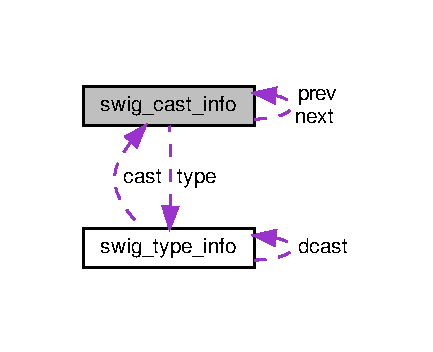
\includegraphics[width=208pt]{structswig__cast__info__coll__graph}
\end{center}
\end{figure}
\subsection*{Data Fields}
\begin{DoxyCompactItemize}
\item 
\hyperlink{structswig__type__info}{swig\+\_\+type\+\_\+info} $\ast$ \hyperlink{structswig__cast__info_a1c9023a301c8d6806209f4e10df6e9e0}{type}
\item 
\hyperlink{pdnsim__wrap_8cpp_a9a51597c7c2041da303a65468011f59b}{swig\+\_\+converter\+\_\+func} \hyperlink{structswig__cast__info_aa630fddfbb1bf9c97a03f9479ba32f76}{converter}
\item 
struct \hyperlink{structswig__cast__info}{swig\+\_\+cast\+\_\+info} $\ast$ \hyperlink{structswig__cast__info_ae79c6fa058a9d908bbdac14db0c9db5e}{next}
\item 
struct \hyperlink{structswig__cast__info}{swig\+\_\+cast\+\_\+info} $\ast$ \hyperlink{structswig__cast__info_afc685bcf38a5a06c6601775138c5999c}{prev}
\end{DoxyCompactItemize}


\subsection{Field Documentation}
\mbox{\Hypertarget{structswig__cast__info_aa630fddfbb1bf9c97a03f9479ba32f76}\label{structswig__cast__info_aa630fddfbb1bf9c97a03f9479ba32f76}} 
\index{swig\+\_\+cast\+\_\+info@{swig\+\_\+cast\+\_\+info}!converter@{converter}}
\index{converter@{converter}!swig\+\_\+cast\+\_\+info@{swig\+\_\+cast\+\_\+info}}
\subsubsection{\texorpdfstring{converter}{converter}}
{\footnotesize\ttfamily \hyperlink{pdnsim__wrap_8cpp_a9a51597c7c2041da303a65468011f59b}{swig\+\_\+converter\+\_\+func} swig\+\_\+cast\+\_\+info\+::converter}

\mbox{\Hypertarget{structswig__cast__info_ae79c6fa058a9d908bbdac14db0c9db5e}\label{structswig__cast__info_ae79c6fa058a9d908bbdac14db0c9db5e}} 
\index{swig\+\_\+cast\+\_\+info@{swig\+\_\+cast\+\_\+info}!next@{next}}
\index{next@{next}!swig\+\_\+cast\+\_\+info@{swig\+\_\+cast\+\_\+info}}
\subsubsection{\texorpdfstring{next}{next}}
{\footnotesize\ttfamily struct \hyperlink{structswig__cast__info}{swig\+\_\+cast\+\_\+info}$\ast$ swig\+\_\+cast\+\_\+info\+::next}

\mbox{\Hypertarget{structswig__cast__info_afc685bcf38a5a06c6601775138c5999c}\label{structswig__cast__info_afc685bcf38a5a06c6601775138c5999c}} 
\index{swig\+\_\+cast\+\_\+info@{swig\+\_\+cast\+\_\+info}!prev@{prev}}
\index{prev@{prev}!swig\+\_\+cast\+\_\+info@{swig\+\_\+cast\+\_\+info}}
\subsubsection{\texorpdfstring{prev}{prev}}
{\footnotesize\ttfamily struct \hyperlink{structswig__cast__info}{swig\+\_\+cast\+\_\+info}$\ast$ swig\+\_\+cast\+\_\+info\+::prev}

\mbox{\Hypertarget{structswig__cast__info_a1c9023a301c8d6806209f4e10df6e9e0}\label{structswig__cast__info_a1c9023a301c8d6806209f4e10df6e9e0}} 
\index{swig\+\_\+cast\+\_\+info@{swig\+\_\+cast\+\_\+info}!type@{type}}
\index{type@{type}!swig\+\_\+cast\+\_\+info@{swig\+\_\+cast\+\_\+info}}
\subsubsection{\texorpdfstring{type}{type}}
{\footnotesize\ttfamily \hyperlink{structswig__type__info}{swig\+\_\+type\+\_\+info}$\ast$ swig\+\_\+cast\+\_\+info\+::type}



The documentation for this struct was generated from the following file\+:\begin{DoxyCompactItemize}
\item 
src/\hyperlink{pdnsim__wrap_8cpp}{pdnsim\+\_\+wrap.\+cpp}\end{DoxyCompactItemize}

\hypertarget{structswig__class}{}\section{swig\+\_\+class Struct Reference}
\label{structswig__class}\index{swig\+\_\+class@{swig\+\_\+class}}


Collaboration diagram for swig\+\_\+class\+:\nopagebreak
\begin{figure}[H]
\begin{center}
\leavevmode
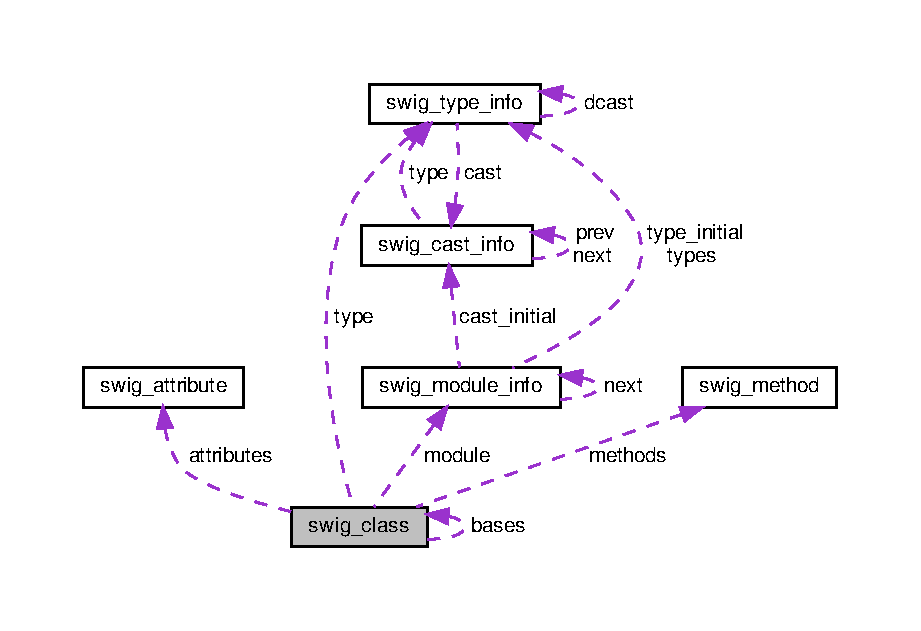
\includegraphics[width=350pt]{structswig__class__coll__graph}
\end{center}
\end{figure}
\subsection*{Data Fields}
\begin{DoxyCompactItemize}
\item 
const char $\ast$ \hyperlink{structswig__class_a4f5616c467aa85a1ee98302174a9a274}{name}
\item 
\hyperlink{structswig__type__info}{swig\+\_\+type\+\_\+info} $\ast$$\ast$ \hyperlink{structswig__class_ad003f6193cbabe3b78293db9914bc3e6}{type}
\item 
\hyperlink{pdnsim__wrap_8cpp_a26e4d1918011eb5b4aa36f67e1d5a318}{swig\+\_\+wrapper} \hyperlink{structswig__class_a943365b5944f3beb08271d297475da3f}{constructor}
\item 
void($\ast$ \hyperlink{structswig__class_a7b990b9ef92362180df695db37f1fb2a}{destructor} )(void $\ast$)
\item 
\hyperlink{structswig__method}{swig\+\_\+method} $\ast$ \hyperlink{structswig__class_ad4a9ded260af27126bd0e2ec70b651c2}{methods}
\item 
\hyperlink{structswig__attribute}{swig\+\_\+attribute} $\ast$ \hyperlink{structswig__class_a2a73cdf08c947e5ecce4138c0f9b69f1}{attributes}
\item 
struct \hyperlink{structswig__class}{swig\+\_\+class} $\ast$$\ast$ \hyperlink{structswig__class_a8208d113d09eb3f2774ef7ff8b1b1308}{bases}
\item 
const char $\ast$$\ast$ \hyperlink{structswig__class_a3e98c300724371a0fcffed2293a54f9c}{base\+\_\+names}
\item 
\hyperlink{structswig__module__info}{swig\+\_\+module\+\_\+info} $\ast$ \hyperlink{structswig__class_ac8105783928c259f2b79e1329afbdcdb}{module}
\item 
Tcl\+\_\+\+Hash\+Table \hyperlink{structswig__class_a507bd16a0168767b18cd40a9be9d7516}{hashtable}
\end{DoxyCompactItemize}


\subsection{Field Documentation}
\mbox{\Hypertarget{structswig__class_a2a73cdf08c947e5ecce4138c0f9b69f1}\label{structswig__class_a2a73cdf08c947e5ecce4138c0f9b69f1}} 
\index{swig\+\_\+class@{swig\+\_\+class}!attributes@{attributes}}
\index{attributes@{attributes}!swig\+\_\+class@{swig\+\_\+class}}
\subsubsection{\texorpdfstring{attributes}{attributes}}
{\footnotesize\ttfamily \hyperlink{structswig__attribute}{swig\+\_\+attribute}$\ast$ swig\+\_\+class\+::attributes}

\mbox{\Hypertarget{structswig__class_a3e98c300724371a0fcffed2293a54f9c}\label{structswig__class_a3e98c300724371a0fcffed2293a54f9c}} 
\index{swig\+\_\+class@{swig\+\_\+class}!base\+\_\+names@{base\+\_\+names}}
\index{base\+\_\+names@{base\+\_\+names}!swig\+\_\+class@{swig\+\_\+class}}
\subsubsection{\texorpdfstring{base\+\_\+names}{base\_names}}
{\footnotesize\ttfamily const char$\ast$$\ast$ swig\+\_\+class\+::base\+\_\+names}

\mbox{\Hypertarget{structswig__class_a8208d113d09eb3f2774ef7ff8b1b1308}\label{structswig__class_a8208d113d09eb3f2774ef7ff8b1b1308}} 
\index{swig\+\_\+class@{swig\+\_\+class}!bases@{bases}}
\index{bases@{bases}!swig\+\_\+class@{swig\+\_\+class}}
\subsubsection{\texorpdfstring{bases}{bases}}
{\footnotesize\ttfamily struct \hyperlink{structswig__class}{swig\+\_\+class}$\ast$$\ast$ swig\+\_\+class\+::bases}

\mbox{\Hypertarget{structswig__class_a943365b5944f3beb08271d297475da3f}\label{structswig__class_a943365b5944f3beb08271d297475da3f}} 
\index{swig\+\_\+class@{swig\+\_\+class}!constructor@{constructor}}
\index{constructor@{constructor}!swig\+\_\+class@{swig\+\_\+class}}
\subsubsection{\texorpdfstring{constructor}{constructor}}
{\footnotesize\ttfamily \hyperlink{pdnsim__wrap_8cpp_a26e4d1918011eb5b4aa36f67e1d5a318}{swig\+\_\+wrapper} swig\+\_\+class\+::constructor}

\mbox{\Hypertarget{structswig__class_a7b990b9ef92362180df695db37f1fb2a}\label{structswig__class_a7b990b9ef92362180df695db37f1fb2a}} 
\index{swig\+\_\+class@{swig\+\_\+class}!destructor@{destructor}}
\index{destructor@{destructor}!swig\+\_\+class@{swig\+\_\+class}}
\subsubsection{\texorpdfstring{destructor}{destructor}}
{\footnotesize\ttfamily void($\ast$ swig\+\_\+class\+::destructor) (void $\ast$)}

\mbox{\Hypertarget{structswig__class_a507bd16a0168767b18cd40a9be9d7516}\label{structswig__class_a507bd16a0168767b18cd40a9be9d7516}} 
\index{swig\+\_\+class@{swig\+\_\+class}!hashtable@{hashtable}}
\index{hashtable@{hashtable}!swig\+\_\+class@{swig\+\_\+class}}
\subsubsection{\texorpdfstring{hashtable}{hashtable}}
{\footnotesize\ttfamily Tcl\+\_\+\+Hash\+Table swig\+\_\+class\+::hashtable}

\mbox{\Hypertarget{structswig__class_ad4a9ded260af27126bd0e2ec70b651c2}\label{structswig__class_ad4a9ded260af27126bd0e2ec70b651c2}} 
\index{swig\+\_\+class@{swig\+\_\+class}!methods@{methods}}
\index{methods@{methods}!swig\+\_\+class@{swig\+\_\+class}}
\subsubsection{\texorpdfstring{methods}{methods}}
{\footnotesize\ttfamily \hyperlink{structswig__method}{swig\+\_\+method}$\ast$ swig\+\_\+class\+::methods}

\mbox{\Hypertarget{structswig__class_ac8105783928c259f2b79e1329afbdcdb}\label{structswig__class_ac8105783928c259f2b79e1329afbdcdb}} 
\index{swig\+\_\+class@{swig\+\_\+class}!module@{module}}
\index{module@{module}!swig\+\_\+class@{swig\+\_\+class}}
\subsubsection{\texorpdfstring{module}{module}}
{\footnotesize\ttfamily \hyperlink{structswig__module__info}{swig\+\_\+module\+\_\+info}$\ast$ swig\+\_\+class\+::module}

\mbox{\Hypertarget{structswig__class_a4f5616c467aa85a1ee98302174a9a274}\label{structswig__class_a4f5616c467aa85a1ee98302174a9a274}} 
\index{swig\+\_\+class@{swig\+\_\+class}!name@{name}}
\index{name@{name}!swig\+\_\+class@{swig\+\_\+class}}
\subsubsection{\texorpdfstring{name}{name}}
{\footnotesize\ttfamily const char$\ast$ swig\+\_\+class\+::name}

\mbox{\Hypertarget{structswig__class_ad003f6193cbabe3b78293db9914bc3e6}\label{structswig__class_ad003f6193cbabe3b78293db9914bc3e6}} 
\index{swig\+\_\+class@{swig\+\_\+class}!type@{type}}
\index{type@{type}!swig\+\_\+class@{swig\+\_\+class}}
\subsubsection{\texorpdfstring{type}{type}}
{\footnotesize\ttfamily \hyperlink{structswig__type__info}{swig\+\_\+type\+\_\+info}$\ast$$\ast$ swig\+\_\+class\+::type}



The documentation for this struct was generated from the following file\+:\begin{DoxyCompactItemize}
\item 
src/\hyperlink{pdnsim__wrap_8cpp}{pdnsim\+\_\+wrap.\+cpp}\end{DoxyCompactItemize}

\hypertarget{structswig__command__info}{}\section{swig\+\_\+command\+\_\+info Struct Reference}
\label{structswig__command__info}\index{swig\+\_\+command\+\_\+info@{swig\+\_\+command\+\_\+info}}
\subsection*{Data Fields}
\begin{DoxyCompactItemize}
\item 
const char $\ast$ \hyperlink{structswig__command__info_a5c3fec9159e5dc6429b27889dd9a903d}{name}
\item 
int($\ast$ \hyperlink{structswig__command__info_acd779e4b3dc31b81f4e40b6f06128bea}{wrapper} )(Client\+Data, Tcl\+\_\+\+Interp $\ast$, int, Tcl\+\_\+\+Obj $\ast$C\+O\+N\+ST \mbox{[}$\,$\mbox{]})
\item 
Client\+Data \hyperlink{structswig__command__info_a7418da5fdc25428d9cebfb6da0c6f6f2}{clientdata}
\end{DoxyCompactItemize}


\subsection{Field Documentation}
\mbox{\Hypertarget{structswig__command__info_a7418da5fdc25428d9cebfb6da0c6f6f2}\label{structswig__command__info_a7418da5fdc25428d9cebfb6da0c6f6f2}} 
\index{swig\+\_\+command\+\_\+info@{swig\+\_\+command\+\_\+info}!clientdata@{clientdata}}
\index{clientdata@{clientdata}!swig\+\_\+command\+\_\+info@{swig\+\_\+command\+\_\+info}}
\subsubsection{\texorpdfstring{clientdata}{clientdata}}
{\footnotesize\ttfamily Client\+Data swig\+\_\+command\+\_\+info\+::clientdata}

\mbox{\Hypertarget{structswig__command__info_a5c3fec9159e5dc6429b27889dd9a903d}\label{structswig__command__info_a5c3fec9159e5dc6429b27889dd9a903d}} 
\index{swig\+\_\+command\+\_\+info@{swig\+\_\+command\+\_\+info}!name@{name}}
\index{name@{name}!swig\+\_\+command\+\_\+info@{swig\+\_\+command\+\_\+info}}
\subsubsection{\texorpdfstring{name}{name}}
{\footnotesize\ttfamily const char$\ast$ swig\+\_\+command\+\_\+info\+::name}

\mbox{\Hypertarget{structswig__command__info_acd779e4b3dc31b81f4e40b6f06128bea}\label{structswig__command__info_acd779e4b3dc31b81f4e40b6f06128bea}} 
\index{swig\+\_\+command\+\_\+info@{swig\+\_\+command\+\_\+info}!wrapper@{wrapper}}
\index{wrapper@{wrapper}!swig\+\_\+command\+\_\+info@{swig\+\_\+command\+\_\+info}}
\subsubsection{\texorpdfstring{wrapper}{wrapper}}
{\footnotesize\ttfamily int($\ast$ swig\+\_\+command\+\_\+info\+::wrapper) (Client\+Data, Tcl\+\_\+\+Interp $\ast$, int, Tcl\+\_\+\+Obj $\ast$C\+O\+N\+ST \mbox{[}$\,$\mbox{]})}



The documentation for this struct was generated from the following file\+:\begin{DoxyCompactItemize}
\item 
src/\hyperlink{pdnsim__wrap_8cpp}{pdnsim\+\_\+wrap.\+cpp}\end{DoxyCompactItemize}

\hypertarget{structswig__const__info}{}\section{swig\+\_\+const\+\_\+info Struct Reference}
\label{structswig__const__info}\index{swig\+\_\+const\+\_\+info@{swig\+\_\+const\+\_\+info}}


Collaboration diagram for swig\+\_\+const\+\_\+info\+:\nopagebreak
\begin{figure}[H]
\begin{center}
\leavevmode
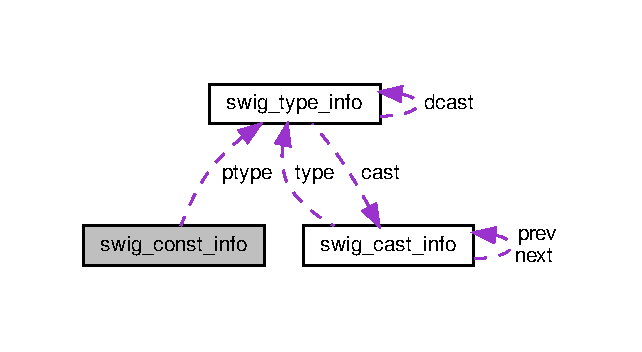
\includegraphics[width=308pt]{structswig__const__info__coll__graph}
\end{center}
\end{figure}
\subsection*{Data Fields}
\begin{DoxyCompactItemize}
\item 
int \hyperlink{structswig__const__info_ae8bbc99e1cda11f24e306365cbf33893}{type}
\item 
char $\ast$ \hyperlink{structswig__const__info_aad383d74116313cf9a8532e163368050}{name}
\item 
long \hyperlink{structswig__const__info_af142e4c21ad4fe61f6c2624bff034583}{lvalue}
\item 
double \hyperlink{structswig__const__info_a74e477f1dbf515bcb7e2ef07a1d34c35}{dvalue}
\item 
void $\ast$ \hyperlink{structswig__const__info_abbc43512c364bff11fac5961c1155090}{pvalue}
\item 
\hyperlink{structswig__type__info}{swig\+\_\+type\+\_\+info} $\ast$$\ast$ \hyperlink{structswig__const__info_aedd46d173c5b5ed4ee60ad5660233557}{ptype}
\end{DoxyCompactItemize}


\subsection{Field Documentation}
\mbox{\Hypertarget{structswig__const__info_a74e477f1dbf515bcb7e2ef07a1d34c35}\label{structswig__const__info_a74e477f1dbf515bcb7e2ef07a1d34c35}} 
\index{swig\+\_\+const\+\_\+info@{swig\+\_\+const\+\_\+info}!dvalue@{dvalue}}
\index{dvalue@{dvalue}!swig\+\_\+const\+\_\+info@{swig\+\_\+const\+\_\+info}}
\subsubsection{\texorpdfstring{dvalue}{dvalue}}
{\footnotesize\ttfamily double swig\+\_\+const\+\_\+info\+::dvalue}

\mbox{\Hypertarget{structswig__const__info_af142e4c21ad4fe61f6c2624bff034583}\label{structswig__const__info_af142e4c21ad4fe61f6c2624bff034583}} 
\index{swig\+\_\+const\+\_\+info@{swig\+\_\+const\+\_\+info}!lvalue@{lvalue}}
\index{lvalue@{lvalue}!swig\+\_\+const\+\_\+info@{swig\+\_\+const\+\_\+info}}
\subsubsection{\texorpdfstring{lvalue}{lvalue}}
{\footnotesize\ttfamily long swig\+\_\+const\+\_\+info\+::lvalue}

\mbox{\Hypertarget{structswig__const__info_aad383d74116313cf9a8532e163368050}\label{structswig__const__info_aad383d74116313cf9a8532e163368050}} 
\index{swig\+\_\+const\+\_\+info@{swig\+\_\+const\+\_\+info}!name@{name}}
\index{name@{name}!swig\+\_\+const\+\_\+info@{swig\+\_\+const\+\_\+info}}
\subsubsection{\texorpdfstring{name}{name}}
{\footnotesize\ttfamily char$\ast$ swig\+\_\+const\+\_\+info\+::name}

\mbox{\Hypertarget{structswig__const__info_aedd46d173c5b5ed4ee60ad5660233557}\label{structswig__const__info_aedd46d173c5b5ed4ee60ad5660233557}} 
\index{swig\+\_\+const\+\_\+info@{swig\+\_\+const\+\_\+info}!ptype@{ptype}}
\index{ptype@{ptype}!swig\+\_\+const\+\_\+info@{swig\+\_\+const\+\_\+info}}
\subsubsection{\texorpdfstring{ptype}{ptype}}
{\footnotesize\ttfamily \hyperlink{structswig__type__info}{swig\+\_\+type\+\_\+info}$\ast$$\ast$ swig\+\_\+const\+\_\+info\+::ptype}

\mbox{\Hypertarget{structswig__const__info_abbc43512c364bff11fac5961c1155090}\label{structswig__const__info_abbc43512c364bff11fac5961c1155090}} 
\index{swig\+\_\+const\+\_\+info@{swig\+\_\+const\+\_\+info}!pvalue@{pvalue}}
\index{pvalue@{pvalue}!swig\+\_\+const\+\_\+info@{swig\+\_\+const\+\_\+info}}
\subsubsection{\texorpdfstring{pvalue}{pvalue}}
{\footnotesize\ttfamily void$\ast$ swig\+\_\+const\+\_\+info\+::pvalue}

\mbox{\Hypertarget{structswig__const__info_ae8bbc99e1cda11f24e306365cbf33893}\label{structswig__const__info_ae8bbc99e1cda11f24e306365cbf33893}} 
\index{swig\+\_\+const\+\_\+info@{swig\+\_\+const\+\_\+info}!type@{type}}
\index{type@{type}!swig\+\_\+const\+\_\+info@{swig\+\_\+const\+\_\+info}}
\subsubsection{\texorpdfstring{type}{type}}
{\footnotesize\ttfamily int swig\+\_\+const\+\_\+info\+::type}



The documentation for this struct was generated from the following file\+:\begin{DoxyCompactItemize}
\item 
src/\hyperlink{pdnsim__wrap_8cpp}{pdnsim\+\_\+wrap.\+cpp}\end{DoxyCompactItemize}

\hypertarget{structswig__instance}{}\section{swig\+\_\+instance Struct Reference}
\label{structswig__instance}\index{swig\+\_\+instance@{swig\+\_\+instance}}


Collaboration diagram for swig\+\_\+instance\+:\nopagebreak
\begin{figure}[H]
\begin{center}
\leavevmode
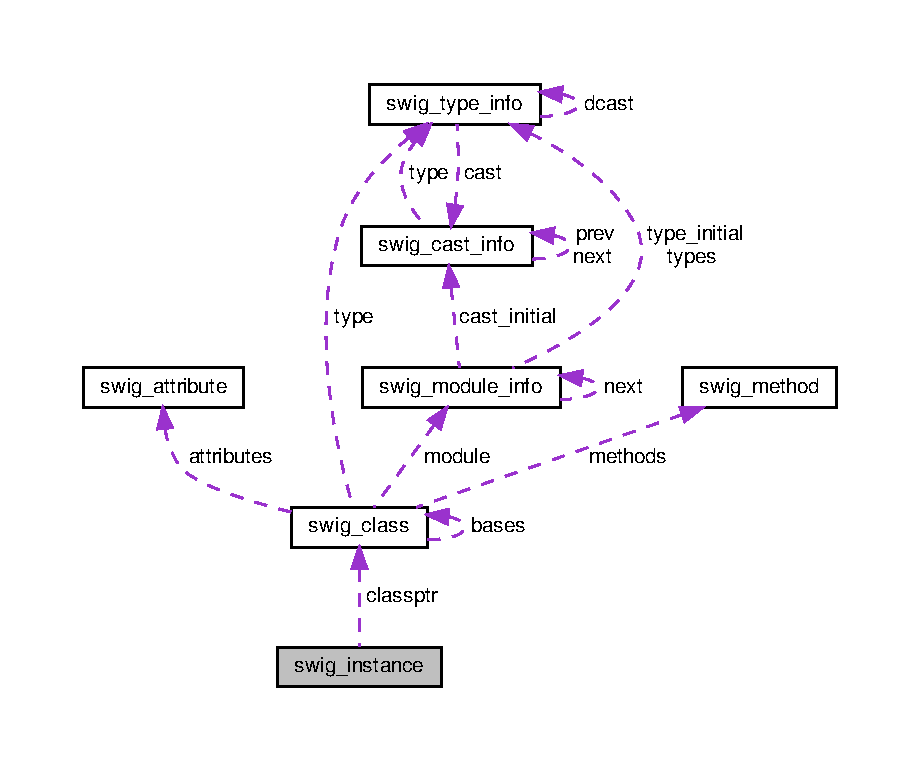
\includegraphics[width=350pt]{structswig__instance__coll__graph}
\end{center}
\end{figure}
\subsection*{Data Fields}
\begin{DoxyCompactItemize}
\item 
Tcl\+\_\+\+Obj $\ast$ \hyperlink{structswig__instance_ad53df21eb34277cc516a5011451a5762}{thisptr}
\item 
void $\ast$ \hyperlink{structswig__instance_a896fc81e257c64aae217eb80543f1632}{thisvalue}
\item 
\hyperlink{structswig__class}{swig\+\_\+class} $\ast$ \hyperlink{structswig__instance_a3ac823647cceb84f1fc42aa0b2b95f53}{classptr}
\item 
int \hyperlink{structswig__instance_a3bdcd16ae587f72dd6e29e52745e279a}{destroy}
\item 
Tcl\+\_\+\+Command \hyperlink{structswig__instance_a922b8e6fb63293c195d7de91086d0cad}{cmdtok}
\end{DoxyCompactItemize}


\subsection{Field Documentation}
\mbox{\Hypertarget{structswig__instance_a3ac823647cceb84f1fc42aa0b2b95f53}\label{structswig__instance_a3ac823647cceb84f1fc42aa0b2b95f53}} 
\index{swig\+\_\+instance@{swig\+\_\+instance}!classptr@{classptr}}
\index{classptr@{classptr}!swig\+\_\+instance@{swig\+\_\+instance}}
\subsubsection{\texorpdfstring{classptr}{classptr}}
{\footnotesize\ttfamily \hyperlink{structswig__class}{swig\+\_\+class}$\ast$ swig\+\_\+instance\+::classptr}

\mbox{\Hypertarget{structswig__instance_a922b8e6fb63293c195d7de91086d0cad}\label{structswig__instance_a922b8e6fb63293c195d7de91086d0cad}} 
\index{swig\+\_\+instance@{swig\+\_\+instance}!cmdtok@{cmdtok}}
\index{cmdtok@{cmdtok}!swig\+\_\+instance@{swig\+\_\+instance}}
\subsubsection{\texorpdfstring{cmdtok}{cmdtok}}
{\footnotesize\ttfamily Tcl\+\_\+\+Command swig\+\_\+instance\+::cmdtok}

\mbox{\Hypertarget{structswig__instance_a3bdcd16ae587f72dd6e29e52745e279a}\label{structswig__instance_a3bdcd16ae587f72dd6e29e52745e279a}} 
\index{swig\+\_\+instance@{swig\+\_\+instance}!destroy@{destroy}}
\index{destroy@{destroy}!swig\+\_\+instance@{swig\+\_\+instance}}
\subsubsection{\texorpdfstring{destroy}{destroy}}
{\footnotesize\ttfamily int swig\+\_\+instance\+::destroy}

\mbox{\Hypertarget{structswig__instance_ad53df21eb34277cc516a5011451a5762}\label{structswig__instance_ad53df21eb34277cc516a5011451a5762}} 
\index{swig\+\_\+instance@{swig\+\_\+instance}!thisptr@{thisptr}}
\index{thisptr@{thisptr}!swig\+\_\+instance@{swig\+\_\+instance}}
\subsubsection{\texorpdfstring{thisptr}{thisptr}}
{\footnotesize\ttfamily Tcl\+\_\+\+Obj$\ast$ swig\+\_\+instance\+::thisptr}

\mbox{\Hypertarget{structswig__instance_a896fc81e257c64aae217eb80543f1632}\label{structswig__instance_a896fc81e257c64aae217eb80543f1632}} 
\index{swig\+\_\+instance@{swig\+\_\+instance}!thisvalue@{thisvalue}}
\index{thisvalue@{thisvalue}!swig\+\_\+instance@{swig\+\_\+instance}}
\subsubsection{\texorpdfstring{thisvalue}{thisvalue}}
{\footnotesize\ttfamily void$\ast$ swig\+\_\+instance\+::thisvalue}



The documentation for this struct was generated from the following file\+:\begin{DoxyCompactItemize}
\item 
src/\hyperlink{pdnsim__wrap_8cpp}{pdnsim\+\_\+wrap.\+cpp}\end{DoxyCompactItemize}

\hypertarget{structswig__method}{}\section{swig\+\_\+method Struct Reference}
\label{structswig__method}\index{swig\+\_\+method@{swig\+\_\+method}}
\subsection*{Data Fields}
\begin{DoxyCompactItemize}
\item 
const char $\ast$ \hyperlink{structswig__method_ac49e680ac1d2b0255de147c5f3ec44d2}{name}
\item 
\hyperlink{pdnsim__wrap_8cpp_a26e4d1918011eb5b4aa36f67e1d5a318}{swig\+\_\+wrapper} \hyperlink{structswig__method_ad2006ee1cedbefd358f704920d9ecad0}{method}
\end{DoxyCompactItemize}


\subsection{Field Documentation}
\mbox{\Hypertarget{structswig__method_ad2006ee1cedbefd358f704920d9ecad0}\label{structswig__method_ad2006ee1cedbefd358f704920d9ecad0}} 
\index{swig\+\_\+method@{swig\+\_\+method}!method@{method}}
\index{method@{method}!swig\+\_\+method@{swig\+\_\+method}}
\subsubsection{\texorpdfstring{method}{method}}
{\footnotesize\ttfamily \hyperlink{pdnsim__wrap_8cpp_a26e4d1918011eb5b4aa36f67e1d5a318}{swig\+\_\+wrapper} swig\+\_\+method\+::method}

\mbox{\Hypertarget{structswig__method_ac49e680ac1d2b0255de147c5f3ec44d2}\label{structswig__method_ac49e680ac1d2b0255de147c5f3ec44d2}} 
\index{swig\+\_\+method@{swig\+\_\+method}!name@{name}}
\index{name@{name}!swig\+\_\+method@{swig\+\_\+method}}
\subsubsection{\texorpdfstring{name}{name}}
{\footnotesize\ttfamily const char$\ast$ swig\+\_\+method\+::name}



The documentation for this struct was generated from the following file\+:\begin{DoxyCompactItemize}
\item 
src/\hyperlink{pdnsim__wrap_8cpp}{pdnsim\+\_\+wrap.\+cpp}\end{DoxyCompactItemize}

\hypertarget{structswig__module__info}{}\section{swig\+\_\+module\+\_\+info Struct Reference}
\label{structswig__module__info}\index{swig\+\_\+module\+\_\+info@{swig\+\_\+module\+\_\+info}}


Collaboration diagram for swig\+\_\+module\+\_\+info\+:\nopagebreak
\begin{figure}[H]
\begin{center}
\leavevmode
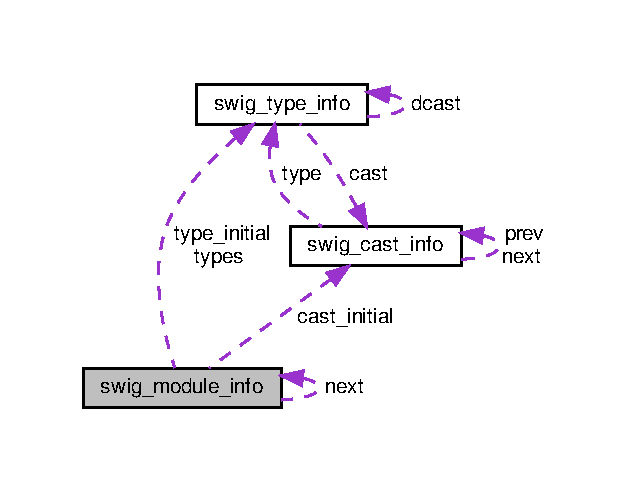
\includegraphics[width=302pt]{structswig__module__info__coll__graph}
\end{center}
\end{figure}
\subsection*{Data Fields}
\begin{DoxyCompactItemize}
\item 
\hyperlink{structswig__type__info}{swig\+\_\+type\+\_\+info} $\ast$$\ast$ \hyperlink{structswig__module__info_ad658c7738e9a035ef8eea865322fbf13}{types}
\item 
size\+\_\+t \hyperlink{structswig__module__info_aaf8907cf8509ee0464af8c9dfd909042}{size}
\item 
struct \hyperlink{structswig__module__info}{swig\+\_\+module\+\_\+info} $\ast$ \hyperlink{structswig__module__info_ac177d150b85ab77122089acf1f06d9c6}{next}
\item 
\hyperlink{structswig__type__info}{swig\+\_\+type\+\_\+info} $\ast$$\ast$ \hyperlink{structswig__module__info_a76c7d5b0fc10371748616d0b6c815a17}{type\+\_\+initial}
\item 
\hyperlink{structswig__cast__info}{swig\+\_\+cast\+\_\+info} $\ast$$\ast$ \hyperlink{structswig__module__info_a15f6b50a41f144afb1148fc412dc01f7}{cast\+\_\+initial}
\item 
void $\ast$ \hyperlink{structswig__module__info_a9fb6e461fcaf14c209049adfae4e9754}{clientdata}
\end{DoxyCompactItemize}


\subsection{Field Documentation}
\mbox{\Hypertarget{structswig__module__info_a15f6b50a41f144afb1148fc412dc01f7}\label{structswig__module__info_a15f6b50a41f144afb1148fc412dc01f7}} 
\index{swig\+\_\+module\+\_\+info@{swig\+\_\+module\+\_\+info}!cast\+\_\+initial@{cast\+\_\+initial}}
\index{cast\+\_\+initial@{cast\+\_\+initial}!swig\+\_\+module\+\_\+info@{swig\+\_\+module\+\_\+info}}
\subsubsection{\texorpdfstring{cast\+\_\+initial}{cast\_initial}}
{\footnotesize\ttfamily \hyperlink{structswig__cast__info}{swig\+\_\+cast\+\_\+info}$\ast$$\ast$ swig\+\_\+module\+\_\+info\+::cast\+\_\+initial}

\mbox{\Hypertarget{structswig__module__info_a9fb6e461fcaf14c209049adfae4e9754}\label{structswig__module__info_a9fb6e461fcaf14c209049adfae4e9754}} 
\index{swig\+\_\+module\+\_\+info@{swig\+\_\+module\+\_\+info}!clientdata@{clientdata}}
\index{clientdata@{clientdata}!swig\+\_\+module\+\_\+info@{swig\+\_\+module\+\_\+info}}
\subsubsection{\texorpdfstring{clientdata}{clientdata}}
{\footnotesize\ttfamily void$\ast$ swig\+\_\+module\+\_\+info\+::clientdata}

\mbox{\Hypertarget{structswig__module__info_ac177d150b85ab77122089acf1f06d9c6}\label{structswig__module__info_ac177d150b85ab77122089acf1f06d9c6}} 
\index{swig\+\_\+module\+\_\+info@{swig\+\_\+module\+\_\+info}!next@{next}}
\index{next@{next}!swig\+\_\+module\+\_\+info@{swig\+\_\+module\+\_\+info}}
\subsubsection{\texorpdfstring{next}{next}}
{\footnotesize\ttfamily struct \hyperlink{structswig__module__info}{swig\+\_\+module\+\_\+info}$\ast$ swig\+\_\+module\+\_\+info\+::next}

\mbox{\Hypertarget{structswig__module__info_aaf8907cf8509ee0464af8c9dfd909042}\label{structswig__module__info_aaf8907cf8509ee0464af8c9dfd909042}} 
\index{swig\+\_\+module\+\_\+info@{swig\+\_\+module\+\_\+info}!size@{size}}
\index{size@{size}!swig\+\_\+module\+\_\+info@{swig\+\_\+module\+\_\+info}}
\subsubsection{\texorpdfstring{size}{size}}
{\footnotesize\ttfamily size\+\_\+t swig\+\_\+module\+\_\+info\+::size}

\mbox{\Hypertarget{structswig__module__info_a76c7d5b0fc10371748616d0b6c815a17}\label{structswig__module__info_a76c7d5b0fc10371748616d0b6c815a17}} 
\index{swig\+\_\+module\+\_\+info@{swig\+\_\+module\+\_\+info}!type\+\_\+initial@{type\+\_\+initial}}
\index{type\+\_\+initial@{type\+\_\+initial}!swig\+\_\+module\+\_\+info@{swig\+\_\+module\+\_\+info}}
\subsubsection{\texorpdfstring{type\+\_\+initial}{type\_initial}}
{\footnotesize\ttfamily \hyperlink{structswig__type__info}{swig\+\_\+type\+\_\+info}$\ast$$\ast$ swig\+\_\+module\+\_\+info\+::type\+\_\+initial}

\mbox{\Hypertarget{structswig__module__info_ad658c7738e9a035ef8eea865322fbf13}\label{structswig__module__info_ad658c7738e9a035ef8eea865322fbf13}} 
\index{swig\+\_\+module\+\_\+info@{swig\+\_\+module\+\_\+info}!types@{types}}
\index{types@{types}!swig\+\_\+module\+\_\+info@{swig\+\_\+module\+\_\+info}}
\subsubsection{\texorpdfstring{types}{types}}
{\footnotesize\ttfamily \hyperlink{structswig__type__info}{swig\+\_\+type\+\_\+info}$\ast$$\ast$ swig\+\_\+module\+\_\+info\+::types}



The documentation for this struct was generated from the following file\+:\begin{DoxyCompactItemize}
\item 
src/\hyperlink{pdnsim__wrap_8cpp}{pdnsim\+\_\+wrap.\+cpp}\end{DoxyCompactItemize}

\hypertarget{structswig__type__info}{}\section{swig\+\_\+type\+\_\+info Struct Reference}
\label{structswig__type__info}\index{swig\+\_\+type\+\_\+info@{swig\+\_\+type\+\_\+info}}


Collaboration diagram for swig\+\_\+type\+\_\+info\+:\nopagebreak
\begin{figure}[H]
\begin{center}
\leavevmode
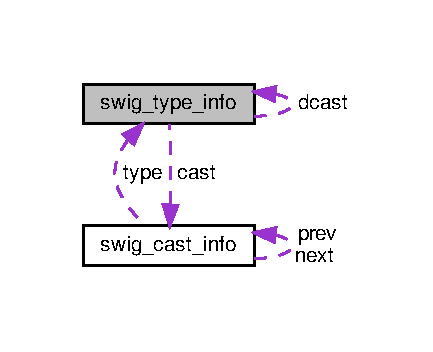
\includegraphics[width=208pt]{structswig__type__info__coll__graph}
\end{center}
\end{figure}
\subsection*{Data Fields}
\begin{DoxyCompactItemize}
\item 
const char $\ast$ \hyperlink{structswig__type__info_a90a9c6a25aa3e923978005ecbe23ad60}{name}
\item 
const char $\ast$ \hyperlink{structswig__type__info_abbe7cc58a083feb4329b748643324064}{str}
\item 
\hyperlink{pdnsim__wrap_8cpp_aee981c41d733723d60337a77630106af}{swig\+\_\+dycast\+\_\+func} \hyperlink{structswig__type__info_a07df4bedf85be77b23756b531b60e0dd}{dcast}
\item 
struct \hyperlink{structswig__cast__info}{swig\+\_\+cast\+\_\+info} $\ast$ \hyperlink{structswig__type__info_a3ee3f7ef20e965b6c798d79723a96f9b}{cast}
\item 
void $\ast$ \hyperlink{structswig__type__info_a19bdd65dceb89cd54befd3ded06558b7}{clientdata}
\item 
int \hyperlink{structswig__type__info_a93c25d5903cbfcb82208eea7227c32bd}{owndata}
\end{DoxyCompactItemize}


\subsection{Field Documentation}
\mbox{\Hypertarget{structswig__type__info_a3ee3f7ef20e965b6c798d79723a96f9b}\label{structswig__type__info_a3ee3f7ef20e965b6c798d79723a96f9b}} 
\index{swig\+\_\+type\+\_\+info@{swig\+\_\+type\+\_\+info}!cast@{cast}}
\index{cast@{cast}!swig\+\_\+type\+\_\+info@{swig\+\_\+type\+\_\+info}}
\subsubsection{\texorpdfstring{cast}{cast}}
{\footnotesize\ttfamily struct \hyperlink{structswig__cast__info}{swig\+\_\+cast\+\_\+info}$\ast$ swig\+\_\+type\+\_\+info\+::cast}

\mbox{\Hypertarget{structswig__type__info_a19bdd65dceb89cd54befd3ded06558b7}\label{structswig__type__info_a19bdd65dceb89cd54befd3ded06558b7}} 
\index{swig\+\_\+type\+\_\+info@{swig\+\_\+type\+\_\+info}!clientdata@{clientdata}}
\index{clientdata@{clientdata}!swig\+\_\+type\+\_\+info@{swig\+\_\+type\+\_\+info}}
\subsubsection{\texorpdfstring{clientdata}{clientdata}}
{\footnotesize\ttfamily void$\ast$ swig\+\_\+type\+\_\+info\+::clientdata}

\mbox{\Hypertarget{structswig__type__info_a07df4bedf85be77b23756b531b60e0dd}\label{structswig__type__info_a07df4bedf85be77b23756b531b60e0dd}} 
\index{swig\+\_\+type\+\_\+info@{swig\+\_\+type\+\_\+info}!dcast@{dcast}}
\index{dcast@{dcast}!swig\+\_\+type\+\_\+info@{swig\+\_\+type\+\_\+info}}
\subsubsection{\texorpdfstring{dcast}{dcast}}
{\footnotesize\ttfamily \hyperlink{pdnsim__wrap_8cpp_aee981c41d733723d60337a77630106af}{swig\+\_\+dycast\+\_\+func} swig\+\_\+type\+\_\+info\+::dcast}

\mbox{\Hypertarget{structswig__type__info_a90a9c6a25aa3e923978005ecbe23ad60}\label{structswig__type__info_a90a9c6a25aa3e923978005ecbe23ad60}} 
\index{swig\+\_\+type\+\_\+info@{swig\+\_\+type\+\_\+info}!name@{name}}
\index{name@{name}!swig\+\_\+type\+\_\+info@{swig\+\_\+type\+\_\+info}}
\subsubsection{\texorpdfstring{name}{name}}
{\footnotesize\ttfamily const char$\ast$ swig\+\_\+type\+\_\+info\+::name}

\mbox{\Hypertarget{structswig__type__info_a93c25d5903cbfcb82208eea7227c32bd}\label{structswig__type__info_a93c25d5903cbfcb82208eea7227c32bd}} 
\index{swig\+\_\+type\+\_\+info@{swig\+\_\+type\+\_\+info}!owndata@{owndata}}
\index{owndata@{owndata}!swig\+\_\+type\+\_\+info@{swig\+\_\+type\+\_\+info}}
\subsubsection{\texorpdfstring{owndata}{owndata}}
{\footnotesize\ttfamily int swig\+\_\+type\+\_\+info\+::owndata}

\mbox{\Hypertarget{structswig__type__info_abbe7cc58a083feb4329b748643324064}\label{structswig__type__info_abbe7cc58a083feb4329b748643324064}} 
\index{swig\+\_\+type\+\_\+info@{swig\+\_\+type\+\_\+info}!str@{str}}
\index{str@{str}!swig\+\_\+type\+\_\+info@{swig\+\_\+type\+\_\+info}}
\subsubsection{\texorpdfstring{str}{str}}
{\footnotesize\ttfamily const char$\ast$ swig\+\_\+type\+\_\+info\+::str}



The documentation for this struct was generated from the following file\+:\begin{DoxyCompactItemize}
\item 
src/\hyperlink{pdnsim__wrap_8cpp}{pdnsim\+\_\+wrap.\+cpp}\end{DoxyCompactItemize}

\hypertarget{structswig__var__info}{}\section{swig\+\_\+var\+\_\+info Struct Reference}
\label{structswig__var__info}\index{swig\+\_\+var\+\_\+info@{swig\+\_\+var\+\_\+info}}
\subsection*{Data Fields}
\begin{DoxyCompactItemize}
\item 
const char $\ast$ \hyperlink{structswig__var__info_a818f171973e6e1135a46b8b918c0b9eb}{name}
\item 
void $\ast$ \hyperlink{structswig__var__info_a8aefe7e94367ddbab2d090d913232b4f}{addr}
\item 
char $\ast$($\ast$ \hyperlink{structswig__var__info_a2077b465ca9dbaa90d7ca67eae508bf2}{get} )(Client\+Data, Tcl\+\_\+\+Interp $\ast$, char $\ast$, char $\ast$, int)
\item 
char $\ast$($\ast$ \hyperlink{structswig__var__info_a1c988d1806abe81050d325cc12524608}{set} )(Client\+Data, Tcl\+\_\+\+Interp $\ast$, char $\ast$, char $\ast$, int)
\end{DoxyCompactItemize}


\subsection{Field Documentation}
\mbox{\Hypertarget{structswig__var__info_a8aefe7e94367ddbab2d090d913232b4f}\label{structswig__var__info_a8aefe7e94367ddbab2d090d913232b4f}} 
\index{swig\+\_\+var\+\_\+info@{swig\+\_\+var\+\_\+info}!addr@{addr}}
\index{addr@{addr}!swig\+\_\+var\+\_\+info@{swig\+\_\+var\+\_\+info}}
\subsubsection{\texorpdfstring{addr}{addr}}
{\footnotesize\ttfamily void$\ast$ swig\+\_\+var\+\_\+info\+::addr}

\mbox{\Hypertarget{structswig__var__info_a2077b465ca9dbaa90d7ca67eae508bf2}\label{structswig__var__info_a2077b465ca9dbaa90d7ca67eae508bf2}} 
\index{swig\+\_\+var\+\_\+info@{swig\+\_\+var\+\_\+info}!get@{get}}
\index{get@{get}!swig\+\_\+var\+\_\+info@{swig\+\_\+var\+\_\+info}}
\subsubsection{\texorpdfstring{get}{get}}
{\footnotesize\ttfamily char$\ast$($\ast$ swig\+\_\+var\+\_\+info\+::get) (Client\+Data, Tcl\+\_\+\+Interp $\ast$, char $\ast$, char $\ast$, int)}

\mbox{\Hypertarget{structswig__var__info_a818f171973e6e1135a46b8b918c0b9eb}\label{structswig__var__info_a818f171973e6e1135a46b8b918c0b9eb}} 
\index{swig\+\_\+var\+\_\+info@{swig\+\_\+var\+\_\+info}!name@{name}}
\index{name@{name}!swig\+\_\+var\+\_\+info@{swig\+\_\+var\+\_\+info}}
\subsubsection{\texorpdfstring{name}{name}}
{\footnotesize\ttfamily const char$\ast$ swig\+\_\+var\+\_\+info\+::name}

\mbox{\Hypertarget{structswig__var__info_a1c988d1806abe81050d325cc12524608}\label{structswig__var__info_a1c988d1806abe81050d325cc12524608}} 
\index{swig\+\_\+var\+\_\+info@{swig\+\_\+var\+\_\+info}!set@{set}}
\index{set@{set}!swig\+\_\+var\+\_\+info@{swig\+\_\+var\+\_\+info}}
\subsubsection{\texorpdfstring{set}{set}}
{\footnotesize\ttfamily char$\ast$($\ast$ swig\+\_\+var\+\_\+info\+::set) (Client\+Data, Tcl\+\_\+\+Interp $\ast$, char $\ast$, char $\ast$, int)}



The documentation for this struct was generated from the following file\+:\begin{DoxyCompactItemize}
\item 
src/\hyperlink{pdnsim__wrap_8cpp}{pdnsim\+\_\+wrap.\+cpp}\end{DoxyCompactItemize}

\chapter{File Documentation}
\hypertarget{get__power_8cpp}{}\section{src/get\+\_\+power.cpp File Reference}
\label{get__power_8cpp}\index{src/get\+\_\+power.\+cpp@{src/get\+\_\+power.\+cpp}}
{\ttfamily \#include \char`\"{}get\+\_\+power.\+h\char`\"{}}\newline
{\ttfamily \#include \char`\"{}util.\+h\char`\"{}}\newline
{\ttfamily \#include $<$iostream$>$}\newline
{\ttfamily \#include $<$tcl.\+h$>$}\newline
Include dependency graph for get\+\_\+power.\+cpp\+:\nopagebreak
\begin{figure}[H]
\begin{center}
\leavevmode
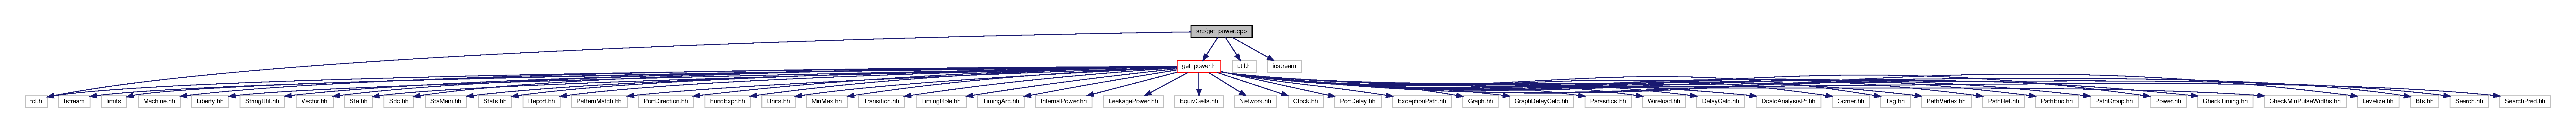
\includegraphics[width=350pt]{get__power_8cpp__incl}
\end{center}
\end{figure}

\hypertarget{get__power_8h}{}\section{src/get\+\_\+power.h File Reference}
\label{get__power_8h}\index{src/get\+\_\+power.\+h@{src/get\+\_\+power.\+h}}
{\ttfamily \#include $<$fstream$>$}\newline
{\ttfamily \#include $<$tcl.\+h$>$}\newline
{\ttfamily \#include $<$limits$>$}\newline
{\ttfamily \#include \char`\"{}Machine.\+hh\char`\"{}}\newline
{\ttfamily \#include \char`\"{}Liberty.\+hh\char`\"{}}\newline
{\ttfamily \#include \char`\"{}String\+Util.\+hh\char`\"{}}\newline
{\ttfamily \#include \char`\"{}Vector.\+hh\char`\"{}}\newline
{\ttfamily \#include \char`\"{}Sta.\+hh\char`\"{}}\newline
{\ttfamily \#include \char`\"{}Sdc.\+hh\char`\"{}}\newline
{\ttfamily \#include \char`\"{}Sta\+Main.\+hh\char`\"{}}\newline
{\ttfamily \#include \char`\"{}Stats.\+hh\char`\"{}}\newline
{\ttfamily \#include \char`\"{}Report.\+hh\char`\"{}}\newline
{\ttfamily \#include \char`\"{}Pattern\+Match.\+hh\char`\"{}}\newline
{\ttfamily \#include \char`\"{}Port\+Direction.\+hh\char`\"{}}\newline
{\ttfamily \#include \char`\"{}Func\+Expr.\+hh\char`\"{}}\newline
{\ttfamily \#include \char`\"{}Units.\+hh\char`\"{}}\newline
{\ttfamily \#include \char`\"{}Min\+Max.\+hh\char`\"{}}\newline
{\ttfamily \#include \char`\"{}Transition.\+hh\char`\"{}}\newline
{\ttfamily \#include \char`\"{}Timing\+Role.\+hh\char`\"{}}\newline
{\ttfamily \#include \char`\"{}Timing\+Arc.\+hh\char`\"{}}\newline
{\ttfamily \#include \char`\"{}Internal\+Power.\+hh\char`\"{}}\newline
{\ttfamily \#include \char`\"{}Leakage\+Power.\+hh\char`\"{}}\newline
{\ttfamily \#include \char`\"{}Equiv\+Cells.\+hh\char`\"{}}\newline
{\ttfamily \#include \char`\"{}Network.\+hh\char`\"{}}\newline
{\ttfamily \#include \char`\"{}Clock.\+hh\char`\"{}}\newline
{\ttfamily \#include \char`\"{}Port\+Delay.\+hh\char`\"{}}\newline
{\ttfamily \#include \char`\"{}Exception\+Path.\+hh\char`\"{}}\newline
{\ttfamily \#include \char`\"{}Graph.\+hh\char`\"{}}\newline
{\ttfamily \#include \char`\"{}Graph\+Delay\+Calc.\+hh\char`\"{}}\newline
{\ttfamily \#include \char`\"{}Parasitics.\+hh\char`\"{}}\newline
{\ttfamily \#include \char`\"{}Wireload.\+hh\char`\"{}}\newline
{\ttfamily \#include \char`\"{}Delay\+Calc.\+hh\char`\"{}}\newline
{\ttfamily \#include \char`\"{}Dcalc\+Analysis\+Pt.\+hh\char`\"{}}\newline
{\ttfamily \#include \char`\"{}Corner.\+hh\char`\"{}}\newline
{\ttfamily \#include \char`\"{}Tag.\+hh\char`\"{}}\newline
{\ttfamily \#include \char`\"{}Path\+Vertex.\+hh\char`\"{}}\newline
{\ttfamily \#include \char`\"{}Path\+Ref.\+hh\char`\"{}}\newline
{\ttfamily \#include \char`\"{}Path\+End.\+hh\char`\"{}}\newline
{\ttfamily \#include \char`\"{}Path\+Group.\+hh\char`\"{}}\newline
{\ttfamily \#include \char`\"{}Power.\+hh\char`\"{}}\newline
{\ttfamily \#include \char`\"{}Check\+Timing.\+hh\char`\"{}}\newline
{\ttfamily \#include \char`\"{}Check\+Min\+Pulse\+Widths.\+hh\char`\"{}}\newline
{\ttfamily \#include \char`\"{}Levelize.\+hh\char`\"{}}\newline
{\ttfamily \#include \char`\"{}Bfs.\+hh\char`\"{}}\newline
{\ttfamily \#include \char`\"{}Search.\+hh\char`\"{}}\newline
{\ttfamily \#include \char`\"{}Search\+Pred.\+hh\char`\"{}}\newline
{\ttfamily \#include \char`\"{}Path\+Analysis\+Pt.\+hh\char`\"{}}\newline
{\ttfamily \#include \char`\"{}Disallow\+Copy\+Assign.\+hh\char`\"{}}\newline
{\ttfamily \#include \char`\"{}Debug.\+hh\char`\"{}}\newline
{\ttfamily \#include \char`\"{}Error.\+hh\char`\"{}}\newline
{\ttfamily \#include \char`\"{}Verilog\+Namespace.\+hh\char`\"{}}\newline
{\ttfamily \#include \char`\"{}Verilog\+Reader.\+hh\char`\"{}}\newline
{\ttfamily \#include \char`\"{}Check\+Min\+Periods.\+hh\char`\"{}}\newline
{\ttfamily \#include \char`\"{}Check\+Max\+Skews.\+hh\char`\"{}}\newline
{\ttfamily \#include \char`\"{}Path\+Expanded.\+hh\char`\"{}}\newline
{\ttfamily \#include \char`\"{}Latches.\+hh\char`\"{}}\newline
{\ttfamily \#include \char`\"{}Report\+Path.\+hh\char`\"{}}\newline
{\ttfamily \#include \char`\"{}Visit\+Path\+Group\+Vertices.\+hh\char`\"{}}\newline
{\ttfamily \#include \char`\"{}Worst\+Slack.\+hh\char`\"{}}\newline
{\ttfamily \#include \char`\"{}Parasitics\+Class.\+hh\char`\"{}}\newline
{\ttfamily \#include \char`\"{}Parse\+Bus.\+hh\char`\"{}}\newline
This graph shows which files directly or indirectly include this file\+:\nopagebreak
\begin{figure}[H]
\begin{center}
\leavevmode
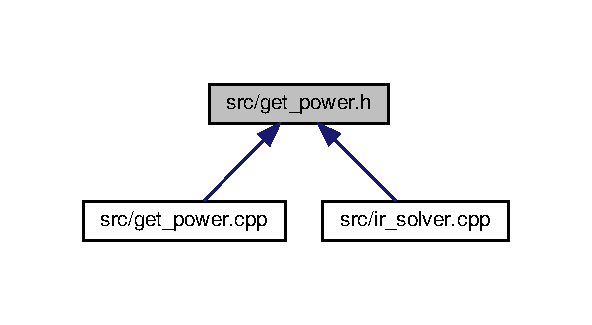
\includegraphics[width=284pt]{get__power_8h__dep__incl}
\end{center}
\end{figure}
\subsection*{Data Structures}
\begin{DoxyCompactItemize}
\item 
class \hyperlink{classPowerInst}{Power\+Inst}
\begin{DoxyCompactList}\small\item\em Calculates the power per instance using Open\+S\+TA. \end{DoxyCompactList}\end{DoxyCompactItemize}
\subsection*{Namespaces}
\begin{DoxyCompactItemize}
\item 
 \hyperlink{namespacesta}{sta}
\end{DoxyCompactItemize}
\subsection*{Macros}
\begin{DoxyCompactItemize}
\item 
\#define \hyperlink{get__power_8h_a58c98f6e8fc5d32aa3723dda4522fa00}{\+\_\+\+\_\+\+I\+R\+S\+O\+L\+V\+E\+R\+\_\+\+Power\+\_\+\+\_\+}~0
\end{DoxyCompactItemize}
\subsection*{Functions}
\begin{DoxyCompactItemize}
\item 
int \hyperlink{get__power_8h_a469736659db25c005ebaa45f3b0e1244}{Sta\+\_\+\+Init} (Tcl\+\_\+\+Interp $\ast$interp)
\end{DoxyCompactItemize}
\subsection*{Variables}
\begin{DoxyCompactItemize}
\item 
const char $\ast$ \hyperlink{namespacesta_a25423e815a38020350ff9ec056668087}{sta\+::tcl\+\_\+inits} \mbox{[}$\,$\mbox{]}
\end{DoxyCompactItemize}


\subsection{Macro Definition Documentation}
\mbox{\Hypertarget{get__power_8h_a58c98f6e8fc5d32aa3723dda4522fa00}\label{get__power_8h_a58c98f6e8fc5d32aa3723dda4522fa00}} 
\index{get\+\_\+power.\+h@{get\+\_\+power.\+h}!\+\_\+\+\_\+\+I\+R\+S\+O\+L\+V\+E\+R\+\_\+\+Power\+\_\+\+\_\+@{\+\_\+\+\_\+\+I\+R\+S\+O\+L\+V\+E\+R\+\_\+\+Power\+\_\+\+\_\+}}
\index{\+\_\+\+\_\+\+I\+R\+S\+O\+L\+V\+E\+R\+\_\+\+Power\+\_\+\+\_\+@{\+\_\+\+\_\+\+I\+R\+S\+O\+L\+V\+E\+R\+\_\+\+Power\+\_\+\+\_\+}!get\+\_\+power.\+h@{get\+\_\+power.\+h}}
\subsubsection{\texorpdfstring{\+\_\+\+\_\+\+I\+R\+S\+O\+L\+V\+E\+R\+\_\+\+Power\+\_\+\+\_\+}{\_\_IRSOLVER\_Power\_\_}}
{\footnotesize\ttfamily \#define \+\_\+\+\_\+\+I\+R\+S\+O\+L\+V\+E\+R\+\_\+\+Power\+\_\+\+\_\+~0}



\subsection{Function Documentation}
\mbox{\Hypertarget{get__power_8h_a469736659db25c005ebaa45f3b0e1244}\label{get__power_8h_a469736659db25c005ebaa45f3b0e1244}} 
\index{get\+\_\+power.\+h@{get\+\_\+power.\+h}!Sta\+\_\+\+Init@{Sta\+\_\+\+Init}}
\index{Sta\+\_\+\+Init@{Sta\+\_\+\+Init}!get\+\_\+power.\+h@{get\+\_\+power.\+h}}
\subsubsection{\texorpdfstring{Sta\+\_\+\+Init()}{Sta\_Init()}}
{\footnotesize\ttfamily int Sta\+\_\+\+Init (\begin{DoxyParamCaption}\item[{Tcl\+\_\+\+Interp $\ast$}]{interp }\end{DoxyParamCaption})}


\hypertarget{gmat_8cpp}{}\section{src/gmat.cpp File Reference}
\label{gmat_8cpp}\index{src/gmat.\+cpp@{src/gmat.\+cpp}}
{\ttfamily \#include $<$vector$>$}\newline
{\ttfamily \#include $<$iostream$>$}\newline
{\ttfamily \#include \char`\"{}gmat.\+h\char`\"{}}\newline
{\ttfamily \#include \char`\"{}node.\+h\char`\"{}}\newline
Include dependency graph for gmat.\+cpp\+:\nopagebreak
\begin{figure}[H]
\begin{center}
\leavevmode
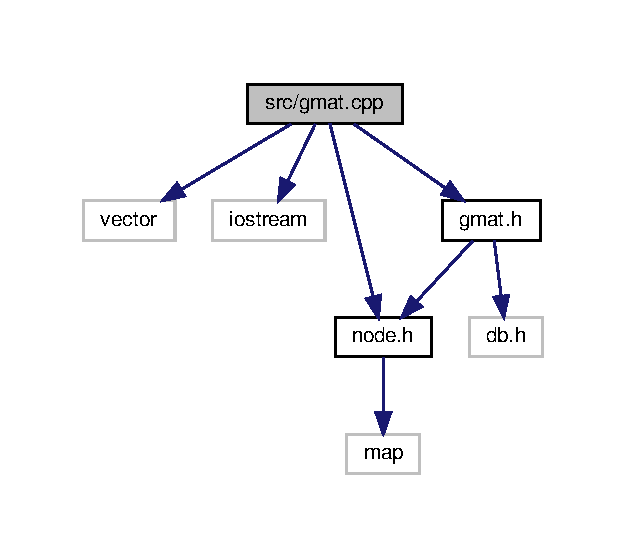
\includegraphics[width=301pt]{gmat_8cpp__incl}
\end{center}
\end{figure}

\hypertarget{gmat_8h}{}\section{src/gmat.h File Reference}
\label{gmat_8h}\index{src/gmat.\+h@{src/gmat.\+h}}
{\ttfamily \#include \char`\"{}node.\+h\char`\"{}}\newline
{\ttfamily \#include \char`\"{}db.\+h\char`\"{}}\newline
Include dependency graph for gmat.\+h\+:\nopagebreak
\begin{figure}[H]
\begin{center}
\leavevmode
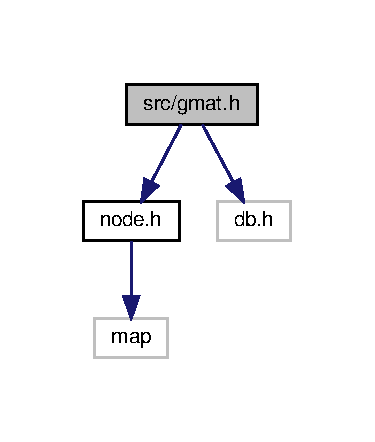
\includegraphics[width=180pt]{gmat_8h__incl}
\end{center}
\end{figure}
This graph shows which files directly or indirectly include this file\+:\nopagebreak
\begin{figure}[H]
\begin{center}
\leavevmode
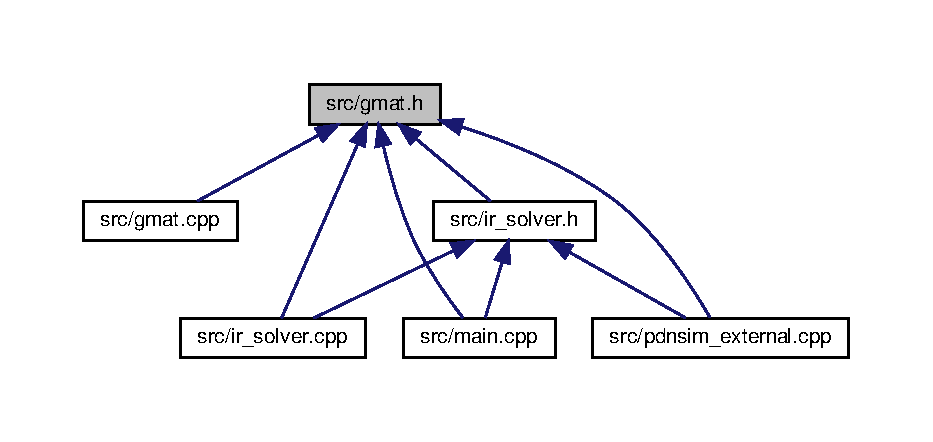
\includegraphics[width=350pt]{gmat_8h__dep__incl}
\end{center}
\end{figure}
\subsection*{Data Structures}
\begin{DoxyCompactItemize}
\item 
class \hyperlink{classGMat}{G\+Mat}
\begin{DoxyCompactList}\small\item\em G matrix class. \end{DoxyCompactList}\end{DoxyCompactItemize}
\subsection*{Typedefs}
\begin{DoxyCompactItemize}
\item 
typedef std\+::map$<$ int, std\+::map$<$ int, \hyperlink{classNode}{Node} $\ast$ $>$ $>$ \hyperlink{gmat_8h_a25a6eb13135bc88c32c443ba735c8a14}{Node\+Map}
\begin{DoxyCompactList}\small\item\em Global variable which holds the G matrix. \end{DoxyCompactList}\end{DoxyCompactItemize}


\subsection{Typedef Documentation}
\mbox{\Hypertarget{gmat_8h_a25a6eb13135bc88c32c443ba735c8a14}\label{gmat_8h_a25a6eb13135bc88c32c443ba735c8a14}} 
\index{gmat.\+h@{gmat.\+h}!Node\+Map@{Node\+Map}}
\index{Node\+Map@{Node\+Map}!gmat.\+h@{gmat.\+h}}
\subsubsection{\texorpdfstring{Node\+Map}{NodeMap}}
{\footnotesize\ttfamily typedef std\+::map$<$int, std\+::map$<$int, \hyperlink{classNode}{Node}$\ast$$>$ $>$ \hyperlink{gmat_8h_a25a6eb13135bc88c32c443ba735c8a14}{Node\+Map}}



Global variable which holds the G matrix. 

Three dimensions with layer number,x location, and y location. Holds a pointer to the node of the power grid. 
\hypertarget{ir__solver_8cpp}{}\section{src/ir\+\_\+solver.cpp File Reference}
\label{ir__solver_8cpp}\index{src/ir\+\_\+solver.\+cpp@{src/ir\+\_\+solver.\+cpp}}
{\ttfamily \#include $<$vector$>$}\newline
{\ttfamily \#include $<$math.\+h$>$}\newline
{\ttfamily \#include $<$cmath$>$}\newline
{\ttfamily \#include $<$iostream$>$}\newline
{\ttfamily \#include $<$stdlib.\+h$>$}\newline
{\ttfamily \#include $<$map$>$}\newline
{\ttfamily \#include $<$fstream$>$}\newline
{\ttfamily \#include $<$iomanip$>$}\newline
{\ttfamily \#include $<$time.\+h$>$}\newline
{\ttfamily \#include $<$sstream$>$}\newline
{\ttfamily \#include $<$iterator$>$}\newline
{\ttfamily \#include $<$string$>$}\newline
{\ttfamily \#include \char`\"{}slu\+\_\+ddefs.\+h\char`\"{}}\newline
{\ttfamily \#include \char`\"{}db.\+h\char`\"{}}\newline
{\ttfamily \#include \char`\"{}ir\+\_\+solver.\+h\char`\"{}}\newline
{\ttfamily \#include \char`\"{}node.\+h\char`\"{}}\newline
{\ttfamily \#include \char`\"{}gmat.\+h\char`\"{}}\newline
{\ttfamily \#include \char`\"{}get\+\_\+power.\+h\char`\"{}}\newline
Include dependency graph for ir\+\_\+solver.\+cpp\+:\nopagebreak
\begin{figure}[H]
\begin{center}
\leavevmode
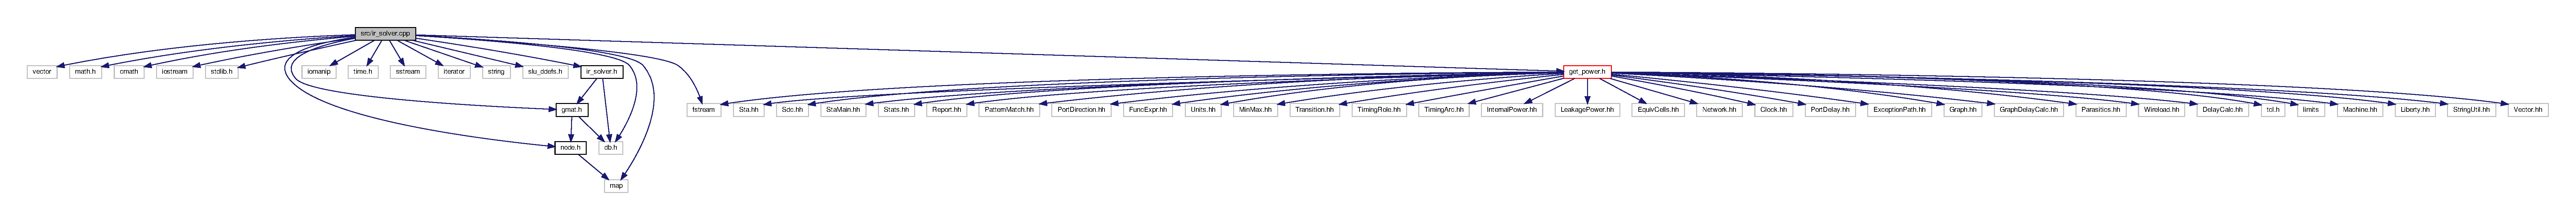
\includegraphics[width=350pt]{ir__solver_8cpp__incl}
\end{center}
\end{figure}

\hypertarget{ir__solver_8h}{}\section{src/ir\+\_\+solver.h File Reference}
\label{ir__solver_8h}\index{src/ir\+\_\+solver.\+h@{src/ir\+\_\+solver.\+h}}
{\ttfamily \#include \char`\"{}gmat.\+h\char`\"{}}\newline
{\ttfamily \#include \char`\"{}db.\+h\char`\"{}}\newline
Include dependency graph for ir\+\_\+solver.\+h\+:\nopagebreak
\begin{figure}[H]
\begin{center}
\leavevmode
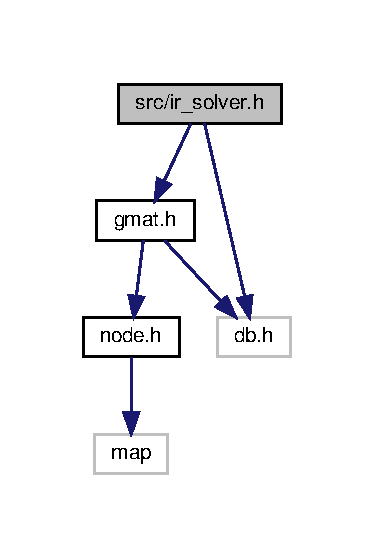
\includegraphics[width=180pt]{ir__solver_8h__incl}
\end{center}
\end{figure}
This graph shows which files directly or indirectly include this file\+:\nopagebreak
\begin{figure}[H]
\begin{center}
\leavevmode
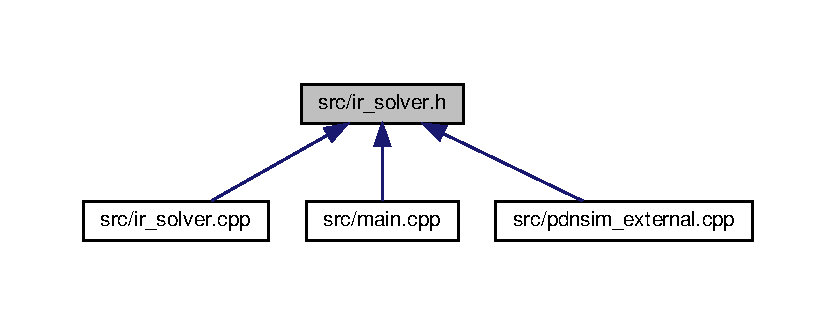
\includegraphics[width=350pt]{ir__solver_8h__dep__incl}
\end{center}
\end{figure}
\subsection*{Data Structures}
\begin{DoxyCompactItemize}
\item 
class \hyperlink{classIRSolver}{I\+R\+Solver}
\begin{DoxyCompactList}\small\item\em Class for IR solver. \end{DoxyCompactList}\end{DoxyCompactItemize}

\hypertarget{main_8cpp}{}\section{src/main.cpp File Reference}
\label{main_8cpp}\index{src/main.\+cpp@{src/main.\+cpp}}
{\ttfamily \#include \char`\"{}pdnsim\+\_\+external.\+h\char`\"{}}\newline
{\ttfamily \#include $<$tcl.\+h$>$}\newline
{\ttfamily \#include $<$fstream$>$}\newline
{\ttfamily \#include $<$iostream$>$}\newline
{\ttfamily \#include $<$iomanip$>$}\newline
{\ttfamily \#include $<$sstream$>$}\newline
{\ttfamily \#include \char`\"{}db.\+h\char`\"{}}\newline
{\ttfamily \#include \char`\"{}ir\+\_\+solver.\+h\char`\"{}}\newline
{\ttfamily \#include $<$string$>$}\newline
{\ttfamily \#include $<$vector$>$}\newline
{\ttfamily \#include \char`\"{}gmat.\+h\char`\"{}}\newline
{\ttfamily \#include \char`\"{}node.\+h\char`\"{}}\newline
{\ttfamily \#include \char`\"{}parameters.\+h\char`\"{}}\newline
Include dependency graph for main.\+cpp\+:\nopagebreak
\begin{figure}[H]
\begin{center}
\leavevmode
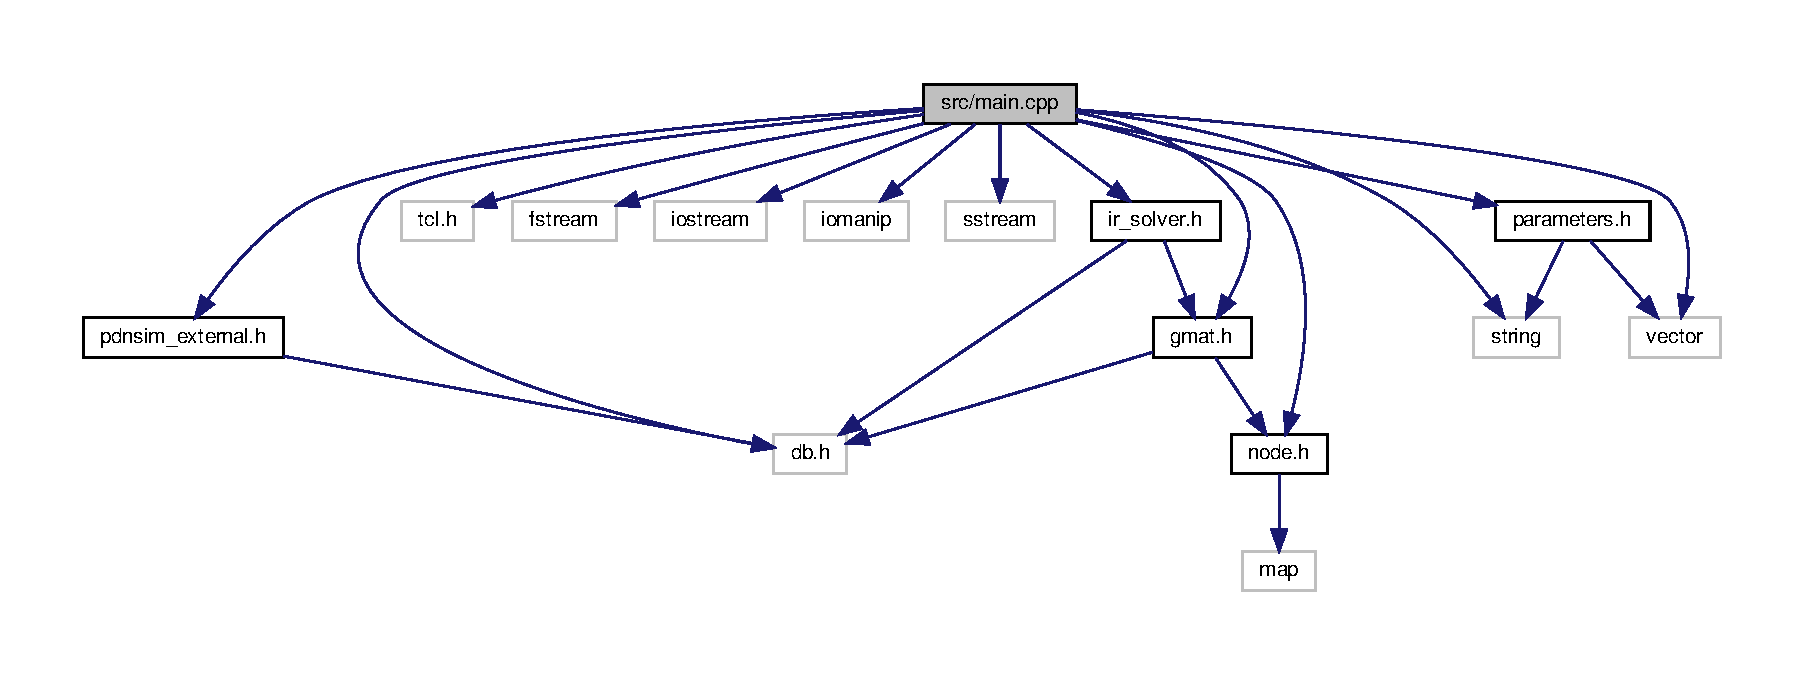
\includegraphics[width=350pt]{main_8cpp__incl}
\end{center}
\end{figure}
\subsection*{Functions}
\begin{DoxyCompactItemize}
\item 
int \hyperlink{main_8cpp_ab466f3e64539d11e9348387c4ccc7d59}{Irsolver\+\_\+\+Init} (Tcl\+\_\+\+Interp $\ast$interp)
\item 
int \hyperlink{main_8cpp_a45ebeb0bf1dca4a0fa522704007aac66}{P\+D\+N\+Sim\+Tcl\+App\+Init} (Tcl\+\_\+\+Interp $\ast$interp)
\item 
int \hyperlink{main_8cpp_adf8b34a2c8b7df30f7140692b3187a8a}{pdn\+\_\+sim} (\hyperlink{classParameters}{Parameters} $\ast$parms\+To\+P\+D\+N\+Sim)
\item 
int \hyperlink{main_8cpp_a3c04138a5bfe5d72780bb7e82a18e627}{main} (int argc, char $\ast$$\ast$argv)
\end{DoxyCompactItemize}


\subsection{Function Documentation}
\mbox{\Hypertarget{main_8cpp_ab466f3e64539d11e9348387c4ccc7d59}\label{main_8cpp_ab466f3e64539d11e9348387c4ccc7d59}} 
\index{main.\+cpp@{main.\+cpp}!Irsolver\+\_\+\+Init@{Irsolver\+\_\+\+Init}}
\index{Irsolver\+\_\+\+Init@{Irsolver\+\_\+\+Init}!main.\+cpp@{main.\+cpp}}
\subsubsection{\texorpdfstring{Irsolver\+\_\+\+Init()}{Irsolver\_Init()}}
{\footnotesize\ttfamily int Irsolver\+\_\+\+Init (\begin{DoxyParamCaption}\item[{Tcl\+\_\+\+Interp $\ast$}]{interp }\end{DoxyParamCaption})}

\mbox{\Hypertarget{main_8cpp_a3c04138a5bfe5d72780bb7e82a18e627}\label{main_8cpp_a3c04138a5bfe5d72780bb7e82a18e627}} 
\index{main.\+cpp@{main.\+cpp}!main@{main}}
\index{main@{main}!main.\+cpp@{main.\+cpp}}
\subsubsection{\texorpdfstring{main()}{main()}}
{\footnotesize\ttfamily int main (\begin{DoxyParamCaption}\item[{int}]{argc,  }\item[{char $\ast$$\ast$}]{argv }\end{DoxyParamCaption})}

\mbox{\Hypertarget{main_8cpp_adf8b34a2c8b7df30f7140692b3187a8a}\label{main_8cpp_adf8b34a2c8b7df30f7140692b3187a8a}} 
\index{main.\+cpp@{main.\+cpp}!pdn\+\_\+sim@{pdn\+\_\+sim}}
\index{pdn\+\_\+sim@{pdn\+\_\+sim}!main.\+cpp@{main.\+cpp}}
\subsubsection{\texorpdfstring{pdn\+\_\+sim()}{pdn\_sim()}}
{\footnotesize\ttfamily int pdn\+\_\+sim (\begin{DoxyParamCaption}\item[{\hyperlink{classParameters}{Parameters} $\ast$}]{parms\+To\+P\+D\+N\+Sim }\end{DoxyParamCaption})}

\mbox{\Hypertarget{main_8cpp_a45ebeb0bf1dca4a0fa522704007aac66}\label{main_8cpp_a45ebeb0bf1dca4a0fa522704007aac66}} 
\index{main.\+cpp@{main.\+cpp}!P\+D\+N\+Sim\+Tcl\+App\+Init@{P\+D\+N\+Sim\+Tcl\+App\+Init}}
\index{P\+D\+N\+Sim\+Tcl\+App\+Init@{P\+D\+N\+Sim\+Tcl\+App\+Init}!main.\+cpp@{main.\+cpp}}
\subsubsection{\texorpdfstring{P\+D\+N\+Sim\+Tcl\+App\+Init()}{PDNSimTclAppInit()}}
{\footnotesize\ttfamily int P\+D\+N\+Sim\+Tcl\+App\+Init (\begin{DoxyParamCaption}\item[{Tcl\+\_\+\+Interp $\ast$}]{interp }\end{DoxyParamCaption})}


\hypertarget{node_8cpp}{}\section{src/node.cpp File Reference}
\label{node_8cpp}\index{src/node.\+cpp@{src/node.\+cpp}}
{\ttfamily \#include $<$vector$>$}\newline
{\ttfamily \#include $<$iostream$>$}\newline
{\ttfamily \#include \char`\"{}node.\+h\char`\"{}}\newline
Include dependency graph for node.\+cpp\+:\nopagebreak
\begin{figure}[H]
\begin{center}
\leavevmode
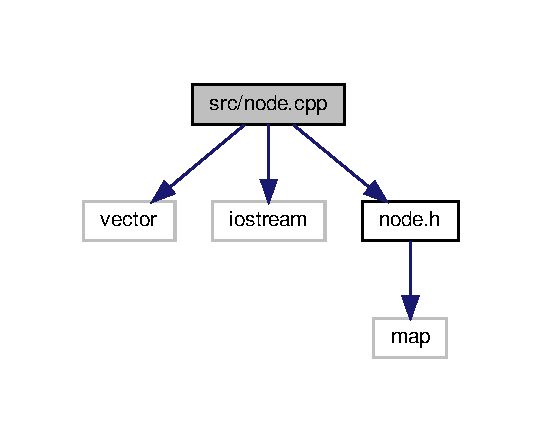
\includegraphics[width=260pt]{node_8cpp__incl}
\end{center}
\end{figure}

\hypertarget{node_8h}{}\section{src/node.h File Reference}
\label{node_8h}\index{src/node.\+h@{src/node.\+h}}
{\ttfamily \#include $<$map$>$}\newline
Include dependency graph for node.\+h\+:\nopagebreak
\begin{figure}[H]
\begin{center}
\leavevmode
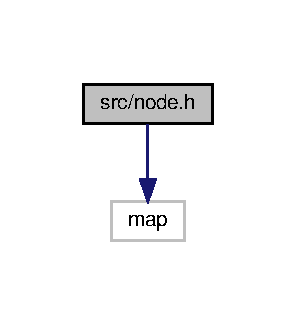
\includegraphics[width=142pt]{node_8h__incl}
\end{center}
\end{figure}
This graph shows which files directly or indirectly include this file\+:\nopagebreak
\begin{figure}[H]
\begin{center}
\leavevmode
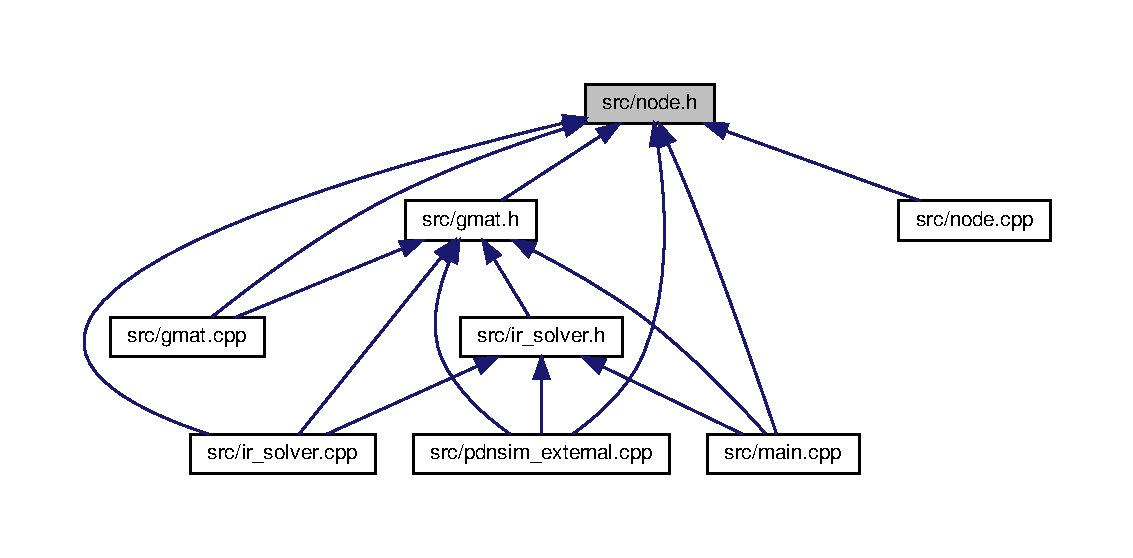
\includegraphics[width=350pt]{node_8h__dep__incl}
\end{center}
\end{figure}
\subsection*{Data Structures}
\begin{DoxyCompactItemize}
\item 
struct \hyperlink{structDokMatrix}{Dok\+Matrix}
\begin{DoxyCompactList}\small\item\em Data structure for the Dictionary of Keys Matrix. \end{DoxyCompactList}\item 
struct \hyperlink{structCscMatrix}{Csc\+Matrix}
\begin{DoxyCompactList}\small\item\em Data structure for the Compressed Sparse Column Matrix. \end{DoxyCompactList}\item 
class \hyperlink{classNode}{Node}
\begin{DoxyCompactList}\small\item\em \hyperlink{classNode}{Node} class which stores the properties of the node of the P\+DN. \end{DoxyCompactList}\end{DoxyCompactItemize}
\subsection*{Typedefs}
\begin{DoxyCompactItemize}
\item 
typedef std\+::pair$<$ int, int $>$ \hyperlink{node_8h_a8457e7507941d06122aaf5c4ac260995}{Node\+Loc}
\item 
typedef std\+::pair$<$ int, int $>$ \hyperlink{node_8h_acf0ff4a0bb7e0c9b5900382cbd2aa614}{B\+Box}
\item 
typedef int \hyperlink{node_8h_a5b622fe4354316a2f349615d150ae998}{Node\+Idx}
\item 
typedef std\+::pair$<$ \hyperlink{node_8h_a5b622fe4354316a2f349615d150ae998}{Node\+Idx}, \hyperlink{node_8h_a5b622fe4354316a2f349615d150ae998}{Node\+Idx} $>$ \hyperlink{node_8h_aaffe095b1e5d88040e6ca3976576fccf}{G\+Mat\+Loc}
\end{DoxyCompactItemize}


\subsection{Typedef Documentation}
\mbox{\Hypertarget{node_8h_acf0ff4a0bb7e0c9b5900382cbd2aa614}\label{node_8h_acf0ff4a0bb7e0c9b5900382cbd2aa614}} 
\index{node.\+h@{node.\+h}!B\+Box@{B\+Box}}
\index{B\+Box@{B\+Box}!node.\+h@{node.\+h}}
\subsubsection{\texorpdfstring{B\+Box}{BBox}}
{\footnotesize\ttfamily typedef std\+::pair$<$int, int$>$ \hyperlink{node_8h_acf0ff4a0bb7e0c9b5900382cbd2aa614}{B\+Box}}

\mbox{\Hypertarget{node_8h_aaffe095b1e5d88040e6ca3976576fccf}\label{node_8h_aaffe095b1e5d88040e6ca3976576fccf}} 
\index{node.\+h@{node.\+h}!G\+Mat\+Loc@{G\+Mat\+Loc}}
\index{G\+Mat\+Loc@{G\+Mat\+Loc}!node.\+h@{node.\+h}}
\subsubsection{\texorpdfstring{G\+Mat\+Loc}{GMatLoc}}
{\footnotesize\ttfamily typedef std\+::pair$<$\hyperlink{node_8h_a5b622fe4354316a2f349615d150ae998}{Node\+Idx}, \hyperlink{node_8h_a5b622fe4354316a2f349615d150ae998}{Node\+Idx}$>$ \hyperlink{node_8h_aaffe095b1e5d88040e6ca3976576fccf}{G\+Mat\+Loc}}

\mbox{\Hypertarget{node_8h_a5b622fe4354316a2f349615d150ae998}\label{node_8h_a5b622fe4354316a2f349615d150ae998}} 
\index{node.\+h@{node.\+h}!Node\+Idx@{Node\+Idx}}
\index{Node\+Idx@{Node\+Idx}!node.\+h@{node.\+h}}
\subsubsection{\texorpdfstring{Node\+Idx}{NodeIdx}}
{\footnotesize\ttfamily typedef int \hyperlink{node_8h_a5b622fe4354316a2f349615d150ae998}{Node\+Idx}}

\mbox{\Hypertarget{node_8h_a8457e7507941d06122aaf5c4ac260995}\label{node_8h_a8457e7507941d06122aaf5c4ac260995}} 
\index{node.\+h@{node.\+h}!Node\+Loc@{Node\+Loc}}
\index{Node\+Loc@{Node\+Loc}!node.\+h@{node.\+h}}
\subsubsection{\texorpdfstring{Node\+Loc}{NodeLoc}}
{\footnotesize\ttfamily typedef std\+::pair$<$int, int$>$ \hyperlink{node_8h_a8457e7507941d06122aaf5c4ac260995}{Node\+Loc}}


\hypertarget{parameters_8cpp}{}\section{src/parameters.cpp File Reference}
\label{parameters_8cpp}\index{src/parameters.\+cpp@{src/parameters.\+cpp}}
{\ttfamily \#include \char`\"{}parameters.\+h\char`\"{}}\newline
{\ttfamily \#include $<$iostream$>$}\newline
{\ttfamily \#include $<$iomanip$>$}\newline
{\ttfamily \#include $<$boost/program\+\_\+options.\+hpp$>$}\newline
Include dependency graph for parameters.\+cpp\+:\nopagebreak
\begin{figure}[H]
\begin{center}
\leavevmode
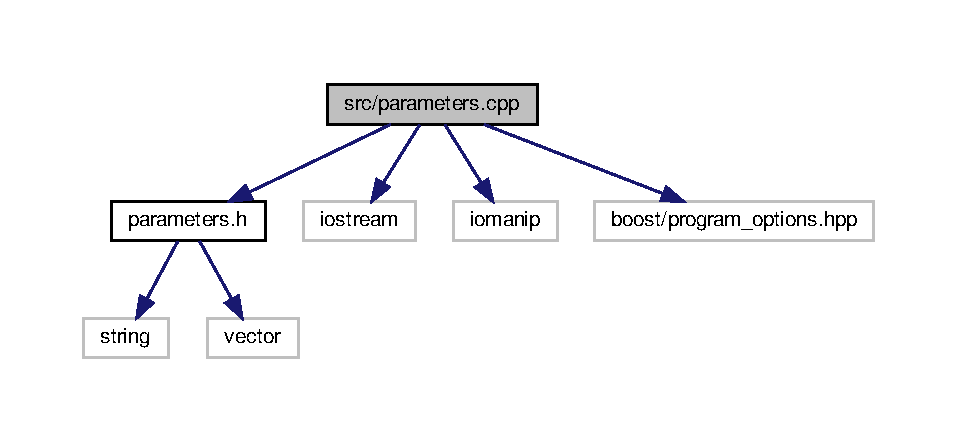
\includegraphics[width=350pt]{parameters_8cpp__incl}
\end{center}
\end{figure}

\hypertarget{parameters_8h}{}\section{src/parameters.h File Reference}
\label{parameters_8h}\index{src/parameters.\+h@{src/parameters.\+h}}
{\ttfamily \#include $<$string$>$}\newline
{\ttfamily \#include $<$vector$>$}\newline
Include dependency graph for parameters.\+h\+:\nopagebreak
\begin{figure}[H]
\begin{center}
\leavevmode
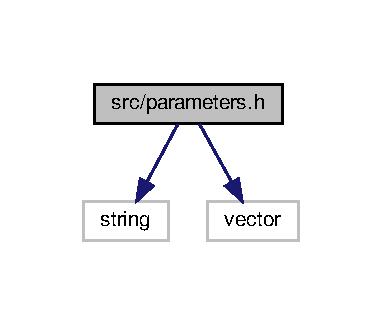
\includegraphics[width=184pt]{parameters_8h__incl}
\end{center}
\end{figure}
This graph shows which files directly or indirectly include this file\+:\nopagebreak
\begin{figure}[H]
\begin{center}
\leavevmode
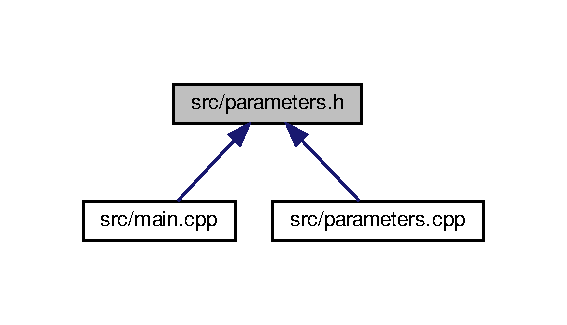
\includegraphics[width=272pt]{parameters_8h__dep__incl}
\end{center}
\end{figure}
\subsection*{Data Structures}
\begin{DoxyCompactItemize}
\item 
class \hyperlink{classParameters}{Parameters}
\end{DoxyCompactItemize}

\hypertarget{pdnsim__external_8cpp}{}\section{src/pdnsim\+\_\+external.cpp File Reference}
\label{pdnsim__external_8cpp}\index{src/pdnsim\+\_\+external.\+cpp@{src/pdnsim\+\_\+external.\+cpp}}
{\ttfamily \#include $<$vector$>$}\newline
{\ttfamily \#include $<$iostream$>$}\newline
{\ttfamily \#include $<$fstream$>$}\newline
{\ttfamily \#include $<$iomanip$>$}\newline
{\ttfamily \#include $<$sstream$>$}\newline
{\ttfamily \#include $<$string$>$}\newline
{\ttfamily \#include \char`\"{}pdnsim\+\_\+external.\+h\char`\"{}}\newline
{\ttfamily \#include \char`\"{}db.\+h\char`\"{}}\newline
{\ttfamily \#include \char`\"{}lefin.\+h\char`\"{}}\newline
{\ttfamily \#include \char`\"{}defin.\+h\char`\"{}}\newline
{\ttfamily \#include \char`\"{}gmat.\+h\char`\"{}}\newline
{\ttfamily \#include \char`\"{}ir\+\_\+solver.\+h\char`\"{}}\newline
{\ttfamily \#include \char`\"{}node.\+h\char`\"{}}\newline
Include dependency graph for pdnsim\+\_\+external.\+cpp\+:\nopagebreak
\begin{figure}[H]
\begin{center}
\leavevmode
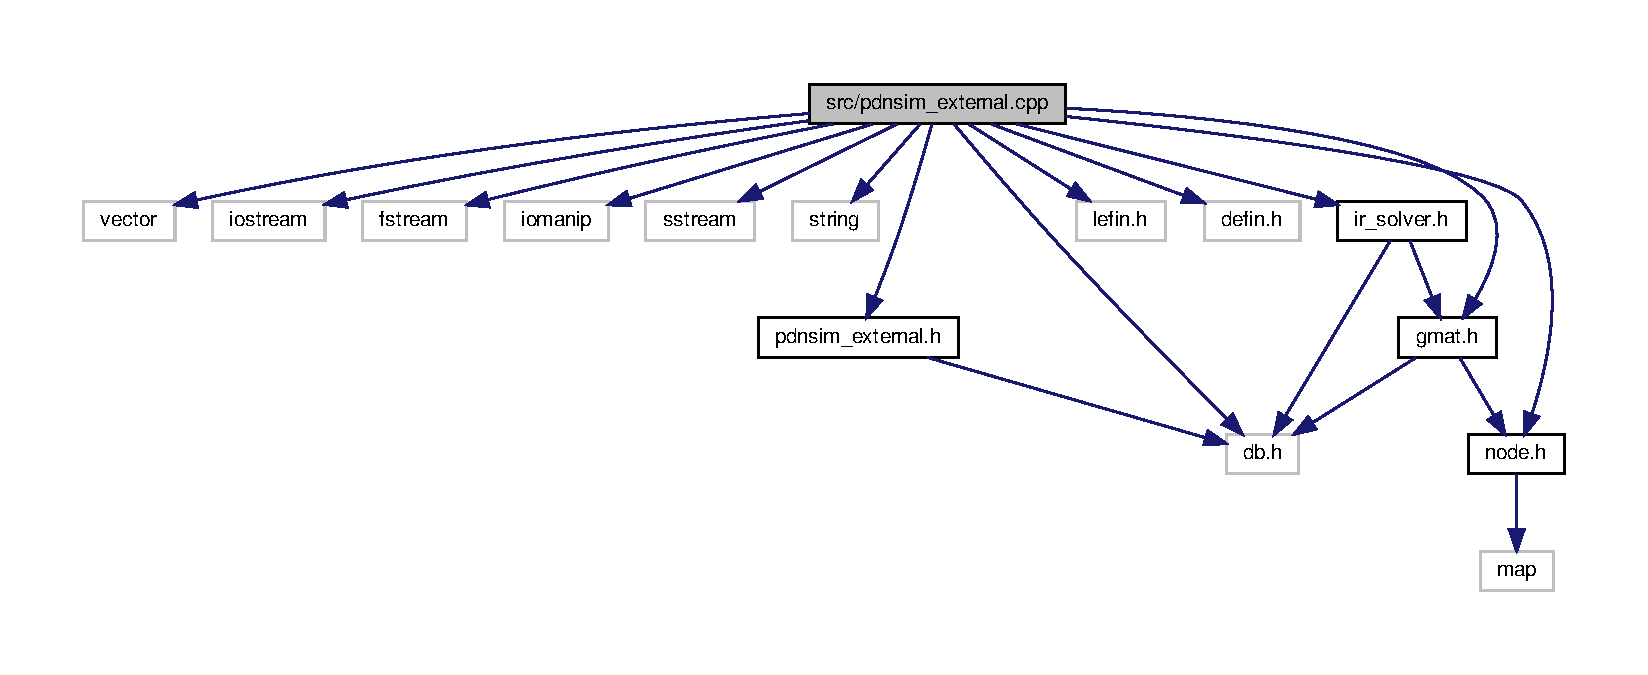
\includegraphics[width=350pt]{pdnsim__external_8cpp__incl}
\end{center}
\end{figure}

\hypertarget{pdnsim__external_8h}{}\section{src/pdnsim\+\_\+external.h File Reference}
\label{pdnsim__external_8h}\index{src/pdnsim\+\_\+external.\+h@{src/pdnsim\+\_\+external.\+h}}
{\ttfamily \#include \char`\"{}db.\+h\char`\"{}}\newline
Include dependency graph for pdnsim\+\_\+external.\+h\+:\nopagebreak
\begin{figure}[H]
\begin{center}
\leavevmode
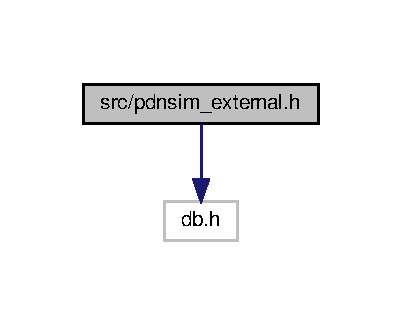
\includegraphics[width=193pt]{pdnsim__external_8h__incl}
\end{center}
\end{figure}
This graph shows which files directly or indirectly include this file\+:\nopagebreak
\begin{figure}[H]
\begin{center}
\leavevmode
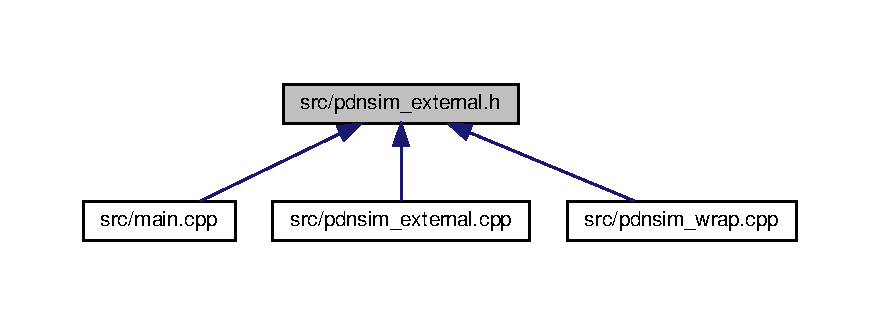
\includegraphics[width=350pt]{pdnsim__external_8h__dep__incl}
\end{center}
\end{figure}
\subsection*{Data Structures}
\begin{DoxyCompactItemize}
\item 
class \hyperlink{classPDNSim}{P\+D\+N\+Sim}
\end{DoxyCompactItemize}

\hypertarget{pdnsim__wrap_8cpp}{}\section{src/pdnsim\+\_\+wrap.cpp File Reference}
\label{pdnsim__wrap_8cpp}\index{src/pdnsim\+\_\+wrap.\+cpp@{src/pdnsim\+\_\+wrap.\+cpp}}
{\ttfamily \#include $<$stdio.\+h$>$}\newline
{\ttfamily \#include $<$tcl.\+h$>$}\newline
{\ttfamily \#include $<$errno.\+h$>$}\newline
{\ttfamily \#include $<$stdlib.\+h$>$}\newline
{\ttfamily \#include $<$stdarg.\+h$>$}\newline
{\ttfamily \#include $<$ctype.\+h$>$}\newline
{\ttfamily \#include $<$string.\+h$>$}\newline
{\ttfamily \#include \char`\"{}assert.\+h\char`\"{}}\newline
{\ttfamily \#include $<$stdexcept$>$}\newline
{\ttfamily \#include \char`\"{}pdnsim\+\_\+external.\+h\char`\"{}}\newline
{\ttfamily \#include $<$typeinfo$>$}\newline
{\ttfamily \#include $<$string$>$}\newline
{\ttfamily \#include $<$algorithm$>$}\newline
{\ttfamily \#include $<$vector$>$}\newline
{\ttfamily \#include $<$map$>$}\newline
{\ttfamily \#include $<$utility$>$}\newline
{\ttfamily \#include $<$limits.\+h$>$}\newline
Include dependency graph for pdnsim\+\_\+wrap.\+cpp\+:\nopagebreak
\begin{figure}[H]
\begin{center}
\leavevmode
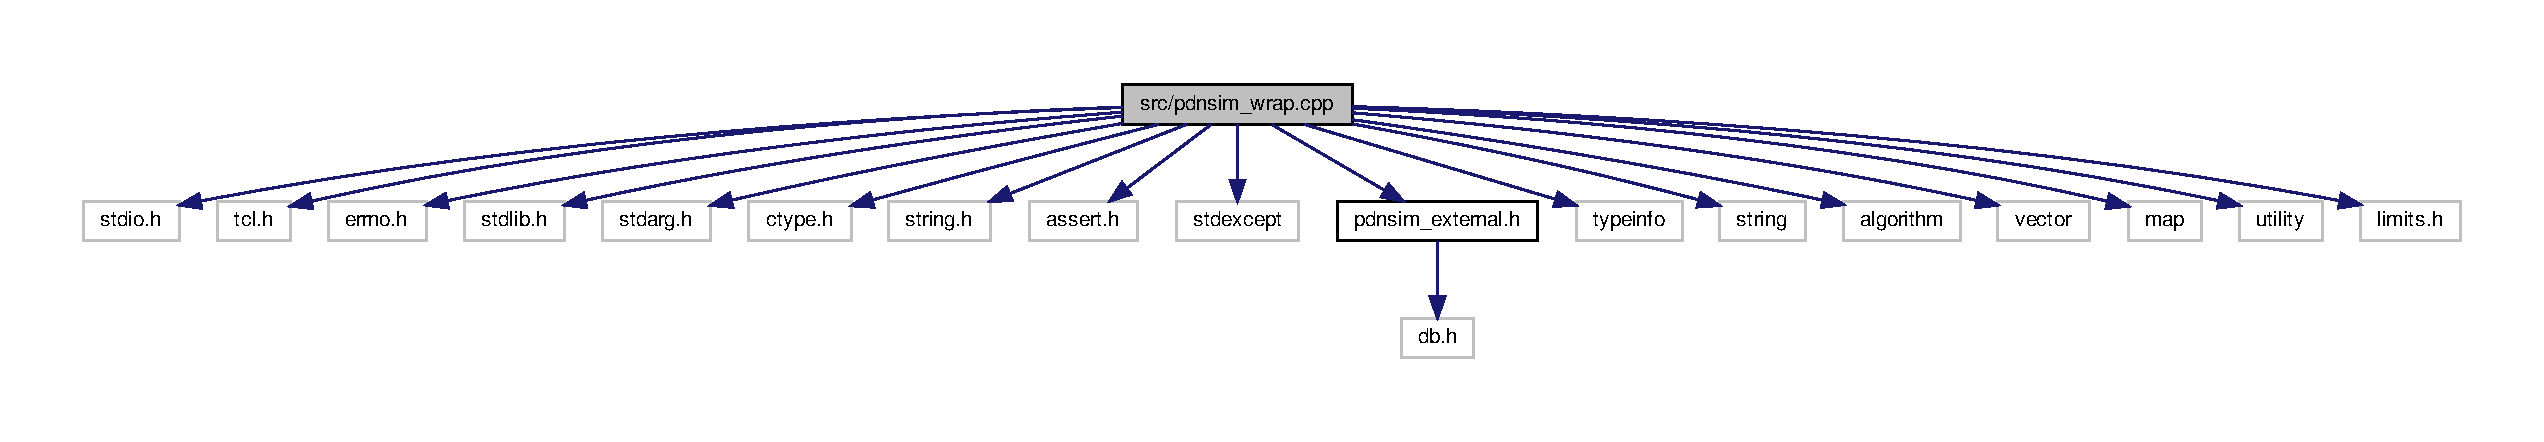
\includegraphics[width=350pt]{pdnsim__wrap_8cpp__incl}
\end{center}
\end{figure}
\subsection*{Data Structures}
\begin{DoxyCompactItemize}
\item 
struct \hyperlink{structswig__type__info}{swig\+\_\+type\+\_\+info}
\item 
struct \hyperlink{structswig__cast__info}{swig\+\_\+cast\+\_\+info}
\item 
struct \hyperlink{structswig__module__info}{swig\+\_\+module\+\_\+info}
\item 
struct \hyperlink{structswig__const__info}{swig\+\_\+const\+\_\+info}
\item 
struct \hyperlink{structswig__method}{swig\+\_\+method}
\item 
struct \hyperlink{structswig__attribute}{swig\+\_\+attribute}
\item 
struct \hyperlink{structswig__class}{swig\+\_\+class}
\item 
struct \hyperlink{structswig__instance}{swig\+\_\+instance}
\item 
struct \hyperlink{structswig__command__info}{swig\+\_\+command\+\_\+info}
\item 
struct \hyperlink{structswig__var__info}{swig\+\_\+var\+\_\+info}
\end{DoxyCompactItemize}
\subsection*{Macros}
\begin{DoxyCompactItemize}
\item 
\#define \hyperlink{pdnsim__wrap_8cpp_a6c2119ff2df29f6b0798d551d633c986}{S\+W\+I\+G\+T\+CL}
\item 
\#define \hyperlink{pdnsim__wrap_8cpp_a7e84031693895e512662f5b390c6d0e4}{S\+W\+I\+G\+T\+E\+M\+P\+L\+A\+T\+E\+D\+I\+S\+A\+M\+B\+I\+G\+U\+A\+T\+OR}
\item 
\#define \hyperlink{pdnsim__wrap_8cpp_a6d0a7c65b3712775e92c8bdb7acdd0ee}{S\+W\+I\+G\+I\+N\+L\+I\+NE}
\item 
\#define \hyperlink{pdnsim__wrap_8cpp_a6ee41cd160d397aa76668bf4db65e2d1}{S\+W\+I\+G\+U\+N\+U\+S\+ED}
\item 
\#define \hyperlink{pdnsim__wrap_8cpp_a6a54164d0685c632e7540c5ad32a453a}{S\+W\+I\+G\+U\+N\+U\+S\+E\+D\+P\+A\+RM}(p)~p \hyperlink{pdnsim__wrap_8cpp_a6ee41cd160d397aa76668bf4db65e2d1}{S\+W\+I\+G\+U\+N\+U\+S\+ED}
\item 
\#define \hyperlink{pdnsim__wrap_8cpp_a8f2319f775e5b9d5906c9ef25d9b819a}{S\+W\+I\+G\+I\+N\+T\+E\+RN}~static \hyperlink{pdnsim__wrap_8cpp_a6ee41cd160d397aa76668bf4db65e2d1}{S\+W\+I\+G\+U\+N\+U\+S\+ED}
\item 
\#define \hyperlink{pdnsim__wrap_8cpp_afc5b08bb3c3cd2e3fb2e34b775346153}{S\+W\+I\+G\+I\+N\+T\+E\+R\+N\+I\+N\+L\+I\+NE}~\hyperlink{pdnsim__wrap_8cpp_a8f2319f775e5b9d5906c9ef25d9b819a}{S\+W\+I\+G\+I\+N\+T\+E\+RN} \hyperlink{pdnsim__wrap_8cpp_a6d0a7c65b3712775e92c8bdb7acdd0ee}{S\+W\+I\+G\+I\+N\+L\+I\+NE}
\item 
\#define \hyperlink{pdnsim__wrap_8cpp_aea3c8b056dcc8c1ab93f6b825cd1371b}{S\+W\+I\+G\+E\+X\+P\+O\+RT}
\item 
\#define \hyperlink{pdnsim__wrap_8cpp_adcd6410456ea7a76147d3ad95b9bcb36}{S\+W\+I\+G\+S\+T\+D\+C\+A\+LL}
\item 
\#define \hyperlink{pdnsim__wrap_8cpp_a4895907de5539551925ab5c03ea05d28}{S\+W\+I\+G\+\_\+\+R\+U\+N\+T\+I\+M\+E\+\_\+\+V\+E\+R\+S\+I\+ON}~\char`\"{}4\char`\"{}
\item 
\#define \hyperlink{pdnsim__wrap_8cpp_ac619a84edecccb5e00c1b4a3180b8c3a}{S\+W\+I\+G\+\_\+\+T\+Y\+P\+E\+\_\+\+T\+A\+B\+L\+E\+\_\+\+N\+A\+ME}
\item 
\#define \hyperlink{pdnsim__wrap_8cpp_a42cd9c1d67d803040a3e78515945afcb}{S\+W\+I\+G\+R\+U\+N\+T\+I\+ME}~\hyperlink{pdnsim__wrap_8cpp_a8f2319f775e5b9d5906c9ef25d9b819a}{S\+W\+I\+G\+I\+N\+T\+E\+RN}
\item 
\#define \hyperlink{pdnsim__wrap_8cpp_affa7aa2bcce5bea24a20e5b184ae0533}{S\+W\+I\+G\+R\+U\+N\+T\+I\+M\+E\+I\+N\+L\+I\+NE}~\hyperlink{pdnsim__wrap_8cpp_a42cd9c1d67d803040a3e78515945afcb}{S\+W\+I\+G\+R\+U\+N\+T\+I\+ME} \hyperlink{pdnsim__wrap_8cpp_a6d0a7c65b3712775e92c8bdb7acdd0ee}{S\+W\+I\+G\+I\+N\+L\+I\+NE}
\item 
\#define \hyperlink{pdnsim__wrap_8cpp_a26324fcd1baceab72680dfec078da440}{S\+W\+I\+G\+\_\+\+B\+U\+F\+F\+E\+R\+\_\+\+S\+I\+ZE}~1024
\item 
\#define \hyperlink{pdnsim__wrap_8cpp_aa56139a289829795ed651d533826b65e}{S\+W\+I\+G\+\_\+\+P\+O\+I\+N\+T\+E\+R\+\_\+\+D\+I\+S\+O\+WN}~0x1
\item 
\#define \hyperlink{pdnsim__wrap_8cpp_ac8216459bfd45cbd2be36175ef6f1ccc}{S\+W\+I\+G\+\_\+\+C\+A\+S\+T\+\_\+\+N\+E\+W\+\_\+\+M\+E\+M\+O\+RY}~0x2
\item 
\#define \hyperlink{pdnsim__wrap_8cpp_a1a125b0e9c551bb9cdeb21b8e5be5b57}{S\+W\+I\+G\+\_\+\+P\+O\+I\+N\+T\+E\+R\+\_\+\+O\+WN}~0x1
\item 
\#define \hyperlink{pdnsim__wrap_8cpp_af9ecbac56d4c5cd6104ae8f6bb82e9f7}{S\+W\+I\+G\+\_\+\+OK}~(0)
\item 
\#define \hyperlink{pdnsim__wrap_8cpp_acfa11a770d66f9ca6ba170b173c56c94}{S\+W\+I\+G\+\_\+\+E\+R\+R\+OR}~(-\/1)
\item 
\#define \hyperlink{pdnsim__wrap_8cpp_aea8ef410fde907633cb76d9d18131fa1}{S\+W\+I\+G\+\_\+\+Is\+OK}(r)~(r $>$= 0)
\item 
\#define \hyperlink{pdnsim__wrap_8cpp_a95bab7504841595502bac5ed195becc1}{S\+W\+I\+G\+\_\+\+Arg\+Error}(r)~((r != \hyperlink{pdnsim__wrap_8cpp_acfa11a770d66f9ca6ba170b173c56c94}{S\+W\+I\+G\+\_\+\+E\+R\+R\+OR}) ? r \+: \hyperlink{pdnsim__wrap_8cpp_a2685345a18f9d5fe8a390ec8500cb916}{S\+W\+I\+G\+\_\+\+Type\+Error})
\item 
\#define \hyperlink{pdnsim__wrap_8cpp_a2f15c36f8b66185937b8232640be62e4}{S\+W\+I\+G\+\_\+\+C\+A\+S\+T\+R\+A\+N\+K\+L\+I\+M\+IT}~(1 $<$$<$ 8)
\item 
\#define \hyperlink{pdnsim__wrap_8cpp_a0021b435c31c3ab285b5a6f4547719e3}{S\+W\+I\+G\+\_\+\+N\+E\+W\+O\+B\+J\+M\+A\+SK}~(\hyperlink{pdnsim__wrap_8cpp_a2f15c36f8b66185937b8232640be62e4}{S\+W\+I\+G\+\_\+\+C\+A\+S\+T\+R\+A\+N\+K\+L\+I\+M\+IT}  $<$$<$ 1)
\item 
\#define \hyperlink{pdnsim__wrap_8cpp_a399dafc6302bd9b309041d5570ae94c9}{S\+W\+I\+G\+\_\+\+T\+M\+P\+O\+B\+J\+M\+A\+SK}~(\hyperlink{pdnsim__wrap_8cpp_a0021b435c31c3ab285b5a6f4547719e3}{S\+W\+I\+G\+\_\+\+N\+E\+W\+O\+B\+J\+M\+A\+SK} $<$$<$ 1)
\item 
\#define \hyperlink{pdnsim__wrap_8cpp_a8268a243a8a840396db70f745c23c37c}{S\+W\+I\+G\+\_\+\+B\+A\+D\+O\+BJ}~(\hyperlink{pdnsim__wrap_8cpp_acfa11a770d66f9ca6ba170b173c56c94}{S\+W\+I\+G\+\_\+\+E\+R\+R\+OR})
\item 
\#define \hyperlink{pdnsim__wrap_8cpp_a4afcf490ff5b4abbca27ca23d9af288e}{S\+W\+I\+G\+\_\+\+O\+L\+D\+O\+BJ}~(\hyperlink{pdnsim__wrap_8cpp_af9ecbac56d4c5cd6104ae8f6bb82e9f7}{S\+W\+I\+G\+\_\+\+OK})
\item 
\#define \hyperlink{pdnsim__wrap_8cpp_ab00ef4fde02a6d8d9653ea9edb28d3c9}{S\+W\+I\+G\+\_\+\+N\+E\+W\+O\+BJ}~(\hyperlink{pdnsim__wrap_8cpp_af9ecbac56d4c5cd6104ae8f6bb82e9f7}{S\+W\+I\+G\+\_\+\+OK} $\vert$ \hyperlink{pdnsim__wrap_8cpp_a0021b435c31c3ab285b5a6f4547719e3}{S\+W\+I\+G\+\_\+\+N\+E\+W\+O\+B\+J\+M\+A\+SK})
\item 
\#define \hyperlink{pdnsim__wrap_8cpp_ab1fe70ae34b39b709eb4cfb084862236}{S\+W\+I\+G\+\_\+\+T\+M\+P\+O\+BJ}~(\hyperlink{pdnsim__wrap_8cpp_af9ecbac56d4c5cd6104ae8f6bb82e9f7}{S\+W\+I\+G\+\_\+\+OK} $\vert$ \hyperlink{pdnsim__wrap_8cpp_a399dafc6302bd9b309041d5570ae94c9}{S\+W\+I\+G\+\_\+\+T\+M\+P\+O\+B\+J\+M\+A\+SK})
\item 
\#define \hyperlink{pdnsim__wrap_8cpp_af7ac7e424b623712f70e9b6640a54853}{S\+W\+I\+G\+\_\+\+Add\+New\+Mask}(r)~(\hyperlink{pdnsim__wrap_8cpp_aea8ef410fde907633cb76d9d18131fa1}{S\+W\+I\+G\+\_\+\+Is\+OK}(r) ? (r $\vert$ \hyperlink{pdnsim__wrap_8cpp_a0021b435c31c3ab285b5a6f4547719e3}{S\+W\+I\+G\+\_\+\+N\+E\+W\+O\+B\+J\+M\+A\+SK}) \+: r)
\item 
\#define \hyperlink{pdnsim__wrap_8cpp_ab3ead1d5cb36e1d79daf0bb4732957be}{S\+W\+I\+G\+\_\+\+Del\+New\+Mask}(r)~(\hyperlink{pdnsim__wrap_8cpp_aea8ef410fde907633cb76d9d18131fa1}{S\+W\+I\+G\+\_\+\+Is\+OK}(r) ? (r \& $\sim$\hyperlink{pdnsim__wrap_8cpp_a0021b435c31c3ab285b5a6f4547719e3}{S\+W\+I\+G\+\_\+\+N\+E\+W\+O\+B\+J\+M\+A\+SK}) \+: r)
\item 
\#define \hyperlink{pdnsim__wrap_8cpp_a5246ae38052e6fa0e3cca2026cdda153}{S\+W\+I\+G\+\_\+\+Is\+New\+Obj}(r)~(\hyperlink{pdnsim__wrap_8cpp_aea8ef410fde907633cb76d9d18131fa1}{S\+W\+I\+G\+\_\+\+Is\+OK}(r) \&\& (r \& \hyperlink{pdnsim__wrap_8cpp_a0021b435c31c3ab285b5a6f4547719e3}{S\+W\+I\+G\+\_\+\+N\+E\+W\+O\+B\+J\+M\+A\+SK}))
\item 
\#define \hyperlink{pdnsim__wrap_8cpp_af8527f0123949ec90e05d0fb156c11e3}{S\+W\+I\+G\+\_\+\+Add\+Tmp\+Mask}(r)~(\hyperlink{pdnsim__wrap_8cpp_aea8ef410fde907633cb76d9d18131fa1}{S\+W\+I\+G\+\_\+\+Is\+OK}(r) ? (r $\vert$ \hyperlink{pdnsim__wrap_8cpp_a399dafc6302bd9b309041d5570ae94c9}{S\+W\+I\+G\+\_\+\+T\+M\+P\+O\+B\+J\+M\+A\+SK}) \+: r)
\item 
\#define \hyperlink{pdnsim__wrap_8cpp_ac08b44ea4ae9f73b19d915969f301a5d}{S\+W\+I\+G\+\_\+\+Del\+Tmp\+Mask}(r)~(\hyperlink{pdnsim__wrap_8cpp_aea8ef410fde907633cb76d9d18131fa1}{S\+W\+I\+G\+\_\+\+Is\+OK}(r) ? (r \& $\sim$\hyperlink{pdnsim__wrap_8cpp_a399dafc6302bd9b309041d5570ae94c9}{S\+W\+I\+G\+\_\+\+T\+M\+P\+O\+B\+J\+M\+A\+SK}) \+: r)
\item 
\#define \hyperlink{pdnsim__wrap_8cpp_aa8f2563a536468b40dc33843d4bb7efe}{S\+W\+I\+G\+\_\+\+Is\+Tmp\+Obj}(r)~(\hyperlink{pdnsim__wrap_8cpp_aea8ef410fde907633cb76d9d18131fa1}{S\+W\+I\+G\+\_\+\+Is\+OK}(r) \&\& (r \& \hyperlink{pdnsim__wrap_8cpp_a399dafc6302bd9b309041d5570ae94c9}{S\+W\+I\+G\+\_\+\+T\+M\+P\+O\+B\+J\+M\+A\+SK}))
\item 
\#define \hyperlink{pdnsim__wrap_8cpp_a4f6f5e0444e44e48aef51f6620438a5f}{S\+W\+I\+G\+\_\+\+Add\+Cast}(r)~(r)
\item 
\#define \hyperlink{pdnsim__wrap_8cpp_a1faed8ca17e98c961611bc35fde708a9}{S\+W\+I\+G\+\_\+\+Check\+State}(r)~(\hyperlink{pdnsim__wrap_8cpp_aea8ef410fde907633cb76d9d18131fa1}{S\+W\+I\+G\+\_\+\+Is\+OK}(r) ? 1 \+: 0)
\item 
\#define \hyperlink{pdnsim__wrap_8cpp_a45817cd389e6f40d0ffb004ff0678031}{S\+W\+I\+G\+\_\+\+Unknown\+Error}~-\/1
\item 
\#define \hyperlink{pdnsim__wrap_8cpp_a9fcdfcd79ad6f30120990223ea16879a}{S\+W\+I\+G\+\_\+\+I\+O\+Error}~-\/2
\item 
\#define \hyperlink{pdnsim__wrap_8cpp_a34d3d1c1310427d00140bf1cc8de3ef6}{S\+W\+I\+G\+\_\+\+Runtime\+Error}~-\/3
\item 
\#define \hyperlink{pdnsim__wrap_8cpp_af1ed73e454bdee28cc19369784f56eed}{S\+W\+I\+G\+\_\+\+Index\+Error}~-\/4
\item 
\#define \hyperlink{pdnsim__wrap_8cpp_a2685345a18f9d5fe8a390ec8500cb916}{S\+W\+I\+G\+\_\+\+Type\+Error}~-\/5
\item 
\#define \hyperlink{pdnsim__wrap_8cpp_ae4cc0f5599402526dd5c2fdb80d87517}{S\+W\+I\+G\+\_\+\+Division\+By\+Zero}~-\/6
\item 
\#define \hyperlink{pdnsim__wrap_8cpp_ae9c11d011d8390489595f718d7565a8a}{S\+W\+I\+G\+\_\+\+Overflow\+Error}~-\/7
\item 
\#define \hyperlink{pdnsim__wrap_8cpp_a1c4e29c043d3220cedca539360e07148}{S\+W\+I\+G\+\_\+\+Syntax\+Error}~-\/8
\item 
\#define \hyperlink{pdnsim__wrap_8cpp_a4c1b15a2401d60351d98df9327886280}{S\+W\+I\+G\+\_\+\+Value\+Error}~-\/9
\item 
\#define \hyperlink{pdnsim__wrap_8cpp_ae4a7b4ce78e031cbf5227bea38d81221}{S\+W\+I\+G\+\_\+\+System\+Error}~-\/10
\item 
\#define \hyperlink{pdnsim__wrap_8cpp_a5c83bd4d8f39d6eed1df7d3444caa2e1}{S\+W\+I\+G\+\_\+\+Attribute\+Error}~-\/11
\item 
\#define \hyperlink{pdnsim__wrap_8cpp_ae1cd9de0a75c6d814815a9de66a4a46d}{S\+W\+I\+G\+\_\+\+Memory\+Error}~-\/12
\item 
\#define \hyperlink{pdnsim__wrap_8cpp_aa11fe417abd4c5a02d31cc1a51dee007}{S\+W\+I\+G\+\_\+\+Null\+Reference\+Error}~-\/13
\item 
\#define \hyperlink{pdnsim__wrap_8cpp_acc5b43d1f7d71b44539a2557cf87b5e3}{S\+W\+I\+G\+\_\+\+T\+C\+L\+\_\+\+P\+O\+I\+N\+T\+ER}~4
\item 
\#define \hyperlink{pdnsim__wrap_8cpp_af873eafa712e3a182c4a30abe8ee5eae}{S\+W\+I\+G\+\_\+\+T\+C\+L\+\_\+\+B\+I\+N\+A\+RY}~5
\item 
\#define \hyperlink{pdnsim__wrap_8cpp_a1da7c3c3743f7206c0c78f93d7f56291}{S\+W\+I\+G\+\_\+\+Convert\+Ptr}(oc,  ptr,  ty,  flags)~\hyperlink{pdnsim__wrap_8cpp_a73416c1b29b4a89e7d7d2e2500d07f74}{S\+W\+I\+G\+\_\+\+Tcl\+\_\+\+Convert\+Ptr}(interp, oc, ptr, ty, flags)
\item 
\#define \hyperlink{pdnsim__wrap_8cpp_a978ff8eb5e32b08b8a1b8399c1994f23}{S\+W\+I\+G\+\_\+\+New\+Pointer\+Obj}(ptr,  type,  flags)~\hyperlink{pdnsim__wrap_8cpp_a8581fb7407fe2df37515acf149fed8bf}{S\+W\+I\+G\+\_\+\+Tcl\+\_\+\+New\+Pointer\+Obj}(ptr, type, flags)
\item 
\#define \hyperlink{pdnsim__wrap_8cpp_a870d0838e4e08ed09cb8a5524e91bd56}{S\+W\+I\+G\+\_\+\+Convert\+Packed}(obj,  ptr,  sz,  ty)~\hyperlink{pdnsim__wrap_8cpp_ad0450db277b14f99f8c24f0fbc5ca9fb}{S\+W\+I\+G\+\_\+\+Tcl\+\_\+\+Convert\+Packed}(interp, obj, ptr, sz, ty)
\item 
\#define \hyperlink{pdnsim__wrap_8cpp_ab6d4285e098e13c5797188b2cf77592e}{S\+W\+I\+G\+\_\+\+New\+Packed\+Obj}(ptr,  sz,  type)~\hyperlink{pdnsim__wrap_8cpp_a2dc6964a061dd8949597d10cf204ebec}{S\+W\+I\+G\+\_\+\+Tcl\+\_\+\+New\+Packed\+Obj}(ptr, sz, type)
\item 
\#define \hyperlink{pdnsim__wrap_8cpp_a55a82f2c2bfcd0c1e514392867a5561c}{S\+W\+I\+G\+\_\+\+Convert\+Instance}(obj,  pptr,  type,  flags)~\hyperlink{pdnsim__wrap_8cpp_a73416c1b29b4a89e7d7d2e2500d07f74}{S\+W\+I\+G\+\_\+\+Tcl\+\_\+\+Convert\+Ptr}(interp, obj, pptr, type, flags)
\item 
\#define \hyperlink{pdnsim__wrap_8cpp_ad30254321e2d37740d645dd0474abb19}{S\+W\+I\+G\+\_\+\+New\+Instance\+Obj}(thisvalue,  type,  flags)~\hyperlink{pdnsim__wrap_8cpp_aa053ac451ec2d1988fdf02cf15ac70aa}{S\+W\+I\+G\+\_\+\+Tcl\+\_\+\+New\+Instance\+Obj}(interp, thisvalue, type, flags)
\item 
\#define \hyperlink{pdnsim__wrap_8cpp_a9a8ddc29a77ad0d18dc7d6ca55dd7f92}{S\+W\+I\+G\+\_\+\+Convert\+Function\+Ptr}(obj,  pptr,  type)~\hyperlink{pdnsim__wrap_8cpp_a73416c1b29b4a89e7d7d2e2500d07f74}{S\+W\+I\+G\+\_\+\+Tcl\+\_\+\+Convert\+Ptr}(interp, obj, pptr, type, 0)
\item 
\#define \hyperlink{pdnsim__wrap_8cpp_aab2f1993f97bd27040adf9836dafff18}{S\+W\+I\+G\+\_\+\+New\+Function\+Ptr\+Obj}(ptr,  type)~\hyperlink{pdnsim__wrap_8cpp_a8581fb7407fe2df37515acf149fed8bf}{S\+W\+I\+G\+\_\+\+Tcl\+\_\+\+New\+Pointer\+Obj}(ptr, type, 0)
\item 
\#define \hyperlink{pdnsim__wrap_8cpp_abb497a1b462ed19945a37c5cffb64de8}{S\+W\+I\+G\+\_\+\+Convert\+Member}(obj,  ptr,  sz,  ty)~\hyperlink{pdnsim__wrap_8cpp_ad0450db277b14f99f8c24f0fbc5ca9fb}{S\+W\+I\+G\+\_\+\+Tcl\+\_\+\+Convert\+Packed}(interp,obj, ptr, sz, ty)
\item 
\#define \hyperlink{pdnsim__wrap_8cpp_a4b628289fae4cd1c4ee9be55e1927f65}{S\+W\+I\+G\+\_\+\+New\+Member\+Obj}(ptr,  sz,  type)~\hyperlink{pdnsim__wrap_8cpp_a2dc6964a061dd8949597d10cf204ebec}{S\+W\+I\+G\+\_\+\+Tcl\+\_\+\+New\+Packed\+Obj}(ptr, sz, type)
\item 
\#define \hyperlink{pdnsim__wrap_8cpp_ab97db3bbfc9e3a73de01e1ee95fa0bb5}{S\+W\+I\+G\+\_\+\+Get\+Module}(clientdata)~\hyperlink{pdnsim__wrap_8cpp_aca9afa866984face6441fb731c33585b}{S\+W\+I\+G\+\_\+\+Tcl\+\_\+\+Get\+Module}((Tcl\+\_\+\+Interp $\ast$) (clientdata))
\item 
\#define \hyperlink{pdnsim__wrap_8cpp_a673a7dcc5c15f5cffa7072785a6c7972}{S\+W\+I\+G\+\_\+\+Set\+Module}(clientdata,  pointer)~\hyperlink{pdnsim__wrap_8cpp_a728acb539015b383dc6f179096686705}{S\+W\+I\+G\+\_\+\+Tcl\+\_\+\+Set\+Module}((Tcl\+\_\+\+Interp $\ast$) (clientdata), pointer)
\item 
\#define \hyperlink{pdnsim__wrap_8cpp_a21d4e75f4bb2519f73467e922c7b51d7}{S\+W\+I\+G\+\_\+\+Error\+Type}(code)~\hyperlink{pdnsim__wrap_8cpp_a3ef3c0a0812b7729065922b47d8192d5}{S\+W\+I\+G\+\_\+\+Tcl\+\_\+\+Error\+Type}(code)
\item 
\#define \hyperlink{pdnsim__wrap_8cpp_a01b485cfacae7d870729eea43fb17cb0}{S\+W\+I\+G\+\_\+\+Error}(code,  msg)~\hyperlink{pdnsim__wrap_8cpp_a2b74d054f4ab237950aa529b88a3288e}{S\+W\+I\+G\+\_\+\+Tcl\+\_\+\+Set\+Error\+Msg}(interp, \hyperlink{pdnsim__wrap_8cpp_a3ef3c0a0812b7729065922b47d8192d5}{S\+W\+I\+G\+\_\+\+Tcl\+\_\+\+Error\+Type}(code), msg)
\item 
\#define \hyperlink{pdnsim__wrap_8cpp_ababf56889b69e7a569556eb38cd4f157}{S\+W\+I\+G\+\_\+fail}~goto fail
\item 
\#define \hyperlink{pdnsim__wrap_8cpp_accf95b76616ca409460103a0a1ce0dd7}{S\+W\+I\+G\+\_\+\+Acquire}(ptr)~\hyperlink{pdnsim__wrap_8cpp_a22ae68a967af77e3f8c3cf5fda12189f}{S\+W\+I\+G\+\_\+\+Tcl\+\_\+\+Acquire}(ptr)
\item 
\#define \hyperlink{pdnsim__wrap_8cpp_a4bbc986a16ceeec43b005e8c671be7df}{S\+W\+I\+G\+\_\+\+Method\+Command}~\hyperlink{pdnsim__wrap_8cpp_a2dd9ec26e6ed517dbeb551afbd3c3a91}{S\+W\+I\+G\+\_\+\+Tcl\+\_\+\+Method\+Command}
\item 
\#define \hyperlink{pdnsim__wrap_8cpp_ad379ef6f7b710c97609ffa96a613525a}{S\+W\+I\+G\+\_\+\+Disown}(ptr)~\hyperlink{pdnsim__wrap_8cpp_ab1ee9dc6f5666bc44bb7bcb08d703230}{S\+W\+I\+G\+\_\+\+Tcl\+\_\+\+Disown}(ptr)
\item 
\#define \hyperlink{pdnsim__wrap_8cpp_a232b2c3f89afdd370d912bdd21d0f401}{S\+W\+I\+G\+\_\+\+Convert\+Ptr\+From\+String}(c,  ptr,  ty,  flags)~\hyperlink{pdnsim__wrap_8cpp_adcde446b157fd2d176901bbcdb6209b0}{S\+W\+I\+G\+\_\+\+Tcl\+\_\+\+Convert\+Ptr\+From\+String}(interp, c, ptr, ty, flags)
\item 
\#define \hyperlink{pdnsim__wrap_8cpp_a12d68f18dc5736a9566adcb1173b053f}{S\+W\+I\+G\+\_\+\+Make\+Ptr}(c,  ptr,  ty,  flags)~\hyperlink{pdnsim__wrap_8cpp_aee8bc85fdc528f91fb450893ebe61788}{S\+W\+I\+G\+\_\+\+Tcl\+\_\+\+Make\+Ptr}(c, ptr, ty, flags)
\item 
\#define \hyperlink{pdnsim__wrap_8cpp_ac510d2f704e70de59c301ee5eba6cb65}{S\+W\+I\+G\+\_\+\+Pointer\+Type\+From\+String}(c)~\hyperlink{pdnsim__wrap_8cpp_aab5c870ecd8fbe9feb08acbb9fc4e30f}{S\+W\+I\+G\+\_\+\+Tcl\+\_\+\+Pointer\+Type\+From\+String}(c)
\item 
\#define \hyperlink{pdnsim__wrap_8cpp_a3570ce4d58d41b94e1a8cf7f067f9794}{S\+W\+I\+G\+\_\+\+Get\+Args}~\hyperlink{pdnsim__wrap_8cpp_a4c5da0eb9d074bb8fbbb34c9f3cf8c3a}{S\+W\+I\+G\+\_\+\+Tcl\+\_\+\+Get\+Args}
\item 
\#define \hyperlink{pdnsim__wrap_8cpp_a82a809c6071fcb587660cc1263cc241f}{S\+W\+I\+G\+\_\+\+Get\+Constant\+Obj}(key)~\hyperlink{pdnsim__wrap_8cpp_abda8f53f4702221f15060555387cc252}{S\+W\+I\+G\+\_\+\+Tcl\+\_\+\+Get\+Constant\+Obj}(key)
\item 
\#define \hyperlink{pdnsim__wrap_8cpp_ad22936b31cb2ad26cbf4f7d6cecfcaa3}{S\+W\+I\+G\+\_\+\+Object\+Constructor}~\hyperlink{pdnsim__wrap_8cpp_a09e9da5fefe7e5f39c796f42f0f063ee}{S\+W\+I\+G\+\_\+\+Tcl\+\_\+\+Object\+Constructor}
\item 
\#define \hyperlink{pdnsim__wrap_8cpp_a99219df19d78846157b0665194aaad1d}{S\+W\+I\+G\+\_\+\+Thisown}(ptr)~\hyperlink{pdnsim__wrap_8cpp_a7c8a2cd26603aa5696b12dbdf274764f}{S\+W\+I\+G\+\_\+\+Tcl\+\_\+\+Thisown}(ptr)
\item 
\#define \hyperlink{pdnsim__wrap_8cpp_ab3cc8692eb147a60926c4694b8f7cbc0}{S\+W\+I\+G\+\_\+\+Object\+Delete}~\hyperlink{pdnsim__wrap_8cpp_acf30fbd9be35626f48e7db2799009d73}{S\+W\+I\+G\+\_\+\+Tcl\+\_\+\+Object\+Delete}
\item 
\#define \hyperlink{pdnsim__wrap_8cpp_ae79f56d7395ecfa47e83dd3f946dfcf1}{S\+W\+I\+G\+\_\+\+T\+C\+L\+\_\+\+D\+E\+C\+L\+\_\+\+A\+R\+G\+S\+\_\+2}(arg1,  arg2)~(Tcl\+\_\+\+Interp $\ast$interp \hyperlink{pdnsim__wrap_8cpp_a6ee41cd160d397aa76668bf4db65e2d1}{S\+W\+I\+G\+U\+N\+U\+S\+ED}, arg1, arg2)
\item 
\#define \hyperlink{pdnsim__wrap_8cpp_aeee66f92de1dda7f357f1cc41419a334}{S\+W\+I\+G\+\_\+\+T\+C\+L\+\_\+\+C\+A\+L\+L\+\_\+\+A\+R\+G\+S\+\_\+2}(arg1,  arg2)~(interp, arg1, arg2)
\item 
\#define \hyperlink{pdnsim__wrap_8cpp_a1ad28578247a49297256a8d36c015f3f}{S\+W\+I\+G\+\_\+\+P\+O\+I\+N\+T\+E\+R\+\_\+\+E\+X\+C\+E\+P\+T\+I\+ON}~0
\item 
\#define \hyperlink{pdnsim__wrap_8cpp_a8e3dd89b738c2881576c0da5a12d3c86}{S\+W\+I\+G\+\_\+\+Get\+Constant}~\hyperlink{pdnsim__wrap_8cpp_a82a809c6071fcb587660cc1263cc241f}{S\+W\+I\+G\+\_\+\+Get\+Constant\+Obj}
\item 
\#define \hyperlink{pdnsim__wrap_8cpp_a9f53f7294bcc4adce0c37df1fde4282b}{S\+W\+I\+G\+\_\+\+Tcl\+\_\+\+Get\+Constant}~\hyperlink{pdnsim__wrap_8cpp_abda8f53f4702221f15060555387cc252}{S\+W\+I\+G\+\_\+\+Tcl\+\_\+\+Get\+Constant\+Obj}
\item 
\#define \hyperlink{pdnsim__wrap_8cpp_acfab5d6e3eb152693f1a2a6b74bc6e76}{S\+W\+I\+G\+\_\+\+T\+C\+L\+\_\+\+H\+A\+S\+H\+T\+A\+B\+L\+E\+\_\+\+I\+N\+IT}~\{0\}
\item 
\#define \hyperlink{pdnsim__wrap_8cpp_a567b84b185b0f14620c063787f998109}{S\+W\+I\+G\+\_\+exception\+\_\+fail}(code,  msg)~do \{ \hyperlink{pdnsim__wrap_8cpp_a01b485cfacae7d870729eea43fb17cb0}{S\+W\+I\+G\+\_\+\+Error}(code, msg); \hyperlink{pdnsim__wrap_8cpp_ababf56889b69e7a569556eb38cd4f157}{S\+W\+I\+G\+\_\+fail}; \} while(0)
\item 
\#define \hyperlink{pdnsim__wrap_8cpp_aca11636b220cff70dac286c268c95ee6}{S\+W\+I\+G\+\_\+contract\+\_\+assert}(expr,  msg)~if (!(expr)) \{ \hyperlink{pdnsim__wrap_8cpp_a01b485cfacae7d870729eea43fb17cb0}{S\+W\+I\+G\+\_\+\+Error}(\hyperlink{pdnsim__wrap_8cpp_a34d3d1c1310427d00140bf1cc8de3ef6}{S\+W\+I\+G\+\_\+\+Runtime\+Error}, msg); \hyperlink{pdnsim__wrap_8cpp_ababf56889b69e7a569556eb38cd4f157}{S\+W\+I\+G\+\_\+fail}; \} else
\item 
\#define \hyperlink{pdnsim__wrap_8cpp_a664a6783f29e62cc081a7a28720c573e}{S\+W\+I\+G\+\_\+exception}(code,  msg)~do \{ \hyperlink{pdnsim__wrap_8cpp_a01b485cfacae7d870729eea43fb17cb0}{S\+W\+I\+G\+\_\+\+Error}(code, msg); return T\+C\+L\+\_\+\+E\+R\+R\+OR;; \} while(0)
\item 
\#define \hyperlink{pdnsim__wrap_8cpp_a61ca3be62a734f5f22cae1e7d139b8a7}{S\+W\+I\+G\+T\+Y\+P\+E\+\_\+p\+\_\+\+P\+D\+N\+Sim}~swig\+\_\+types\mbox{[}0\mbox{]}
\item 
\#define \hyperlink{pdnsim__wrap_8cpp_a4fea528f7738d5fc0e2f14911d2b9d38}{S\+W\+I\+G\+T\+Y\+P\+E\+\_\+p\+\_\+char}~swig\+\_\+types\mbox{[}1\mbox{]}
\item 
\#define \hyperlink{pdnsim__wrap_8cpp_adf9865cd731efc9c256ead48cb105b94}{S\+W\+I\+G\+T\+Y\+P\+E\+\_\+p\+\_\+odb\+\_\+\+\_\+db\+Database}~swig\+\_\+types\mbox{[}2\mbox{]}
\item 
\#define \hyperlink{pdnsim__wrap_8cpp_ac94fa84bab23dbfc0777cc00d813c271}{S\+W\+I\+G\+T\+Y\+P\+E\+\_\+p\+\_\+std\+\_\+\+\_\+vector\+T\+\_\+std\+\_\+\+\_\+string\+\_\+t}~swig\+\_\+types\mbox{[}3\mbox{]}
\item 
\#define \hyperlink{pdnsim__wrap_8cpp_a2a6b9baf5239bba022894e6d004fb26a}{S\+W\+I\+G\+T\+Y\+P\+E\+\_\+std\+\_\+\+\_\+ptrdiff\+\_\+t}~swig\+\_\+types\mbox{[}4\mbox{]}
\item 
\#define \hyperlink{pdnsim__wrap_8cpp_ac2fd1f562f24e46b784bd9a0e38eb954}{S\+W\+I\+G\+T\+Y\+P\+E\+\_\+std\+\_\+\+\_\+size\+\_\+t}~swig\+\_\+types\mbox{[}5\mbox{]}
\item 
\#define \hyperlink{pdnsim__wrap_8cpp_a184d005bbcde85bc7d3f652de20d10b3}{S\+W\+I\+G\+\_\+\+Type\+Query}(name)~\hyperlink{pdnsim__wrap_8cpp_a5b6a2719f95288678fa55ade4493b175}{S\+W\+I\+G\+\_\+\+Type\+Query\+Module}(\&swig\+\_\+module, \&swig\+\_\+module, name)
\item 
\#define \hyperlink{pdnsim__wrap_8cpp_a0ca9dc37d343186a34e966b5a8649ac0}{S\+W\+I\+G\+\_\+\+Mangled\+Type\+Query}(name)~\hyperlink{pdnsim__wrap_8cpp_ac63ad9b58a96793188f944c92ff40ec6}{S\+W\+I\+G\+\_\+\+Mangled\+Type\+Query\+Module}(\&swig\+\_\+module, \&swig\+\_\+module, name)
\item 
\#define \hyperlink{pdnsim__wrap_8cpp_a2d71dac1020240ec6993bfc5048a5988}{S\+W\+I\+G\+\_\+init}~\hyperlink{main_8cpp_ab466f3e64539d11e9348387c4ccc7d59}{Irsolver\+\_\+\+Init}
\item 
\#define \hyperlink{pdnsim__wrap_8cpp_acff905e8f0880e6e5bba1495c416a6af}{S\+W\+I\+G\+\_\+name}~\char`\"{}irsolver\char`\"{}
\item 
\#define \hyperlink{pdnsim__wrap_8cpp_af2c9609ff46f5944d468b6a32aaa994e}{S\+W\+I\+G\+\_\+prefix}~\char`\"{}\char`\"{}
\item 
\#define \hyperlink{pdnsim__wrap_8cpp_a484f0a3c8a6ae82886723c9a8f0c9ca5}{S\+W\+I\+G\+\_\+version}~\char`\"{}0.\+0\char`\"{}
\item 
\#define \hyperlink{pdnsim__wrap_8cpp_a82758940324a80fe482f130cc097c36e}{S\+W\+I\+G\+V\+E\+R\+S\+I\+ON}~0x030012
\item 
\#define \hyperlink{pdnsim__wrap_8cpp_a8180a5d9a951bc3a9c5852fce5fde4e8}{S\+W\+I\+G\+\_\+\+V\+E\+R\+S\+I\+ON}~\hyperlink{pdnsim__wrap_8cpp_a82758940324a80fe482f130cc097c36e}{S\+W\+I\+G\+V\+E\+R\+S\+I\+ON}
\item 
\#define \hyperlink{pdnsim__wrap_8cpp_a6dc8f6b962375bf647fc53ecbeca2d20}{S\+W\+I\+G\+\_\+as\+\_\+voidptr}(a)~const\+\_\+cast$<$ void $\ast$ $>$(static\+\_\+cast$<$ const void $\ast$ $>$(a))
\item 
\#define \hyperlink{pdnsim__wrap_8cpp_a46d91724837c8d2846b0b27f8bf1626c}{S\+W\+I\+G\+\_\+as\+\_\+voidptrptr}(a)~((void)\hyperlink{pdnsim__wrap_8cpp_a6dc8f6b962375bf647fc53ecbeca2d20}{S\+W\+I\+G\+\_\+as\+\_\+voidptr}($\ast$a),reinterpret\+\_\+cast$<$ void$\ast$$\ast$ $>$(a))
\item 
\#define \hyperlink{pdnsim__wrap_8cpp_af28e40829bb660948fb4f17976c9b3c3}{S\+W\+I\+G\+\_\+\+T\+C\+L\+\_\+\+S\+T\+U\+B\+S\+\_\+\+V\+E\+R\+S\+I\+ON}~\char`\"{}8.\+1\char`\"{}
\end{DoxyCompactItemize}
\subsection*{Typedefs}
\begin{DoxyCompactItemize}
\item 
typedef void $\ast$($\ast$ \hyperlink{pdnsim__wrap_8cpp_a9a51597c7c2041da303a65468011f59b}{swig\+\_\+converter\+\_\+func}) (void $\ast$, int $\ast$)
\item 
typedef struct \hyperlink{structswig__type__info}{swig\+\_\+type\+\_\+info} $\ast$($\ast$ \hyperlink{pdnsim__wrap_8cpp_aee981c41d733723d60337a77630106af}{swig\+\_\+dycast\+\_\+func}) (void $\ast$$\ast$)
\item 
typedef struct \hyperlink{structswig__type__info}{swig\+\_\+type\+\_\+info} \hyperlink{pdnsim__wrap_8cpp_a838fee418372997705a565cd6ecd3b22}{swig\+\_\+type\+\_\+info}
\item 
typedef struct \hyperlink{structswig__cast__info}{swig\+\_\+cast\+\_\+info} \hyperlink{pdnsim__wrap_8cpp_a9a04e6e78de723759e5450cd29429d1f}{swig\+\_\+cast\+\_\+info}
\item 
typedef struct \hyperlink{structswig__module__info}{swig\+\_\+module\+\_\+info} \hyperlink{pdnsim__wrap_8cpp_acf7d83901372902dd5cf59a611dfb320}{swig\+\_\+module\+\_\+info}
\item 
typedef struct \hyperlink{structswig__const__info}{swig\+\_\+const\+\_\+info} \hyperlink{pdnsim__wrap_8cpp_a2faf08f62de0382e80ea7cb79ff39520}{swig\+\_\+const\+\_\+info}
\item 
typedef int($\ast$ \hyperlink{pdnsim__wrap_8cpp_a26e4d1918011eb5b4aa36f67e1d5a318}{swig\+\_\+wrapper}) (Client\+Data, Tcl\+\_\+\+Interp $\ast$, int, Tcl\+\_\+\+Obj $\ast$C\+O\+N\+ST \mbox{[}$\,$\mbox{]})
\item 
typedef int($\ast$ \hyperlink{pdnsim__wrap_8cpp_a2ea7ca10822659358da1a77d830f3ba5}{swig\+\_\+wrapper\+\_\+func}) (Client\+Data, Tcl\+\_\+\+Interp $\ast$, int, Tcl\+\_\+\+Obj $\ast$C\+O\+N\+ST \mbox{[}$\,$\mbox{]})
\item 
typedef char $\ast$($\ast$ \hyperlink{pdnsim__wrap_8cpp_ad4a6f5c57f6aea08e228ccddeb7e2644}{swig\+\_\+variable\+\_\+func}) (Client\+Data, Tcl\+\_\+\+Interp $\ast$, char $\ast$, char $\ast$, int)
\item 
typedef void($\ast$ \hyperlink{pdnsim__wrap_8cpp_ada7ad4560973801bf2049173ad6f6b67}{swig\+\_\+delete\+\_\+func}) (Client\+Data)
\item 
typedef struct \hyperlink{structswig__method}{swig\+\_\+method} \hyperlink{pdnsim__wrap_8cpp_abebb373046e4d38764bbfd5becaa00c9}{swig\+\_\+method}
\item 
typedef struct \hyperlink{structswig__attribute}{swig\+\_\+attribute} \hyperlink{pdnsim__wrap_8cpp_a6c2191475588037261f6744aff5b0eb3}{swig\+\_\+attribute}
\item 
typedef struct \hyperlink{structswig__class}{swig\+\_\+class} \hyperlink{pdnsim__wrap_8cpp_a0a2f756c2df5a61e0451aecccef25d34}{swig\+\_\+class}
\item 
typedef struct \hyperlink{structswig__instance}{swig\+\_\+instance} \hyperlink{pdnsim__wrap_8cpp_ae0c752c83df2aeb04c2c1c75a9cf22c0}{swig\+\_\+instance}
\end{DoxyCompactItemize}
\subsection*{Functions}
\begin{DoxyCompactItemize}
\item 
\hyperlink{pdnsim__wrap_8cpp_a42cd9c1d67d803040a3e78515945afcb}{S\+W\+I\+G\+R\+U\+N\+T\+I\+ME} int \hyperlink{pdnsim__wrap_8cpp_a2f69ad4207037cb391a2b2d5915fcba2}{S\+W\+I\+G\+\_\+\+Type\+Name\+Comp} (const char $\ast$f1, const char $\ast$l1, const char $\ast$f2, const char $\ast$l2)
\item 
\hyperlink{pdnsim__wrap_8cpp_a42cd9c1d67d803040a3e78515945afcb}{S\+W\+I\+G\+R\+U\+N\+T\+I\+ME} int \hyperlink{pdnsim__wrap_8cpp_a73131c439c907ed987c34da85b95a597}{S\+W\+I\+G\+\_\+\+Type\+Cmp} (const char $\ast$nb, const char $\ast$tb)
\item 
\hyperlink{pdnsim__wrap_8cpp_a42cd9c1d67d803040a3e78515945afcb}{S\+W\+I\+G\+R\+U\+N\+T\+I\+ME} int \hyperlink{pdnsim__wrap_8cpp_a23ecf039d651082ffc7582c4f50af780}{S\+W\+I\+G\+\_\+\+Type\+Equiv} (const char $\ast$nb, const char $\ast$tb)
\item 
\hyperlink{pdnsim__wrap_8cpp_a42cd9c1d67d803040a3e78515945afcb}{S\+W\+I\+G\+R\+U\+N\+T\+I\+ME} \hyperlink{structswig__cast__info}{swig\+\_\+cast\+\_\+info} $\ast$ \hyperlink{pdnsim__wrap_8cpp_abd0cb78a9663e41312c8f14ab6715f04}{S\+W\+I\+G\+\_\+\+Type\+Check} (const char $\ast$c, \hyperlink{structswig__type__info}{swig\+\_\+type\+\_\+info} $\ast$ty)
\item 
\hyperlink{pdnsim__wrap_8cpp_a42cd9c1d67d803040a3e78515945afcb}{S\+W\+I\+G\+R\+U\+N\+T\+I\+ME} \hyperlink{structswig__cast__info}{swig\+\_\+cast\+\_\+info} $\ast$ \hyperlink{pdnsim__wrap_8cpp_a898a1dfcdf96d53a2c7fd90e8500b36e}{S\+W\+I\+G\+\_\+\+Type\+Check\+Struct} (\hyperlink{structswig__type__info}{swig\+\_\+type\+\_\+info} $\ast$from, \hyperlink{structswig__type__info}{swig\+\_\+type\+\_\+info} $\ast$ty)
\item 
\hyperlink{pdnsim__wrap_8cpp_affa7aa2bcce5bea24a20e5b184ae0533}{S\+W\+I\+G\+R\+U\+N\+T\+I\+M\+E\+I\+N\+L\+I\+NE} void $\ast$ \hyperlink{pdnsim__wrap_8cpp_a334486cb1e8f569c949a0384cbdb2a16}{S\+W\+I\+G\+\_\+\+Type\+Cast} (\hyperlink{structswig__cast__info}{swig\+\_\+cast\+\_\+info} $\ast$ty, void $\ast$ptr, int $\ast$newmemory)
\item 
\hyperlink{pdnsim__wrap_8cpp_a42cd9c1d67d803040a3e78515945afcb}{S\+W\+I\+G\+R\+U\+N\+T\+I\+ME} \hyperlink{structswig__type__info}{swig\+\_\+type\+\_\+info} $\ast$ \hyperlink{pdnsim__wrap_8cpp_add8cb1a47628b36915ffa37d61452b1e}{S\+W\+I\+G\+\_\+\+Type\+Dynamic\+Cast} (\hyperlink{structswig__type__info}{swig\+\_\+type\+\_\+info} $\ast$ty, void $\ast$$\ast$ptr)
\item 
\hyperlink{pdnsim__wrap_8cpp_affa7aa2bcce5bea24a20e5b184ae0533}{S\+W\+I\+G\+R\+U\+N\+T\+I\+M\+E\+I\+N\+L\+I\+NE} const char $\ast$ \hyperlink{pdnsim__wrap_8cpp_a68560e0bf641c9691704d6d05bac4358}{S\+W\+I\+G\+\_\+\+Type\+Name} (const \hyperlink{structswig__type__info}{swig\+\_\+type\+\_\+info} $\ast$ty)
\item 
\hyperlink{pdnsim__wrap_8cpp_a42cd9c1d67d803040a3e78515945afcb}{S\+W\+I\+G\+R\+U\+N\+T\+I\+ME} const char $\ast$ \hyperlink{pdnsim__wrap_8cpp_a3f38ea686cb3f85bf6a15b08416f2684}{S\+W\+I\+G\+\_\+\+Type\+Pretty\+Name} (const \hyperlink{structswig__type__info}{swig\+\_\+type\+\_\+info} $\ast$type)
\item 
\hyperlink{pdnsim__wrap_8cpp_a42cd9c1d67d803040a3e78515945afcb}{S\+W\+I\+G\+R\+U\+N\+T\+I\+ME} void \hyperlink{pdnsim__wrap_8cpp_a4b0a40223812f7d43bc2f0c2342fe2f7}{S\+W\+I\+G\+\_\+\+Type\+Client\+Data} (\hyperlink{structswig__type__info}{swig\+\_\+type\+\_\+info} $\ast$ti, void $\ast$clientdata)
\item 
\hyperlink{pdnsim__wrap_8cpp_a42cd9c1d67d803040a3e78515945afcb}{S\+W\+I\+G\+R\+U\+N\+T\+I\+ME} void \hyperlink{pdnsim__wrap_8cpp_a710082a7ea6978d654bad712dbebc0ee}{S\+W\+I\+G\+\_\+\+Type\+New\+Client\+Data} (\hyperlink{structswig__type__info}{swig\+\_\+type\+\_\+info} $\ast$ti, void $\ast$clientdata)
\item 
\hyperlink{pdnsim__wrap_8cpp_a42cd9c1d67d803040a3e78515945afcb}{S\+W\+I\+G\+R\+U\+N\+T\+I\+ME} \hyperlink{structswig__type__info}{swig\+\_\+type\+\_\+info} $\ast$ \hyperlink{pdnsim__wrap_8cpp_ac63ad9b58a96793188f944c92ff40ec6}{S\+W\+I\+G\+\_\+\+Mangled\+Type\+Query\+Module} (\hyperlink{structswig__module__info}{swig\+\_\+module\+\_\+info} $\ast$start, \hyperlink{structswig__module__info}{swig\+\_\+module\+\_\+info} $\ast$end, const char $\ast$name)
\item 
\hyperlink{pdnsim__wrap_8cpp_a42cd9c1d67d803040a3e78515945afcb}{S\+W\+I\+G\+R\+U\+N\+T\+I\+ME} \hyperlink{structswig__type__info}{swig\+\_\+type\+\_\+info} $\ast$ \hyperlink{pdnsim__wrap_8cpp_a5b6a2719f95288678fa55ade4493b175}{S\+W\+I\+G\+\_\+\+Type\+Query\+Module} (\hyperlink{structswig__module__info}{swig\+\_\+module\+\_\+info} $\ast$start, \hyperlink{structswig__module__info}{swig\+\_\+module\+\_\+info} $\ast$end, const char $\ast$name)
\item 
\hyperlink{pdnsim__wrap_8cpp_a42cd9c1d67d803040a3e78515945afcb}{S\+W\+I\+G\+R\+U\+N\+T\+I\+ME} char $\ast$ \hyperlink{pdnsim__wrap_8cpp_a02c2ac3db8ce87dd62813334e66c9a3a}{S\+W\+I\+G\+\_\+\+Pack\+Data} (char $\ast$c, void $\ast$ptr, size\+\_\+t sz)
\item 
\hyperlink{pdnsim__wrap_8cpp_a42cd9c1d67d803040a3e78515945afcb}{S\+W\+I\+G\+R\+U\+N\+T\+I\+ME} const char $\ast$ \hyperlink{pdnsim__wrap_8cpp_a80e9e66f66413297452de92c69cdf9d7}{S\+W\+I\+G\+\_\+\+Unpack\+Data} (const char $\ast$c, void $\ast$ptr, size\+\_\+t sz)
\item 
\hyperlink{pdnsim__wrap_8cpp_a42cd9c1d67d803040a3e78515945afcb}{S\+W\+I\+G\+R\+U\+N\+T\+I\+ME} char $\ast$ \hyperlink{pdnsim__wrap_8cpp_a10c5572eb6206df7c95c8a2fcde90911}{S\+W\+I\+G\+\_\+\+Pack\+Void\+Ptr} (char $\ast$buff, void $\ast$ptr, const char $\ast$name, size\+\_\+t bsz)
\item 
\hyperlink{pdnsim__wrap_8cpp_a42cd9c1d67d803040a3e78515945afcb}{S\+W\+I\+G\+R\+U\+N\+T\+I\+ME} const char $\ast$ \hyperlink{pdnsim__wrap_8cpp_ae3e13f3464cb74f7e5d9f7a50a6855c0}{S\+W\+I\+G\+\_\+\+Unpack\+Void\+Ptr} (const char $\ast$c, void $\ast$$\ast$ptr, const char $\ast$name)
\item 
\hyperlink{pdnsim__wrap_8cpp_a42cd9c1d67d803040a3e78515945afcb}{S\+W\+I\+G\+R\+U\+N\+T\+I\+ME} char $\ast$ \hyperlink{pdnsim__wrap_8cpp_af903e6809a1fb2ba06deff49795c6e65}{S\+W\+I\+G\+\_\+\+Pack\+Data\+Name} (char $\ast$buff, void $\ast$ptr, size\+\_\+t sz, const char $\ast$name, size\+\_\+t bsz)
\item 
\hyperlink{pdnsim__wrap_8cpp_a42cd9c1d67d803040a3e78515945afcb}{S\+W\+I\+G\+R\+U\+N\+T\+I\+ME} const char $\ast$ \hyperlink{pdnsim__wrap_8cpp_a99540d89d9ffca957892cf22af3e49dd}{S\+W\+I\+G\+\_\+\+Unpack\+Data\+Name} (const char $\ast$c, void $\ast$ptr, size\+\_\+t sz, const char $\ast$name)
\item 
\hyperlink{pdnsim__wrap_8cpp_a8f2319f775e5b9d5906c9ef25d9b819a}{S\+W\+I\+G\+I\+N\+T\+E\+RN} const char $\ast$ \hyperlink{pdnsim__wrap_8cpp_a3ef3c0a0812b7729065922b47d8192d5}{S\+W\+I\+G\+\_\+\+Tcl\+\_\+\+Error\+Type} (int code)
\item 
\hyperlink{pdnsim__wrap_8cpp_a8f2319f775e5b9d5906c9ef25d9b819a}{S\+W\+I\+G\+I\+N\+T\+E\+RN} void \hyperlink{pdnsim__wrap_8cpp_a4acb66ce59c9e0edb100658535637c81}{S\+W\+I\+G\+\_\+\+Tcl\+\_\+\+Set\+Error\+Obj} (Tcl\+\_\+\+Interp $\ast$interp, const char $\ast$ctype, Tcl\+\_\+\+Obj $\ast$obj)
\item 
\hyperlink{pdnsim__wrap_8cpp_a8f2319f775e5b9d5906c9ef25d9b819a}{S\+W\+I\+G\+I\+N\+T\+E\+RN} void \hyperlink{pdnsim__wrap_8cpp_a2b74d054f4ab237950aa529b88a3288e}{S\+W\+I\+G\+\_\+\+Tcl\+\_\+\+Set\+Error\+Msg} (Tcl\+\_\+\+Interp $\ast$interp, const char $\ast$ctype, const char $\ast$mesg)
\item 
\hyperlink{pdnsim__wrap_8cpp_afc5b08bb3c3cd2e3fb2e34b775346153}{S\+W\+I\+G\+I\+N\+T\+E\+R\+N\+I\+N\+L\+I\+NE} void \hyperlink{pdnsim__wrap_8cpp_a2a62ae752ea25cc2e315b8f799da53f6}{S\+W\+I\+G\+\_\+\+Tcl\+\_\+\+Add\+Error\+Msg} (Tcl\+\_\+\+Interp $\ast$interp, const char $\ast$mesg)
\item 
\hyperlink{pdnsim__wrap_8cpp_a8f2319f775e5b9d5906c9ef25d9b819a}{S\+W\+I\+G\+I\+N\+T\+E\+RN} void \hyperlink{pdnsim__wrap_8cpp_a827dc3b9d74a82640a89066f84a7ef8f}{S\+W\+I\+G\+\_\+\+Tcl\+\_\+\+Set\+Constant\+Obj} (Tcl\+\_\+\+Interp $\ast$interp, const char $\ast$name, Tcl\+\_\+\+Obj $\ast$obj)
\item 
\hyperlink{pdnsim__wrap_8cpp_a8f2319f775e5b9d5906c9ef25d9b819a}{S\+W\+I\+G\+I\+N\+T\+E\+RN} Tcl\+\_\+\+Obj $\ast$ \hyperlink{pdnsim__wrap_8cpp_abda8f53f4702221f15060555387cc252}{S\+W\+I\+G\+\_\+\+Tcl\+\_\+\+Get\+Constant\+Obj} (const char $\ast$key)
\item 
\hyperlink{pdnsim__wrap_8cpp_a42cd9c1d67d803040a3e78515945afcb}{S\+W\+I\+G\+R\+U\+N\+T\+I\+ME} Tcl\+\_\+\+Hash\+Table $\ast$ \hyperlink{pdnsim__wrap_8cpp_adb3ce95b1f7be888e912627cc14e3527}{S\+W\+I\+G\+\_\+\+Tcl\+\_\+\+Object\+Table} (void)
\item 
\hyperlink{pdnsim__wrap_8cpp_a42cd9c1d67d803040a3e78515945afcb}{S\+W\+I\+G\+R\+U\+N\+T\+I\+ME} void \hyperlink{pdnsim__wrap_8cpp_a22ae68a967af77e3f8c3cf5fda12189f}{S\+W\+I\+G\+\_\+\+Tcl\+\_\+\+Acquire} (void $\ast$ptr)
\item 
\hyperlink{pdnsim__wrap_8cpp_a42cd9c1d67d803040a3e78515945afcb}{S\+W\+I\+G\+R\+U\+N\+T\+I\+ME} int \hyperlink{pdnsim__wrap_8cpp_a7c8a2cd26603aa5696b12dbdf274764f}{S\+W\+I\+G\+\_\+\+Tcl\+\_\+\+Thisown} (void $\ast$ptr)
\item 
\hyperlink{pdnsim__wrap_8cpp_a42cd9c1d67d803040a3e78515945afcb}{S\+W\+I\+G\+R\+U\+N\+T\+I\+ME} int \hyperlink{pdnsim__wrap_8cpp_ab1ee9dc6f5666bc44bb7bcb08d703230}{S\+W\+I\+G\+\_\+\+Tcl\+\_\+\+Disown} (void $\ast$ptr)
\item 
\hyperlink{pdnsim__wrap_8cpp_a42cd9c1d67d803040a3e78515945afcb}{S\+W\+I\+G\+R\+U\+N\+T\+I\+ME} int \hyperlink{pdnsim__wrap_8cpp_adcde446b157fd2d176901bbcdb6209b0}{S\+W\+I\+G\+\_\+\+Tcl\+\_\+\+Convert\+Ptr\+From\+String} (Tcl\+\_\+\+Interp $\ast$interp, const char $\ast$c, void $\ast$$\ast$ptr, \hyperlink{structswig__type__info}{swig\+\_\+type\+\_\+info} $\ast$ty, int flags)
\item 
\hyperlink{pdnsim__wrap_8cpp_affa7aa2bcce5bea24a20e5b184ae0533}{S\+W\+I\+G\+R\+U\+N\+T\+I\+M\+E\+I\+N\+L\+I\+NE} int \hyperlink{pdnsim__wrap_8cpp_a73416c1b29b4a89e7d7d2e2500d07f74}{S\+W\+I\+G\+\_\+\+Tcl\+\_\+\+Convert\+Ptr} (Tcl\+\_\+\+Interp $\ast$interp, Tcl\+\_\+\+Obj $\ast$oc, void $\ast$$\ast$ptr, \hyperlink{structswig__type__info}{swig\+\_\+type\+\_\+info} $\ast$ty, int flags)
\item 
\hyperlink{pdnsim__wrap_8cpp_a42cd9c1d67d803040a3e78515945afcb}{S\+W\+I\+G\+R\+U\+N\+T\+I\+ME} char $\ast$ \hyperlink{pdnsim__wrap_8cpp_aab5c870ecd8fbe9feb08acbb9fc4e30f}{S\+W\+I\+G\+\_\+\+Tcl\+\_\+\+Pointer\+Type\+From\+String} (char $\ast$c)
\item 
\hyperlink{pdnsim__wrap_8cpp_a42cd9c1d67d803040a3e78515945afcb}{S\+W\+I\+G\+R\+U\+N\+T\+I\+ME} int \hyperlink{pdnsim__wrap_8cpp_ad0450db277b14f99f8c24f0fbc5ca9fb}{S\+W\+I\+G\+\_\+\+Tcl\+\_\+\+Convert\+Packed} (Tcl\+\_\+\+Interp $\ast$\hyperlink{pdnsim__wrap_8cpp_a6a54164d0685c632e7540c5ad32a453a}{S\+W\+I\+G\+U\+N\+U\+S\+E\+D\+P\+A\+RM}(interp), Tcl\+\_\+\+Obj $\ast$obj, void $\ast$ptr, int sz, \hyperlink{structswig__type__info}{swig\+\_\+type\+\_\+info} $\ast$ty)
\item 
\hyperlink{pdnsim__wrap_8cpp_a42cd9c1d67d803040a3e78515945afcb}{S\+W\+I\+G\+R\+U\+N\+T\+I\+ME} void \hyperlink{pdnsim__wrap_8cpp_aee8bc85fdc528f91fb450893ebe61788}{S\+W\+I\+G\+\_\+\+Tcl\+\_\+\+Make\+Ptr} (char $\ast$c, void $\ast$ptr, \hyperlink{structswig__type__info}{swig\+\_\+type\+\_\+info} $\ast$ty, int \hyperlink{pdnsim__wrap_8cpp_a6a54164d0685c632e7540c5ad32a453a}{S\+W\+I\+G\+U\+N\+U\+S\+E\+D\+P\+A\+RM}(flags))
\item 
\hyperlink{pdnsim__wrap_8cpp_affa7aa2bcce5bea24a20e5b184ae0533}{S\+W\+I\+G\+R\+U\+N\+T\+I\+M\+E\+I\+N\+L\+I\+NE} Tcl\+\_\+\+Obj $\ast$ \hyperlink{pdnsim__wrap_8cpp_a8581fb7407fe2df37515acf149fed8bf}{S\+W\+I\+G\+\_\+\+Tcl\+\_\+\+New\+Pointer\+Obj} (void $\ast$ptr, \hyperlink{structswig__type__info}{swig\+\_\+type\+\_\+info} $\ast$type, int flags)
\item 
\hyperlink{pdnsim__wrap_8cpp_a42cd9c1d67d803040a3e78515945afcb}{S\+W\+I\+G\+R\+U\+N\+T\+I\+ME} Tcl\+\_\+\+Obj $\ast$ \hyperlink{pdnsim__wrap_8cpp_a2dc6964a061dd8949597d10cf204ebec}{S\+W\+I\+G\+\_\+\+Tcl\+\_\+\+New\+Packed\+Obj} (void $\ast$ptr, int sz, \hyperlink{structswig__type__info}{swig\+\_\+type\+\_\+info} $\ast$type)
\item 
\hyperlink{pdnsim__wrap_8cpp_a42cd9c1d67d803040a3e78515945afcb}{S\+W\+I\+G\+R\+U\+N\+T\+I\+ME} \hyperlink{structswig__module__info}{swig\+\_\+module\+\_\+info} $\ast$ \hyperlink{pdnsim__wrap_8cpp_aca9afa866984face6441fb731c33585b}{S\+W\+I\+G\+\_\+\+Tcl\+\_\+\+Get\+Module} (Tcl\+\_\+\+Interp $\ast$interp)
\item 
\hyperlink{pdnsim__wrap_8cpp_a42cd9c1d67d803040a3e78515945afcb}{S\+W\+I\+G\+R\+U\+N\+T\+I\+ME} void \hyperlink{pdnsim__wrap_8cpp_a728acb539015b383dc6f179096686705}{S\+W\+I\+G\+\_\+\+Tcl\+\_\+\+Set\+Module} (Tcl\+\_\+\+Interp $\ast$interp, \hyperlink{structswig__module__info}{swig\+\_\+module\+\_\+info} $\ast$module)
\item 
\hyperlink{pdnsim__wrap_8cpp_a42cd9c1d67d803040a3e78515945afcb}{S\+W\+I\+G\+R\+U\+N\+T\+I\+ME} void \hyperlink{pdnsim__wrap_8cpp_acf30fbd9be35626f48e7db2799009d73}{S\+W\+I\+G\+\_\+\+Tcl\+\_\+\+Object\+Delete} (Client\+Data client\+Data)
\item 
\hyperlink{pdnsim__wrap_8cpp_a42cd9c1d67d803040a3e78515945afcb}{S\+W\+I\+G\+R\+U\+N\+T\+I\+ME} int \hyperlink{pdnsim__wrap_8cpp_a2dd9ec26e6ed517dbeb551afbd3c3a91}{S\+W\+I\+G\+\_\+\+Tcl\+\_\+\+Method\+Command} (Client\+Data client\+Data, Tcl\+\_\+\+Interp $\ast$interp, int objc, Tcl\+\_\+\+Obj $\ast$C\+O\+N\+ST \+\_\+objv\mbox{[}$\,$\mbox{]})
\item 
\hyperlink{pdnsim__wrap_8cpp_a42cd9c1d67d803040a3e78515945afcb}{S\+W\+I\+G\+R\+U\+N\+T\+I\+ME} Tcl\+\_\+\+Obj $\ast$ \hyperlink{pdnsim__wrap_8cpp_aa053ac451ec2d1988fdf02cf15ac70aa}{S\+W\+I\+G\+\_\+\+Tcl\+\_\+\+New\+Instance\+Obj} (Tcl\+\_\+\+Interp $\ast$interp, void $\ast$thisvalue, \hyperlink{structswig__type__info}{swig\+\_\+type\+\_\+info} $\ast$type, int flags)
\item 
\hyperlink{pdnsim__wrap_8cpp_a42cd9c1d67d803040a3e78515945afcb}{S\+W\+I\+G\+R\+U\+N\+T\+I\+ME} int \hyperlink{pdnsim__wrap_8cpp_a09e9da5fefe7e5f39c796f42f0f063ee}{S\+W\+I\+G\+\_\+\+Tcl\+\_\+\+Object\+Constructor} (Client\+Data client\+Data, Tcl\+\_\+\+Interp $\ast$interp, int objc, Tcl\+\_\+\+Obj $\ast$C\+O\+N\+ST objv\mbox{[}$\,$\mbox{]})
\item 
\hyperlink{pdnsim__wrap_8cpp_a42cd9c1d67d803040a3e78515945afcb}{S\+W\+I\+G\+R\+U\+N\+T\+I\+ME} int \hyperlink{pdnsim__wrap_8cpp_a4c5da0eb9d074bb8fbbb34c9f3cf8c3a}{S\+W\+I\+G\+\_\+\+Tcl\+\_\+\+Get\+Args} (Tcl\+\_\+\+Interp $\ast$interp, int objc, Tcl\+\_\+\+Obj $\ast$C\+O\+N\+ST objv\mbox{[}$\,$\mbox{]}, const char $\ast$fmt,...)
\item 
\hyperlink{pdnsim__wrap_8cpp_aea3c8b056dcc8c1ab93f6b825cd1371b}{S\+W\+I\+G\+E\+X\+P\+O\+RT} int \hyperlink{pdnsim__wrap_8cpp_a175bf63f296969ce13d8f1d6de98ac4e}{S\+W\+I\+G\+\_\+init} (Tcl\+\_\+\+Interp $\ast$)
\item 
Tcl\+\_\+\+Obj $\ast$ \hyperlink{pdnsim__wrap_8cpp_a1c2c3194f24bfee3b085b99430632301}{Swig\+String\+\_\+\+From\+String} (const std\+::string \&s)
\item 
int \hyperlink{pdnsim__wrap_8cpp_a6cca0ddd2290badda09bf6638af62e86}{Tcl\+\_\+\+Get\+Bool\+From\+Obj} (Tcl\+\_\+\+Interp $\ast$interp, Tcl\+\_\+\+Obj $\ast$o, bool $\ast$val)
\item 
int \hyperlink{pdnsim__wrap_8cpp_a934ff668b1a1029a0f28b6e1757d1439}{Swig\+String\+\_\+\+As\+String} (Tcl\+\_\+\+Interp $\ast$interp, Tcl\+\_\+\+Obj $\ast$o, std\+::string $\ast$val)
\item 
{\footnotesize template$<$typename Type $>$ }\\int \hyperlink{pdnsim__wrap_8cpp_af2f8216b33eb89cbd72c33b3eb2b1c07}{Swig\+Int\+\_\+\+As} (Tcl\+\_\+\+Interp $\ast$interp, Tcl\+\_\+\+Obj $\ast$o, Type $\ast$val)
\item 
{\footnotesize template$<$typename Type $>$ }\\int \hyperlink{pdnsim__wrap_8cpp_af14559aca0081c88cddc5e58866a8726}{Swig\+Double\+\_\+\+As} (Tcl\+\_\+\+Interp $\ast$interp, Tcl\+\_\+\+Obj $\ast$o, Type $\ast$val)
\item 
\hyperlink{pdnsim__wrap_8cpp_a8f2319f775e5b9d5906c9ef25d9b819a}{S\+W\+I\+G\+I\+N\+T\+E\+RN} int \hyperlink{pdnsim__wrap_8cpp_a4742257d49bff16afbecf67f624de2d1}{S\+W\+I\+G\+\_\+\+As\+Char\+Ptr\+And\+Size} (Tcl\+\_\+\+Obj $\ast$obj, char $\ast$$\ast$cptr, size\+\_\+t $\ast$psize, int $\ast$alloc)
\item 
\hyperlink{pdnsim__wrap_8cpp_a8f2319f775e5b9d5906c9ef25d9b819a}{S\+W\+I\+G\+I\+N\+T\+E\+RN} int S\+W\+I\+G\+\_\+\+As\+Ptr\+\_\+std\+\_\+string \hyperlink{pdnsim__wrap_8cpp_affa1f268ab3d95c3d87d4ae775c4a519}{S\+W\+I\+G\+\_\+\+T\+C\+L\+\_\+\+D\+E\+C\+L\+\_\+\+A\+R\+G\+S\+\_\+2} (Tcl\+\_\+\+Obj $\ast$obj, std\+::string $\ast$$\ast$val)
\item 
\hyperlink{pdnsim__wrap_8cpp_afc5b08bb3c3cd2e3fb2e34b775346153}{S\+W\+I\+G\+I\+N\+T\+E\+R\+N\+I\+N\+L\+I\+NE} Tcl\+\_\+\+Obj $\ast$ \hyperlink{pdnsim__wrap_8cpp_ac28cecb8f673dba4a536d98287a30425}{S\+W\+I\+G\+\_\+\+From\+Char\+Ptr\+And\+Size} (const char $\ast$carray, size\+\_\+t size)
\item 
\hyperlink{pdnsim__wrap_8cpp_afc5b08bb3c3cd2e3fb2e34b775346153}{S\+W\+I\+G\+I\+N\+T\+E\+R\+N\+I\+N\+L\+I\+NE} Tcl\+\_\+\+Obj $\ast$ \hyperlink{pdnsim__wrap_8cpp_a05cb3598eaf824614aab0d28b3e4f509}{S\+W\+I\+G\+\_\+\+From\+\_\+std\+\_\+string} (const std\+::string \&s)
\item 
\hyperlink{pdnsim__wrap_8cpp_a8f2319f775e5b9d5906c9ef25d9b819a}{S\+W\+I\+G\+I\+N\+T\+E\+RN} int \hyperlink{pdnsim__wrap_8cpp_acc2adcf58e4b02ba70385734da097d24}{\+\_\+wrap\+\_\+new\+\_\+\+P\+D\+N\+Sim} (Client\+Data client\+Data \hyperlink{pdnsim__wrap_8cpp_a6ee41cd160d397aa76668bf4db65e2d1}{S\+W\+I\+G\+U\+N\+U\+S\+ED}, Tcl\+\_\+\+Interp $\ast$interp, int objc, Tcl\+\_\+\+Obj $\ast$C\+O\+N\+ST objv\mbox{[}$\,$\mbox{]})
\item 
\hyperlink{pdnsim__wrap_8cpp_a8f2319f775e5b9d5906c9ef25d9b819a}{S\+W\+I\+G\+I\+N\+T\+E\+RN} int \hyperlink{pdnsim__wrap_8cpp_a27e8d8fa131a71f0cd4c04bcf106cd6f}{\+\_\+wrap\+\_\+delete\+\_\+\+P\+D\+N\+Sim} (Client\+Data client\+Data \hyperlink{pdnsim__wrap_8cpp_a6ee41cd160d397aa76668bf4db65e2d1}{S\+W\+I\+G\+U\+N\+U\+S\+ED}, Tcl\+\_\+\+Interp $\ast$interp, int objc, Tcl\+\_\+\+Obj $\ast$C\+O\+N\+ST objv\mbox{[}$\,$\mbox{]})
\item 
\hyperlink{pdnsim__wrap_8cpp_a8f2319f775e5b9d5906c9ef25d9b819a}{S\+W\+I\+G\+I\+N\+T\+E\+RN} int \hyperlink{pdnsim__wrap_8cpp_af5cfb4708a87b313d89488c14776ed54}{\+\_\+wrap\+\_\+\+P\+D\+N\+Sim\+\_\+db\+\_\+set} (Client\+Data client\+Data \hyperlink{pdnsim__wrap_8cpp_a6ee41cd160d397aa76668bf4db65e2d1}{S\+W\+I\+G\+U\+N\+U\+S\+ED}, Tcl\+\_\+\+Interp $\ast$interp, int objc, Tcl\+\_\+\+Obj $\ast$C\+O\+N\+ST objv\mbox{[}$\,$\mbox{]})
\item 
\hyperlink{pdnsim__wrap_8cpp_a8f2319f775e5b9d5906c9ef25d9b819a}{S\+W\+I\+G\+I\+N\+T\+E\+RN} int \hyperlink{pdnsim__wrap_8cpp_a71f4ed63a65777d6183be565f32c194a}{\+\_\+wrap\+\_\+\+P\+D\+N\+Sim\+\_\+db\+\_\+get} (Client\+Data client\+Data \hyperlink{pdnsim__wrap_8cpp_a6ee41cd160d397aa76668bf4db65e2d1}{S\+W\+I\+G\+U\+N\+U\+S\+ED}, Tcl\+\_\+\+Interp $\ast$interp, int objc, Tcl\+\_\+\+Obj $\ast$C\+O\+N\+ST objv\mbox{[}$\,$\mbox{]})
\item 
\hyperlink{pdnsim__wrap_8cpp_a8f2319f775e5b9d5906c9ef25d9b819a}{S\+W\+I\+G\+I\+N\+T\+E\+RN} int \hyperlink{pdnsim__wrap_8cpp_a8e2d758ce00bdd4302fd60d90db59f0e}{\+\_\+wrap\+\_\+\+P\+D\+N\+Sim\+\_\+verilog\+\_\+stor\+\_\+set} (Client\+Data client\+Data \hyperlink{pdnsim__wrap_8cpp_a6ee41cd160d397aa76668bf4db65e2d1}{S\+W\+I\+G\+U\+N\+U\+S\+ED}, Tcl\+\_\+\+Interp $\ast$interp, int objc, Tcl\+\_\+\+Obj $\ast$C\+O\+N\+ST objv\mbox{[}$\,$\mbox{]})
\item 
\hyperlink{pdnsim__wrap_8cpp_a8f2319f775e5b9d5906c9ef25d9b819a}{S\+W\+I\+G\+I\+N\+T\+E\+RN} int \hyperlink{pdnsim__wrap_8cpp_a8afc36cbdd403f069601422806bd4241}{\+\_\+wrap\+\_\+\+P\+D\+N\+Sim\+\_\+verilog\+\_\+stor\+\_\+get} (Client\+Data client\+Data \hyperlink{pdnsim__wrap_8cpp_a6ee41cd160d397aa76668bf4db65e2d1}{S\+W\+I\+G\+U\+N\+U\+S\+ED}, Tcl\+\_\+\+Interp $\ast$interp, int objc, Tcl\+\_\+\+Obj $\ast$C\+O\+N\+ST objv\mbox{[}$\,$\mbox{]})
\item 
\hyperlink{pdnsim__wrap_8cpp_a8f2319f775e5b9d5906c9ef25d9b819a}{S\+W\+I\+G\+I\+N\+T\+E\+RN} int \hyperlink{pdnsim__wrap_8cpp_a811e85ff86a2a7350117dfa14fdcc91a}{\+\_\+wrap\+\_\+\+P\+D\+N\+Sim\+\_\+lib\+\_\+stor\+\_\+set} (Client\+Data client\+Data \hyperlink{pdnsim__wrap_8cpp_a6ee41cd160d397aa76668bf4db65e2d1}{S\+W\+I\+G\+U\+N\+U\+S\+ED}, Tcl\+\_\+\+Interp $\ast$interp, int objc, Tcl\+\_\+\+Obj $\ast$C\+O\+N\+ST objv\mbox{[}$\,$\mbox{]})
\item 
\hyperlink{pdnsim__wrap_8cpp_a8f2319f775e5b9d5906c9ef25d9b819a}{S\+W\+I\+G\+I\+N\+T\+E\+RN} int \hyperlink{pdnsim__wrap_8cpp_a29d1794fde766d194d56815b85ac49f6}{\+\_\+wrap\+\_\+\+P\+D\+N\+Sim\+\_\+lib\+\_\+stor\+\_\+get} (Client\+Data client\+Data \hyperlink{pdnsim__wrap_8cpp_a6ee41cd160d397aa76668bf4db65e2d1}{S\+W\+I\+G\+U\+N\+U\+S\+ED}, Tcl\+\_\+\+Interp $\ast$interp, int objc, Tcl\+\_\+\+Obj $\ast$C\+O\+N\+ST objv\mbox{[}$\,$\mbox{]})
\item 
\hyperlink{pdnsim__wrap_8cpp_a8f2319f775e5b9d5906c9ef25d9b819a}{S\+W\+I\+G\+I\+N\+T\+E\+RN} int \hyperlink{pdnsim__wrap_8cpp_a5afeff694374241d716d84b9b91fd8ce}{\+\_\+wrap\+\_\+\+P\+D\+N\+Sim\+\_\+sdc\+\_\+file\+\_\+set} (Client\+Data client\+Data \hyperlink{pdnsim__wrap_8cpp_a6ee41cd160d397aa76668bf4db65e2d1}{S\+W\+I\+G\+U\+N\+U\+S\+ED}, Tcl\+\_\+\+Interp $\ast$interp, int objc, Tcl\+\_\+\+Obj $\ast$C\+O\+N\+ST objv\mbox{[}$\,$\mbox{]})
\item 
\hyperlink{pdnsim__wrap_8cpp_a8f2319f775e5b9d5906c9ef25d9b819a}{S\+W\+I\+G\+I\+N\+T\+E\+RN} int \hyperlink{pdnsim__wrap_8cpp_aba5404af2c4f82f05897181b7e4aa528}{\+\_\+wrap\+\_\+\+P\+D\+N\+Sim\+\_\+sdc\+\_\+file\+\_\+get} (Client\+Data client\+Data \hyperlink{pdnsim__wrap_8cpp_a6ee41cd160d397aa76668bf4db65e2d1}{S\+W\+I\+G\+U\+N\+U\+S\+ED}, Tcl\+\_\+\+Interp $\ast$interp, int objc, Tcl\+\_\+\+Obj $\ast$C\+O\+N\+ST objv\mbox{[}$\,$\mbox{]})
\item 
\hyperlink{pdnsim__wrap_8cpp_a8f2319f775e5b9d5906c9ef25d9b819a}{S\+W\+I\+G\+I\+N\+T\+E\+RN} int \hyperlink{pdnsim__wrap_8cpp_a18426a8c319b1270db8896674e00d814}{\+\_\+wrap\+\_\+\+P\+D\+N\+Sim\+\_\+top\+\_\+cell\+\_\+name\+\_\+set} (Client\+Data client\+Data \hyperlink{pdnsim__wrap_8cpp_a6ee41cd160d397aa76668bf4db65e2d1}{S\+W\+I\+G\+U\+N\+U\+S\+ED}, Tcl\+\_\+\+Interp $\ast$interp, int objc, Tcl\+\_\+\+Obj $\ast$C\+O\+N\+ST objv\mbox{[}$\,$\mbox{]})
\item 
\hyperlink{pdnsim__wrap_8cpp_a8f2319f775e5b9d5906c9ef25d9b819a}{S\+W\+I\+G\+I\+N\+T\+E\+RN} int \hyperlink{pdnsim__wrap_8cpp_a81044a871e82a7592e1dfd10b7fb8a9f}{\+\_\+wrap\+\_\+\+P\+D\+N\+Sim\+\_\+top\+\_\+cell\+\_\+name\+\_\+get} (Client\+Data client\+Data \hyperlink{pdnsim__wrap_8cpp_a6ee41cd160d397aa76668bf4db65e2d1}{S\+W\+I\+G\+U\+N\+U\+S\+ED}, Tcl\+\_\+\+Interp $\ast$interp, int objc, Tcl\+\_\+\+Obj $\ast$C\+O\+N\+ST objv\mbox{[}$\,$\mbox{]})
\item 
\hyperlink{pdnsim__wrap_8cpp_a8f2319f775e5b9d5906c9ef25d9b819a}{S\+W\+I\+G\+I\+N\+T\+E\+RN} int \hyperlink{pdnsim__wrap_8cpp_aa98e0bc884fc14dd8ab72d8eca44f596}{\+\_\+wrap\+\_\+\+P\+D\+N\+Sim\+\_\+vsrc\+\_\+loc\+\_\+set} (Client\+Data client\+Data \hyperlink{pdnsim__wrap_8cpp_a6ee41cd160d397aa76668bf4db65e2d1}{S\+W\+I\+G\+U\+N\+U\+S\+ED}, Tcl\+\_\+\+Interp $\ast$interp, int objc, Tcl\+\_\+\+Obj $\ast$C\+O\+N\+ST objv\mbox{[}$\,$\mbox{]})
\item 
\hyperlink{pdnsim__wrap_8cpp_a8f2319f775e5b9d5906c9ef25d9b819a}{S\+W\+I\+G\+I\+N\+T\+E\+RN} int \hyperlink{pdnsim__wrap_8cpp_a3cf4aca0a5e23cc698668bd840e107ae}{\+\_\+wrap\+\_\+\+P\+D\+N\+Sim\+\_\+vsrc\+\_\+loc\+\_\+get} (Client\+Data client\+Data \hyperlink{pdnsim__wrap_8cpp_a6ee41cd160d397aa76668bf4db65e2d1}{S\+W\+I\+G\+U\+N\+U\+S\+ED}, Tcl\+\_\+\+Interp $\ast$interp, int objc, Tcl\+\_\+\+Obj $\ast$C\+O\+N\+ST objv\mbox{[}$\,$\mbox{]})
\item 
\hyperlink{pdnsim__wrap_8cpp_a8f2319f775e5b9d5906c9ef25d9b819a}{S\+W\+I\+G\+I\+N\+T\+E\+RN} int \hyperlink{pdnsim__wrap_8cpp_ae4958e58694977d79177310eea646670}{\+\_\+wrap\+\_\+\+P\+D\+N\+Sim\+\_\+help} (Client\+Data client\+Data \hyperlink{pdnsim__wrap_8cpp_a6ee41cd160d397aa76668bf4db65e2d1}{S\+W\+I\+G\+U\+N\+U\+S\+ED}, Tcl\+\_\+\+Interp $\ast$interp, int objc, Tcl\+\_\+\+Obj $\ast$C\+O\+N\+ST objv\mbox{[}$\,$\mbox{]})
\item 
\hyperlink{pdnsim__wrap_8cpp_a8f2319f775e5b9d5906c9ef25d9b819a}{S\+W\+I\+G\+I\+N\+T\+E\+RN} int \hyperlink{pdnsim__wrap_8cpp_ac2c742c3c36fc264d40c0796b07d2cb9}{\+\_\+wrap\+\_\+\+P\+D\+N\+Sim\+\_\+import\+\_\+lef} (Client\+Data client\+Data \hyperlink{pdnsim__wrap_8cpp_a6ee41cd160d397aa76668bf4db65e2d1}{S\+W\+I\+G\+U\+N\+U\+S\+ED}, Tcl\+\_\+\+Interp $\ast$interp, int objc, Tcl\+\_\+\+Obj $\ast$C\+O\+N\+ST objv\mbox{[}$\,$\mbox{]})
\item 
\hyperlink{pdnsim__wrap_8cpp_a8f2319f775e5b9d5906c9ef25d9b819a}{S\+W\+I\+G\+I\+N\+T\+E\+RN} int \hyperlink{pdnsim__wrap_8cpp_ac12a1185c76546bfa0ca846ad816966a}{\+\_\+wrap\+\_\+\+P\+D\+N\+Sim\+\_\+import\+\_\+def} (Client\+Data client\+Data \hyperlink{pdnsim__wrap_8cpp_a6ee41cd160d397aa76668bf4db65e2d1}{S\+W\+I\+G\+U\+N\+U\+S\+ED}, Tcl\+\_\+\+Interp $\ast$interp, int objc, Tcl\+\_\+\+Obj $\ast$C\+O\+N\+ST objv\mbox{[}$\,$\mbox{]})
\item 
\hyperlink{pdnsim__wrap_8cpp_a8f2319f775e5b9d5906c9ef25d9b819a}{S\+W\+I\+G\+I\+N\+T\+E\+RN} int \hyperlink{pdnsim__wrap_8cpp_a1a10813fb5cf941e3bb28bac043327ce}{\+\_\+wrap\+\_\+\+P\+D\+N\+Sim\+\_\+import\+\_\+sdc} (Client\+Data client\+Data \hyperlink{pdnsim__wrap_8cpp_a6ee41cd160d397aa76668bf4db65e2d1}{S\+W\+I\+G\+U\+N\+U\+S\+ED}, Tcl\+\_\+\+Interp $\ast$interp, int objc, Tcl\+\_\+\+Obj $\ast$C\+O\+N\+ST objv\mbox{[}$\,$\mbox{]})
\item 
\hyperlink{pdnsim__wrap_8cpp_a8f2319f775e5b9d5906c9ef25d9b819a}{S\+W\+I\+G\+I\+N\+T\+E\+RN} int \hyperlink{pdnsim__wrap_8cpp_ae9ec84e81e3da51728ed5f61af729ae1}{\+\_\+wrap\+\_\+\+P\+D\+N\+Sim\+\_\+set\+\_\+top\+\_\+module} (Client\+Data client\+Data \hyperlink{pdnsim__wrap_8cpp_a6ee41cd160d397aa76668bf4db65e2d1}{S\+W\+I\+G\+U\+N\+U\+S\+ED}, Tcl\+\_\+\+Interp $\ast$interp, int objc, Tcl\+\_\+\+Obj $\ast$C\+O\+N\+ST objv\mbox{[}$\,$\mbox{]})
\item 
\hyperlink{pdnsim__wrap_8cpp_a8f2319f775e5b9d5906c9ef25d9b819a}{S\+W\+I\+G\+I\+N\+T\+E\+RN} int \hyperlink{pdnsim__wrap_8cpp_abb0d72080abb649116c8732286d5cb0d}{\+\_\+wrap\+\_\+\+P\+D\+N\+Sim\+\_\+import\+\_\+verilog} (Client\+Data client\+Data \hyperlink{pdnsim__wrap_8cpp_a6ee41cd160d397aa76668bf4db65e2d1}{S\+W\+I\+G\+U\+N\+U\+S\+ED}, Tcl\+\_\+\+Interp $\ast$interp, int objc, Tcl\+\_\+\+Obj $\ast$C\+O\+N\+ST objv\mbox{[}$\,$\mbox{]})
\item 
\hyperlink{pdnsim__wrap_8cpp_a8f2319f775e5b9d5906c9ef25d9b819a}{S\+W\+I\+G\+I\+N\+T\+E\+RN} int \hyperlink{pdnsim__wrap_8cpp_a658d32b7ffbbe135c17af73f19b56a27}{\+\_\+wrap\+\_\+\+P\+D\+N\+Sim\+\_\+import\+\_\+lib} (Client\+Data client\+Data \hyperlink{pdnsim__wrap_8cpp_a6ee41cd160d397aa76668bf4db65e2d1}{S\+W\+I\+G\+U\+N\+U\+S\+ED}, Tcl\+\_\+\+Interp $\ast$interp, int objc, Tcl\+\_\+\+Obj $\ast$C\+O\+N\+ST objv\mbox{[}$\,$\mbox{]})
\item 
\hyperlink{pdnsim__wrap_8cpp_a8f2319f775e5b9d5906c9ef25d9b819a}{S\+W\+I\+G\+I\+N\+T\+E\+RN} int \hyperlink{pdnsim__wrap_8cpp_a44cebf34501e700f784f3eeb310f43a5}{\+\_\+wrap\+\_\+\+P\+D\+N\+Sim\+\_\+import\+\_\+db} (Client\+Data client\+Data \hyperlink{pdnsim__wrap_8cpp_a6ee41cd160d397aa76668bf4db65e2d1}{S\+W\+I\+G\+U\+N\+U\+S\+ED}, Tcl\+\_\+\+Interp $\ast$interp, int objc, Tcl\+\_\+\+Obj $\ast$C\+O\+N\+ST objv\mbox{[}$\,$\mbox{]})
\item 
\hyperlink{pdnsim__wrap_8cpp_a8f2319f775e5b9d5906c9ef25d9b819a}{S\+W\+I\+G\+I\+N\+T\+E\+RN} int \hyperlink{pdnsim__wrap_8cpp_af1e1e3ae14296e90a361b5184ecfd31f}{\+\_\+wrap\+\_\+\+P\+D\+N\+Sim\+\_\+read\+\_\+voltage\+\_\+src} (Client\+Data client\+Data \hyperlink{pdnsim__wrap_8cpp_a6ee41cd160d397aa76668bf4db65e2d1}{S\+W\+I\+G\+U\+N\+U\+S\+ED}, Tcl\+\_\+\+Interp $\ast$interp, int objc, Tcl\+\_\+\+Obj $\ast$C\+O\+N\+ST objv\mbox{[}$\,$\mbox{]})
\item 
\hyperlink{pdnsim__wrap_8cpp_a8f2319f775e5b9d5906c9ef25d9b819a}{S\+W\+I\+G\+I\+N\+T\+E\+RN} int \hyperlink{pdnsim__wrap_8cpp_ad61027f3e0f373e4030a1ddf8da0c584}{\+\_\+wrap\+\_\+\+P\+D\+N\+Sim\+\_\+analyze\+\_\+power\+\_\+grid} (Client\+Data client\+Data \hyperlink{pdnsim__wrap_8cpp_a6ee41cd160d397aa76668bf4db65e2d1}{S\+W\+I\+G\+U\+N\+U\+S\+ED}, Tcl\+\_\+\+Interp $\ast$interp, int objc, Tcl\+\_\+\+Obj $\ast$C\+O\+N\+ST objv\mbox{[}$\,$\mbox{]})
\item 
\hyperlink{pdnsim__wrap_8cpp_a8f2319f775e5b9d5906c9ef25d9b819a}{S\+W\+I\+G\+I\+N\+T\+E\+RN} void \hyperlink{pdnsim__wrap_8cpp_a93353f3d912492a49141d647823f8e1e}{swig\+\_\+delete\+\_\+\+P\+D\+N\+Sim} (void $\ast$obj)
\item 
\hyperlink{pdnsim__wrap_8cpp_a42cd9c1d67d803040a3e78515945afcb}{S\+W\+I\+G\+R\+U\+N\+T\+I\+ME} void \hyperlink{pdnsim__wrap_8cpp_a7f8da48fe4dbc23aef01a714623b8a6b}{S\+W\+I\+G\+\_\+\+Initialize\+Module} (void $\ast$clientdata)
\item 
\hyperlink{pdnsim__wrap_8cpp_a42cd9c1d67d803040a3e78515945afcb}{S\+W\+I\+G\+R\+U\+N\+T\+I\+ME} void \hyperlink{pdnsim__wrap_8cpp_abc08944d526c952dc121d3d1b84f0d16}{S\+W\+I\+G\+\_\+\+Propagate\+Client\+Data} (void)
\item 
\hyperlink{pdnsim__wrap_8cpp_a8f2319f775e5b9d5906c9ef25d9b819a}{S\+W\+I\+G\+I\+N\+T\+E\+RN} void \hyperlink{pdnsim__wrap_8cpp_a171f7c50a7f63f3702f75f6b60e7ed70}{S\+W\+I\+G\+\_\+\+Tcl\+\_\+\+Install\+Constants} (Tcl\+\_\+\+Interp $\ast$interp, \hyperlink{structswig__const__info}{swig\+\_\+const\+\_\+info} constants\mbox{[}$\,$\mbox{]})
\item 
\hyperlink{pdnsim__wrap_8cpp_a8f2319f775e5b9d5906c9ef25d9b819a}{S\+W\+I\+G\+I\+N\+T\+E\+RN} void \hyperlink{pdnsim__wrap_8cpp_af24bd838d6ec4aea6bcea110996831b4}{S\+W\+I\+G\+\_\+\+Tcl\+\_\+\+Install\+Method\+Lookup\+Tables} (void)
\item 
\hyperlink{pdnsim__wrap_8cpp_aea3c8b056dcc8c1ab93f6b825cd1371b}{S\+W\+I\+G\+E\+X\+P\+O\+RT} int \hyperlink{pdnsim__wrap_8cpp_a534f4539d9df3d86f641f14dcc80490c}{Irsolver\+\_\+\+Safe\+Init} (Tcl\+\_\+\+Interp $\ast$interp)
\end{DoxyCompactItemize}


\subsection{Macro Definition Documentation}
\mbox{\Hypertarget{pdnsim__wrap_8cpp_accf95b76616ca409460103a0a1ce0dd7}\label{pdnsim__wrap_8cpp_accf95b76616ca409460103a0a1ce0dd7}} 
\index{pdnsim\+\_\+wrap.\+cpp@{pdnsim\+\_\+wrap.\+cpp}!S\+W\+I\+G\+\_\+\+Acquire@{S\+W\+I\+G\+\_\+\+Acquire}}
\index{S\+W\+I\+G\+\_\+\+Acquire@{S\+W\+I\+G\+\_\+\+Acquire}!pdnsim\+\_\+wrap.\+cpp@{pdnsim\+\_\+wrap.\+cpp}}
\subsubsection{\texorpdfstring{S\+W\+I\+G\+\_\+\+Acquire}{SWIG\_Acquire}}
{\footnotesize\ttfamily \#define S\+W\+I\+G\+\_\+\+Acquire(\begin{DoxyParamCaption}\item[{}]{ptr }\end{DoxyParamCaption})~\hyperlink{pdnsim__wrap_8cpp_a22ae68a967af77e3f8c3cf5fda12189f}{S\+W\+I\+G\+\_\+\+Tcl\+\_\+\+Acquire}(ptr)}

\mbox{\Hypertarget{pdnsim__wrap_8cpp_a4f6f5e0444e44e48aef51f6620438a5f}\label{pdnsim__wrap_8cpp_a4f6f5e0444e44e48aef51f6620438a5f}} 
\index{pdnsim\+\_\+wrap.\+cpp@{pdnsim\+\_\+wrap.\+cpp}!S\+W\+I\+G\+\_\+\+Add\+Cast@{S\+W\+I\+G\+\_\+\+Add\+Cast}}
\index{S\+W\+I\+G\+\_\+\+Add\+Cast@{S\+W\+I\+G\+\_\+\+Add\+Cast}!pdnsim\+\_\+wrap.\+cpp@{pdnsim\+\_\+wrap.\+cpp}}
\subsubsection{\texorpdfstring{S\+W\+I\+G\+\_\+\+Add\+Cast}{SWIG\_AddCast}}
{\footnotesize\ttfamily \#define S\+W\+I\+G\+\_\+\+Add\+Cast(\begin{DoxyParamCaption}\item[{}]{r }\end{DoxyParamCaption})~(r)}

\mbox{\Hypertarget{pdnsim__wrap_8cpp_af7ac7e424b623712f70e9b6640a54853}\label{pdnsim__wrap_8cpp_af7ac7e424b623712f70e9b6640a54853}} 
\index{pdnsim\+\_\+wrap.\+cpp@{pdnsim\+\_\+wrap.\+cpp}!S\+W\+I\+G\+\_\+\+Add\+New\+Mask@{S\+W\+I\+G\+\_\+\+Add\+New\+Mask}}
\index{S\+W\+I\+G\+\_\+\+Add\+New\+Mask@{S\+W\+I\+G\+\_\+\+Add\+New\+Mask}!pdnsim\+\_\+wrap.\+cpp@{pdnsim\+\_\+wrap.\+cpp}}
\subsubsection{\texorpdfstring{S\+W\+I\+G\+\_\+\+Add\+New\+Mask}{SWIG\_AddNewMask}}
{\footnotesize\ttfamily \#define S\+W\+I\+G\+\_\+\+Add\+New\+Mask(\begin{DoxyParamCaption}\item[{}]{r }\end{DoxyParamCaption})~(\hyperlink{pdnsim__wrap_8cpp_aea8ef410fde907633cb76d9d18131fa1}{S\+W\+I\+G\+\_\+\+Is\+OK}(r) ? (r $\vert$ \hyperlink{pdnsim__wrap_8cpp_a0021b435c31c3ab285b5a6f4547719e3}{S\+W\+I\+G\+\_\+\+N\+E\+W\+O\+B\+J\+M\+A\+SK}) \+: r)}

\mbox{\Hypertarget{pdnsim__wrap_8cpp_af8527f0123949ec90e05d0fb156c11e3}\label{pdnsim__wrap_8cpp_af8527f0123949ec90e05d0fb156c11e3}} 
\index{pdnsim\+\_\+wrap.\+cpp@{pdnsim\+\_\+wrap.\+cpp}!S\+W\+I\+G\+\_\+\+Add\+Tmp\+Mask@{S\+W\+I\+G\+\_\+\+Add\+Tmp\+Mask}}
\index{S\+W\+I\+G\+\_\+\+Add\+Tmp\+Mask@{S\+W\+I\+G\+\_\+\+Add\+Tmp\+Mask}!pdnsim\+\_\+wrap.\+cpp@{pdnsim\+\_\+wrap.\+cpp}}
\subsubsection{\texorpdfstring{S\+W\+I\+G\+\_\+\+Add\+Tmp\+Mask}{SWIG\_AddTmpMask}}
{\footnotesize\ttfamily \#define S\+W\+I\+G\+\_\+\+Add\+Tmp\+Mask(\begin{DoxyParamCaption}\item[{}]{r }\end{DoxyParamCaption})~(\hyperlink{pdnsim__wrap_8cpp_aea8ef410fde907633cb76d9d18131fa1}{S\+W\+I\+G\+\_\+\+Is\+OK}(r) ? (r $\vert$ \hyperlink{pdnsim__wrap_8cpp_a399dafc6302bd9b309041d5570ae94c9}{S\+W\+I\+G\+\_\+\+T\+M\+P\+O\+B\+J\+M\+A\+SK}) \+: r)}

\mbox{\Hypertarget{pdnsim__wrap_8cpp_a95bab7504841595502bac5ed195becc1}\label{pdnsim__wrap_8cpp_a95bab7504841595502bac5ed195becc1}} 
\index{pdnsim\+\_\+wrap.\+cpp@{pdnsim\+\_\+wrap.\+cpp}!S\+W\+I\+G\+\_\+\+Arg\+Error@{S\+W\+I\+G\+\_\+\+Arg\+Error}}
\index{S\+W\+I\+G\+\_\+\+Arg\+Error@{S\+W\+I\+G\+\_\+\+Arg\+Error}!pdnsim\+\_\+wrap.\+cpp@{pdnsim\+\_\+wrap.\+cpp}}
\subsubsection{\texorpdfstring{S\+W\+I\+G\+\_\+\+Arg\+Error}{SWIG\_ArgError}}
{\footnotesize\ttfamily \#define S\+W\+I\+G\+\_\+\+Arg\+Error(\begin{DoxyParamCaption}\item[{}]{r }\end{DoxyParamCaption})~((r != \hyperlink{pdnsim__wrap_8cpp_acfa11a770d66f9ca6ba170b173c56c94}{S\+W\+I\+G\+\_\+\+E\+R\+R\+OR}) ? r \+: \hyperlink{pdnsim__wrap_8cpp_a2685345a18f9d5fe8a390ec8500cb916}{S\+W\+I\+G\+\_\+\+Type\+Error})}

\mbox{\Hypertarget{pdnsim__wrap_8cpp_a6dc8f6b962375bf647fc53ecbeca2d20}\label{pdnsim__wrap_8cpp_a6dc8f6b962375bf647fc53ecbeca2d20}} 
\index{pdnsim\+\_\+wrap.\+cpp@{pdnsim\+\_\+wrap.\+cpp}!S\+W\+I\+G\+\_\+as\+\_\+voidptr@{S\+W\+I\+G\+\_\+as\+\_\+voidptr}}
\index{S\+W\+I\+G\+\_\+as\+\_\+voidptr@{S\+W\+I\+G\+\_\+as\+\_\+voidptr}!pdnsim\+\_\+wrap.\+cpp@{pdnsim\+\_\+wrap.\+cpp}}
\subsubsection{\texorpdfstring{S\+W\+I\+G\+\_\+as\+\_\+voidptr}{SWIG\_as\_voidptr}}
{\footnotesize\ttfamily \#define S\+W\+I\+G\+\_\+as\+\_\+voidptr(\begin{DoxyParamCaption}\item[{}]{a }\end{DoxyParamCaption})~const\+\_\+cast$<$ void $\ast$ $>$(static\+\_\+cast$<$ const void $\ast$ $>$(a))}

\mbox{\Hypertarget{pdnsim__wrap_8cpp_a46d91724837c8d2846b0b27f8bf1626c}\label{pdnsim__wrap_8cpp_a46d91724837c8d2846b0b27f8bf1626c}} 
\index{pdnsim\+\_\+wrap.\+cpp@{pdnsim\+\_\+wrap.\+cpp}!S\+W\+I\+G\+\_\+as\+\_\+voidptrptr@{S\+W\+I\+G\+\_\+as\+\_\+voidptrptr}}
\index{S\+W\+I\+G\+\_\+as\+\_\+voidptrptr@{S\+W\+I\+G\+\_\+as\+\_\+voidptrptr}!pdnsim\+\_\+wrap.\+cpp@{pdnsim\+\_\+wrap.\+cpp}}
\subsubsection{\texorpdfstring{S\+W\+I\+G\+\_\+as\+\_\+voidptrptr}{SWIG\_as\_voidptrptr}}
{\footnotesize\ttfamily \#define S\+W\+I\+G\+\_\+as\+\_\+voidptrptr(\begin{DoxyParamCaption}\item[{}]{a }\end{DoxyParamCaption})~((void)\hyperlink{pdnsim__wrap_8cpp_a6dc8f6b962375bf647fc53ecbeca2d20}{S\+W\+I\+G\+\_\+as\+\_\+voidptr}($\ast$a),reinterpret\+\_\+cast$<$ void$\ast$$\ast$ $>$(a))}

\mbox{\Hypertarget{pdnsim__wrap_8cpp_a5c83bd4d8f39d6eed1df7d3444caa2e1}\label{pdnsim__wrap_8cpp_a5c83bd4d8f39d6eed1df7d3444caa2e1}} 
\index{pdnsim\+\_\+wrap.\+cpp@{pdnsim\+\_\+wrap.\+cpp}!S\+W\+I\+G\+\_\+\+Attribute\+Error@{S\+W\+I\+G\+\_\+\+Attribute\+Error}}
\index{S\+W\+I\+G\+\_\+\+Attribute\+Error@{S\+W\+I\+G\+\_\+\+Attribute\+Error}!pdnsim\+\_\+wrap.\+cpp@{pdnsim\+\_\+wrap.\+cpp}}
\subsubsection{\texorpdfstring{S\+W\+I\+G\+\_\+\+Attribute\+Error}{SWIG\_AttributeError}}
{\footnotesize\ttfamily \#define S\+W\+I\+G\+\_\+\+Attribute\+Error~-\/11}

\mbox{\Hypertarget{pdnsim__wrap_8cpp_a8268a243a8a840396db70f745c23c37c}\label{pdnsim__wrap_8cpp_a8268a243a8a840396db70f745c23c37c}} 
\index{pdnsim\+\_\+wrap.\+cpp@{pdnsim\+\_\+wrap.\+cpp}!S\+W\+I\+G\+\_\+\+B\+A\+D\+O\+BJ@{S\+W\+I\+G\+\_\+\+B\+A\+D\+O\+BJ}}
\index{S\+W\+I\+G\+\_\+\+B\+A\+D\+O\+BJ@{S\+W\+I\+G\+\_\+\+B\+A\+D\+O\+BJ}!pdnsim\+\_\+wrap.\+cpp@{pdnsim\+\_\+wrap.\+cpp}}
\subsubsection{\texorpdfstring{S\+W\+I\+G\+\_\+\+B\+A\+D\+O\+BJ}{SWIG\_BADOBJ}}
{\footnotesize\ttfamily \#define S\+W\+I\+G\+\_\+\+B\+A\+D\+O\+BJ~(\hyperlink{pdnsim__wrap_8cpp_acfa11a770d66f9ca6ba170b173c56c94}{S\+W\+I\+G\+\_\+\+E\+R\+R\+OR})}

\mbox{\Hypertarget{pdnsim__wrap_8cpp_a26324fcd1baceab72680dfec078da440}\label{pdnsim__wrap_8cpp_a26324fcd1baceab72680dfec078da440}} 
\index{pdnsim\+\_\+wrap.\+cpp@{pdnsim\+\_\+wrap.\+cpp}!S\+W\+I\+G\+\_\+\+B\+U\+F\+F\+E\+R\+\_\+\+S\+I\+ZE@{S\+W\+I\+G\+\_\+\+B\+U\+F\+F\+E\+R\+\_\+\+S\+I\+ZE}}
\index{S\+W\+I\+G\+\_\+\+B\+U\+F\+F\+E\+R\+\_\+\+S\+I\+ZE@{S\+W\+I\+G\+\_\+\+B\+U\+F\+F\+E\+R\+\_\+\+S\+I\+ZE}!pdnsim\+\_\+wrap.\+cpp@{pdnsim\+\_\+wrap.\+cpp}}
\subsubsection{\texorpdfstring{S\+W\+I\+G\+\_\+\+B\+U\+F\+F\+E\+R\+\_\+\+S\+I\+ZE}{SWIG\_BUFFER\_SIZE}}
{\footnotesize\ttfamily \#define S\+W\+I\+G\+\_\+\+B\+U\+F\+F\+E\+R\+\_\+\+S\+I\+ZE~1024}

\mbox{\Hypertarget{pdnsim__wrap_8cpp_ac8216459bfd45cbd2be36175ef6f1ccc}\label{pdnsim__wrap_8cpp_ac8216459bfd45cbd2be36175ef6f1ccc}} 
\index{pdnsim\+\_\+wrap.\+cpp@{pdnsim\+\_\+wrap.\+cpp}!S\+W\+I\+G\+\_\+\+C\+A\+S\+T\+\_\+\+N\+E\+W\+\_\+\+M\+E\+M\+O\+RY@{S\+W\+I\+G\+\_\+\+C\+A\+S\+T\+\_\+\+N\+E\+W\+\_\+\+M\+E\+M\+O\+RY}}
\index{S\+W\+I\+G\+\_\+\+C\+A\+S\+T\+\_\+\+N\+E\+W\+\_\+\+M\+E\+M\+O\+RY@{S\+W\+I\+G\+\_\+\+C\+A\+S\+T\+\_\+\+N\+E\+W\+\_\+\+M\+E\+M\+O\+RY}!pdnsim\+\_\+wrap.\+cpp@{pdnsim\+\_\+wrap.\+cpp}}
\subsubsection{\texorpdfstring{S\+W\+I\+G\+\_\+\+C\+A\+S\+T\+\_\+\+N\+E\+W\+\_\+\+M\+E\+M\+O\+RY}{SWIG\_CAST\_NEW\_MEMORY}}
{\footnotesize\ttfamily \#define S\+W\+I\+G\+\_\+\+C\+A\+S\+T\+\_\+\+N\+E\+W\+\_\+\+M\+E\+M\+O\+RY~0x2}

\mbox{\Hypertarget{pdnsim__wrap_8cpp_a2f15c36f8b66185937b8232640be62e4}\label{pdnsim__wrap_8cpp_a2f15c36f8b66185937b8232640be62e4}} 
\index{pdnsim\+\_\+wrap.\+cpp@{pdnsim\+\_\+wrap.\+cpp}!S\+W\+I\+G\+\_\+\+C\+A\+S\+T\+R\+A\+N\+K\+L\+I\+M\+IT@{S\+W\+I\+G\+\_\+\+C\+A\+S\+T\+R\+A\+N\+K\+L\+I\+M\+IT}}
\index{S\+W\+I\+G\+\_\+\+C\+A\+S\+T\+R\+A\+N\+K\+L\+I\+M\+IT@{S\+W\+I\+G\+\_\+\+C\+A\+S\+T\+R\+A\+N\+K\+L\+I\+M\+IT}!pdnsim\+\_\+wrap.\+cpp@{pdnsim\+\_\+wrap.\+cpp}}
\subsubsection{\texorpdfstring{S\+W\+I\+G\+\_\+\+C\+A\+S\+T\+R\+A\+N\+K\+L\+I\+M\+IT}{SWIG\_CASTRANKLIMIT}}
{\footnotesize\ttfamily \#define S\+W\+I\+G\+\_\+\+C\+A\+S\+T\+R\+A\+N\+K\+L\+I\+M\+IT~(1 $<$$<$ 8)}

\mbox{\Hypertarget{pdnsim__wrap_8cpp_a1faed8ca17e98c961611bc35fde708a9}\label{pdnsim__wrap_8cpp_a1faed8ca17e98c961611bc35fde708a9}} 
\index{pdnsim\+\_\+wrap.\+cpp@{pdnsim\+\_\+wrap.\+cpp}!S\+W\+I\+G\+\_\+\+Check\+State@{S\+W\+I\+G\+\_\+\+Check\+State}}
\index{S\+W\+I\+G\+\_\+\+Check\+State@{S\+W\+I\+G\+\_\+\+Check\+State}!pdnsim\+\_\+wrap.\+cpp@{pdnsim\+\_\+wrap.\+cpp}}
\subsubsection{\texorpdfstring{S\+W\+I\+G\+\_\+\+Check\+State}{SWIG\_CheckState}}
{\footnotesize\ttfamily \#define S\+W\+I\+G\+\_\+\+Check\+State(\begin{DoxyParamCaption}\item[{}]{r }\end{DoxyParamCaption})~(\hyperlink{pdnsim__wrap_8cpp_aea8ef410fde907633cb76d9d18131fa1}{S\+W\+I\+G\+\_\+\+Is\+OK}(r) ? 1 \+: 0)}

\mbox{\Hypertarget{pdnsim__wrap_8cpp_aca11636b220cff70dac286c268c95ee6}\label{pdnsim__wrap_8cpp_aca11636b220cff70dac286c268c95ee6}} 
\index{pdnsim\+\_\+wrap.\+cpp@{pdnsim\+\_\+wrap.\+cpp}!S\+W\+I\+G\+\_\+contract\+\_\+assert@{S\+W\+I\+G\+\_\+contract\+\_\+assert}}
\index{S\+W\+I\+G\+\_\+contract\+\_\+assert@{S\+W\+I\+G\+\_\+contract\+\_\+assert}!pdnsim\+\_\+wrap.\+cpp@{pdnsim\+\_\+wrap.\+cpp}}
\subsubsection{\texorpdfstring{S\+W\+I\+G\+\_\+contract\+\_\+assert}{SWIG\_contract\_assert}}
{\footnotesize\ttfamily \#define S\+W\+I\+G\+\_\+contract\+\_\+assert(\begin{DoxyParamCaption}\item[{}]{expr,  }\item[{}]{msg }\end{DoxyParamCaption})~if (!(expr)) \{ \hyperlink{pdnsim__wrap_8cpp_a01b485cfacae7d870729eea43fb17cb0}{S\+W\+I\+G\+\_\+\+Error}(\hyperlink{pdnsim__wrap_8cpp_a34d3d1c1310427d00140bf1cc8de3ef6}{S\+W\+I\+G\+\_\+\+Runtime\+Error}, msg); \hyperlink{pdnsim__wrap_8cpp_ababf56889b69e7a569556eb38cd4f157}{S\+W\+I\+G\+\_\+fail}; \} else}

\mbox{\Hypertarget{pdnsim__wrap_8cpp_a9a8ddc29a77ad0d18dc7d6ca55dd7f92}\label{pdnsim__wrap_8cpp_a9a8ddc29a77ad0d18dc7d6ca55dd7f92}} 
\index{pdnsim\+\_\+wrap.\+cpp@{pdnsim\+\_\+wrap.\+cpp}!S\+W\+I\+G\+\_\+\+Convert\+Function\+Ptr@{S\+W\+I\+G\+\_\+\+Convert\+Function\+Ptr}}
\index{S\+W\+I\+G\+\_\+\+Convert\+Function\+Ptr@{S\+W\+I\+G\+\_\+\+Convert\+Function\+Ptr}!pdnsim\+\_\+wrap.\+cpp@{pdnsim\+\_\+wrap.\+cpp}}
\subsubsection{\texorpdfstring{S\+W\+I\+G\+\_\+\+Convert\+Function\+Ptr}{SWIG\_ConvertFunctionPtr}}
{\footnotesize\ttfamily \#define S\+W\+I\+G\+\_\+\+Convert\+Function\+Ptr(\begin{DoxyParamCaption}\item[{}]{obj,  }\item[{}]{pptr,  }\item[{}]{type }\end{DoxyParamCaption})~\hyperlink{pdnsim__wrap_8cpp_a73416c1b29b4a89e7d7d2e2500d07f74}{S\+W\+I\+G\+\_\+\+Tcl\+\_\+\+Convert\+Ptr}(interp, obj, pptr, type, 0)}

\mbox{\Hypertarget{pdnsim__wrap_8cpp_a55a82f2c2bfcd0c1e514392867a5561c}\label{pdnsim__wrap_8cpp_a55a82f2c2bfcd0c1e514392867a5561c}} 
\index{pdnsim\+\_\+wrap.\+cpp@{pdnsim\+\_\+wrap.\+cpp}!S\+W\+I\+G\+\_\+\+Convert\+Instance@{S\+W\+I\+G\+\_\+\+Convert\+Instance}}
\index{S\+W\+I\+G\+\_\+\+Convert\+Instance@{S\+W\+I\+G\+\_\+\+Convert\+Instance}!pdnsim\+\_\+wrap.\+cpp@{pdnsim\+\_\+wrap.\+cpp}}
\subsubsection{\texorpdfstring{S\+W\+I\+G\+\_\+\+Convert\+Instance}{SWIG\_ConvertInstance}}
{\footnotesize\ttfamily \#define S\+W\+I\+G\+\_\+\+Convert\+Instance(\begin{DoxyParamCaption}\item[{}]{obj,  }\item[{}]{pptr,  }\item[{}]{type,  }\item[{}]{flags }\end{DoxyParamCaption})~\hyperlink{pdnsim__wrap_8cpp_a73416c1b29b4a89e7d7d2e2500d07f74}{S\+W\+I\+G\+\_\+\+Tcl\+\_\+\+Convert\+Ptr}(interp, obj, pptr, type, flags)}

\mbox{\Hypertarget{pdnsim__wrap_8cpp_abb497a1b462ed19945a37c5cffb64de8}\label{pdnsim__wrap_8cpp_abb497a1b462ed19945a37c5cffb64de8}} 
\index{pdnsim\+\_\+wrap.\+cpp@{pdnsim\+\_\+wrap.\+cpp}!S\+W\+I\+G\+\_\+\+Convert\+Member@{S\+W\+I\+G\+\_\+\+Convert\+Member}}
\index{S\+W\+I\+G\+\_\+\+Convert\+Member@{S\+W\+I\+G\+\_\+\+Convert\+Member}!pdnsim\+\_\+wrap.\+cpp@{pdnsim\+\_\+wrap.\+cpp}}
\subsubsection{\texorpdfstring{S\+W\+I\+G\+\_\+\+Convert\+Member}{SWIG\_ConvertMember}}
{\footnotesize\ttfamily \#define S\+W\+I\+G\+\_\+\+Convert\+Member(\begin{DoxyParamCaption}\item[{}]{obj,  }\item[{}]{ptr,  }\item[{}]{sz,  }\item[{}]{ty }\end{DoxyParamCaption})~\hyperlink{pdnsim__wrap_8cpp_ad0450db277b14f99f8c24f0fbc5ca9fb}{S\+W\+I\+G\+\_\+\+Tcl\+\_\+\+Convert\+Packed}(interp,obj, ptr, sz, ty)}

\mbox{\Hypertarget{pdnsim__wrap_8cpp_a870d0838e4e08ed09cb8a5524e91bd56}\label{pdnsim__wrap_8cpp_a870d0838e4e08ed09cb8a5524e91bd56}} 
\index{pdnsim\+\_\+wrap.\+cpp@{pdnsim\+\_\+wrap.\+cpp}!S\+W\+I\+G\+\_\+\+Convert\+Packed@{S\+W\+I\+G\+\_\+\+Convert\+Packed}}
\index{S\+W\+I\+G\+\_\+\+Convert\+Packed@{S\+W\+I\+G\+\_\+\+Convert\+Packed}!pdnsim\+\_\+wrap.\+cpp@{pdnsim\+\_\+wrap.\+cpp}}
\subsubsection{\texorpdfstring{S\+W\+I\+G\+\_\+\+Convert\+Packed}{SWIG\_ConvertPacked}}
{\footnotesize\ttfamily \#define S\+W\+I\+G\+\_\+\+Convert\+Packed(\begin{DoxyParamCaption}\item[{}]{obj,  }\item[{}]{ptr,  }\item[{}]{sz,  }\item[{}]{ty }\end{DoxyParamCaption})~\hyperlink{pdnsim__wrap_8cpp_ad0450db277b14f99f8c24f0fbc5ca9fb}{S\+W\+I\+G\+\_\+\+Tcl\+\_\+\+Convert\+Packed}(interp, obj, ptr, sz, ty)}

\mbox{\Hypertarget{pdnsim__wrap_8cpp_a1da7c3c3743f7206c0c78f93d7f56291}\label{pdnsim__wrap_8cpp_a1da7c3c3743f7206c0c78f93d7f56291}} 
\index{pdnsim\+\_\+wrap.\+cpp@{pdnsim\+\_\+wrap.\+cpp}!S\+W\+I\+G\+\_\+\+Convert\+Ptr@{S\+W\+I\+G\+\_\+\+Convert\+Ptr}}
\index{S\+W\+I\+G\+\_\+\+Convert\+Ptr@{S\+W\+I\+G\+\_\+\+Convert\+Ptr}!pdnsim\+\_\+wrap.\+cpp@{pdnsim\+\_\+wrap.\+cpp}}
\subsubsection{\texorpdfstring{S\+W\+I\+G\+\_\+\+Convert\+Ptr}{SWIG\_ConvertPtr}}
{\footnotesize\ttfamily \#define S\+W\+I\+G\+\_\+\+Convert\+Ptr(\begin{DoxyParamCaption}\item[{}]{oc,  }\item[{}]{ptr,  }\item[{}]{ty,  }\item[{}]{flags }\end{DoxyParamCaption})~\hyperlink{pdnsim__wrap_8cpp_a73416c1b29b4a89e7d7d2e2500d07f74}{S\+W\+I\+G\+\_\+\+Tcl\+\_\+\+Convert\+Ptr}(interp, oc, ptr, ty, flags)}

\mbox{\Hypertarget{pdnsim__wrap_8cpp_a232b2c3f89afdd370d912bdd21d0f401}\label{pdnsim__wrap_8cpp_a232b2c3f89afdd370d912bdd21d0f401}} 
\index{pdnsim\+\_\+wrap.\+cpp@{pdnsim\+\_\+wrap.\+cpp}!S\+W\+I\+G\+\_\+\+Convert\+Ptr\+From\+String@{S\+W\+I\+G\+\_\+\+Convert\+Ptr\+From\+String}}
\index{S\+W\+I\+G\+\_\+\+Convert\+Ptr\+From\+String@{S\+W\+I\+G\+\_\+\+Convert\+Ptr\+From\+String}!pdnsim\+\_\+wrap.\+cpp@{pdnsim\+\_\+wrap.\+cpp}}
\subsubsection{\texorpdfstring{S\+W\+I\+G\+\_\+\+Convert\+Ptr\+From\+String}{SWIG\_ConvertPtrFromString}}
{\footnotesize\ttfamily \#define S\+W\+I\+G\+\_\+\+Convert\+Ptr\+From\+String(\begin{DoxyParamCaption}\item[{}]{c,  }\item[{}]{ptr,  }\item[{}]{ty,  }\item[{}]{flags }\end{DoxyParamCaption})~\hyperlink{pdnsim__wrap_8cpp_adcde446b157fd2d176901bbcdb6209b0}{S\+W\+I\+G\+\_\+\+Tcl\+\_\+\+Convert\+Ptr\+From\+String}(interp, c, ptr, ty, flags)}

\mbox{\Hypertarget{pdnsim__wrap_8cpp_ab3ead1d5cb36e1d79daf0bb4732957be}\label{pdnsim__wrap_8cpp_ab3ead1d5cb36e1d79daf0bb4732957be}} 
\index{pdnsim\+\_\+wrap.\+cpp@{pdnsim\+\_\+wrap.\+cpp}!S\+W\+I\+G\+\_\+\+Del\+New\+Mask@{S\+W\+I\+G\+\_\+\+Del\+New\+Mask}}
\index{S\+W\+I\+G\+\_\+\+Del\+New\+Mask@{S\+W\+I\+G\+\_\+\+Del\+New\+Mask}!pdnsim\+\_\+wrap.\+cpp@{pdnsim\+\_\+wrap.\+cpp}}
\subsubsection{\texorpdfstring{S\+W\+I\+G\+\_\+\+Del\+New\+Mask}{SWIG\_DelNewMask}}
{\footnotesize\ttfamily \#define S\+W\+I\+G\+\_\+\+Del\+New\+Mask(\begin{DoxyParamCaption}\item[{}]{r }\end{DoxyParamCaption})~(\hyperlink{pdnsim__wrap_8cpp_aea8ef410fde907633cb76d9d18131fa1}{S\+W\+I\+G\+\_\+\+Is\+OK}(r) ? (r \& $\sim$\hyperlink{pdnsim__wrap_8cpp_a0021b435c31c3ab285b5a6f4547719e3}{S\+W\+I\+G\+\_\+\+N\+E\+W\+O\+B\+J\+M\+A\+SK}) \+: r)}

\mbox{\Hypertarget{pdnsim__wrap_8cpp_ac08b44ea4ae9f73b19d915969f301a5d}\label{pdnsim__wrap_8cpp_ac08b44ea4ae9f73b19d915969f301a5d}} 
\index{pdnsim\+\_\+wrap.\+cpp@{pdnsim\+\_\+wrap.\+cpp}!S\+W\+I\+G\+\_\+\+Del\+Tmp\+Mask@{S\+W\+I\+G\+\_\+\+Del\+Tmp\+Mask}}
\index{S\+W\+I\+G\+\_\+\+Del\+Tmp\+Mask@{S\+W\+I\+G\+\_\+\+Del\+Tmp\+Mask}!pdnsim\+\_\+wrap.\+cpp@{pdnsim\+\_\+wrap.\+cpp}}
\subsubsection{\texorpdfstring{S\+W\+I\+G\+\_\+\+Del\+Tmp\+Mask}{SWIG\_DelTmpMask}}
{\footnotesize\ttfamily \#define S\+W\+I\+G\+\_\+\+Del\+Tmp\+Mask(\begin{DoxyParamCaption}\item[{}]{r }\end{DoxyParamCaption})~(\hyperlink{pdnsim__wrap_8cpp_aea8ef410fde907633cb76d9d18131fa1}{S\+W\+I\+G\+\_\+\+Is\+OK}(r) ? (r \& $\sim$\hyperlink{pdnsim__wrap_8cpp_a399dafc6302bd9b309041d5570ae94c9}{S\+W\+I\+G\+\_\+\+T\+M\+P\+O\+B\+J\+M\+A\+SK}) \+: r)}

\mbox{\Hypertarget{pdnsim__wrap_8cpp_ad379ef6f7b710c97609ffa96a613525a}\label{pdnsim__wrap_8cpp_ad379ef6f7b710c97609ffa96a613525a}} 
\index{pdnsim\+\_\+wrap.\+cpp@{pdnsim\+\_\+wrap.\+cpp}!S\+W\+I\+G\+\_\+\+Disown@{S\+W\+I\+G\+\_\+\+Disown}}
\index{S\+W\+I\+G\+\_\+\+Disown@{S\+W\+I\+G\+\_\+\+Disown}!pdnsim\+\_\+wrap.\+cpp@{pdnsim\+\_\+wrap.\+cpp}}
\subsubsection{\texorpdfstring{S\+W\+I\+G\+\_\+\+Disown}{SWIG\_Disown}}
{\footnotesize\ttfamily \#define S\+W\+I\+G\+\_\+\+Disown(\begin{DoxyParamCaption}\item[{}]{ptr }\end{DoxyParamCaption})~\hyperlink{pdnsim__wrap_8cpp_ab1ee9dc6f5666bc44bb7bcb08d703230}{S\+W\+I\+G\+\_\+\+Tcl\+\_\+\+Disown}(ptr)}

\mbox{\Hypertarget{pdnsim__wrap_8cpp_ae4cc0f5599402526dd5c2fdb80d87517}\label{pdnsim__wrap_8cpp_ae4cc0f5599402526dd5c2fdb80d87517}} 
\index{pdnsim\+\_\+wrap.\+cpp@{pdnsim\+\_\+wrap.\+cpp}!S\+W\+I\+G\+\_\+\+Division\+By\+Zero@{S\+W\+I\+G\+\_\+\+Division\+By\+Zero}}
\index{S\+W\+I\+G\+\_\+\+Division\+By\+Zero@{S\+W\+I\+G\+\_\+\+Division\+By\+Zero}!pdnsim\+\_\+wrap.\+cpp@{pdnsim\+\_\+wrap.\+cpp}}
\subsubsection{\texorpdfstring{S\+W\+I\+G\+\_\+\+Division\+By\+Zero}{SWIG\_DivisionByZero}}
{\footnotesize\ttfamily \#define S\+W\+I\+G\+\_\+\+Division\+By\+Zero~-\/6}

\mbox{\Hypertarget{pdnsim__wrap_8cpp_acfa11a770d66f9ca6ba170b173c56c94}\label{pdnsim__wrap_8cpp_acfa11a770d66f9ca6ba170b173c56c94}} 
\index{pdnsim\+\_\+wrap.\+cpp@{pdnsim\+\_\+wrap.\+cpp}!S\+W\+I\+G\+\_\+\+E\+R\+R\+OR@{S\+W\+I\+G\+\_\+\+E\+R\+R\+OR}}
\index{S\+W\+I\+G\+\_\+\+E\+R\+R\+OR@{S\+W\+I\+G\+\_\+\+E\+R\+R\+OR}!pdnsim\+\_\+wrap.\+cpp@{pdnsim\+\_\+wrap.\+cpp}}
\subsubsection{\texorpdfstring{S\+W\+I\+G\+\_\+\+E\+R\+R\+OR}{SWIG\_ERROR}}
{\footnotesize\ttfamily \#define S\+W\+I\+G\+\_\+\+E\+R\+R\+OR~(-\/1)}

\mbox{\Hypertarget{pdnsim__wrap_8cpp_a01b485cfacae7d870729eea43fb17cb0}\label{pdnsim__wrap_8cpp_a01b485cfacae7d870729eea43fb17cb0}} 
\index{pdnsim\+\_\+wrap.\+cpp@{pdnsim\+\_\+wrap.\+cpp}!S\+W\+I\+G\+\_\+\+Error@{S\+W\+I\+G\+\_\+\+Error}}
\index{S\+W\+I\+G\+\_\+\+Error@{S\+W\+I\+G\+\_\+\+Error}!pdnsim\+\_\+wrap.\+cpp@{pdnsim\+\_\+wrap.\+cpp}}
\subsubsection{\texorpdfstring{S\+W\+I\+G\+\_\+\+Error}{SWIG\_Error}}
{\footnotesize\ttfamily \#define S\+W\+I\+G\+\_\+\+Error(\begin{DoxyParamCaption}\item[{}]{code,  }\item[{}]{msg }\end{DoxyParamCaption})~\hyperlink{pdnsim__wrap_8cpp_a2b74d054f4ab237950aa529b88a3288e}{S\+W\+I\+G\+\_\+\+Tcl\+\_\+\+Set\+Error\+Msg}(interp, \hyperlink{pdnsim__wrap_8cpp_a3ef3c0a0812b7729065922b47d8192d5}{S\+W\+I\+G\+\_\+\+Tcl\+\_\+\+Error\+Type}(code), msg)}

\mbox{\Hypertarget{pdnsim__wrap_8cpp_a21d4e75f4bb2519f73467e922c7b51d7}\label{pdnsim__wrap_8cpp_a21d4e75f4bb2519f73467e922c7b51d7}} 
\index{pdnsim\+\_\+wrap.\+cpp@{pdnsim\+\_\+wrap.\+cpp}!S\+W\+I\+G\+\_\+\+Error\+Type@{S\+W\+I\+G\+\_\+\+Error\+Type}}
\index{S\+W\+I\+G\+\_\+\+Error\+Type@{S\+W\+I\+G\+\_\+\+Error\+Type}!pdnsim\+\_\+wrap.\+cpp@{pdnsim\+\_\+wrap.\+cpp}}
\subsubsection{\texorpdfstring{S\+W\+I\+G\+\_\+\+Error\+Type}{SWIG\_ErrorType}}
{\footnotesize\ttfamily \#define S\+W\+I\+G\+\_\+\+Error\+Type(\begin{DoxyParamCaption}\item[{}]{code }\end{DoxyParamCaption})~\hyperlink{pdnsim__wrap_8cpp_a3ef3c0a0812b7729065922b47d8192d5}{S\+W\+I\+G\+\_\+\+Tcl\+\_\+\+Error\+Type}(code)}

\mbox{\Hypertarget{pdnsim__wrap_8cpp_a664a6783f29e62cc081a7a28720c573e}\label{pdnsim__wrap_8cpp_a664a6783f29e62cc081a7a28720c573e}} 
\index{pdnsim\+\_\+wrap.\+cpp@{pdnsim\+\_\+wrap.\+cpp}!S\+W\+I\+G\+\_\+exception@{S\+W\+I\+G\+\_\+exception}}
\index{S\+W\+I\+G\+\_\+exception@{S\+W\+I\+G\+\_\+exception}!pdnsim\+\_\+wrap.\+cpp@{pdnsim\+\_\+wrap.\+cpp}}
\subsubsection{\texorpdfstring{S\+W\+I\+G\+\_\+exception}{SWIG\_exception}}
{\footnotesize\ttfamily \#define S\+W\+I\+G\+\_\+exception(\begin{DoxyParamCaption}\item[{}]{code,  }\item[{}]{msg }\end{DoxyParamCaption})~do \{ \hyperlink{pdnsim__wrap_8cpp_a01b485cfacae7d870729eea43fb17cb0}{S\+W\+I\+G\+\_\+\+Error}(code, msg); return T\+C\+L\+\_\+\+E\+R\+R\+OR;; \} while(0)}

\mbox{\Hypertarget{pdnsim__wrap_8cpp_a567b84b185b0f14620c063787f998109}\label{pdnsim__wrap_8cpp_a567b84b185b0f14620c063787f998109}} 
\index{pdnsim\+\_\+wrap.\+cpp@{pdnsim\+\_\+wrap.\+cpp}!S\+W\+I\+G\+\_\+exception\+\_\+fail@{S\+W\+I\+G\+\_\+exception\+\_\+fail}}
\index{S\+W\+I\+G\+\_\+exception\+\_\+fail@{S\+W\+I\+G\+\_\+exception\+\_\+fail}!pdnsim\+\_\+wrap.\+cpp@{pdnsim\+\_\+wrap.\+cpp}}
\subsubsection{\texorpdfstring{S\+W\+I\+G\+\_\+exception\+\_\+fail}{SWIG\_exception\_fail}}
{\footnotesize\ttfamily \#define S\+W\+I\+G\+\_\+exception\+\_\+fail(\begin{DoxyParamCaption}\item[{}]{code,  }\item[{}]{msg }\end{DoxyParamCaption})~do \{ \hyperlink{pdnsim__wrap_8cpp_a01b485cfacae7d870729eea43fb17cb0}{S\+W\+I\+G\+\_\+\+Error}(code, msg); \hyperlink{pdnsim__wrap_8cpp_ababf56889b69e7a569556eb38cd4f157}{S\+W\+I\+G\+\_\+fail}; \} while(0)}

\mbox{\Hypertarget{pdnsim__wrap_8cpp_ababf56889b69e7a569556eb38cd4f157}\label{pdnsim__wrap_8cpp_ababf56889b69e7a569556eb38cd4f157}} 
\index{pdnsim\+\_\+wrap.\+cpp@{pdnsim\+\_\+wrap.\+cpp}!S\+W\+I\+G\+\_\+fail@{S\+W\+I\+G\+\_\+fail}}
\index{S\+W\+I\+G\+\_\+fail@{S\+W\+I\+G\+\_\+fail}!pdnsim\+\_\+wrap.\+cpp@{pdnsim\+\_\+wrap.\+cpp}}
\subsubsection{\texorpdfstring{S\+W\+I\+G\+\_\+fail}{SWIG\_fail}}
{\footnotesize\ttfamily \#define S\+W\+I\+G\+\_\+fail~goto fail}

\mbox{\Hypertarget{pdnsim__wrap_8cpp_a3570ce4d58d41b94e1a8cf7f067f9794}\label{pdnsim__wrap_8cpp_a3570ce4d58d41b94e1a8cf7f067f9794}} 
\index{pdnsim\+\_\+wrap.\+cpp@{pdnsim\+\_\+wrap.\+cpp}!S\+W\+I\+G\+\_\+\+Get\+Args@{S\+W\+I\+G\+\_\+\+Get\+Args}}
\index{S\+W\+I\+G\+\_\+\+Get\+Args@{S\+W\+I\+G\+\_\+\+Get\+Args}!pdnsim\+\_\+wrap.\+cpp@{pdnsim\+\_\+wrap.\+cpp}}
\subsubsection{\texorpdfstring{S\+W\+I\+G\+\_\+\+Get\+Args}{SWIG\_GetArgs}}
{\footnotesize\ttfamily \#define S\+W\+I\+G\+\_\+\+Get\+Args~\hyperlink{pdnsim__wrap_8cpp_a4c5da0eb9d074bb8fbbb34c9f3cf8c3a}{S\+W\+I\+G\+\_\+\+Tcl\+\_\+\+Get\+Args}}

\mbox{\Hypertarget{pdnsim__wrap_8cpp_a8e3dd89b738c2881576c0da5a12d3c86}\label{pdnsim__wrap_8cpp_a8e3dd89b738c2881576c0da5a12d3c86}} 
\index{pdnsim\+\_\+wrap.\+cpp@{pdnsim\+\_\+wrap.\+cpp}!S\+W\+I\+G\+\_\+\+Get\+Constant@{S\+W\+I\+G\+\_\+\+Get\+Constant}}
\index{S\+W\+I\+G\+\_\+\+Get\+Constant@{S\+W\+I\+G\+\_\+\+Get\+Constant}!pdnsim\+\_\+wrap.\+cpp@{pdnsim\+\_\+wrap.\+cpp}}
\subsubsection{\texorpdfstring{S\+W\+I\+G\+\_\+\+Get\+Constant}{SWIG\_GetConstant}}
{\footnotesize\ttfamily \#define S\+W\+I\+G\+\_\+\+Get\+Constant~\hyperlink{pdnsim__wrap_8cpp_a82a809c6071fcb587660cc1263cc241f}{S\+W\+I\+G\+\_\+\+Get\+Constant\+Obj}}

\mbox{\Hypertarget{pdnsim__wrap_8cpp_a82a809c6071fcb587660cc1263cc241f}\label{pdnsim__wrap_8cpp_a82a809c6071fcb587660cc1263cc241f}} 
\index{pdnsim\+\_\+wrap.\+cpp@{pdnsim\+\_\+wrap.\+cpp}!S\+W\+I\+G\+\_\+\+Get\+Constant\+Obj@{S\+W\+I\+G\+\_\+\+Get\+Constant\+Obj}}
\index{S\+W\+I\+G\+\_\+\+Get\+Constant\+Obj@{S\+W\+I\+G\+\_\+\+Get\+Constant\+Obj}!pdnsim\+\_\+wrap.\+cpp@{pdnsim\+\_\+wrap.\+cpp}}
\subsubsection{\texorpdfstring{S\+W\+I\+G\+\_\+\+Get\+Constant\+Obj}{SWIG\_GetConstantObj}}
{\footnotesize\ttfamily \#define S\+W\+I\+G\+\_\+\+Get\+Constant\+Obj(\begin{DoxyParamCaption}\item[{}]{key }\end{DoxyParamCaption})~\hyperlink{pdnsim__wrap_8cpp_abda8f53f4702221f15060555387cc252}{S\+W\+I\+G\+\_\+\+Tcl\+\_\+\+Get\+Constant\+Obj}(key)}

\mbox{\Hypertarget{pdnsim__wrap_8cpp_ab97db3bbfc9e3a73de01e1ee95fa0bb5}\label{pdnsim__wrap_8cpp_ab97db3bbfc9e3a73de01e1ee95fa0bb5}} 
\index{pdnsim\+\_\+wrap.\+cpp@{pdnsim\+\_\+wrap.\+cpp}!S\+W\+I\+G\+\_\+\+Get\+Module@{S\+W\+I\+G\+\_\+\+Get\+Module}}
\index{S\+W\+I\+G\+\_\+\+Get\+Module@{S\+W\+I\+G\+\_\+\+Get\+Module}!pdnsim\+\_\+wrap.\+cpp@{pdnsim\+\_\+wrap.\+cpp}}
\subsubsection{\texorpdfstring{S\+W\+I\+G\+\_\+\+Get\+Module}{SWIG\_GetModule}}
{\footnotesize\ttfamily \#define S\+W\+I\+G\+\_\+\+Get\+Module(\begin{DoxyParamCaption}\item[{}]{clientdata }\end{DoxyParamCaption})~\hyperlink{pdnsim__wrap_8cpp_aca9afa866984face6441fb731c33585b}{S\+W\+I\+G\+\_\+\+Tcl\+\_\+\+Get\+Module}((Tcl\+\_\+\+Interp $\ast$) (clientdata))}

\mbox{\Hypertarget{pdnsim__wrap_8cpp_af1ed73e454bdee28cc19369784f56eed}\label{pdnsim__wrap_8cpp_af1ed73e454bdee28cc19369784f56eed}} 
\index{pdnsim\+\_\+wrap.\+cpp@{pdnsim\+\_\+wrap.\+cpp}!S\+W\+I\+G\+\_\+\+Index\+Error@{S\+W\+I\+G\+\_\+\+Index\+Error}}
\index{S\+W\+I\+G\+\_\+\+Index\+Error@{S\+W\+I\+G\+\_\+\+Index\+Error}!pdnsim\+\_\+wrap.\+cpp@{pdnsim\+\_\+wrap.\+cpp}}
\subsubsection{\texorpdfstring{S\+W\+I\+G\+\_\+\+Index\+Error}{SWIG\_IndexError}}
{\footnotesize\ttfamily \#define S\+W\+I\+G\+\_\+\+Index\+Error~-\/4}

\mbox{\Hypertarget{pdnsim__wrap_8cpp_a2d71dac1020240ec6993bfc5048a5988}\label{pdnsim__wrap_8cpp_a2d71dac1020240ec6993bfc5048a5988}} 
\index{pdnsim\+\_\+wrap.\+cpp@{pdnsim\+\_\+wrap.\+cpp}!S\+W\+I\+G\+\_\+init@{S\+W\+I\+G\+\_\+init}}
\index{S\+W\+I\+G\+\_\+init@{S\+W\+I\+G\+\_\+init}!pdnsim\+\_\+wrap.\+cpp@{pdnsim\+\_\+wrap.\+cpp}}
\subsubsection{\texorpdfstring{S\+W\+I\+G\+\_\+init}{SWIG\_init}}
{\footnotesize\ttfamily \#define S\+W\+I\+G\+\_\+init~\hyperlink{main_8cpp_ab466f3e64539d11e9348387c4ccc7d59}{Irsolver\+\_\+\+Init}}

\mbox{\Hypertarget{pdnsim__wrap_8cpp_a9fcdfcd79ad6f30120990223ea16879a}\label{pdnsim__wrap_8cpp_a9fcdfcd79ad6f30120990223ea16879a}} 
\index{pdnsim\+\_\+wrap.\+cpp@{pdnsim\+\_\+wrap.\+cpp}!S\+W\+I\+G\+\_\+\+I\+O\+Error@{S\+W\+I\+G\+\_\+\+I\+O\+Error}}
\index{S\+W\+I\+G\+\_\+\+I\+O\+Error@{S\+W\+I\+G\+\_\+\+I\+O\+Error}!pdnsim\+\_\+wrap.\+cpp@{pdnsim\+\_\+wrap.\+cpp}}
\subsubsection{\texorpdfstring{S\+W\+I\+G\+\_\+\+I\+O\+Error}{SWIG\_IOError}}
{\footnotesize\ttfamily \#define S\+W\+I\+G\+\_\+\+I\+O\+Error~-\/2}

\mbox{\Hypertarget{pdnsim__wrap_8cpp_a5246ae38052e6fa0e3cca2026cdda153}\label{pdnsim__wrap_8cpp_a5246ae38052e6fa0e3cca2026cdda153}} 
\index{pdnsim\+\_\+wrap.\+cpp@{pdnsim\+\_\+wrap.\+cpp}!S\+W\+I\+G\+\_\+\+Is\+New\+Obj@{S\+W\+I\+G\+\_\+\+Is\+New\+Obj}}
\index{S\+W\+I\+G\+\_\+\+Is\+New\+Obj@{S\+W\+I\+G\+\_\+\+Is\+New\+Obj}!pdnsim\+\_\+wrap.\+cpp@{pdnsim\+\_\+wrap.\+cpp}}
\subsubsection{\texorpdfstring{S\+W\+I\+G\+\_\+\+Is\+New\+Obj}{SWIG\_IsNewObj}}
{\footnotesize\ttfamily \#define S\+W\+I\+G\+\_\+\+Is\+New\+Obj(\begin{DoxyParamCaption}\item[{}]{r }\end{DoxyParamCaption})~(\hyperlink{pdnsim__wrap_8cpp_aea8ef410fde907633cb76d9d18131fa1}{S\+W\+I\+G\+\_\+\+Is\+OK}(r) \&\& (r \& \hyperlink{pdnsim__wrap_8cpp_a0021b435c31c3ab285b5a6f4547719e3}{S\+W\+I\+G\+\_\+\+N\+E\+W\+O\+B\+J\+M\+A\+SK}))}

\mbox{\Hypertarget{pdnsim__wrap_8cpp_aea8ef410fde907633cb76d9d18131fa1}\label{pdnsim__wrap_8cpp_aea8ef410fde907633cb76d9d18131fa1}} 
\index{pdnsim\+\_\+wrap.\+cpp@{pdnsim\+\_\+wrap.\+cpp}!S\+W\+I\+G\+\_\+\+Is\+OK@{S\+W\+I\+G\+\_\+\+Is\+OK}}
\index{S\+W\+I\+G\+\_\+\+Is\+OK@{S\+W\+I\+G\+\_\+\+Is\+OK}!pdnsim\+\_\+wrap.\+cpp@{pdnsim\+\_\+wrap.\+cpp}}
\subsubsection{\texorpdfstring{S\+W\+I\+G\+\_\+\+Is\+OK}{SWIG\_IsOK}}
{\footnotesize\ttfamily \#define S\+W\+I\+G\+\_\+\+Is\+OK(\begin{DoxyParamCaption}\item[{}]{r }\end{DoxyParamCaption})~(r $>$= 0)}

\mbox{\Hypertarget{pdnsim__wrap_8cpp_aa8f2563a536468b40dc33843d4bb7efe}\label{pdnsim__wrap_8cpp_aa8f2563a536468b40dc33843d4bb7efe}} 
\index{pdnsim\+\_\+wrap.\+cpp@{pdnsim\+\_\+wrap.\+cpp}!S\+W\+I\+G\+\_\+\+Is\+Tmp\+Obj@{S\+W\+I\+G\+\_\+\+Is\+Tmp\+Obj}}
\index{S\+W\+I\+G\+\_\+\+Is\+Tmp\+Obj@{S\+W\+I\+G\+\_\+\+Is\+Tmp\+Obj}!pdnsim\+\_\+wrap.\+cpp@{pdnsim\+\_\+wrap.\+cpp}}
\subsubsection{\texorpdfstring{S\+W\+I\+G\+\_\+\+Is\+Tmp\+Obj}{SWIG\_IsTmpObj}}
{\footnotesize\ttfamily \#define S\+W\+I\+G\+\_\+\+Is\+Tmp\+Obj(\begin{DoxyParamCaption}\item[{}]{r }\end{DoxyParamCaption})~(\hyperlink{pdnsim__wrap_8cpp_aea8ef410fde907633cb76d9d18131fa1}{S\+W\+I\+G\+\_\+\+Is\+OK}(r) \&\& (r \& \hyperlink{pdnsim__wrap_8cpp_a399dafc6302bd9b309041d5570ae94c9}{S\+W\+I\+G\+\_\+\+T\+M\+P\+O\+B\+J\+M\+A\+SK}))}

\mbox{\Hypertarget{pdnsim__wrap_8cpp_a12d68f18dc5736a9566adcb1173b053f}\label{pdnsim__wrap_8cpp_a12d68f18dc5736a9566adcb1173b053f}} 
\index{pdnsim\+\_\+wrap.\+cpp@{pdnsim\+\_\+wrap.\+cpp}!S\+W\+I\+G\+\_\+\+Make\+Ptr@{S\+W\+I\+G\+\_\+\+Make\+Ptr}}
\index{S\+W\+I\+G\+\_\+\+Make\+Ptr@{S\+W\+I\+G\+\_\+\+Make\+Ptr}!pdnsim\+\_\+wrap.\+cpp@{pdnsim\+\_\+wrap.\+cpp}}
\subsubsection{\texorpdfstring{S\+W\+I\+G\+\_\+\+Make\+Ptr}{SWIG\_MakePtr}}
{\footnotesize\ttfamily \#define S\+W\+I\+G\+\_\+\+Make\+Ptr(\begin{DoxyParamCaption}\item[{}]{c,  }\item[{}]{ptr,  }\item[{}]{ty,  }\item[{}]{flags }\end{DoxyParamCaption})~\hyperlink{pdnsim__wrap_8cpp_aee8bc85fdc528f91fb450893ebe61788}{S\+W\+I\+G\+\_\+\+Tcl\+\_\+\+Make\+Ptr}(c, ptr, ty, flags)}

\mbox{\Hypertarget{pdnsim__wrap_8cpp_a0ca9dc37d343186a34e966b5a8649ac0}\label{pdnsim__wrap_8cpp_a0ca9dc37d343186a34e966b5a8649ac0}} 
\index{pdnsim\+\_\+wrap.\+cpp@{pdnsim\+\_\+wrap.\+cpp}!S\+W\+I\+G\+\_\+\+Mangled\+Type\+Query@{S\+W\+I\+G\+\_\+\+Mangled\+Type\+Query}}
\index{S\+W\+I\+G\+\_\+\+Mangled\+Type\+Query@{S\+W\+I\+G\+\_\+\+Mangled\+Type\+Query}!pdnsim\+\_\+wrap.\+cpp@{pdnsim\+\_\+wrap.\+cpp}}
\subsubsection{\texorpdfstring{S\+W\+I\+G\+\_\+\+Mangled\+Type\+Query}{SWIG\_MangledTypeQuery}}
{\footnotesize\ttfamily \#define S\+W\+I\+G\+\_\+\+Mangled\+Type\+Query(\begin{DoxyParamCaption}\item[{}]{name }\end{DoxyParamCaption})~\hyperlink{pdnsim__wrap_8cpp_ac63ad9b58a96793188f944c92ff40ec6}{S\+W\+I\+G\+\_\+\+Mangled\+Type\+Query\+Module}(\&swig\+\_\+module, \&swig\+\_\+module, name)}

\mbox{\Hypertarget{pdnsim__wrap_8cpp_ae1cd9de0a75c6d814815a9de66a4a46d}\label{pdnsim__wrap_8cpp_ae1cd9de0a75c6d814815a9de66a4a46d}} 
\index{pdnsim\+\_\+wrap.\+cpp@{pdnsim\+\_\+wrap.\+cpp}!S\+W\+I\+G\+\_\+\+Memory\+Error@{S\+W\+I\+G\+\_\+\+Memory\+Error}}
\index{S\+W\+I\+G\+\_\+\+Memory\+Error@{S\+W\+I\+G\+\_\+\+Memory\+Error}!pdnsim\+\_\+wrap.\+cpp@{pdnsim\+\_\+wrap.\+cpp}}
\subsubsection{\texorpdfstring{S\+W\+I\+G\+\_\+\+Memory\+Error}{SWIG\_MemoryError}}
{\footnotesize\ttfamily \#define S\+W\+I\+G\+\_\+\+Memory\+Error~-\/12}

\mbox{\Hypertarget{pdnsim__wrap_8cpp_a4bbc986a16ceeec43b005e8c671be7df}\label{pdnsim__wrap_8cpp_a4bbc986a16ceeec43b005e8c671be7df}} 
\index{pdnsim\+\_\+wrap.\+cpp@{pdnsim\+\_\+wrap.\+cpp}!S\+W\+I\+G\+\_\+\+Method\+Command@{S\+W\+I\+G\+\_\+\+Method\+Command}}
\index{S\+W\+I\+G\+\_\+\+Method\+Command@{S\+W\+I\+G\+\_\+\+Method\+Command}!pdnsim\+\_\+wrap.\+cpp@{pdnsim\+\_\+wrap.\+cpp}}
\subsubsection{\texorpdfstring{S\+W\+I\+G\+\_\+\+Method\+Command}{SWIG\_MethodCommand}}
{\footnotesize\ttfamily \#define S\+W\+I\+G\+\_\+\+Method\+Command~\hyperlink{pdnsim__wrap_8cpp_a2dd9ec26e6ed517dbeb551afbd3c3a91}{S\+W\+I\+G\+\_\+\+Tcl\+\_\+\+Method\+Command}}

\mbox{\Hypertarget{pdnsim__wrap_8cpp_acff905e8f0880e6e5bba1495c416a6af}\label{pdnsim__wrap_8cpp_acff905e8f0880e6e5bba1495c416a6af}} 
\index{pdnsim\+\_\+wrap.\+cpp@{pdnsim\+\_\+wrap.\+cpp}!S\+W\+I\+G\+\_\+name@{S\+W\+I\+G\+\_\+name}}
\index{S\+W\+I\+G\+\_\+name@{S\+W\+I\+G\+\_\+name}!pdnsim\+\_\+wrap.\+cpp@{pdnsim\+\_\+wrap.\+cpp}}
\subsubsection{\texorpdfstring{S\+W\+I\+G\+\_\+name}{SWIG\_name}}
{\footnotesize\ttfamily \#define S\+W\+I\+G\+\_\+name~\char`\"{}irsolver\char`\"{}}

\mbox{\Hypertarget{pdnsim__wrap_8cpp_aab2f1993f97bd27040adf9836dafff18}\label{pdnsim__wrap_8cpp_aab2f1993f97bd27040adf9836dafff18}} 
\index{pdnsim\+\_\+wrap.\+cpp@{pdnsim\+\_\+wrap.\+cpp}!S\+W\+I\+G\+\_\+\+New\+Function\+Ptr\+Obj@{S\+W\+I\+G\+\_\+\+New\+Function\+Ptr\+Obj}}
\index{S\+W\+I\+G\+\_\+\+New\+Function\+Ptr\+Obj@{S\+W\+I\+G\+\_\+\+New\+Function\+Ptr\+Obj}!pdnsim\+\_\+wrap.\+cpp@{pdnsim\+\_\+wrap.\+cpp}}
\subsubsection{\texorpdfstring{S\+W\+I\+G\+\_\+\+New\+Function\+Ptr\+Obj}{SWIG\_NewFunctionPtrObj}}
{\footnotesize\ttfamily \#define S\+W\+I\+G\+\_\+\+New\+Function\+Ptr\+Obj(\begin{DoxyParamCaption}\item[{}]{ptr,  }\item[{}]{type }\end{DoxyParamCaption})~\hyperlink{pdnsim__wrap_8cpp_a8581fb7407fe2df37515acf149fed8bf}{S\+W\+I\+G\+\_\+\+Tcl\+\_\+\+New\+Pointer\+Obj}(ptr, type, 0)}

\mbox{\Hypertarget{pdnsim__wrap_8cpp_ad30254321e2d37740d645dd0474abb19}\label{pdnsim__wrap_8cpp_ad30254321e2d37740d645dd0474abb19}} 
\index{pdnsim\+\_\+wrap.\+cpp@{pdnsim\+\_\+wrap.\+cpp}!S\+W\+I\+G\+\_\+\+New\+Instance\+Obj@{S\+W\+I\+G\+\_\+\+New\+Instance\+Obj}}
\index{S\+W\+I\+G\+\_\+\+New\+Instance\+Obj@{S\+W\+I\+G\+\_\+\+New\+Instance\+Obj}!pdnsim\+\_\+wrap.\+cpp@{pdnsim\+\_\+wrap.\+cpp}}
\subsubsection{\texorpdfstring{S\+W\+I\+G\+\_\+\+New\+Instance\+Obj}{SWIG\_NewInstanceObj}}
{\footnotesize\ttfamily \#define S\+W\+I\+G\+\_\+\+New\+Instance\+Obj(\begin{DoxyParamCaption}\item[{}]{thisvalue,  }\item[{}]{type,  }\item[{}]{flags }\end{DoxyParamCaption})~\hyperlink{pdnsim__wrap_8cpp_aa053ac451ec2d1988fdf02cf15ac70aa}{S\+W\+I\+G\+\_\+\+Tcl\+\_\+\+New\+Instance\+Obj}(interp, thisvalue, type, flags)}

\mbox{\Hypertarget{pdnsim__wrap_8cpp_a4b628289fae4cd1c4ee9be55e1927f65}\label{pdnsim__wrap_8cpp_a4b628289fae4cd1c4ee9be55e1927f65}} 
\index{pdnsim\+\_\+wrap.\+cpp@{pdnsim\+\_\+wrap.\+cpp}!S\+W\+I\+G\+\_\+\+New\+Member\+Obj@{S\+W\+I\+G\+\_\+\+New\+Member\+Obj}}
\index{S\+W\+I\+G\+\_\+\+New\+Member\+Obj@{S\+W\+I\+G\+\_\+\+New\+Member\+Obj}!pdnsim\+\_\+wrap.\+cpp@{pdnsim\+\_\+wrap.\+cpp}}
\subsubsection{\texorpdfstring{S\+W\+I\+G\+\_\+\+New\+Member\+Obj}{SWIG\_NewMemberObj}}
{\footnotesize\ttfamily \#define S\+W\+I\+G\+\_\+\+New\+Member\+Obj(\begin{DoxyParamCaption}\item[{}]{ptr,  }\item[{}]{sz,  }\item[{}]{type }\end{DoxyParamCaption})~\hyperlink{pdnsim__wrap_8cpp_a2dc6964a061dd8949597d10cf204ebec}{S\+W\+I\+G\+\_\+\+Tcl\+\_\+\+New\+Packed\+Obj}(ptr, sz, type)}

\mbox{\Hypertarget{pdnsim__wrap_8cpp_ab00ef4fde02a6d8d9653ea9edb28d3c9}\label{pdnsim__wrap_8cpp_ab00ef4fde02a6d8d9653ea9edb28d3c9}} 
\index{pdnsim\+\_\+wrap.\+cpp@{pdnsim\+\_\+wrap.\+cpp}!S\+W\+I\+G\+\_\+\+N\+E\+W\+O\+BJ@{S\+W\+I\+G\+\_\+\+N\+E\+W\+O\+BJ}}
\index{S\+W\+I\+G\+\_\+\+N\+E\+W\+O\+BJ@{S\+W\+I\+G\+\_\+\+N\+E\+W\+O\+BJ}!pdnsim\+\_\+wrap.\+cpp@{pdnsim\+\_\+wrap.\+cpp}}
\subsubsection{\texorpdfstring{S\+W\+I\+G\+\_\+\+N\+E\+W\+O\+BJ}{SWIG\_NEWOBJ}}
{\footnotesize\ttfamily \#define S\+W\+I\+G\+\_\+\+N\+E\+W\+O\+BJ~(\hyperlink{pdnsim__wrap_8cpp_af9ecbac56d4c5cd6104ae8f6bb82e9f7}{S\+W\+I\+G\+\_\+\+OK} $\vert$ \hyperlink{pdnsim__wrap_8cpp_a0021b435c31c3ab285b5a6f4547719e3}{S\+W\+I\+G\+\_\+\+N\+E\+W\+O\+B\+J\+M\+A\+SK})}

\mbox{\Hypertarget{pdnsim__wrap_8cpp_a0021b435c31c3ab285b5a6f4547719e3}\label{pdnsim__wrap_8cpp_a0021b435c31c3ab285b5a6f4547719e3}} 
\index{pdnsim\+\_\+wrap.\+cpp@{pdnsim\+\_\+wrap.\+cpp}!S\+W\+I\+G\+\_\+\+N\+E\+W\+O\+B\+J\+M\+A\+SK@{S\+W\+I\+G\+\_\+\+N\+E\+W\+O\+B\+J\+M\+A\+SK}}
\index{S\+W\+I\+G\+\_\+\+N\+E\+W\+O\+B\+J\+M\+A\+SK@{S\+W\+I\+G\+\_\+\+N\+E\+W\+O\+B\+J\+M\+A\+SK}!pdnsim\+\_\+wrap.\+cpp@{pdnsim\+\_\+wrap.\+cpp}}
\subsubsection{\texorpdfstring{S\+W\+I\+G\+\_\+\+N\+E\+W\+O\+B\+J\+M\+A\+SK}{SWIG\_NEWOBJMASK}}
{\footnotesize\ttfamily \#define S\+W\+I\+G\+\_\+\+N\+E\+W\+O\+B\+J\+M\+A\+SK~(\hyperlink{pdnsim__wrap_8cpp_a2f15c36f8b66185937b8232640be62e4}{S\+W\+I\+G\+\_\+\+C\+A\+S\+T\+R\+A\+N\+K\+L\+I\+M\+IT}  $<$$<$ 1)}

\mbox{\Hypertarget{pdnsim__wrap_8cpp_ab6d4285e098e13c5797188b2cf77592e}\label{pdnsim__wrap_8cpp_ab6d4285e098e13c5797188b2cf77592e}} 
\index{pdnsim\+\_\+wrap.\+cpp@{pdnsim\+\_\+wrap.\+cpp}!S\+W\+I\+G\+\_\+\+New\+Packed\+Obj@{S\+W\+I\+G\+\_\+\+New\+Packed\+Obj}}
\index{S\+W\+I\+G\+\_\+\+New\+Packed\+Obj@{S\+W\+I\+G\+\_\+\+New\+Packed\+Obj}!pdnsim\+\_\+wrap.\+cpp@{pdnsim\+\_\+wrap.\+cpp}}
\subsubsection{\texorpdfstring{S\+W\+I\+G\+\_\+\+New\+Packed\+Obj}{SWIG\_NewPackedObj}}
{\footnotesize\ttfamily \#define S\+W\+I\+G\+\_\+\+New\+Packed\+Obj(\begin{DoxyParamCaption}\item[{}]{ptr,  }\item[{}]{sz,  }\item[{}]{type }\end{DoxyParamCaption})~\hyperlink{pdnsim__wrap_8cpp_a2dc6964a061dd8949597d10cf204ebec}{S\+W\+I\+G\+\_\+\+Tcl\+\_\+\+New\+Packed\+Obj}(ptr, sz, type)}

\mbox{\Hypertarget{pdnsim__wrap_8cpp_a978ff8eb5e32b08b8a1b8399c1994f23}\label{pdnsim__wrap_8cpp_a978ff8eb5e32b08b8a1b8399c1994f23}} 
\index{pdnsim\+\_\+wrap.\+cpp@{pdnsim\+\_\+wrap.\+cpp}!S\+W\+I\+G\+\_\+\+New\+Pointer\+Obj@{S\+W\+I\+G\+\_\+\+New\+Pointer\+Obj}}
\index{S\+W\+I\+G\+\_\+\+New\+Pointer\+Obj@{S\+W\+I\+G\+\_\+\+New\+Pointer\+Obj}!pdnsim\+\_\+wrap.\+cpp@{pdnsim\+\_\+wrap.\+cpp}}
\subsubsection{\texorpdfstring{S\+W\+I\+G\+\_\+\+New\+Pointer\+Obj}{SWIG\_NewPointerObj}}
{\footnotesize\ttfamily \#define S\+W\+I\+G\+\_\+\+New\+Pointer\+Obj(\begin{DoxyParamCaption}\item[{}]{ptr,  }\item[{}]{type,  }\item[{}]{flags }\end{DoxyParamCaption})~\hyperlink{pdnsim__wrap_8cpp_a8581fb7407fe2df37515acf149fed8bf}{S\+W\+I\+G\+\_\+\+Tcl\+\_\+\+New\+Pointer\+Obj}(ptr, type, flags)}

\mbox{\Hypertarget{pdnsim__wrap_8cpp_aa11fe417abd4c5a02d31cc1a51dee007}\label{pdnsim__wrap_8cpp_aa11fe417abd4c5a02d31cc1a51dee007}} 
\index{pdnsim\+\_\+wrap.\+cpp@{pdnsim\+\_\+wrap.\+cpp}!S\+W\+I\+G\+\_\+\+Null\+Reference\+Error@{S\+W\+I\+G\+\_\+\+Null\+Reference\+Error}}
\index{S\+W\+I\+G\+\_\+\+Null\+Reference\+Error@{S\+W\+I\+G\+\_\+\+Null\+Reference\+Error}!pdnsim\+\_\+wrap.\+cpp@{pdnsim\+\_\+wrap.\+cpp}}
\subsubsection{\texorpdfstring{S\+W\+I\+G\+\_\+\+Null\+Reference\+Error}{SWIG\_NullReferenceError}}
{\footnotesize\ttfamily \#define S\+W\+I\+G\+\_\+\+Null\+Reference\+Error~-\/13}

\mbox{\Hypertarget{pdnsim__wrap_8cpp_ad22936b31cb2ad26cbf4f7d6cecfcaa3}\label{pdnsim__wrap_8cpp_ad22936b31cb2ad26cbf4f7d6cecfcaa3}} 
\index{pdnsim\+\_\+wrap.\+cpp@{pdnsim\+\_\+wrap.\+cpp}!S\+W\+I\+G\+\_\+\+Object\+Constructor@{S\+W\+I\+G\+\_\+\+Object\+Constructor}}
\index{S\+W\+I\+G\+\_\+\+Object\+Constructor@{S\+W\+I\+G\+\_\+\+Object\+Constructor}!pdnsim\+\_\+wrap.\+cpp@{pdnsim\+\_\+wrap.\+cpp}}
\subsubsection{\texorpdfstring{S\+W\+I\+G\+\_\+\+Object\+Constructor}{SWIG\_ObjectConstructor}}
{\footnotesize\ttfamily \#define S\+W\+I\+G\+\_\+\+Object\+Constructor~\hyperlink{pdnsim__wrap_8cpp_a09e9da5fefe7e5f39c796f42f0f063ee}{S\+W\+I\+G\+\_\+\+Tcl\+\_\+\+Object\+Constructor}}

\mbox{\Hypertarget{pdnsim__wrap_8cpp_ab3cc8692eb147a60926c4694b8f7cbc0}\label{pdnsim__wrap_8cpp_ab3cc8692eb147a60926c4694b8f7cbc0}} 
\index{pdnsim\+\_\+wrap.\+cpp@{pdnsim\+\_\+wrap.\+cpp}!S\+W\+I\+G\+\_\+\+Object\+Delete@{S\+W\+I\+G\+\_\+\+Object\+Delete}}
\index{S\+W\+I\+G\+\_\+\+Object\+Delete@{S\+W\+I\+G\+\_\+\+Object\+Delete}!pdnsim\+\_\+wrap.\+cpp@{pdnsim\+\_\+wrap.\+cpp}}
\subsubsection{\texorpdfstring{S\+W\+I\+G\+\_\+\+Object\+Delete}{SWIG\_ObjectDelete}}
{\footnotesize\ttfamily \#define S\+W\+I\+G\+\_\+\+Object\+Delete~\hyperlink{pdnsim__wrap_8cpp_acf30fbd9be35626f48e7db2799009d73}{S\+W\+I\+G\+\_\+\+Tcl\+\_\+\+Object\+Delete}}

\mbox{\Hypertarget{pdnsim__wrap_8cpp_af9ecbac56d4c5cd6104ae8f6bb82e9f7}\label{pdnsim__wrap_8cpp_af9ecbac56d4c5cd6104ae8f6bb82e9f7}} 
\index{pdnsim\+\_\+wrap.\+cpp@{pdnsim\+\_\+wrap.\+cpp}!S\+W\+I\+G\+\_\+\+OK@{S\+W\+I\+G\+\_\+\+OK}}
\index{S\+W\+I\+G\+\_\+\+OK@{S\+W\+I\+G\+\_\+\+OK}!pdnsim\+\_\+wrap.\+cpp@{pdnsim\+\_\+wrap.\+cpp}}
\subsubsection{\texorpdfstring{S\+W\+I\+G\+\_\+\+OK}{SWIG\_OK}}
{\footnotesize\ttfamily \#define S\+W\+I\+G\+\_\+\+OK~(0)}

\mbox{\Hypertarget{pdnsim__wrap_8cpp_a4afcf490ff5b4abbca27ca23d9af288e}\label{pdnsim__wrap_8cpp_a4afcf490ff5b4abbca27ca23d9af288e}} 
\index{pdnsim\+\_\+wrap.\+cpp@{pdnsim\+\_\+wrap.\+cpp}!S\+W\+I\+G\+\_\+\+O\+L\+D\+O\+BJ@{S\+W\+I\+G\+\_\+\+O\+L\+D\+O\+BJ}}
\index{S\+W\+I\+G\+\_\+\+O\+L\+D\+O\+BJ@{S\+W\+I\+G\+\_\+\+O\+L\+D\+O\+BJ}!pdnsim\+\_\+wrap.\+cpp@{pdnsim\+\_\+wrap.\+cpp}}
\subsubsection{\texorpdfstring{S\+W\+I\+G\+\_\+\+O\+L\+D\+O\+BJ}{SWIG\_OLDOBJ}}
{\footnotesize\ttfamily \#define S\+W\+I\+G\+\_\+\+O\+L\+D\+O\+BJ~(\hyperlink{pdnsim__wrap_8cpp_af9ecbac56d4c5cd6104ae8f6bb82e9f7}{S\+W\+I\+G\+\_\+\+OK})}

\mbox{\Hypertarget{pdnsim__wrap_8cpp_ae9c11d011d8390489595f718d7565a8a}\label{pdnsim__wrap_8cpp_ae9c11d011d8390489595f718d7565a8a}} 
\index{pdnsim\+\_\+wrap.\+cpp@{pdnsim\+\_\+wrap.\+cpp}!S\+W\+I\+G\+\_\+\+Overflow\+Error@{S\+W\+I\+G\+\_\+\+Overflow\+Error}}
\index{S\+W\+I\+G\+\_\+\+Overflow\+Error@{S\+W\+I\+G\+\_\+\+Overflow\+Error}!pdnsim\+\_\+wrap.\+cpp@{pdnsim\+\_\+wrap.\+cpp}}
\subsubsection{\texorpdfstring{S\+W\+I\+G\+\_\+\+Overflow\+Error}{SWIG\_OverflowError}}
{\footnotesize\ttfamily \#define S\+W\+I\+G\+\_\+\+Overflow\+Error~-\/7}

\mbox{\Hypertarget{pdnsim__wrap_8cpp_aa56139a289829795ed651d533826b65e}\label{pdnsim__wrap_8cpp_aa56139a289829795ed651d533826b65e}} 
\index{pdnsim\+\_\+wrap.\+cpp@{pdnsim\+\_\+wrap.\+cpp}!S\+W\+I\+G\+\_\+\+P\+O\+I\+N\+T\+E\+R\+\_\+\+D\+I\+S\+O\+WN@{S\+W\+I\+G\+\_\+\+P\+O\+I\+N\+T\+E\+R\+\_\+\+D\+I\+S\+O\+WN}}
\index{S\+W\+I\+G\+\_\+\+P\+O\+I\+N\+T\+E\+R\+\_\+\+D\+I\+S\+O\+WN@{S\+W\+I\+G\+\_\+\+P\+O\+I\+N\+T\+E\+R\+\_\+\+D\+I\+S\+O\+WN}!pdnsim\+\_\+wrap.\+cpp@{pdnsim\+\_\+wrap.\+cpp}}
\subsubsection{\texorpdfstring{S\+W\+I\+G\+\_\+\+P\+O\+I\+N\+T\+E\+R\+\_\+\+D\+I\+S\+O\+WN}{SWIG\_POINTER\_DISOWN}}
{\footnotesize\ttfamily \#define S\+W\+I\+G\+\_\+\+P\+O\+I\+N\+T\+E\+R\+\_\+\+D\+I\+S\+O\+WN~0x1}

\mbox{\Hypertarget{pdnsim__wrap_8cpp_a1ad28578247a49297256a8d36c015f3f}\label{pdnsim__wrap_8cpp_a1ad28578247a49297256a8d36c015f3f}} 
\index{pdnsim\+\_\+wrap.\+cpp@{pdnsim\+\_\+wrap.\+cpp}!S\+W\+I\+G\+\_\+\+P\+O\+I\+N\+T\+E\+R\+\_\+\+E\+X\+C\+E\+P\+T\+I\+ON@{S\+W\+I\+G\+\_\+\+P\+O\+I\+N\+T\+E\+R\+\_\+\+E\+X\+C\+E\+P\+T\+I\+ON}}
\index{S\+W\+I\+G\+\_\+\+P\+O\+I\+N\+T\+E\+R\+\_\+\+E\+X\+C\+E\+P\+T\+I\+ON@{S\+W\+I\+G\+\_\+\+P\+O\+I\+N\+T\+E\+R\+\_\+\+E\+X\+C\+E\+P\+T\+I\+ON}!pdnsim\+\_\+wrap.\+cpp@{pdnsim\+\_\+wrap.\+cpp}}
\subsubsection{\texorpdfstring{S\+W\+I\+G\+\_\+\+P\+O\+I\+N\+T\+E\+R\+\_\+\+E\+X\+C\+E\+P\+T\+I\+ON}{SWIG\_POINTER\_EXCEPTION}}
{\footnotesize\ttfamily \#define S\+W\+I\+G\+\_\+\+P\+O\+I\+N\+T\+E\+R\+\_\+\+E\+X\+C\+E\+P\+T\+I\+ON~0}

\mbox{\Hypertarget{pdnsim__wrap_8cpp_a1a125b0e9c551bb9cdeb21b8e5be5b57}\label{pdnsim__wrap_8cpp_a1a125b0e9c551bb9cdeb21b8e5be5b57}} 
\index{pdnsim\+\_\+wrap.\+cpp@{pdnsim\+\_\+wrap.\+cpp}!S\+W\+I\+G\+\_\+\+P\+O\+I\+N\+T\+E\+R\+\_\+\+O\+WN@{S\+W\+I\+G\+\_\+\+P\+O\+I\+N\+T\+E\+R\+\_\+\+O\+WN}}
\index{S\+W\+I\+G\+\_\+\+P\+O\+I\+N\+T\+E\+R\+\_\+\+O\+WN@{S\+W\+I\+G\+\_\+\+P\+O\+I\+N\+T\+E\+R\+\_\+\+O\+WN}!pdnsim\+\_\+wrap.\+cpp@{pdnsim\+\_\+wrap.\+cpp}}
\subsubsection{\texorpdfstring{S\+W\+I\+G\+\_\+\+P\+O\+I\+N\+T\+E\+R\+\_\+\+O\+WN}{SWIG\_POINTER\_OWN}}
{\footnotesize\ttfamily \#define S\+W\+I\+G\+\_\+\+P\+O\+I\+N\+T\+E\+R\+\_\+\+O\+WN~0x1}

\mbox{\Hypertarget{pdnsim__wrap_8cpp_ac510d2f704e70de59c301ee5eba6cb65}\label{pdnsim__wrap_8cpp_ac510d2f704e70de59c301ee5eba6cb65}} 
\index{pdnsim\+\_\+wrap.\+cpp@{pdnsim\+\_\+wrap.\+cpp}!S\+W\+I\+G\+\_\+\+Pointer\+Type\+From\+String@{S\+W\+I\+G\+\_\+\+Pointer\+Type\+From\+String}}
\index{S\+W\+I\+G\+\_\+\+Pointer\+Type\+From\+String@{S\+W\+I\+G\+\_\+\+Pointer\+Type\+From\+String}!pdnsim\+\_\+wrap.\+cpp@{pdnsim\+\_\+wrap.\+cpp}}
\subsubsection{\texorpdfstring{S\+W\+I\+G\+\_\+\+Pointer\+Type\+From\+String}{SWIG\_PointerTypeFromString}}
{\footnotesize\ttfamily \#define S\+W\+I\+G\+\_\+\+Pointer\+Type\+From\+String(\begin{DoxyParamCaption}\item[{}]{c }\end{DoxyParamCaption})~\hyperlink{pdnsim__wrap_8cpp_aab5c870ecd8fbe9feb08acbb9fc4e30f}{S\+W\+I\+G\+\_\+\+Tcl\+\_\+\+Pointer\+Type\+From\+String}(c)}

\mbox{\Hypertarget{pdnsim__wrap_8cpp_af2c9609ff46f5944d468b6a32aaa994e}\label{pdnsim__wrap_8cpp_af2c9609ff46f5944d468b6a32aaa994e}} 
\index{pdnsim\+\_\+wrap.\+cpp@{pdnsim\+\_\+wrap.\+cpp}!S\+W\+I\+G\+\_\+prefix@{S\+W\+I\+G\+\_\+prefix}}
\index{S\+W\+I\+G\+\_\+prefix@{S\+W\+I\+G\+\_\+prefix}!pdnsim\+\_\+wrap.\+cpp@{pdnsim\+\_\+wrap.\+cpp}}
\subsubsection{\texorpdfstring{S\+W\+I\+G\+\_\+prefix}{SWIG\_prefix}}
{\footnotesize\ttfamily \#define S\+W\+I\+G\+\_\+prefix~\char`\"{}\char`\"{}}

\mbox{\Hypertarget{pdnsim__wrap_8cpp_a4895907de5539551925ab5c03ea05d28}\label{pdnsim__wrap_8cpp_a4895907de5539551925ab5c03ea05d28}} 
\index{pdnsim\+\_\+wrap.\+cpp@{pdnsim\+\_\+wrap.\+cpp}!S\+W\+I\+G\+\_\+\+R\+U\+N\+T\+I\+M\+E\+\_\+\+V\+E\+R\+S\+I\+ON@{S\+W\+I\+G\+\_\+\+R\+U\+N\+T\+I\+M\+E\+\_\+\+V\+E\+R\+S\+I\+ON}}
\index{S\+W\+I\+G\+\_\+\+R\+U\+N\+T\+I\+M\+E\+\_\+\+V\+E\+R\+S\+I\+ON@{S\+W\+I\+G\+\_\+\+R\+U\+N\+T\+I\+M\+E\+\_\+\+V\+E\+R\+S\+I\+ON}!pdnsim\+\_\+wrap.\+cpp@{pdnsim\+\_\+wrap.\+cpp}}
\subsubsection{\texorpdfstring{S\+W\+I\+G\+\_\+\+R\+U\+N\+T\+I\+M\+E\+\_\+\+V\+E\+R\+S\+I\+ON}{SWIG\_RUNTIME\_VERSION}}
{\footnotesize\ttfamily \#define S\+W\+I\+G\+\_\+\+R\+U\+N\+T\+I\+M\+E\+\_\+\+V\+E\+R\+S\+I\+ON~\char`\"{}4\char`\"{}}

\mbox{\Hypertarget{pdnsim__wrap_8cpp_a34d3d1c1310427d00140bf1cc8de3ef6}\label{pdnsim__wrap_8cpp_a34d3d1c1310427d00140bf1cc8de3ef6}} 
\index{pdnsim\+\_\+wrap.\+cpp@{pdnsim\+\_\+wrap.\+cpp}!S\+W\+I\+G\+\_\+\+Runtime\+Error@{S\+W\+I\+G\+\_\+\+Runtime\+Error}}
\index{S\+W\+I\+G\+\_\+\+Runtime\+Error@{S\+W\+I\+G\+\_\+\+Runtime\+Error}!pdnsim\+\_\+wrap.\+cpp@{pdnsim\+\_\+wrap.\+cpp}}
\subsubsection{\texorpdfstring{S\+W\+I\+G\+\_\+\+Runtime\+Error}{SWIG\_RuntimeError}}
{\footnotesize\ttfamily \#define S\+W\+I\+G\+\_\+\+Runtime\+Error~-\/3}

\mbox{\Hypertarget{pdnsim__wrap_8cpp_a673a7dcc5c15f5cffa7072785a6c7972}\label{pdnsim__wrap_8cpp_a673a7dcc5c15f5cffa7072785a6c7972}} 
\index{pdnsim\+\_\+wrap.\+cpp@{pdnsim\+\_\+wrap.\+cpp}!S\+W\+I\+G\+\_\+\+Set\+Module@{S\+W\+I\+G\+\_\+\+Set\+Module}}
\index{S\+W\+I\+G\+\_\+\+Set\+Module@{S\+W\+I\+G\+\_\+\+Set\+Module}!pdnsim\+\_\+wrap.\+cpp@{pdnsim\+\_\+wrap.\+cpp}}
\subsubsection{\texorpdfstring{S\+W\+I\+G\+\_\+\+Set\+Module}{SWIG\_SetModule}}
{\footnotesize\ttfamily \#define S\+W\+I\+G\+\_\+\+Set\+Module(\begin{DoxyParamCaption}\item[{}]{clientdata,  }\item[{}]{pointer }\end{DoxyParamCaption})~\hyperlink{pdnsim__wrap_8cpp_a728acb539015b383dc6f179096686705}{S\+W\+I\+G\+\_\+\+Tcl\+\_\+\+Set\+Module}((Tcl\+\_\+\+Interp $\ast$) (clientdata), pointer)}

\mbox{\Hypertarget{pdnsim__wrap_8cpp_a1c4e29c043d3220cedca539360e07148}\label{pdnsim__wrap_8cpp_a1c4e29c043d3220cedca539360e07148}} 
\index{pdnsim\+\_\+wrap.\+cpp@{pdnsim\+\_\+wrap.\+cpp}!S\+W\+I\+G\+\_\+\+Syntax\+Error@{S\+W\+I\+G\+\_\+\+Syntax\+Error}}
\index{S\+W\+I\+G\+\_\+\+Syntax\+Error@{S\+W\+I\+G\+\_\+\+Syntax\+Error}!pdnsim\+\_\+wrap.\+cpp@{pdnsim\+\_\+wrap.\+cpp}}
\subsubsection{\texorpdfstring{S\+W\+I\+G\+\_\+\+Syntax\+Error}{SWIG\_SyntaxError}}
{\footnotesize\ttfamily \#define S\+W\+I\+G\+\_\+\+Syntax\+Error~-\/8}

\mbox{\Hypertarget{pdnsim__wrap_8cpp_ae4a7b4ce78e031cbf5227bea38d81221}\label{pdnsim__wrap_8cpp_ae4a7b4ce78e031cbf5227bea38d81221}} 
\index{pdnsim\+\_\+wrap.\+cpp@{pdnsim\+\_\+wrap.\+cpp}!S\+W\+I\+G\+\_\+\+System\+Error@{S\+W\+I\+G\+\_\+\+System\+Error}}
\index{S\+W\+I\+G\+\_\+\+System\+Error@{S\+W\+I\+G\+\_\+\+System\+Error}!pdnsim\+\_\+wrap.\+cpp@{pdnsim\+\_\+wrap.\+cpp}}
\subsubsection{\texorpdfstring{S\+W\+I\+G\+\_\+\+System\+Error}{SWIG\_SystemError}}
{\footnotesize\ttfamily \#define S\+W\+I\+G\+\_\+\+System\+Error~-\/10}

\mbox{\Hypertarget{pdnsim__wrap_8cpp_af873eafa712e3a182c4a30abe8ee5eae}\label{pdnsim__wrap_8cpp_af873eafa712e3a182c4a30abe8ee5eae}} 
\index{pdnsim\+\_\+wrap.\+cpp@{pdnsim\+\_\+wrap.\+cpp}!S\+W\+I\+G\+\_\+\+T\+C\+L\+\_\+\+B\+I\+N\+A\+RY@{S\+W\+I\+G\+\_\+\+T\+C\+L\+\_\+\+B\+I\+N\+A\+RY}}
\index{S\+W\+I\+G\+\_\+\+T\+C\+L\+\_\+\+B\+I\+N\+A\+RY@{S\+W\+I\+G\+\_\+\+T\+C\+L\+\_\+\+B\+I\+N\+A\+RY}!pdnsim\+\_\+wrap.\+cpp@{pdnsim\+\_\+wrap.\+cpp}}
\subsubsection{\texorpdfstring{S\+W\+I\+G\+\_\+\+T\+C\+L\+\_\+\+B\+I\+N\+A\+RY}{SWIG\_TCL\_BINARY}}
{\footnotesize\ttfamily \#define S\+W\+I\+G\+\_\+\+T\+C\+L\+\_\+\+B\+I\+N\+A\+RY~5}

\mbox{\Hypertarget{pdnsim__wrap_8cpp_aeee66f92de1dda7f357f1cc41419a334}\label{pdnsim__wrap_8cpp_aeee66f92de1dda7f357f1cc41419a334}} 
\index{pdnsim\+\_\+wrap.\+cpp@{pdnsim\+\_\+wrap.\+cpp}!S\+W\+I\+G\+\_\+\+T\+C\+L\+\_\+\+C\+A\+L\+L\+\_\+\+A\+R\+G\+S\+\_\+2@{S\+W\+I\+G\+\_\+\+T\+C\+L\+\_\+\+C\+A\+L\+L\+\_\+\+A\+R\+G\+S\+\_\+2}}
\index{S\+W\+I\+G\+\_\+\+T\+C\+L\+\_\+\+C\+A\+L\+L\+\_\+\+A\+R\+G\+S\+\_\+2@{S\+W\+I\+G\+\_\+\+T\+C\+L\+\_\+\+C\+A\+L\+L\+\_\+\+A\+R\+G\+S\+\_\+2}!pdnsim\+\_\+wrap.\+cpp@{pdnsim\+\_\+wrap.\+cpp}}
\subsubsection{\texorpdfstring{S\+W\+I\+G\+\_\+\+T\+C\+L\+\_\+\+C\+A\+L\+L\+\_\+\+A\+R\+G\+S\+\_\+2}{SWIG\_TCL\_CALL\_ARGS\_2}}
{\footnotesize\ttfamily \#define S\+W\+I\+G\+\_\+\+T\+C\+L\+\_\+\+C\+A\+L\+L\+\_\+\+A\+R\+G\+S\+\_\+2(\begin{DoxyParamCaption}\item[{}]{arg1,  }\item[{}]{arg2 }\end{DoxyParamCaption})~(interp, arg1, arg2)}

\mbox{\Hypertarget{pdnsim__wrap_8cpp_ae79f56d7395ecfa47e83dd3f946dfcf1}\label{pdnsim__wrap_8cpp_ae79f56d7395ecfa47e83dd3f946dfcf1}} 
\index{pdnsim\+\_\+wrap.\+cpp@{pdnsim\+\_\+wrap.\+cpp}!S\+W\+I\+G\+\_\+\+T\+C\+L\+\_\+\+D\+E\+C\+L\+\_\+\+A\+R\+G\+S\+\_\+2@{S\+W\+I\+G\+\_\+\+T\+C\+L\+\_\+\+D\+E\+C\+L\+\_\+\+A\+R\+G\+S\+\_\+2}}
\index{S\+W\+I\+G\+\_\+\+T\+C\+L\+\_\+\+D\+E\+C\+L\+\_\+\+A\+R\+G\+S\+\_\+2@{S\+W\+I\+G\+\_\+\+T\+C\+L\+\_\+\+D\+E\+C\+L\+\_\+\+A\+R\+G\+S\+\_\+2}!pdnsim\+\_\+wrap.\+cpp@{pdnsim\+\_\+wrap.\+cpp}}
\subsubsection{\texorpdfstring{S\+W\+I\+G\+\_\+\+T\+C\+L\+\_\+\+D\+E\+C\+L\+\_\+\+A\+R\+G\+S\+\_\+2}{SWIG\_TCL\_DECL\_ARGS\_2}}
{\footnotesize\ttfamily \#define S\+W\+I\+G\+\_\+\+T\+C\+L\+\_\+\+D\+E\+C\+L\+\_\+\+A\+R\+G\+S\+\_\+2(\begin{DoxyParamCaption}\item[{}]{arg1,  }\item[{}]{arg2 }\end{DoxyParamCaption})~(Tcl\+\_\+\+Interp $\ast$interp \hyperlink{pdnsim__wrap_8cpp_a6ee41cd160d397aa76668bf4db65e2d1}{S\+W\+I\+G\+U\+N\+U\+S\+ED}, arg1, arg2)}

\mbox{\Hypertarget{pdnsim__wrap_8cpp_a9f53f7294bcc4adce0c37df1fde4282b}\label{pdnsim__wrap_8cpp_a9f53f7294bcc4adce0c37df1fde4282b}} 
\index{pdnsim\+\_\+wrap.\+cpp@{pdnsim\+\_\+wrap.\+cpp}!S\+W\+I\+G\+\_\+\+Tcl\+\_\+\+Get\+Constant@{S\+W\+I\+G\+\_\+\+Tcl\+\_\+\+Get\+Constant}}
\index{S\+W\+I\+G\+\_\+\+Tcl\+\_\+\+Get\+Constant@{S\+W\+I\+G\+\_\+\+Tcl\+\_\+\+Get\+Constant}!pdnsim\+\_\+wrap.\+cpp@{pdnsim\+\_\+wrap.\+cpp}}
\subsubsection{\texorpdfstring{S\+W\+I\+G\+\_\+\+Tcl\+\_\+\+Get\+Constant}{SWIG\_Tcl\_GetConstant}}
{\footnotesize\ttfamily \#define S\+W\+I\+G\+\_\+\+Tcl\+\_\+\+Get\+Constant~\hyperlink{pdnsim__wrap_8cpp_abda8f53f4702221f15060555387cc252}{S\+W\+I\+G\+\_\+\+Tcl\+\_\+\+Get\+Constant\+Obj}}

\mbox{\Hypertarget{pdnsim__wrap_8cpp_acfab5d6e3eb152693f1a2a6b74bc6e76}\label{pdnsim__wrap_8cpp_acfab5d6e3eb152693f1a2a6b74bc6e76}} 
\index{pdnsim\+\_\+wrap.\+cpp@{pdnsim\+\_\+wrap.\+cpp}!S\+W\+I\+G\+\_\+\+T\+C\+L\+\_\+\+H\+A\+S\+H\+T\+A\+B\+L\+E\+\_\+\+I\+N\+IT@{S\+W\+I\+G\+\_\+\+T\+C\+L\+\_\+\+H\+A\+S\+H\+T\+A\+B\+L\+E\+\_\+\+I\+N\+IT}}
\index{S\+W\+I\+G\+\_\+\+T\+C\+L\+\_\+\+H\+A\+S\+H\+T\+A\+B\+L\+E\+\_\+\+I\+N\+IT@{S\+W\+I\+G\+\_\+\+T\+C\+L\+\_\+\+H\+A\+S\+H\+T\+A\+B\+L\+E\+\_\+\+I\+N\+IT}!pdnsim\+\_\+wrap.\+cpp@{pdnsim\+\_\+wrap.\+cpp}}
\subsubsection{\texorpdfstring{S\+W\+I\+G\+\_\+\+T\+C\+L\+\_\+\+H\+A\+S\+H\+T\+A\+B\+L\+E\+\_\+\+I\+N\+IT}{SWIG\_TCL\_HASHTABLE\_INIT}}
{\footnotesize\ttfamily \#define S\+W\+I\+G\+\_\+\+T\+C\+L\+\_\+\+H\+A\+S\+H\+T\+A\+B\+L\+E\+\_\+\+I\+N\+IT~\{0\}}

\mbox{\Hypertarget{pdnsim__wrap_8cpp_acc5b43d1f7d71b44539a2557cf87b5e3}\label{pdnsim__wrap_8cpp_acc5b43d1f7d71b44539a2557cf87b5e3}} 
\index{pdnsim\+\_\+wrap.\+cpp@{pdnsim\+\_\+wrap.\+cpp}!S\+W\+I\+G\+\_\+\+T\+C\+L\+\_\+\+P\+O\+I\+N\+T\+ER@{S\+W\+I\+G\+\_\+\+T\+C\+L\+\_\+\+P\+O\+I\+N\+T\+ER}}
\index{S\+W\+I\+G\+\_\+\+T\+C\+L\+\_\+\+P\+O\+I\+N\+T\+ER@{S\+W\+I\+G\+\_\+\+T\+C\+L\+\_\+\+P\+O\+I\+N\+T\+ER}!pdnsim\+\_\+wrap.\+cpp@{pdnsim\+\_\+wrap.\+cpp}}
\subsubsection{\texorpdfstring{S\+W\+I\+G\+\_\+\+T\+C\+L\+\_\+\+P\+O\+I\+N\+T\+ER}{SWIG\_TCL\_POINTER}}
{\footnotesize\ttfamily \#define S\+W\+I\+G\+\_\+\+T\+C\+L\+\_\+\+P\+O\+I\+N\+T\+ER~4}

\mbox{\Hypertarget{pdnsim__wrap_8cpp_af28e40829bb660948fb4f17976c9b3c3}\label{pdnsim__wrap_8cpp_af28e40829bb660948fb4f17976c9b3c3}} 
\index{pdnsim\+\_\+wrap.\+cpp@{pdnsim\+\_\+wrap.\+cpp}!S\+W\+I\+G\+\_\+\+T\+C\+L\+\_\+\+S\+T\+U\+B\+S\+\_\+\+V\+E\+R\+S\+I\+ON@{S\+W\+I\+G\+\_\+\+T\+C\+L\+\_\+\+S\+T\+U\+B\+S\+\_\+\+V\+E\+R\+S\+I\+ON}}
\index{S\+W\+I\+G\+\_\+\+T\+C\+L\+\_\+\+S\+T\+U\+B\+S\+\_\+\+V\+E\+R\+S\+I\+ON@{S\+W\+I\+G\+\_\+\+T\+C\+L\+\_\+\+S\+T\+U\+B\+S\+\_\+\+V\+E\+R\+S\+I\+ON}!pdnsim\+\_\+wrap.\+cpp@{pdnsim\+\_\+wrap.\+cpp}}
\subsubsection{\texorpdfstring{S\+W\+I\+G\+\_\+\+T\+C\+L\+\_\+\+S\+T\+U\+B\+S\+\_\+\+V\+E\+R\+S\+I\+ON}{SWIG\_TCL\_STUBS\_VERSION}}
{\footnotesize\ttfamily \#define S\+W\+I\+G\+\_\+\+T\+C\+L\+\_\+\+S\+T\+U\+B\+S\+\_\+\+V\+E\+R\+S\+I\+ON~\char`\"{}8.\+1\char`\"{}}

\mbox{\Hypertarget{pdnsim__wrap_8cpp_a99219df19d78846157b0665194aaad1d}\label{pdnsim__wrap_8cpp_a99219df19d78846157b0665194aaad1d}} 
\index{pdnsim\+\_\+wrap.\+cpp@{pdnsim\+\_\+wrap.\+cpp}!S\+W\+I\+G\+\_\+\+Thisown@{S\+W\+I\+G\+\_\+\+Thisown}}
\index{S\+W\+I\+G\+\_\+\+Thisown@{S\+W\+I\+G\+\_\+\+Thisown}!pdnsim\+\_\+wrap.\+cpp@{pdnsim\+\_\+wrap.\+cpp}}
\subsubsection{\texorpdfstring{S\+W\+I\+G\+\_\+\+Thisown}{SWIG\_Thisown}}
{\footnotesize\ttfamily \#define S\+W\+I\+G\+\_\+\+Thisown(\begin{DoxyParamCaption}\item[{}]{ptr }\end{DoxyParamCaption})~\hyperlink{pdnsim__wrap_8cpp_a7c8a2cd26603aa5696b12dbdf274764f}{S\+W\+I\+G\+\_\+\+Tcl\+\_\+\+Thisown}(ptr)}

\mbox{\Hypertarget{pdnsim__wrap_8cpp_ab1fe70ae34b39b709eb4cfb084862236}\label{pdnsim__wrap_8cpp_ab1fe70ae34b39b709eb4cfb084862236}} 
\index{pdnsim\+\_\+wrap.\+cpp@{pdnsim\+\_\+wrap.\+cpp}!S\+W\+I\+G\+\_\+\+T\+M\+P\+O\+BJ@{S\+W\+I\+G\+\_\+\+T\+M\+P\+O\+BJ}}
\index{S\+W\+I\+G\+\_\+\+T\+M\+P\+O\+BJ@{S\+W\+I\+G\+\_\+\+T\+M\+P\+O\+BJ}!pdnsim\+\_\+wrap.\+cpp@{pdnsim\+\_\+wrap.\+cpp}}
\subsubsection{\texorpdfstring{S\+W\+I\+G\+\_\+\+T\+M\+P\+O\+BJ}{SWIG\_TMPOBJ}}
{\footnotesize\ttfamily \#define S\+W\+I\+G\+\_\+\+T\+M\+P\+O\+BJ~(\hyperlink{pdnsim__wrap_8cpp_af9ecbac56d4c5cd6104ae8f6bb82e9f7}{S\+W\+I\+G\+\_\+\+OK} $\vert$ \hyperlink{pdnsim__wrap_8cpp_a399dafc6302bd9b309041d5570ae94c9}{S\+W\+I\+G\+\_\+\+T\+M\+P\+O\+B\+J\+M\+A\+SK})}

\mbox{\Hypertarget{pdnsim__wrap_8cpp_a399dafc6302bd9b309041d5570ae94c9}\label{pdnsim__wrap_8cpp_a399dafc6302bd9b309041d5570ae94c9}} 
\index{pdnsim\+\_\+wrap.\+cpp@{pdnsim\+\_\+wrap.\+cpp}!S\+W\+I\+G\+\_\+\+T\+M\+P\+O\+B\+J\+M\+A\+SK@{S\+W\+I\+G\+\_\+\+T\+M\+P\+O\+B\+J\+M\+A\+SK}}
\index{S\+W\+I\+G\+\_\+\+T\+M\+P\+O\+B\+J\+M\+A\+SK@{S\+W\+I\+G\+\_\+\+T\+M\+P\+O\+B\+J\+M\+A\+SK}!pdnsim\+\_\+wrap.\+cpp@{pdnsim\+\_\+wrap.\+cpp}}
\subsubsection{\texorpdfstring{S\+W\+I\+G\+\_\+\+T\+M\+P\+O\+B\+J\+M\+A\+SK}{SWIG\_TMPOBJMASK}}
{\footnotesize\ttfamily \#define S\+W\+I\+G\+\_\+\+T\+M\+P\+O\+B\+J\+M\+A\+SK~(\hyperlink{pdnsim__wrap_8cpp_a0021b435c31c3ab285b5a6f4547719e3}{S\+W\+I\+G\+\_\+\+N\+E\+W\+O\+B\+J\+M\+A\+SK} $<$$<$ 1)}

\mbox{\Hypertarget{pdnsim__wrap_8cpp_ac619a84edecccb5e00c1b4a3180b8c3a}\label{pdnsim__wrap_8cpp_ac619a84edecccb5e00c1b4a3180b8c3a}} 
\index{pdnsim\+\_\+wrap.\+cpp@{pdnsim\+\_\+wrap.\+cpp}!S\+W\+I\+G\+\_\+\+T\+Y\+P\+E\+\_\+\+T\+A\+B\+L\+E\+\_\+\+N\+A\+ME@{S\+W\+I\+G\+\_\+\+T\+Y\+P\+E\+\_\+\+T\+A\+B\+L\+E\+\_\+\+N\+A\+ME}}
\index{S\+W\+I\+G\+\_\+\+T\+Y\+P\+E\+\_\+\+T\+A\+B\+L\+E\+\_\+\+N\+A\+ME@{S\+W\+I\+G\+\_\+\+T\+Y\+P\+E\+\_\+\+T\+A\+B\+L\+E\+\_\+\+N\+A\+ME}!pdnsim\+\_\+wrap.\+cpp@{pdnsim\+\_\+wrap.\+cpp}}
\subsubsection{\texorpdfstring{S\+W\+I\+G\+\_\+\+T\+Y\+P\+E\+\_\+\+T\+A\+B\+L\+E\+\_\+\+N\+A\+ME}{SWIG\_TYPE\_TABLE\_NAME}}
{\footnotesize\ttfamily \#define S\+W\+I\+G\+\_\+\+T\+Y\+P\+E\+\_\+\+T\+A\+B\+L\+E\+\_\+\+N\+A\+ME}

\mbox{\Hypertarget{pdnsim__wrap_8cpp_a2685345a18f9d5fe8a390ec8500cb916}\label{pdnsim__wrap_8cpp_a2685345a18f9d5fe8a390ec8500cb916}} 
\index{pdnsim\+\_\+wrap.\+cpp@{pdnsim\+\_\+wrap.\+cpp}!S\+W\+I\+G\+\_\+\+Type\+Error@{S\+W\+I\+G\+\_\+\+Type\+Error}}
\index{S\+W\+I\+G\+\_\+\+Type\+Error@{S\+W\+I\+G\+\_\+\+Type\+Error}!pdnsim\+\_\+wrap.\+cpp@{pdnsim\+\_\+wrap.\+cpp}}
\subsubsection{\texorpdfstring{S\+W\+I\+G\+\_\+\+Type\+Error}{SWIG\_TypeError}}
{\footnotesize\ttfamily \#define S\+W\+I\+G\+\_\+\+Type\+Error~-\/5}

\mbox{\Hypertarget{pdnsim__wrap_8cpp_a184d005bbcde85bc7d3f652de20d10b3}\label{pdnsim__wrap_8cpp_a184d005bbcde85bc7d3f652de20d10b3}} 
\index{pdnsim\+\_\+wrap.\+cpp@{pdnsim\+\_\+wrap.\+cpp}!S\+W\+I\+G\+\_\+\+Type\+Query@{S\+W\+I\+G\+\_\+\+Type\+Query}}
\index{S\+W\+I\+G\+\_\+\+Type\+Query@{S\+W\+I\+G\+\_\+\+Type\+Query}!pdnsim\+\_\+wrap.\+cpp@{pdnsim\+\_\+wrap.\+cpp}}
\subsubsection{\texorpdfstring{S\+W\+I\+G\+\_\+\+Type\+Query}{SWIG\_TypeQuery}}
{\footnotesize\ttfamily \#define S\+W\+I\+G\+\_\+\+Type\+Query(\begin{DoxyParamCaption}\item[{}]{name }\end{DoxyParamCaption})~\hyperlink{pdnsim__wrap_8cpp_a5b6a2719f95288678fa55ade4493b175}{S\+W\+I\+G\+\_\+\+Type\+Query\+Module}(\&swig\+\_\+module, \&swig\+\_\+module, name)}

\mbox{\Hypertarget{pdnsim__wrap_8cpp_a45817cd389e6f40d0ffb004ff0678031}\label{pdnsim__wrap_8cpp_a45817cd389e6f40d0ffb004ff0678031}} 
\index{pdnsim\+\_\+wrap.\+cpp@{pdnsim\+\_\+wrap.\+cpp}!S\+W\+I\+G\+\_\+\+Unknown\+Error@{S\+W\+I\+G\+\_\+\+Unknown\+Error}}
\index{S\+W\+I\+G\+\_\+\+Unknown\+Error@{S\+W\+I\+G\+\_\+\+Unknown\+Error}!pdnsim\+\_\+wrap.\+cpp@{pdnsim\+\_\+wrap.\+cpp}}
\subsubsection{\texorpdfstring{S\+W\+I\+G\+\_\+\+Unknown\+Error}{SWIG\_UnknownError}}
{\footnotesize\ttfamily \#define S\+W\+I\+G\+\_\+\+Unknown\+Error~-\/1}

\mbox{\Hypertarget{pdnsim__wrap_8cpp_a4c1b15a2401d60351d98df9327886280}\label{pdnsim__wrap_8cpp_a4c1b15a2401d60351d98df9327886280}} 
\index{pdnsim\+\_\+wrap.\+cpp@{pdnsim\+\_\+wrap.\+cpp}!S\+W\+I\+G\+\_\+\+Value\+Error@{S\+W\+I\+G\+\_\+\+Value\+Error}}
\index{S\+W\+I\+G\+\_\+\+Value\+Error@{S\+W\+I\+G\+\_\+\+Value\+Error}!pdnsim\+\_\+wrap.\+cpp@{pdnsim\+\_\+wrap.\+cpp}}
\subsubsection{\texorpdfstring{S\+W\+I\+G\+\_\+\+Value\+Error}{SWIG\_ValueError}}
{\footnotesize\ttfamily \#define S\+W\+I\+G\+\_\+\+Value\+Error~-\/9}

\mbox{\Hypertarget{pdnsim__wrap_8cpp_a484f0a3c8a6ae82886723c9a8f0c9ca5}\label{pdnsim__wrap_8cpp_a484f0a3c8a6ae82886723c9a8f0c9ca5}} 
\index{pdnsim\+\_\+wrap.\+cpp@{pdnsim\+\_\+wrap.\+cpp}!S\+W\+I\+G\+\_\+version@{S\+W\+I\+G\+\_\+version}}
\index{S\+W\+I\+G\+\_\+version@{S\+W\+I\+G\+\_\+version}!pdnsim\+\_\+wrap.\+cpp@{pdnsim\+\_\+wrap.\+cpp}}
\subsubsection{\texorpdfstring{S\+W\+I\+G\+\_\+version}{SWIG\_version}}
{\footnotesize\ttfamily \#define S\+W\+I\+G\+\_\+version~\char`\"{}0.\+0\char`\"{}}

\mbox{\Hypertarget{pdnsim__wrap_8cpp_a8180a5d9a951bc3a9c5852fce5fde4e8}\label{pdnsim__wrap_8cpp_a8180a5d9a951bc3a9c5852fce5fde4e8}} 
\index{pdnsim\+\_\+wrap.\+cpp@{pdnsim\+\_\+wrap.\+cpp}!S\+W\+I\+G\+\_\+\+V\+E\+R\+S\+I\+ON@{S\+W\+I\+G\+\_\+\+V\+E\+R\+S\+I\+ON}}
\index{S\+W\+I\+G\+\_\+\+V\+E\+R\+S\+I\+ON@{S\+W\+I\+G\+\_\+\+V\+E\+R\+S\+I\+ON}!pdnsim\+\_\+wrap.\+cpp@{pdnsim\+\_\+wrap.\+cpp}}
\subsubsection{\texorpdfstring{S\+W\+I\+G\+\_\+\+V\+E\+R\+S\+I\+ON}{SWIG\_VERSION}}
{\footnotesize\ttfamily \#define S\+W\+I\+G\+\_\+\+V\+E\+R\+S\+I\+ON~\hyperlink{pdnsim__wrap_8cpp_a82758940324a80fe482f130cc097c36e}{S\+W\+I\+G\+V\+E\+R\+S\+I\+ON}}

\mbox{\Hypertarget{pdnsim__wrap_8cpp_aea3c8b056dcc8c1ab93f6b825cd1371b}\label{pdnsim__wrap_8cpp_aea3c8b056dcc8c1ab93f6b825cd1371b}} 
\index{pdnsim\+\_\+wrap.\+cpp@{pdnsim\+\_\+wrap.\+cpp}!S\+W\+I\+G\+E\+X\+P\+O\+RT@{S\+W\+I\+G\+E\+X\+P\+O\+RT}}
\index{S\+W\+I\+G\+E\+X\+P\+O\+RT@{S\+W\+I\+G\+E\+X\+P\+O\+RT}!pdnsim\+\_\+wrap.\+cpp@{pdnsim\+\_\+wrap.\+cpp}}
\subsubsection{\texorpdfstring{S\+W\+I\+G\+E\+X\+P\+O\+RT}{SWIGEXPORT}}
{\footnotesize\ttfamily \#define S\+W\+I\+G\+E\+X\+P\+O\+RT}

\mbox{\Hypertarget{pdnsim__wrap_8cpp_a6d0a7c65b3712775e92c8bdb7acdd0ee}\label{pdnsim__wrap_8cpp_a6d0a7c65b3712775e92c8bdb7acdd0ee}} 
\index{pdnsim\+\_\+wrap.\+cpp@{pdnsim\+\_\+wrap.\+cpp}!S\+W\+I\+G\+I\+N\+L\+I\+NE@{S\+W\+I\+G\+I\+N\+L\+I\+NE}}
\index{S\+W\+I\+G\+I\+N\+L\+I\+NE@{S\+W\+I\+G\+I\+N\+L\+I\+NE}!pdnsim\+\_\+wrap.\+cpp@{pdnsim\+\_\+wrap.\+cpp}}
\subsubsection{\texorpdfstring{S\+W\+I\+G\+I\+N\+L\+I\+NE}{SWIGINLINE}}
{\footnotesize\ttfamily \#define S\+W\+I\+G\+I\+N\+L\+I\+NE}

\mbox{\Hypertarget{pdnsim__wrap_8cpp_a8f2319f775e5b9d5906c9ef25d9b819a}\label{pdnsim__wrap_8cpp_a8f2319f775e5b9d5906c9ef25d9b819a}} 
\index{pdnsim\+\_\+wrap.\+cpp@{pdnsim\+\_\+wrap.\+cpp}!S\+W\+I\+G\+I\+N\+T\+E\+RN@{S\+W\+I\+G\+I\+N\+T\+E\+RN}}
\index{S\+W\+I\+G\+I\+N\+T\+E\+RN@{S\+W\+I\+G\+I\+N\+T\+E\+RN}!pdnsim\+\_\+wrap.\+cpp@{pdnsim\+\_\+wrap.\+cpp}}
\subsubsection{\texorpdfstring{S\+W\+I\+G\+I\+N\+T\+E\+RN}{SWIGINTERN}}
{\footnotesize\ttfamily \#define S\+W\+I\+G\+I\+N\+T\+E\+RN~static \hyperlink{pdnsim__wrap_8cpp_a6ee41cd160d397aa76668bf4db65e2d1}{S\+W\+I\+G\+U\+N\+U\+S\+ED}}

\mbox{\Hypertarget{pdnsim__wrap_8cpp_afc5b08bb3c3cd2e3fb2e34b775346153}\label{pdnsim__wrap_8cpp_afc5b08bb3c3cd2e3fb2e34b775346153}} 
\index{pdnsim\+\_\+wrap.\+cpp@{pdnsim\+\_\+wrap.\+cpp}!S\+W\+I\+G\+I\+N\+T\+E\+R\+N\+I\+N\+L\+I\+NE@{S\+W\+I\+G\+I\+N\+T\+E\+R\+N\+I\+N\+L\+I\+NE}}
\index{S\+W\+I\+G\+I\+N\+T\+E\+R\+N\+I\+N\+L\+I\+NE@{S\+W\+I\+G\+I\+N\+T\+E\+R\+N\+I\+N\+L\+I\+NE}!pdnsim\+\_\+wrap.\+cpp@{pdnsim\+\_\+wrap.\+cpp}}
\subsubsection{\texorpdfstring{S\+W\+I\+G\+I\+N\+T\+E\+R\+N\+I\+N\+L\+I\+NE}{SWIGINTERNINLINE}}
{\footnotesize\ttfamily \#define S\+W\+I\+G\+I\+N\+T\+E\+R\+N\+I\+N\+L\+I\+NE~\hyperlink{pdnsim__wrap_8cpp_a8f2319f775e5b9d5906c9ef25d9b819a}{S\+W\+I\+G\+I\+N\+T\+E\+RN} \hyperlink{pdnsim__wrap_8cpp_a6d0a7c65b3712775e92c8bdb7acdd0ee}{S\+W\+I\+G\+I\+N\+L\+I\+NE}}

\mbox{\Hypertarget{pdnsim__wrap_8cpp_a42cd9c1d67d803040a3e78515945afcb}\label{pdnsim__wrap_8cpp_a42cd9c1d67d803040a3e78515945afcb}} 
\index{pdnsim\+\_\+wrap.\+cpp@{pdnsim\+\_\+wrap.\+cpp}!S\+W\+I\+G\+R\+U\+N\+T\+I\+ME@{S\+W\+I\+G\+R\+U\+N\+T\+I\+ME}}
\index{S\+W\+I\+G\+R\+U\+N\+T\+I\+ME@{S\+W\+I\+G\+R\+U\+N\+T\+I\+ME}!pdnsim\+\_\+wrap.\+cpp@{pdnsim\+\_\+wrap.\+cpp}}
\subsubsection{\texorpdfstring{S\+W\+I\+G\+R\+U\+N\+T\+I\+ME}{SWIGRUNTIME}}
{\footnotesize\ttfamily \#define S\+W\+I\+G\+R\+U\+N\+T\+I\+ME~\hyperlink{pdnsim__wrap_8cpp_a8f2319f775e5b9d5906c9ef25d9b819a}{S\+W\+I\+G\+I\+N\+T\+E\+RN}}

\mbox{\Hypertarget{pdnsim__wrap_8cpp_affa7aa2bcce5bea24a20e5b184ae0533}\label{pdnsim__wrap_8cpp_affa7aa2bcce5bea24a20e5b184ae0533}} 
\index{pdnsim\+\_\+wrap.\+cpp@{pdnsim\+\_\+wrap.\+cpp}!S\+W\+I\+G\+R\+U\+N\+T\+I\+M\+E\+I\+N\+L\+I\+NE@{S\+W\+I\+G\+R\+U\+N\+T\+I\+M\+E\+I\+N\+L\+I\+NE}}
\index{S\+W\+I\+G\+R\+U\+N\+T\+I\+M\+E\+I\+N\+L\+I\+NE@{S\+W\+I\+G\+R\+U\+N\+T\+I\+M\+E\+I\+N\+L\+I\+NE}!pdnsim\+\_\+wrap.\+cpp@{pdnsim\+\_\+wrap.\+cpp}}
\subsubsection{\texorpdfstring{S\+W\+I\+G\+R\+U\+N\+T\+I\+M\+E\+I\+N\+L\+I\+NE}{SWIGRUNTIMEINLINE}}
{\footnotesize\ttfamily \#define S\+W\+I\+G\+R\+U\+N\+T\+I\+M\+E\+I\+N\+L\+I\+NE~\hyperlink{pdnsim__wrap_8cpp_a42cd9c1d67d803040a3e78515945afcb}{S\+W\+I\+G\+R\+U\+N\+T\+I\+ME} \hyperlink{pdnsim__wrap_8cpp_a6d0a7c65b3712775e92c8bdb7acdd0ee}{S\+W\+I\+G\+I\+N\+L\+I\+NE}}

\mbox{\Hypertarget{pdnsim__wrap_8cpp_adcd6410456ea7a76147d3ad95b9bcb36}\label{pdnsim__wrap_8cpp_adcd6410456ea7a76147d3ad95b9bcb36}} 
\index{pdnsim\+\_\+wrap.\+cpp@{pdnsim\+\_\+wrap.\+cpp}!S\+W\+I\+G\+S\+T\+D\+C\+A\+LL@{S\+W\+I\+G\+S\+T\+D\+C\+A\+LL}}
\index{S\+W\+I\+G\+S\+T\+D\+C\+A\+LL@{S\+W\+I\+G\+S\+T\+D\+C\+A\+LL}!pdnsim\+\_\+wrap.\+cpp@{pdnsim\+\_\+wrap.\+cpp}}
\subsubsection{\texorpdfstring{S\+W\+I\+G\+S\+T\+D\+C\+A\+LL}{SWIGSTDCALL}}
{\footnotesize\ttfamily \#define S\+W\+I\+G\+S\+T\+D\+C\+A\+LL}

\mbox{\Hypertarget{pdnsim__wrap_8cpp_a6c2119ff2df29f6b0798d551d633c986}\label{pdnsim__wrap_8cpp_a6c2119ff2df29f6b0798d551d633c986}} 
\index{pdnsim\+\_\+wrap.\+cpp@{pdnsim\+\_\+wrap.\+cpp}!S\+W\+I\+G\+T\+CL@{S\+W\+I\+G\+T\+CL}}
\index{S\+W\+I\+G\+T\+CL@{S\+W\+I\+G\+T\+CL}!pdnsim\+\_\+wrap.\+cpp@{pdnsim\+\_\+wrap.\+cpp}}
\subsubsection{\texorpdfstring{S\+W\+I\+G\+T\+CL}{SWIGTCL}}
{\footnotesize\ttfamily \#define S\+W\+I\+G\+T\+CL}

\mbox{\Hypertarget{pdnsim__wrap_8cpp_a7e84031693895e512662f5b390c6d0e4}\label{pdnsim__wrap_8cpp_a7e84031693895e512662f5b390c6d0e4}} 
\index{pdnsim\+\_\+wrap.\+cpp@{pdnsim\+\_\+wrap.\+cpp}!S\+W\+I\+G\+T\+E\+M\+P\+L\+A\+T\+E\+D\+I\+S\+A\+M\+B\+I\+G\+U\+A\+T\+OR@{S\+W\+I\+G\+T\+E\+M\+P\+L\+A\+T\+E\+D\+I\+S\+A\+M\+B\+I\+G\+U\+A\+T\+OR}}
\index{S\+W\+I\+G\+T\+E\+M\+P\+L\+A\+T\+E\+D\+I\+S\+A\+M\+B\+I\+G\+U\+A\+T\+OR@{S\+W\+I\+G\+T\+E\+M\+P\+L\+A\+T\+E\+D\+I\+S\+A\+M\+B\+I\+G\+U\+A\+T\+OR}!pdnsim\+\_\+wrap.\+cpp@{pdnsim\+\_\+wrap.\+cpp}}
\subsubsection{\texorpdfstring{S\+W\+I\+G\+T\+E\+M\+P\+L\+A\+T\+E\+D\+I\+S\+A\+M\+B\+I\+G\+U\+A\+T\+OR}{SWIGTEMPLATEDISAMBIGUATOR}}
{\footnotesize\ttfamily \#define S\+W\+I\+G\+T\+E\+M\+P\+L\+A\+T\+E\+D\+I\+S\+A\+M\+B\+I\+G\+U\+A\+T\+OR}

\mbox{\Hypertarget{pdnsim__wrap_8cpp_a4fea528f7738d5fc0e2f14911d2b9d38}\label{pdnsim__wrap_8cpp_a4fea528f7738d5fc0e2f14911d2b9d38}} 
\index{pdnsim\+\_\+wrap.\+cpp@{pdnsim\+\_\+wrap.\+cpp}!S\+W\+I\+G\+T\+Y\+P\+E\+\_\+p\+\_\+char@{S\+W\+I\+G\+T\+Y\+P\+E\+\_\+p\+\_\+char}}
\index{S\+W\+I\+G\+T\+Y\+P\+E\+\_\+p\+\_\+char@{S\+W\+I\+G\+T\+Y\+P\+E\+\_\+p\+\_\+char}!pdnsim\+\_\+wrap.\+cpp@{pdnsim\+\_\+wrap.\+cpp}}
\subsubsection{\texorpdfstring{S\+W\+I\+G\+T\+Y\+P\+E\+\_\+p\+\_\+char}{SWIGTYPE\_p\_char}}
{\footnotesize\ttfamily \#define S\+W\+I\+G\+T\+Y\+P\+E\+\_\+p\+\_\+char~swig\+\_\+types\mbox{[}1\mbox{]}}

\mbox{\Hypertarget{pdnsim__wrap_8cpp_adf9865cd731efc9c256ead48cb105b94}\label{pdnsim__wrap_8cpp_adf9865cd731efc9c256ead48cb105b94}} 
\index{pdnsim\+\_\+wrap.\+cpp@{pdnsim\+\_\+wrap.\+cpp}!S\+W\+I\+G\+T\+Y\+P\+E\+\_\+p\+\_\+odb\+\_\+\+\_\+db\+Database@{S\+W\+I\+G\+T\+Y\+P\+E\+\_\+p\+\_\+odb\+\_\+\+\_\+db\+Database}}
\index{S\+W\+I\+G\+T\+Y\+P\+E\+\_\+p\+\_\+odb\+\_\+\+\_\+db\+Database@{S\+W\+I\+G\+T\+Y\+P\+E\+\_\+p\+\_\+odb\+\_\+\+\_\+db\+Database}!pdnsim\+\_\+wrap.\+cpp@{pdnsim\+\_\+wrap.\+cpp}}
\subsubsection{\texorpdfstring{S\+W\+I\+G\+T\+Y\+P\+E\+\_\+p\+\_\+odb\+\_\+\+\_\+db\+Database}{SWIGTYPE\_p\_odb\_\_dbDatabase}}
{\footnotesize\ttfamily \#define S\+W\+I\+G\+T\+Y\+P\+E\+\_\+p\+\_\+odb\+\_\+\+\_\+db\+Database~swig\+\_\+types\mbox{[}2\mbox{]}}

\mbox{\Hypertarget{pdnsim__wrap_8cpp_a61ca3be62a734f5f22cae1e7d139b8a7}\label{pdnsim__wrap_8cpp_a61ca3be62a734f5f22cae1e7d139b8a7}} 
\index{pdnsim\+\_\+wrap.\+cpp@{pdnsim\+\_\+wrap.\+cpp}!S\+W\+I\+G\+T\+Y\+P\+E\+\_\+p\+\_\+\+P\+D\+N\+Sim@{S\+W\+I\+G\+T\+Y\+P\+E\+\_\+p\+\_\+\+P\+D\+N\+Sim}}
\index{S\+W\+I\+G\+T\+Y\+P\+E\+\_\+p\+\_\+\+P\+D\+N\+Sim@{S\+W\+I\+G\+T\+Y\+P\+E\+\_\+p\+\_\+\+P\+D\+N\+Sim}!pdnsim\+\_\+wrap.\+cpp@{pdnsim\+\_\+wrap.\+cpp}}
\subsubsection{\texorpdfstring{S\+W\+I\+G\+T\+Y\+P\+E\+\_\+p\+\_\+\+P\+D\+N\+Sim}{SWIGTYPE\_p\_PDNSim}}
{\footnotesize\ttfamily \#define S\+W\+I\+G\+T\+Y\+P\+E\+\_\+p\+\_\+\+P\+D\+N\+Sim~swig\+\_\+types\mbox{[}0\mbox{]}}

\mbox{\Hypertarget{pdnsim__wrap_8cpp_ac94fa84bab23dbfc0777cc00d813c271}\label{pdnsim__wrap_8cpp_ac94fa84bab23dbfc0777cc00d813c271}} 
\index{pdnsim\+\_\+wrap.\+cpp@{pdnsim\+\_\+wrap.\+cpp}!S\+W\+I\+G\+T\+Y\+P\+E\+\_\+p\+\_\+std\+\_\+\+\_\+vector\+T\+\_\+std\+\_\+\+\_\+string\+\_\+t@{S\+W\+I\+G\+T\+Y\+P\+E\+\_\+p\+\_\+std\+\_\+\+\_\+vector\+T\+\_\+std\+\_\+\+\_\+string\+\_\+t}}
\index{S\+W\+I\+G\+T\+Y\+P\+E\+\_\+p\+\_\+std\+\_\+\+\_\+vector\+T\+\_\+std\+\_\+\+\_\+string\+\_\+t@{S\+W\+I\+G\+T\+Y\+P\+E\+\_\+p\+\_\+std\+\_\+\+\_\+vector\+T\+\_\+std\+\_\+\+\_\+string\+\_\+t}!pdnsim\+\_\+wrap.\+cpp@{pdnsim\+\_\+wrap.\+cpp}}
\subsubsection{\texorpdfstring{S\+W\+I\+G\+T\+Y\+P\+E\+\_\+p\+\_\+std\+\_\+\+\_\+vector\+T\+\_\+std\+\_\+\+\_\+string\+\_\+t}{SWIGTYPE\_p\_std\_\_vectorT\_std\_\_string\_t}}
{\footnotesize\ttfamily \#define S\+W\+I\+G\+T\+Y\+P\+E\+\_\+p\+\_\+std\+\_\+\+\_\+vector\+T\+\_\+std\+\_\+\+\_\+string\+\_\+t~swig\+\_\+types\mbox{[}3\mbox{]}}

\mbox{\Hypertarget{pdnsim__wrap_8cpp_a2a6b9baf5239bba022894e6d004fb26a}\label{pdnsim__wrap_8cpp_a2a6b9baf5239bba022894e6d004fb26a}} 
\index{pdnsim\+\_\+wrap.\+cpp@{pdnsim\+\_\+wrap.\+cpp}!S\+W\+I\+G\+T\+Y\+P\+E\+\_\+std\+\_\+\+\_\+ptrdiff\+\_\+t@{S\+W\+I\+G\+T\+Y\+P\+E\+\_\+std\+\_\+\+\_\+ptrdiff\+\_\+t}}
\index{S\+W\+I\+G\+T\+Y\+P\+E\+\_\+std\+\_\+\+\_\+ptrdiff\+\_\+t@{S\+W\+I\+G\+T\+Y\+P\+E\+\_\+std\+\_\+\+\_\+ptrdiff\+\_\+t}!pdnsim\+\_\+wrap.\+cpp@{pdnsim\+\_\+wrap.\+cpp}}
\subsubsection{\texorpdfstring{S\+W\+I\+G\+T\+Y\+P\+E\+\_\+std\+\_\+\+\_\+ptrdiff\+\_\+t}{SWIGTYPE\_std\_\_ptrdiff\_t}}
{\footnotesize\ttfamily \#define S\+W\+I\+G\+T\+Y\+P\+E\+\_\+std\+\_\+\+\_\+ptrdiff\+\_\+t~swig\+\_\+types\mbox{[}4\mbox{]}}

\mbox{\Hypertarget{pdnsim__wrap_8cpp_ac2fd1f562f24e46b784bd9a0e38eb954}\label{pdnsim__wrap_8cpp_ac2fd1f562f24e46b784bd9a0e38eb954}} 
\index{pdnsim\+\_\+wrap.\+cpp@{pdnsim\+\_\+wrap.\+cpp}!S\+W\+I\+G\+T\+Y\+P\+E\+\_\+std\+\_\+\+\_\+size\+\_\+t@{S\+W\+I\+G\+T\+Y\+P\+E\+\_\+std\+\_\+\+\_\+size\+\_\+t}}
\index{S\+W\+I\+G\+T\+Y\+P\+E\+\_\+std\+\_\+\+\_\+size\+\_\+t@{S\+W\+I\+G\+T\+Y\+P\+E\+\_\+std\+\_\+\+\_\+size\+\_\+t}!pdnsim\+\_\+wrap.\+cpp@{pdnsim\+\_\+wrap.\+cpp}}
\subsubsection{\texorpdfstring{S\+W\+I\+G\+T\+Y\+P\+E\+\_\+std\+\_\+\+\_\+size\+\_\+t}{SWIGTYPE\_std\_\_size\_t}}
{\footnotesize\ttfamily \#define S\+W\+I\+G\+T\+Y\+P\+E\+\_\+std\+\_\+\+\_\+size\+\_\+t~swig\+\_\+types\mbox{[}5\mbox{]}}

\mbox{\Hypertarget{pdnsim__wrap_8cpp_a6ee41cd160d397aa76668bf4db65e2d1}\label{pdnsim__wrap_8cpp_a6ee41cd160d397aa76668bf4db65e2d1}} 
\index{pdnsim\+\_\+wrap.\+cpp@{pdnsim\+\_\+wrap.\+cpp}!S\+W\+I\+G\+U\+N\+U\+S\+ED@{S\+W\+I\+G\+U\+N\+U\+S\+ED}}
\index{S\+W\+I\+G\+U\+N\+U\+S\+ED@{S\+W\+I\+G\+U\+N\+U\+S\+ED}!pdnsim\+\_\+wrap.\+cpp@{pdnsim\+\_\+wrap.\+cpp}}
\subsubsection{\texorpdfstring{S\+W\+I\+G\+U\+N\+U\+S\+ED}{SWIGUNUSED}}
{\footnotesize\ttfamily \#define S\+W\+I\+G\+U\+N\+U\+S\+ED}

\mbox{\Hypertarget{pdnsim__wrap_8cpp_a6a54164d0685c632e7540c5ad32a453a}\label{pdnsim__wrap_8cpp_a6a54164d0685c632e7540c5ad32a453a}} 
\index{pdnsim\+\_\+wrap.\+cpp@{pdnsim\+\_\+wrap.\+cpp}!S\+W\+I\+G\+U\+N\+U\+S\+E\+D\+P\+A\+RM@{S\+W\+I\+G\+U\+N\+U\+S\+E\+D\+P\+A\+RM}}
\index{S\+W\+I\+G\+U\+N\+U\+S\+E\+D\+P\+A\+RM@{S\+W\+I\+G\+U\+N\+U\+S\+E\+D\+P\+A\+RM}!pdnsim\+\_\+wrap.\+cpp@{pdnsim\+\_\+wrap.\+cpp}}
\subsubsection{\texorpdfstring{S\+W\+I\+G\+U\+N\+U\+S\+E\+D\+P\+A\+RM}{SWIGUNUSEDPARM}}
{\footnotesize\ttfamily \#define S\+W\+I\+G\+U\+N\+U\+S\+E\+D\+P\+A\+RM(\begin{DoxyParamCaption}\item[{}]{p }\end{DoxyParamCaption})~p \hyperlink{pdnsim__wrap_8cpp_a6ee41cd160d397aa76668bf4db65e2d1}{S\+W\+I\+G\+U\+N\+U\+S\+ED}}

\mbox{\Hypertarget{pdnsim__wrap_8cpp_a82758940324a80fe482f130cc097c36e}\label{pdnsim__wrap_8cpp_a82758940324a80fe482f130cc097c36e}} 
\index{pdnsim\+\_\+wrap.\+cpp@{pdnsim\+\_\+wrap.\+cpp}!S\+W\+I\+G\+V\+E\+R\+S\+I\+ON@{S\+W\+I\+G\+V\+E\+R\+S\+I\+ON}}
\index{S\+W\+I\+G\+V\+E\+R\+S\+I\+ON@{S\+W\+I\+G\+V\+E\+R\+S\+I\+ON}!pdnsim\+\_\+wrap.\+cpp@{pdnsim\+\_\+wrap.\+cpp}}
\subsubsection{\texorpdfstring{S\+W\+I\+G\+V\+E\+R\+S\+I\+ON}{SWIGVERSION}}
{\footnotesize\ttfamily \#define S\+W\+I\+G\+V\+E\+R\+S\+I\+ON~0x030012}



\subsection{Typedef Documentation}
\mbox{\Hypertarget{pdnsim__wrap_8cpp_a6c2191475588037261f6744aff5b0eb3}\label{pdnsim__wrap_8cpp_a6c2191475588037261f6744aff5b0eb3}} 
\index{pdnsim\+\_\+wrap.\+cpp@{pdnsim\+\_\+wrap.\+cpp}!swig\+\_\+attribute@{swig\+\_\+attribute}}
\index{swig\+\_\+attribute@{swig\+\_\+attribute}!pdnsim\+\_\+wrap.\+cpp@{pdnsim\+\_\+wrap.\+cpp}}
\subsubsection{\texorpdfstring{swig\+\_\+attribute}{swig\_attribute}}
{\footnotesize\ttfamily typedef struct \hyperlink{structswig__attribute}{swig\+\_\+attribute}  \hyperlink{structswig__attribute}{swig\+\_\+attribute}}

\mbox{\Hypertarget{pdnsim__wrap_8cpp_a9a04e6e78de723759e5450cd29429d1f}\label{pdnsim__wrap_8cpp_a9a04e6e78de723759e5450cd29429d1f}} 
\index{pdnsim\+\_\+wrap.\+cpp@{pdnsim\+\_\+wrap.\+cpp}!swig\+\_\+cast\+\_\+info@{swig\+\_\+cast\+\_\+info}}
\index{swig\+\_\+cast\+\_\+info@{swig\+\_\+cast\+\_\+info}!pdnsim\+\_\+wrap.\+cpp@{pdnsim\+\_\+wrap.\+cpp}}
\subsubsection{\texorpdfstring{swig\+\_\+cast\+\_\+info}{swig\_cast\_info}}
{\footnotesize\ttfamily typedef struct \hyperlink{structswig__cast__info}{swig\+\_\+cast\+\_\+info}  \hyperlink{structswig__cast__info}{swig\+\_\+cast\+\_\+info}}

\mbox{\Hypertarget{pdnsim__wrap_8cpp_a0a2f756c2df5a61e0451aecccef25d34}\label{pdnsim__wrap_8cpp_a0a2f756c2df5a61e0451aecccef25d34}} 
\index{pdnsim\+\_\+wrap.\+cpp@{pdnsim\+\_\+wrap.\+cpp}!swig\+\_\+class@{swig\+\_\+class}}
\index{swig\+\_\+class@{swig\+\_\+class}!pdnsim\+\_\+wrap.\+cpp@{pdnsim\+\_\+wrap.\+cpp}}
\subsubsection{\texorpdfstring{swig\+\_\+class}{swig\_class}}
{\footnotesize\ttfamily typedef struct \hyperlink{structswig__class}{swig\+\_\+class}  \hyperlink{structswig__class}{swig\+\_\+class}}

\mbox{\Hypertarget{pdnsim__wrap_8cpp_a2faf08f62de0382e80ea7cb79ff39520}\label{pdnsim__wrap_8cpp_a2faf08f62de0382e80ea7cb79ff39520}} 
\index{pdnsim\+\_\+wrap.\+cpp@{pdnsim\+\_\+wrap.\+cpp}!swig\+\_\+const\+\_\+info@{swig\+\_\+const\+\_\+info}}
\index{swig\+\_\+const\+\_\+info@{swig\+\_\+const\+\_\+info}!pdnsim\+\_\+wrap.\+cpp@{pdnsim\+\_\+wrap.\+cpp}}
\subsubsection{\texorpdfstring{swig\+\_\+const\+\_\+info}{swig\_const\_info}}
{\footnotesize\ttfamily typedef struct \hyperlink{structswig__const__info}{swig\+\_\+const\+\_\+info}  \hyperlink{structswig__const__info}{swig\+\_\+const\+\_\+info}}

\mbox{\Hypertarget{pdnsim__wrap_8cpp_a9a51597c7c2041da303a65468011f59b}\label{pdnsim__wrap_8cpp_a9a51597c7c2041da303a65468011f59b}} 
\index{pdnsim\+\_\+wrap.\+cpp@{pdnsim\+\_\+wrap.\+cpp}!swig\+\_\+converter\+\_\+func@{swig\+\_\+converter\+\_\+func}}
\index{swig\+\_\+converter\+\_\+func@{swig\+\_\+converter\+\_\+func}!pdnsim\+\_\+wrap.\+cpp@{pdnsim\+\_\+wrap.\+cpp}}
\subsubsection{\texorpdfstring{swig\+\_\+converter\+\_\+func}{swig\_converter\_func}}
{\footnotesize\ttfamily typedef void$\ast$($\ast$ swig\+\_\+converter\+\_\+func) (void $\ast$, int $\ast$)}

\mbox{\Hypertarget{pdnsim__wrap_8cpp_ada7ad4560973801bf2049173ad6f6b67}\label{pdnsim__wrap_8cpp_ada7ad4560973801bf2049173ad6f6b67}} 
\index{pdnsim\+\_\+wrap.\+cpp@{pdnsim\+\_\+wrap.\+cpp}!swig\+\_\+delete\+\_\+func@{swig\+\_\+delete\+\_\+func}}
\index{swig\+\_\+delete\+\_\+func@{swig\+\_\+delete\+\_\+func}!pdnsim\+\_\+wrap.\+cpp@{pdnsim\+\_\+wrap.\+cpp}}
\subsubsection{\texorpdfstring{swig\+\_\+delete\+\_\+func}{swig\_delete\_func}}
{\footnotesize\ttfamily typedef void($\ast$ swig\+\_\+delete\+\_\+func) (Client\+Data)}

\mbox{\Hypertarget{pdnsim__wrap_8cpp_aee981c41d733723d60337a77630106af}\label{pdnsim__wrap_8cpp_aee981c41d733723d60337a77630106af}} 
\index{pdnsim\+\_\+wrap.\+cpp@{pdnsim\+\_\+wrap.\+cpp}!swig\+\_\+dycast\+\_\+func@{swig\+\_\+dycast\+\_\+func}}
\index{swig\+\_\+dycast\+\_\+func@{swig\+\_\+dycast\+\_\+func}!pdnsim\+\_\+wrap.\+cpp@{pdnsim\+\_\+wrap.\+cpp}}
\subsubsection{\texorpdfstring{swig\+\_\+dycast\+\_\+func}{swig\_dycast\_func}}
{\footnotesize\ttfamily typedef struct \hyperlink{structswig__type__info}{swig\+\_\+type\+\_\+info}$\ast$($\ast$ swig\+\_\+dycast\+\_\+func) (void $\ast$$\ast$)}

\mbox{\Hypertarget{pdnsim__wrap_8cpp_ae0c752c83df2aeb04c2c1c75a9cf22c0}\label{pdnsim__wrap_8cpp_ae0c752c83df2aeb04c2c1c75a9cf22c0}} 
\index{pdnsim\+\_\+wrap.\+cpp@{pdnsim\+\_\+wrap.\+cpp}!swig\+\_\+instance@{swig\+\_\+instance}}
\index{swig\+\_\+instance@{swig\+\_\+instance}!pdnsim\+\_\+wrap.\+cpp@{pdnsim\+\_\+wrap.\+cpp}}
\subsubsection{\texorpdfstring{swig\+\_\+instance}{swig\_instance}}
{\footnotesize\ttfamily typedef struct \hyperlink{structswig__instance}{swig\+\_\+instance}  \hyperlink{structswig__instance}{swig\+\_\+instance}}

\mbox{\Hypertarget{pdnsim__wrap_8cpp_abebb373046e4d38764bbfd5becaa00c9}\label{pdnsim__wrap_8cpp_abebb373046e4d38764bbfd5becaa00c9}} 
\index{pdnsim\+\_\+wrap.\+cpp@{pdnsim\+\_\+wrap.\+cpp}!swig\+\_\+method@{swig\+\_\+method}}
\index{swig\+\_\+method@{swig\+\_\+method}!pdnsim\+\_\+wrap.\+cpp@{pdnsim\+\_\+wrap.\+cpp}}
\subsubsection{\texorpdfstring{swig\+\_\+method}{swig\_method}}
{\footnotesize\ttfamily typedef struct \hyperlink{structswig__method}{swig\+\_\+method}  \hyperlink{structswig__method}{swig\+\_\+method}}

\mbox{\Hypertarget{pdnsim__wrap_8cpp_acf7d83901372902dd5cf59a611dfb320}\label{pdnsim__wrap_8cpp_acf7d83901372902dd5cf59a611dfb320}} 
\index{pdnsim\+\_\+wrap.\+cpp@{pdnsim\+\_\+wrap.\+cpp}!swig\+\_\+module\+\_\+info@{swig\+\_\+module\+\_\+info}}
\index{swig\+\_\+module\+\_\+info@{swig\+\_\+module\+\_\+info}!pdnsim\+\_\+wrap.\+cpp@{pdnsim\+\_\+wrap.\+cpp}}
\subsubsection{\texorpdfstring{swig\+\_\+module\+\_\+info}{swig\_module\_info}}
{\footnotesize\ttfamily typedef struct \hyperlink{structswig__module__info}{swig\+\_\+module\+\_\+info}  \hyperlink{structswig__module__info}{swig\+\_\+module\+\_\+info}}

\mbox{\Hypertarget{pdnsim__wrap_8cpp_a838fee418372997705a565cd6ecd3b22}\label{pdnsim__wrap_8cpp_a838fee418372997705a565cd6ecd3b22}} 
\index{pdnsim\+\_\+wrap.\+cpp@{pdnsim\+\_\+wrap.\+cpp}!swig\+\_\+type\+\_\+info@{swig\+\_\+type\+\_\+info}}
\index{swig\+\_\+type\+\_\+info@{swig\+\_\+type\+\_\+info}!pdnsim\+\_\+wrap.\+cpp@{pdnsim\+\_\+wrap.\+cpp}}
\subsubsection{\texorpdfstring{swig\+\_\+type\+\_\+info}{swig\_type\_info}}
{\footnotesize\ttfamily typedef struct \hyperlink{structswig__type__info}{swig\+\_\+type\+\_\+info}  \hyperlink{structswig__type__info}{swig\+\_\+type\+\_\+info}}

\mbox{\Hypertarget{pdnsim__wrap_8cpp_ad4a6f5c57f6aea08e228ccddeb7e2644}\label{pdnsim__wrap_8cpp_ad4a6f5c57f6aea08e228ccddeb7e2644}} 
\index{pdnsim\+\_\+wrap.\+cpp@{pdnsim\+\_\+wrap.\+cpp}!swig\+\_\+variable\+\_\+func@{swig\+\_\+variable\+\_\+func}}
\index{swig\+\_\+variable\+\_\+func@{swig\+\_\+variable\+\_\+func}!pdnsim\+\_\+wrap.\+cpp@{pdnsim\+\_\+wrap.\+cpp}}
\subsubsection{\texorpdfstring{swig\+\_\+variable\+\_\+func}{swig\_variable\_func}}
{\footnotesize\ttfamily typedef char$\ast$($\ast$ swig\+\_\+variable\+\_\+func) (Client\+Data, Tcl\+\_\+\+Interp $\ast$, char $\ast$, char $\ast$, int)}

\mbox{\Hypertarget{pdnsim__wrap_8cpp_a26e4d1918011eb5b4aa36f67e1d5a318}\label{pdnsim__wrap_8cpp_a26e4d1918011eb5b4aa36f67e1d5a318}} 
\index{pdnsim\+\_\+wrap.\+cpp@{pdnsim\+\_\+wrap.\+cpp}!swig\+\_\+wrapper@{swig\+\_\+wrapper}}
\index{swig\+\_\+wrapper@{swig\+\_\+wrapper}!pdnsim\+\_\+wrap.\+cpp@{pdnsim\+\_\+wrap.\+cpp}}
\subsubsection{\texorpdfstring{swig\+\_\+wrapper}{swig\_wrapper}}
{\footnotesize\ttfamily typedef int($\ast$ swig\+\_\+wrapper) (Client\+Data, Tcl\+\_\+\+Interp $\ast$, int, Tcl\+\_\+\+Obj $\ast$C\+O\+N\+ST \mbox{[}$\,$\mbox{]})}

\mbox{\Hypertarget{pdnsim__wrap_8cpp_a2ea7ca10822659358da1a77d830f3ba5}\label{pdnsim__wrap_8cpp_a2ea7ca10822659358da1a77d830f3ba5}} 
\index{pdnsim\+\_\+wrap.\+cpp@{pdnsim\+\_\+wrap.\+cpp}!swig\+\_\+wrapper\+\_\+func@{swig\+\_\+wrapper\+\_\+func}}
\index{swig\+\_\+wrapper\+\_\+func@{swig\+\_\+wrapper\+\_\+func}!pdnsim\+\_\+wrap.\+cpp@{pdnsim\+\_\+wrap.\+cpp}}
\subsubsection{\texorpdfstring{swig\+\_\+wrapper\+\_\+func}{swig\_wrapper\_func}}
{\footnotesize\ttfamily typedef int($\ast$ swig\+\_\+wrapper\+\_\+func) (Client\+Data, Tcl\+\_\+\+Interp $\ast$, int, Tcl\+\_\+\+Obj $\ast$C\+O\+N\+ST \mbox{[}$\,$\mbox{]})}



\subsection{Function Documentation}
\mbox{\Hypertarget{pdnsim__wrap_8cpp_a27e8d8fa131a71f0cd4c04bcf106cd6f}\label{pdnsim__wrap_8cpp_a27e8d8fa131a71f0cd4c04bcf106cd6f}} 
\index{pdnsim\+\_\+wrap.\+cpp@{pdnsim\+\_\+wrap.\+cpp}!\+\_\+wrap\+\_\+delete\+\_\+\+P\+D\+N\+Sim@{\+\_\+wrap\+\_\+delete\+\_\+\+P\+D\+N\+Sim}}
\index{\+\_\+wrap\+\_\+delete\+\_\+\+P\+D\+N\+Sim@{\+\_\+wrap\+\_\+delete\+\_\+\+P\+D\+N\+Sim}!pdnsim\+\_\+wrap.\+cpp@{pdnsim\+\_\+wrap.\+cpp}}
\subsubsection{\texorpdfstring{\+\_\+wrap\+\_\+delete\+\_\+\+P\+D\+N\+Sim()}{\_wrap\_delete\_PDNSim()}}
{\footnotesize\ttfamily \hyperlink{pdnsim__wrap_8cpp_a8f2319f775e5b9d5906c9ef25d9b819a}{S\+W\+I\+G\+I\+N\+T\+E\+RN} int \+\_\+wrap\+\_\+delete\+\_\+\+P\+D\+N\+Sim (\begin{DoxyParamCaption}\item[{Client\+Data client\+Data}]{S\+W\+I\+G\+U\+N\+U\+S\+ED,  }\item[{Tcl\+\_\+\+Interp $\ast$}]{interp,  }\item[{int}]{objc,  }\item[{Tcl\+\_\+\+Obj $\ast$C\+O\+N\+ST}]{objv\mbox{[}$\,$\mbox{]} }\end{DoxyParamCaption})}

\mbox{\Hypertarget{pdnsim__wrap_8cpp_acc2adcf58e4b02ba70385734da097d24}\label{pdnsim__wrap_8cpp_acc2adcf58e4b02ba70385734da097d24}} 
\index{pdnsim\+\_\+wrap.\+cpp@{pdnsim\+\_\+wrap.\+cpp}!\+\_\+wrap\+\_\+new\+\_\+\+P\+D\+N\+Sim@{\+\_\+wrap\+\_\+new\+\_\+\+P\+D\+N\+Sim}}
\index{\+\_\+wrap\+\_\+new\+\_\+\+P\+D\+N\+Sim@{\+\_\+wrap\+\_\+new\+\_\+\+P\+D\+N\+Sim}!pdnsim\+\_\+wrap.\+cpp@{pdnsim\+\_\+wrap.\+cpp}}
\subsubsection{\texorpdfstring{\+\_\+wrap\+\_\+new\+\_\+\+P\+D\+N\+Sim()}{\_wrap\_new\_PDNSim()}}
{\footnotesize\ttfamily \hyperlink{pdnsim__wrap_8cpp_a8f2319f775e5b9d5906c9ef25d9b819a}{S\+W\+I\+G\+I\+N\+T\+E\+RN} int \+\_\+wrap\+\_\+new\+\_\+\+P\+D\+N\+Sim (\begin{DoxyParamCaption}\item[{Client\+Data client\+Data}]{S\+W\+I\+G\+U\+N\+U\+S\+ED,  }\item[{Tcl\+\_\+\+Interp $\ast$}]{interp,  }\item[{int}]{objc,  }\item[{Tcl\+\_\+\+Obj $\ast$C\+O\+N\+ST}]{objv\mbox{[}$\,$\mbox{]} }\end{DoxyParamCaption})}

\mbox{\Hypertarget{pdnsim__wrap_8cpp_ad61027f3e0f373e4030a1ddf8da0c584}\label{pdnsim__wrap_8cpp_ad61027f3e0f373e4030a1ddf8da0c584}} 
\index{pdnsim\+\_\+wrap.\+cpp@{pdnsim\+\_\+wrap.\+cpp}!\+\_\+wrap\+\_\+\+P\+D\+N\+Sim\+\_\+analyze\+\_\+power\+\_\+grid@{\+\_\+wrap\+\_\+\+P\+D\+N\+Sim\+\_\+analyze\+\_\+power\+\_\+grid}}
\index{\+\_\+wrap\+\_\+\+P\+D\+N\+Sim\+\_\+analyze\+\_\+power\+\_\+grid@{\+\_\+wrap\+\_\+\+P\+D\+N\+Sim\+\_\+analyze\+\_\+power\+\_\+grid}!pdnsim\+\_\+wrap.\+cpp@{pdnsim\+\_\+wrap.\+cpp}}
\subsubsection{\texorpdfstring{\+\_\+wrap\+\_\+\+P\+D\+N\+Sim\+\_\+analyze\+\_\+power\+\_\+grid()}{\_wrap\_PDNSim\_analyze\_power\_grid()}}
{\footnotesize\ttfamily \hyperlink{pdnsim__wrap_8cpp_a8f2319f775e5b9d5906c9ef25d9b819a}{S\+W\+I\+G\+I\+N\+T\+E\+RN} int \+\_\+wrap\+\_\+\+P\+D\+N\+Sim\+\_\+analyze\+\_\+power\+\_\+grid (\begin{DoxyParamCaption}\item[{Client\+Data client\+Data}]{S\+W\+I\+G\+U\+N\+U\+S\+ED,  }\item[{Tcl\+\_\+\+Interp $\ast$}]{interp,  }\item[{int}]{objc,  }\item[{Tcl\+\_\+\+Obj $\ast$C\+O\+N\+ST}]{objv\mbox{[}$\,$\mbox{]} }\end{DoxyParamCaption})}

\mbox{\Hypertarget{pdnsim__wrap_8cpp_a71f4ed63a65777d6183be565f32c194a}\label{pdnsim__wrap_8cpp_a71f4ed63a65777d6183be565f32c194a}} 
\index{pdnsim\+\_\+wrap.\+cpp@{pdnsim\+\_\+wrap.\+cpp}!\+\_\+wrap\+\_\+\+P\+D\+N\+Sim\+\_\+db\+\_\+get@{\+\_\+wrap\+\_\+\+P\+D\+N\+Sim\+\_\+db\+\_\+get}}
\index{\+\_\+wrap\+\_\+\+P\+D\+N\+Sim\+\_\+db\+\_\+get@{\+\_\+wrap\+\_\+\+P\+D\+N\+Sim\+\_\+db\+\_\+get}!pdnsim\+\_\+wrap.\+cpp@{pdnsim\+\_\+wrap.\+cpp}}
\subsubsection{\texorpdfstring{\+\_\+wrap\+\_\+\+P\+D\+N\+Sim\+\_\+db\+\_\+get()}{\_wrap\_PDNSim\_db\_get()}}
{\footnotesize\ttfamily \hyperlink{pdnsim__wrap_8cpp_a8f2319f775e5b9d5906c9ef25d9b819a}{S\+W\+I\+G\+I\+N\+T\+E\+RN} int \+\_\+wrap\+\_\+\+P\+D\+N\+Sim\+\_\+db\+\_\+get (\begin{DoxyParamCaption}\item[{Client\+Data client\+Data}]{S\+W\+I\+G\+U\+N\+U\+S\+ED,  }\item[{Tcl\+\_\+\+Interp $\ast$}]{interp,  }\item[{int}]{objc,  }\item[{Tcl\+\_\+\+Obj $\ast$C\+O\+N\+ST}]{objv\mbox{[}$\,$\mbox{]} }\end{DoxyParamCaption})}

\mbox{\Hypertarget{pdnsim__wrap_8cpp_af5cfb4708a87b313d89488c14776ed54}\label{pdnsim__wrap_8cpp_af5cfb4708a87b313d89488c14776ed54}} 
\index{pdnsim\+\_\+wrap.\+cpp@{pdnsim\+\_\+wrap.\+cpp}!\+\_\+wrap\+\_\+\+P\+D\+N\+Sim\+\_\+db\+\_\+set@{\+\_\+wrap\+\_\+\+P\+D\+N\+Sim\+\_\+db\+\_\+set}}
\index{\+\_\+wrap\+\_\+\+P\+D\+N\+Sim\+\_\+db\+\_\+set@{\+\_\+wrap\+\_\+\+P\+D\+N\+Sim\+\_\+db\+\_\+set}!pdnsim\+\_\+wrap.\+cpp@{pdnsim\+\_\+wrap.\+cpp}}
\subsubsection{\texorpdfstring{\+\_\+wrap\+\_\+\+P\+D\+N\+Sim\+\_\+db\+\_\+set()}{\_wrap\_PDNSim\_db\_set()}}
{\footnotesize\ttfamily \hyperlink{pdnsim__wrap_8cpp_a8f2319f775e5b9d5906c9ef25d9b819a}{S\+W\+I\+G\+I\+N\+T\+E\+RN} int \+\_\+wrap\+\_\+\+P\+D\+N\+Sim\+\_\+db\+\_\+set (\begin{DoxyParamCaption}\item[{Client\+Data client\+Data}]{S\+W\+I\+G\+U\+N\+U\+S\+ED,  }\item[{Tcl\+\_\+\+Interp $\ast$}]{interp,  }\item[{int}]{objc,  }\item[{Tcl\+\_\+\+Obj $\ast$C\+O\+N\+ST}]{objv\mbox{[}$\,$\mbox{]} }\end{DoxyParamCaption})}

\mbox{\Hypertarget{pdnsim__wrap_8cpp_ae4958e58694977d79177310eea646670}\label{pdnsim__wrap_8cpp_ae4958e58694977d79177310eea646670}} 
\index{pdnsim\+\_\+wrap.\+cpp@{pdnsim\+\_\+wrap.\+cpp}!\+\_\+wrap\+\_\+\+P\+D\+N\+Sim\+\_\+help@{\+\_\+wrap\+\_\+\+P\+D\+N\+Sim\+\_\+help}}
\index{\+\_\+wrap\+\_\+\+P\+D\+N\+Sim\+\_\+help@{\+\_\+wrap\+\_\+\+P\+D\+N\+Sim\+\_\+help}!pdnsim\+\_\+wrap.\+cpp@{pdnsim\+\_\+wrap.\+cpp}}
\subsubsection{\texorpdfstring{\+\_\+wrap\+\_\+\+P\+D\+N\+Sim\+\_\+help()}{\_wrap\_PDNSim\_help()}}
{\footnotesize\ttfamily \hyperlink{pdnsim__wrap_8cpp_a8f2319f775e5b9d5906c9ef25d9b819a}{S\+W\+I\+G\+I\+N\+T\+E\+RN} int \+\_\+wrap\+\_\+\+P\+D\+N\+Sim\+\_\+help (\begin{DoxyParamCaption}\item[{Client\+Data client\+Data}]{S\+W\+I\+G\+U\+N\+U\+S\+ED,  }\item[{Tcl\+\_\+\+Interp $\ast$}]{interp,  }\item[{int}]{objc,  }\item[{Tcl\+\_\+\+Obj $\ast$C\+O\+N\+ST}]{objv\mbox{[}$\,$\mbox{]} }\end{DoxyParamCaption})}

\mbox{\Hypertarget{pdnsim__wrap_8cpp_a44cebf34501e700f784f3eeb310f43a5}\label{pdnsim__wrap_8cpp_a44cebf34501e700f784f3eeb310f43a5}} 
\index{pdnsim\+\_\+wrap.\+cpp@{pdnsim\+\_\+wrap.\+cpp}!\+\_\+wrap\+\_\+\+P\+D\+N\+Sim\+\_\+import\+\_\+db@{\+\_\+wrap\+\_\+\+P\+D\+N\+Sim\+\_\+import\+\_\+db}}
\index{\+\_\+wrap\+\_\+\+P\+D\+N\+Sim\+\_\+import\+\_\+db@{\+\_\+wrap\+\_\+\+P\+D\+N\+Sim\+\_\+import\+\_\+db}!pdnsim\+\_\+wrap.\+cpp@{pdnsim\+\_\+wrap.\+cpp}}
\subsubsection{\texorpdfstring{\+\_\+wrap\+\_\+\+P\+D\+N\+Sim\+\_\+import\+\_\+db()}{\_wrap\_PDNSim\_import\_db()}}
{\footnotesize\ttfamily \hyperlink{pdnsim__wrap_8cpp_a8f2319f775e5b9d5906c9ef25d9b819a}{S\+W\+I\+G\+I\+N\+T\+E\+RN} int \+\_\+wrap\+\_\+\+P\+D\+N\+Sim\+\_\+import\+\_\+db (\begin{DoxyParamCaption}\item[{Client\+Data client\+Data}]{S\+W\+I\+G\+U\+N\+U\+S\+ED,  }\item[{Tcl\+\_\+\+Interp $\ast$}]{interp,  }\item[{int}]{objc,  }\item[{Tcl\+\_\+\+Obj $\ast$C\+O\+N\+ST}]{objv\mbox{[}$\,$\mbox{]} }\end{DoxyParamCaption})}

\mbox{\Hypertarget{pdnsim__wrap_8cpp_ac12a1185c76546bfa0ca846ad816966a}\label{pdnsim__wrap_8cpp_ac12a1185c76546bfa0ca846ad816966a}} 
\index{pdnsim\+\_\+wrap.\+cpp@{pdnsim\+\_\+wrap.\+cpp}!\+\_\+wrap\+\_\+\+P\+D\+N\+Sim\+\_\+import\+\_\+def@{\+\_\+wrap\+\_\+\+P\+D\+N\+Sim\+\_\+import\+\_\+def}}
\index{\+\_\+wrap\+\_\+\+P\+D\+N\+Sim\+\_\+import\+\_\+def@{\+\_\+wrap\+\_\+\+P\+D\+N\+Sim\+\_\+import\+\_\+def}!pdnsim\+\_\+wrap.\+cpp@{pdnsim\+\_\+wrap.\+cpp}}
\subsubsection{\texorpdfstring{\+\_\+wrap\+\_\+\+P\+D\+N\+Sim\+\_\+import\+\_\+def()}{\_wrap\_PDNSim\_import\_def()}}
{\footnotesize\ttfamily \hyperlink{pdnsim__wrap_8cpp_a8f2319f775e5b9d5906c9ef25d9b819a}{S\+W\+I\+G\+I\+N\+T\+E\+RN} int \+\_\+wrap\+\_\+\+P\+D\+N\+Sim\+\_\+import\+\_\+def (\begin{DoxyParamCaption}\item[{Client\+Data client\+Data}]{S\+W\+I\+G\+U\+N\+U\+S\+ED,  }\item[{Tcl\+\_\+\+Interp $\ast$}]{interp,  }\item[{int}]{objc,  }\item[{Tcl\+\_\+\+Obj $\ast$C\+O\+N\+ST}]{objv\mbox{[}$\,$\mbox{]} }\end{DoxyParamCaption})}

\mbox{\Hypertarget{pdnsim__wrap_8cpp_ac2c742c3c36fc264d40c0796b07d2cb9}\label{pdnsim__wrap_8cpp_ac2c742c3c36fc264d40c0796b07d2cb9}} 
\index{pdnsim\+\_\+wrap.\+cpp@{pdnsim\+\_\+wrap.\+cpp}!\+\_\+wrap\+\_\+\+P\+D\+N\+Sim\+\_\+import\+\_\+lef@{\+\_\+wrap\+\_\+\+P\+D\+N\+Sim\+\_\+import\+\_\+lef}}
\index{\+\_\+wrap\+\_\+\+P\+D\+N\+Sim\+\_\+import\+\_\+lef@{\+\_\+wrap\+\_\+\+P\+D\+N\+Sim\+\_\+import\+\_\+lef}!pdnsim\+\_\+wrap.\+cpp@{pdnsim\+\_\+wrap.\+cpp}}
\subsubsection{\texorpdfstring{\+\_\+wrap\+\_\+\+P\+D\+N\+Sim\+\_\+import\+\_\+lef()}{\_wrap\_PDNSim\_import\_lef()}}
{\footnotesize\ttfamily \hyperlink{pdnsim__wrap_8cpp_a8f2319f775e5b9d5906c9ef25d9b819a}{S\+W\+I\+G\+I\+N\+T\+E\+RN} int \+\_\+wrap\+\_\+\+P\+D\+N\+Sim\+\_\+import\+\_\+lef (\begin{DoxyParamCaption}\item[{Client\+Data client\+Data}]{S\+W\+I\+G\+U\+N\+U\+S\+ED,  }\item[{Tcl\+\_\+\+Interp $\ast$}]{interp,  }\item[{int}]{objc,  }\item[{Tcl\+\_\+\+Obj $\ast$C\+O\+N\+ST}]{objv\mbox{[}$\,$\mbox{]} }\end{DoxyParamCaption})}

\mbox{\Hypertarget{pdnsim__wrap_8cpp_a658d32b7ffbbe135c17af73f19b56a27}\label{pdnsim__wrap_8cpp_a658d32b7ffbbe135c17af73f19b56a27}} 
\index{pdnsim\+\_\+wrap.\+cpp@{pdnsim\+\_\+wrap.\+cpp}!\+\_\+wrap\+\_\+\+P\+D\+N\+Sim\+\_\+import\+\_\+lib@{\+\_\+wrap\+\_\+\+P\+D\+N\+Sim\+\_\+import\+\_\+lib}}
\index{\+\_\+wrap\+\_\+\+P\+D\+N\+Sim\+\_\+import\+\_\+lib@{\+\_\+wrap\+\_\+\+P\+D\+N\+Sim\+\_\+import\+\_\+lib}!pdnsim\+\_\+wrap.\+cpp@{pdnsim\+\_\+wrap.\+cpp}}
\subsubsection{\texorpdfstring{\+\_\+wrap\+\_\+\+P\+D\+N\+Sim\+\_\+import\+\_\+lib()}{\_wrap\_PDNSim\_import\_lib()}}
{\footnotesize\ttfamily \hyperlink{pdnsim__wrap_8cpp_a8f2319f775e5b9d5906c9ef25d9b819a}{S\+W\+I\+G\+I\+N\+T\+E\+RN} int \+\_\+wrap\+\_\+\+P\+D\+N\+Sim\+\_\+import\+\_\+lib (\begin{DoxyParamCaption}\item[{Client\+Data client\+Data}]{S\+W\+I\+G\+U\+N\+U\+S\+ED,  }\item[{Tcl\+\_\+\+Interp $\ast$}]{interp,  }\item[{int}]{objc,  }\item[{Tcl\+\_\+\+Obj $\ast$C\+O\+N\+ST}]{objv\mbox{[}$\,$\mbox{]} }\end{DoxyParamCaption})}

\mbox{\Hypertarget{pdnsim__wrap_8cpp_a1a10813fb5cf941e3bb28bac043327ce}\label{pdnsim__wrap_8cpp_a1a10813fb5cf941e3bb28bac043327ce}} 
\index{pdnsim\+\_\+wrap.\+cpp@{pdnsim\+\_\+wrap.\+cpp}!\+\_\+wrap\+\_\+\+P\+D\+N\+Sim\+\_\+import\+\_\+sdc@{\+\_\+wrap\+\_\+\+P\+D\+N\+Sim\+\_\+import\+\_\+sdc}}
\index{\+\_\+wrap\+\_\+\+P\+D\+N\+Sim\+\_\+import\+\_\+sdc@{\+\_\+wrap\+\_\+\+P\+D\+N\+Sim\+\_\+import\+\_\+sdc}!pdnsim\+\_\+wrap.\+cpp@{pdnsim\+\_\+wrap.\+cpp}}
\subsubsection{\texorpdfstring{\+\_\+wrap\+\_\+\+P\+D\+N\+Sim\+\_\+import\+\_\+sdc()}{\_wrap\_PDNSim\_import\_sdc()}}
{\footnotesize\ttfamily \hyperlink{pdnsim__wrap_8cpp_a8f2319f775e5b9d5906c9ef25d9b819a}{S\+W\+I\+G\+I\+N\+T\+E\+RN} int \+\_\+wrap\+\_\+\+P\+D\+N\+Sim\+\_\+import\+\_\+sdc (\begin{DoxyParamCaption}\item[{Client\+Data client\+Data}]{S\+W\+I\+G\+U\+N\+U\+S\+ED,  }\item[{Tcl\+\_\+\+Interp $\ast$}]{interp,  }\item[{int}]{objc,  }\item[{Tcl\+\_\+\+Obj $\ast$C\+O\+N\+ST}]{objv\mbox{[}$\,$\mbox{]} }\end{DoxyParamCaption})}

\mbox{\Hypertarget{pdnsim__wrap_8cpp_abb0d72080abb649116c8732286d5cb0d}\label{pdnsim__wrap_8cpp_abb0d72080abb649116c8732286d5cb0d}} 
\index{pdnsim\+\_\+wrap.\+cpp@{pdnsim\+\_\+wrap.\+cpp}!\+\_\+wrap\+\_\+\+P\+D\+N\+Sim\+\_\+import\+\_\+verilog@{\+\_\+wrap\+\_\+\+P\+D\+N\+Sim\+\_\+import\+\_\+verilog}}
\index{\+\_\+wrap\+\_\+\+P\+D\+N\+Sim\+\_\+import\+\_\+verilog@{\+\_\+wrap\+\_\+\+P\+D\+N\+Sim\+\_\+import\+\_\+verilog}!pdnsim\+\_\+wrap.\+cpp@{pdnsim\+\_\+wrap.\+cpp}}
\subsubsection{\texorpdfstring{\+\_\+wrap\+\_\+\+P\+D\+N\+Sim\+\_\+import\+\_\+verilog()}{\_wrap\_PDNSim\_import\_verilog()}}
{\footnotesize\ttfamily \hyperlink{pdnsim__wrap_8cpp_a8f2319f775e5b9d5906c9ef25d9b819a}{S\+W\+I\+G\+I\+N\+T\+E\+RN} int \+\_\+wrap\+\_\+\+P\+D\+N\+Sim\+\_\+import\+\_\+verilog (\begin{DoxyParamCaption}\item[{Client\+Data client\+Data}]{S\+W\+I\+G\+U\+N\+U\+S\+ED,  }\item[{Tcl\+\_\+\+Interp $\ast$}]{interp,  }\item[{int}]{objc,  }\item[{Tcl\+\_\+\+Obj $\ast$C\+O\+N\+ST}]{objv\mbox{[}$\,$\mbox{]} }\end{DoxyParamCaption})}

\mbox{\Hypertarget{pdnsim__wrap_8cpp_a29d1794fde766d194d56815b85ac49f6}\label{pdnsim__wrap_8cpp_a29d1794fde766d194d56815b85ac49f6}} 
\index{pdnsim\+\_\+wrap.\+cpp@{pdnsim\+\_\+wrap.\+cpp}!\+\_\+wrap\+\_\+\+P\+D\+N\+Sim\+\_\+lib\+\_\+stor\+\_\+get@{\+\_\+wrap\+\_\+\+P\+D\+N\+Sim\+\_\+lib\+\_\+stor\+\_\+get}}
\index{\+\_\+wrap\+\_\+\+P\+D\+N\+Sim\+\_\+lib\+\_\+stor\+\_\+get@{\+\_\+wrap\+\_\+\+P\+D\+N\+Sim\+\_\+lib\+\_\+stor\+\_\+get}!pdnsim\+\_\+wrap.\+cpp@{pdnsim\+\_\+wrap.\+cpp}}
\subsubsection{\texorpdfstring{\+\_\+wrap\+\_\+\+P\+D\+N\+Sim\+\_\+lib\+\_\+stor\+\_\+get()}{\_wrap\_PDNSim\_lib\_stor\_get()}}
{\footnotesize\ttfamily \hyperlink{pdnsim__wrap_8cpp_a8f2319f775e5b9d5906c9ef25d9b819a}{S\+W\+I\+G\+I\+N\+T\+E\+RN} int \+\_\+wrap\+\_\+\+P\+D\+N\+Sim\+\_\+lib\+\_\+stor\+\_\+get (\begin{DoxyParamCaption}\item[{Client\+Data client\+Data}]{S\+W\+I\+G\+U\+N\+U\+S\+ED,  }\item[{Tcl\+\_\+\+Interp $\ast$}]{interp,  }\item[{int}]{objc,  }\item[{Tcl\+\_\+\+Obj $\ast$C\+O\+N\+ST}]{objv\mbox{[}$\,$\mbox{]} }\end{DoxyParamCaption})}

\mbox{\Hypertarget{pdnsim__wrap_8cpp_a811e85ff86a2a7350117dfa14fdcc91a}\label{pdnsim__wrap_8cpp_a811e85ff86a2a7350117dfa14fdcc91a}} 
\index{pdnsim\+\_\+wrap.\+cpp@{pdnsim\+\_\+wrap.\+cpp}!\+\_\+wrap\+\_\+\+P\+D\+N\+Sim\+\_\+lib\+\_\+stor\+\_\+set@{\+\_\+wrap\+\_\+\+P\+D\+N\+Sim\+\_\+lib\+\_\+stor\+\_\+set}}
\index{\+\_\+wrap\+\_\+\+P\+D\+N\+Sim\+\_\+lib\+\_\+stor\+\_\+set@{\+\_\+wrap\+\_\+\+P\+D\+N\+Sim\+\_\+lib\+\_\+stor\+\_\+set}!pdnsim\+\_\+wrap.\+cpp@{pdnsim\+\_\+wrap.\+cpp}}
\subsubsection{\texorpdfstring{\+\_\+wrap\+\_\+\+P\+D\+N\+Sim\+\_\+lib\+\_\+stor\+\_\+set()}{\_wrap\_PDNSim\_lib\_stor\_set()}}
{\footnotesize\ttfamily \hyperlink{pdnsim__wrap_8cpp_a8f2319f775e5b9d5906c9ef25d9b819a}{S\+W\+I\+G\+I\+N\+T\+E\+RN} int \+\_\+wrap\+\_\+\+P\+D\+N\+Sim\+\_\+lib\+\_\+stor\+\_\+set (\begin{DoxyParamCaption}\item[{Client\+Data client\+Data}]{S\+W\+I\+G\+U\+N\+U\+S\+ED,  }\item[{Tcl\+\_\+\+Interp $\ast$}]{interp,  }\item[{int}]{objc,  }\item[{Tcl\+\_\+\+Obj $\ast$C\+O\+N\+ST}]{objv\mbox{[}$\,$\mbox{]} }\end{DoxyParamCaption})}

\mbox{\Hypertarget{pdnsim__wrap_8cpp_af1e1e3ae14296e90a361b5184ecfd31f}\label{pdnsim__wrap_8cpp_af1e1e3ae14296e90a361b5184ecfd31f}} 
\index{pdnsim\+\_\+wrap.\+cpp@{pdnsim\+\_\+wrap.\+cpp}!\+\_\+wrap\+\_\+\+P\+D\+N\+Sim\+\_\+read\+\_\+voltage\+\_\+src@{\+\_\+wrap\+\_\+\+P\+D\+N\+Sim\+\_\+read\+\_\+voltage\+\_\+src}}
\index{\+\_\+wrap\+\_\+\+P\+D\+N\+Sim\+\_\+read\+\_\+voltage\+\_\+src@{\+\_\+wrap\+\_\+\+P\+D\+N\+Sim\+\_\+read\+\_\+voltage\+\_\+src}!pdnsim\+\_\+wrap.\+cpp@{pdnsim\+\_\+wrap.\+cpp}}
\subsubsection{\texorpdfstring{\+\_\+wrap\+\_\+\+P\+D\+N\+Sim\+\_\+read\+\_\+voltage\+\_\+src()}{\_wrap\_PDNSim\_read\_voltage\_src()}}
{\footnotesize\ttfamily \hyperlink{pdnsim__wrap_8cpp_a8f2319f775e5b9d5906c9ef25d9b819a}{S\+W\+I\+G\+I\+N\+T\+E\+RN} int \+\_\+wrap\+\_\+\+P\+D\+N\+Sim\+\_\+read\+\_\+voltage\+\_\+src (\begin{DoxyParamCaption}\item[{Client\+Data client\+Data}]{S\+W\+I\+G\+U\+N\+U\+S\+ED,  }\item[{Tcl\+\_\+\+Interp $\ast$}]{interp,  }\item[{int}]{objc,  }\item[{Tcl\+\_\+\+Obj $\ast$C\+O\+N\+ST}]{objv\mbox{[}$\,$\mbox{]} }\end{DoxyParamCaption})}

\mbox{\Hypertarget{pdnsim__wrap_8cpp_aba5404af2c4f82f05897181b7e4aa528}\label{pdnsim__wrap_8cpp_aba5404af2c4f82f05897181b7e4aa528}} 
\index{pdnsim\+\_\+wrap.\+cpp@{pdnsim\+\_\+wrap.\+cpp}!\+\_\+wrap\+\_\+\+P\+D\+N\+Sim\+\_\+sdc\+\_\+file\+\_\+get@{\+\_\+wrap\+\_\+\+P\+D\+N\+Sim\+\_\+sdc\+\_\+file\+\_\+get}}
\index{\+\_\+wrap\+\_\+\+P\+D\+N\+Sim\+\_\+sdc\+\_\+file\+\_\+get@{\+\_\+wrap\+\_\+\+P\+D\+N\+Sim\+\_\+sdc\+\_\+file\+\_\+get}!pdnsim\+\_\+wrap.\+cpp@{pdnsim\+\_\+wrap.\+cpp}}
\subsubsection{\texorpdfstring{\+\_\+wrap\+\_\+\+P\+D\+N\+Sim\+\_\+sdc\+\_\+file\+\_\+get()}{\_wrap\_PDNSim\_sdc\_file\_get()}}
{\footnotesize\ttfamily \hyperlink{pdnsim__wrap_8cpp_a8f2319f775e5b9d5906c9ef25d9b819a}{S\+W\+I\+G\+I\+N\+T\+E\+RN} int \+\_\+wrap\+\_\+\+P\+D\+N\+Sim\+\_\+sdc\+\_\+file\+\_\+get (\begin{DoxyParamCaption}\item[{Client\+Data client\+Data}]{S\+W\+I\+G\+U\+N\+U\+S\+ED,  }\item[{Tcl\+\_\+\+Interp $\ast$}]{interp,  }\item[{int}]{objc,  }\item[{Tcl\+\_\+\+Obj $\ast$C\+O\+N\+ST}]{objv\mbox{[}$\,$\mbox{]} }\end{DoxyParamCaption})}

\mbox{\Hypertarget{pdnsim__wrap_8cpp_a5afeff694374241d716d84b9b91fd8ce}\label{pdnsim__wrap_8cpp_a5afeff694374241d716d84b9b91fd8ce}} 
\index{pdnsim\+\_\+wrap.\+cpp@{pdnsim\+\_\+wrap.\+cpp}!\+\_\+wrap\+\_\+\+P\+D\+N\+Sim\+\_\+sdc\+\_\+file\+\_\+set@{\+\_\+wrap\+\_\+\+P\+D\+N\+Sim\+\_\+sdc\+\_\+file\+\_\+set}}
\index{\+\_\+wrap\+\_\+\+P\+D\+N\+Sim\+\_\+sdc\+\_\+file\+\_\+set@{\+\_\+wrap\+\_\+\+P\+D\+N\+Sim\+\_\+sdc\+\_\+file\+\_\+set}!pdnsim\+\_\+wrap.\+cpp@{pdnsim\+\_\+wrap.\+cpp}}
\subsubsection{\texorpdfstring{\+\_\+wrap\+\_\+\+P\+D\+N\+Sim\+\_\+sdc\+\_\+file\+\_\+set()}{\_wrap\_PDNSim\_sdc\_file\_set()}}
{\footnotesize\ttfamily \hyperlink{pdnsim__wrap_8cpp_a8f2319f775e5b9d5906c9ef25d9b819a}{S\+W\+I\+G\+I\+N\+T\+E\+RN} int \+\_\+wrap\+\_\+\+P\+D\+N\+Sim\+\_\+sdc\+\_\+file\+\_\+set (\begin{DoxyParamCaption}\item[{Client\+Data client\+Data}]{S\+W\+I\+G\+U\+N\+U\+S\+ED,  }\item[{Tcl\+\_\+\+Interp $\ast$}]{interp,  }\item[{int}]{objc,  }\item[{Tcl\+\_\+\+Obj $\ast$C\+O\+N\+ST}]{objv\mbox{[}$\,$\mbox{]} }\end{DoxyParamCaption})}

\mbox{\Hypertarget{pdnsim__wrap_8cpp_ae9ec84e81e3da51728ed5f61af729ae1}\label{pdnsim__wrap_8cpp_ae9ec84e81e3da51728ed5f61af729ae1}} 
\index{pdnsim\+\_\+wrap.\+cpp@{pdnsim\+\_\+wrap.\+cpp}!\+\_\+wrap\+\_\+\+P\+D\+N\+Sim\+\_\+set\+\_\+top\+\_\+module@{\+\_\+wrap\+\_\+\+P\+D\+N\+Sim\+\_\+set\+\_\+top\+\_\+module}}
\index{\+\_\+wrap\+\_\+\+P\+D\+N\+Sim\+\_\+set\+\_\+top\+\_\+module@{\+\_\+wrap\+\_\+\+P\+D\+N\+Sim\+\_\+set\+\_\+top\+\_\+module}!pdnsim\+\_\+wrap.\+cpp@{pdnsim\+\_\+wrap.\+cpp}}
\subsubsection{\texorpdfstring{\+\_\+wrap\+\_\+\+P\+D\+N\+Sim\+\_\+set\+\_\+top\+\_\+module()}{\_wrap\_PDNSim\_set\_top\_module()}}
{\footnotesize\ttfamily \hyperlink{pdnsim__wrap_8cpp_a8f2319f775e5b9d5906c9ef25d9b819a}{S\+W\+I\+G\+I\+N\+T\+E\+RN} int \+\_\+wrap\+\_\+\+P\+D\+N\+Sim\+\_\+set\+\_\+top\+\_\+module (\begin{DoxyParamCaption}\item[{Client\+Data client\+Data}]{S\+W\+I\+G\+U\+N\+U\+S\+ED,  }\item[{Tcl\+\_\+\+Interp $\ast$}]{interp,  }\item[{int}]{objc,  }\item[{Tcl\+\_\+\+Obj $\ast$C\+O\+N\+ST}]{objv\mbox{[}$\,$\mbox{]} }\end{DoxyParamCaption})}

\mbox{\Hypertarget{pdnsim__wrap_8cpp_a81044a871e82a7592e1dfd10b7fb8a9f}\label{pdnsim__wrap_8cpp_a81044a871e82a7592e1dfd10b7fb8a9f}} 
\index{pdnsim\+\_\+wrap.\+cpp@{pdnsim\+\_\+wrap.\+cpp}!\+\_\+wrap\+\_\+\+P\+D\+N\+Sim\+\_\+top\+\_\+cell\+\_\+name\+\_\+get@{\+\_\+wrap\+\_\+\+P\+D\+N\+Sim\+\_\+top\+\_\+cell\+\_\+name\+\_\+get}}
\index{\+\_\+wrap\+\_\+\+P\+D\+N\+Sim\+\_\+top\+\_\+cell\+\_\+name\+\_\+get@{\+\_\+wrap\+\_\+\+P\+D\+N\+Sim\+\_\+top\+\_\+cell\+\_\+name\+\_\+get}!pdnsim\+\_\+wrap.\+cpp@{pdnsim\+\_\+wrap.\+cpp}}
\subsubsection{\texorpdfstring{\+\_\+wrap\+\_\+\+P\+D\+N\+Sim\+\_\+top\+\_\+cell\+\_\+name\+\_\+get()}{\_wrap\_PDNSim\_top\_cell\_name\_get()}}
{\footnotesize\ttfamily \hyperlink{pdnsim__wrap_8cpp_a8f2319f775e5b9d5906c9ef25d9b819a}{S\+W\+I\+G\+I\+N\+T\+E\+RN} int \+\_\+wrap\+\_\+\+P\+D\+N\+Sim\+\_\+top\+\_\+cell\+\_\+name\+\_\+get (\begin{DoxyParamCaption}\item[{Client\+Data client\+Data}]{S\+W\+I\+G\+U\+N\+U\+S\+ED,  }\item[{Tcl\+\_\+\+Interp $\ast$}]{interp,  }\item[{int}]{objc,  }\item[{Tcl\+\_\+\+Obj $\ast$C\+O\+N\+ST}]{objv\mbox{[}$\,$\mbox{]} }\end{DoxyParamCaption})}

\mbox{\Hypertarget{pdnsim__wrap_8cpp_a18426a8c319b1270db8896674e00d814}\label{pdnsim__wrap_8cpp_a18426a8c319b1270db8896674e00d814}} 
\index{pdnsim\+\_\+wrap.\+cpp@{pdnsim\+\_\+wrap.\+cpp}!\+\_\+wrap\+\_\+\+P\+D\+N\+Sim\+\_\+top\+\_\+cell\+\_\+name\+\_\+set@{\+\_\+wrap\+\_\+\+P\+D\+N\+Sim\+\_\+top\+\_\+cell\+\_\+name\+\_\+set}}
\index{\+\_\+wrap\+\_\+\+P\+D\+N\+Sim\+\_\+top\+\_\+cell\+\_\+name\+\_\+set@{\+\_\+wrap\+\_\+\+P\+D\+N\+Sim\+\_\+top\+\_\+cell\+\_\+name\+\_\+set}!pdnsim\+\_\+wrap.\+cpp@{pdnsim\+\_\+wrap.\+cpp}}
\subsubsection{\texorpdfstring{\+\_\+wrap\+\_\+\+P\+D\+N\+Sim\+\_\+top\+\_\+cell\+\_\+name\+\_\+set()}{\_wrap\_PDNSim\_top\_cell\_name\_set()}}
{\footnotesize\ttfamily \hyperlink{pdnsim__wrap_8cpp_a8f2319f775e5b9d5906c9ef25d9b819a}{S\+W\+I\+G\+I\+N\+T\+E\+RN} int \+\_\+wrap\+\_\+\+P\+D\+N\+Sim\+\_\+top\+\_\+cell\+\_\+name\+\_\+set (\begin{DoxyParamCaption}\item[{Client\+Data client\+Data}]{S\+W\+I\+G\+U\+N\+U\+S\+ED,  }\item[{Tcl\+\_\+\+Interp $\ast$}]{interp,  }\item[{int}]{objc,  }\item[{Tcl\+\_\+\+Obj $\ast$C\+O\+N\+ST}]{objv\mbox{[}$\,$\mbox{]} }\end{DoxyParamCaption})}

\mbox{\Hypertarget{pdnsim__wrap_8cpp_a8afc36cbdd403f069601422806bd4241}\label{pdnsim__wrap_8cpp_a8afc36cbdd403f069601422806bd4241}} 
\index{pdnsim\+\_\+wrap.\+cpp@{pdnsim\+\_\+wrap.\+cpp}!\+\_\+wrap\+\_\+\+P\+D\+N\+Sim\+\_\+verilog\+\_\+stor\+\_\+get@{\+\_\+wrap\+\_\+\+P\+D\+N\+Sim\+\_\+verilog\+\_\+stor\+\_\+get}}
\index{\+\_\+wrap\+\_\+\+P\+D\+N\+Sim\+\_\+verilog\+\_\+stor\+\_\+get@{\+\_\+wrap\+\_\+\+P\+D\+N\+Sim\+\_\+verilog\+\_\+stor\+\_\+get}!pdnsim\+\_\+wrap.\+cpp@{pdnsim\+\_\+wrap.\+cpp}}
\subsubsection{\texorpdfstring{\+\_\+wrap\+\_\+\+P\+D\+N\+Sim\+\_\+verilog\+\_\+stor\+\_\+get()}{\_wrap\_PDNSim\_verilog\_stor\_get()}}
{\footnotesize\ttfamily \hyperlink{pdnsim__wrap_8cpp_a8f2319f775e5b9d5906c9ef25d9b819a}{S\+W\+I\+G\+I\+N\+T\+E\+RN} int \+\_\+wrap\+\_\+\+P\+D\+N\+Sim\+\_\+verilog\+\_\+stor\+\_\+get (\begin{DoxyParamCaption}\item[{Client\+Data client\+Data}]{S\+W\+I\+G\+U\+N\+U\+S\+ED,  }\item[{Tcl\+\_\+\+Interp $\ast$}]{interp,  }\item[{int}]{objc,  }\item[{Tcl\+\_\+\+Obj $\ast$C\+O\+N\+ST}]{objv\mbox{[}$\,$\mbox{]} }\end{DoxyParamCaption})}

\mbox{\Hypertarget{pdnsim__wrap_8cpp_a8e2d758ce00bdd4302fd60d90db59f0e}\label{pdnsim__wrap_8cpp_a8e2d758ce00bdd4302fd60d90db59f0e}} 
\index{pdnsim\+\_\+wrap.\+cpp@{pdnsim\+\_\+wrap.\+cpp}!\+\_\+wrap\+\_\+\+P\+D\+N\+Sim\+\_\+verilog\+\_\+stor\+\_\+set@{\+\_\+wrap\+\_\+\+P\+D\+N\+Sim\+\_\+verilog\+\_\+stor\+\_\+set}}
\index{\+\_\+wrap\+\_\+\+P\+D\+N\+Sim\+\_\+verilog\+\_\+stor\+\_\+set@{\+\_\+wrap\+\_\+\+P\+D\+N\+Sim\+\_\+verilog\+\_\+stor\+\_\+set}!pdnsim\+\_\+wrap.\+cpp@{pdnsim\+\_\+wrap.\+cpp}}
\subsubsection{\texorpdfstring{\+\_\+wrap\+\_\+\+P\+D\+N\+Sim\+\_\+verilog\+\_\+stor\+\_\+set()}{\_wrap\_PDNSim\_verilog\_stor\_set()}}
{\footnotesize\ttfamily \hyperlink{pdnsim__wrap_8cpp_a8f2319f775e5b9d5906c9ef25d9b819a}{S\+W\+I\+G\+I\+N\+T\+E\+RN} int \+\_\+wrap\+\_\+\+P\+D\+N\+Sim\+\_\+verilog\+\_\+stor\+\_\+set (\begin{DoxyParamCaption}\item[{Client\+Data client\+Data}]{S\+W\+I\+G\+U\+N\+U\+S\+ED,  }\item[{Tcl\+\_\+\+Interp $\ast$}]{interp,  }\item[{int}]{objc,  }\item[{Tcl\+\_\+\+Obj $\ast$C\+O\+N\+ST}]{objv\mbox{[}$\,$\mbox{]} }\end{DoxyParamCaption})}

\mbox{\Hypertarget{pdnsim__wrap_8cpp_a3cf4aca0a5e23cc698668bd840e107ae}\label{pdnsim__wrap_8cpp_a3cf4aca0a5e23cc698668bd840e107ae}} 
\index{pdnsim\+\_\+wrap.\+cpp@{pdnsim\+\_\+wrap.\+cpp}!\+\_\+wrap\+\_\+\+P\+D\+N\+Sim\+\_\+vsrc\+\_\+loc\+\_\+get@{\+\_\+wrap\+\_\+\+P\+D\+N\+Sim\+\_\+vsrc\+\_\+loc\+\_\+get}}
\index{\+\_\+wrap\+\_\+\+P\+D\+N\+Sim\+\_\+vsrc\+\_\+loc\+\_\+get@{\+\_\+wrap\+\_\+\+P\+D\+N\+Sim\+\_\+vsrc\+\_\+loc\+\_\+get}!pdnsim\+\_\+wrap.\+cpp@{pdnsim\+\_\+wrap.\+cpp}}
\subsubsection{\texorpdfstring{\+\_\+wrap\+\_\+\+P\+D\+N\+Sim\+\_\+vsrc\+\_\+loc\+\_\+get()}{\_wrap\_PDNSim\_vsrc\_loc\_get()}}
{\footnotesize\ttfamily \hyperlink{pdnsim__wrap_8cpp_a8f2319f775e5b9d5906c9ef25d9b819a}{S\+W\+I\+G\+I\+N\+T\+E\+RN} int \+\_\+wrap\+\_\+\+P\+D\+N\+Sim\+\_\+vsrc\+\_\+loc\+\_\+get (\begin{DoxyParamCaption}\item[{Client\+Data client\+Data}]{S\+W\+I\+G\+U\+N\+U\+S\+ED,  }\item[{Tcl\+\_\+\+Interp $\ast$}]{interp,  }\item[{int}]{objc,  }\item[{Tcl\+\_\+\+Obj $\ast$C\+O\+N\+ST}]{objv\mbox{[}$\,$\mbox{]} }\end{DoxyParamCaption})}

\mbox{\Hypertarget{pdnsim__wrap_8cpp_aa98e0bc884fc14dd8ab72d8eca44f596}\label{pdnsim__wrap_8cpp_aa98e0bc884fc14dd8ab72d8eca44f596}} 
\index{pdnsim\+\_\+wrap.\+cpp@{pdnsim\+\_\+wrap.\+cpp}!\+\_\+wrap\+\_\+\+P\+D\+N\+Sim\+\_\+vsrc\+\_\+loc\+\_\+set@{\+\_\+wrap\+\_\+\+P\+D\+N\+Sim\+\_\+vsrc\+\_\+loc\+\_\+set}}
\index{\+\_\+wrap\+\_\+\+P\+D\+N\+Sim\+\_\+vsrc\+\_\+loc\+\_\+set@{\+\_\+wrap\+\_\+\+P\+D\+N\+Sim\+\_\+vsrc\+\_\+loc\+\_\+set}!pdnsim\+\_\+wrap.\+cpp@{pdnsim\+\_\+wrap.\+cpp}}
\subsubsection{\texorpdfstring{\+\_\+wrap\+\_\+\+P\+D\+N\+Sim\+\_\+vsrc\+\_\+loc\+\_\+set()}{\_wrap\_PDNSim\_vsrc\_loc\_set()}}
{\footnotesize\ttfamily \hyperlink{pdnsim__wrap_8cpp_a8f2319f775e5b9d5906c9ef25d9b819a}{S\+W\+I\+G\+I\+N\+T\+E\+RN} int \+\_\+wrap\+\_\+\+P\+D\+N\+Sim\+\_\+vsrc\+\_\+loc\+\_\+set (\begin{DoxyParamCaption}\item[{Client\+Data client\+Data}]{S\+W\+I\+G\+U\+N\+U\+S\+ED,  }\item[{Tcl\+\_\+\+Interp $\ast$}]{interp,  }\item[{int}]{objc,  }\item[{Tcl\+\_\+\+Obj $\ast$C\+O\+N\+ST}]{objv\mbox{[}$\,$\mbox{]} }\end{DoxyParamCaption})}

\mbox{\Hypertarget{pdnsim__wrap_8cpp_a534f4539d9df3d86f641f14dcc80490c}\label{pdnsim__wrap_8cpp_a534f4539d9df3d86f641f14dcc80490c}} 
\index{pdnsim\+\_\+wrap.\+cpp@{pdnsim\+\_\+wrap.\+cpp}!Irsolver\+\_\+\+Safe\+Init@{Irsolver\+\_\+\+Safe\+Init}}
\index{Irsolver\+\_\+\+Safe\+Init@{Irsolver\+\_\+\+Safe\+Init}!pdnsim\+\_\+wrap.\+cpp@{pdnsim\+\_\+wrap.\+cpp}}
\subsubsection{\texorpdfstring{Irsolver\+\_\+\+Safe\+Init()}{Irsolver\_SafeInit()}}
{\footnotesize\ttfamily \hyperlink{pdnsim__wrap_8cpp_aea3c8b056dcc8c1ab93f6b825cd1371b}{S\+W\+I\+G\+E\+X\+P\+O\+RT} int Irsolver\+\_\+\+Safe\+Init (\begin{DoxyParamCaption}\item[{Tcl\+\_\+\+Interp $\ast$}]{interp }\end{DoxyParamCaption})}

\mbox{\Hypertarget{pdnsim__wrap_8cpp_a4742257d49bff16afbecf67f624de2d1}\label{pdnsim__wrap_8cpp_a4742257d49bff16afbecf67f624de2d1}} 
\index{pdnsim\+\_\+wrap.\+cpp@{pdnsim\+\_\+wrap.\+cpp}!S\+W\+I\+G\+\_\+\+As\+Char\+Ptr\+And\+Size@{S\+W\+I\+G\+\_\+\+As\+Char\+Ptr\+And\+Size}}
\index{S\+W\+I\+G\+\_\+\+As\+Char\+Ptr\+And\+Size@{S\+W\+I\+G\+\_\+\+As\+Char\+Ptr\+And\+Size}!pdnsim\+\_\+wrap.\+cpp@{pdnsim\+\_\+wrap.\+cpp}}
\subsubsection{\texorpdfstring{S\+W\+I\+G\+\_\+\+As\+Char\+Ptr\+And\+Size()}{SWIG\_AsCharPtrAndSize()}}
{\footnotesize\ttfamily \hyperlink{pdnsim__wrap_8cpp_a8f2319f775e5b9d5906c9ef25d9b819a}{S\+W\+I\+G\+I\+N\+T\+E\+RN} int S\+W\+I\+G\+\_\+\+As\+Char\+Ptr\+And\+Size (\begin{DoxyParamCaption}\item[{Tcl\+\_\+\+Obj $\ast$}]{obj,  }\item[{char $\ast$$\ast$}]{cptr,  }\item[{size\+\_\+t $\ast$}]{psize,  }\item[{int $\ast$}]{alloc }\end{DoxyParamCaption})}

\mbox{\Hypertarget{pdnsim__wrap_8cpp_a93353f3d912492a49141d647823f8e1e}\label{pdnsim__wrap_8cpp_a93353f3d912492a49141d647823f8e1e}} 
\index{pdnsim\+\_\+wrap.\+cpp@{pdnsim\+\_\+wrap.\+cpp}!swig\+\_\+delete\+\_\+\+P\+D\+N\+Sim@{swig\+\_\+delete\+\_\+\+P\+D\+N\+Sim}}
\index{swig\+\_\+delete\+\_\+\+P\+D\+N\+Sim@{swig\+\_\+delete\+\_\+\+P\+D\+N\+Sim}!pdnsim\+\_\+wrap.\+cpp@{pdnsim\+\_\+wrap.\+cpp}}
\subsubsection{\texorpdfstring{swig\+\_\+delete\+\_\+\+P\+D\+N\+Sim()}{swig\_delete\_PDNSim()}}
{\footnotesize\ttfamily \hyperlink{pdnsim__wrap_8cpp_a8f2319f775e5b9d5906c9ef25d9b819a}{S\+W\+I\+G\+I\+N\+T\+E\+RN} void swig\+\_\+delete\+\_\+\+P\+D\+N\+Sim (\begin{DoxyParamCaption}\item[{void $\ast$}]{obj }\end{DoxyParamCaption})}

\mbox{\Hypertarget{pdnsim__wrap_8cpp_a05cb3598eaf824614aab0d28b3e4f509}\label{pdnsim__wrap_8cpp_a05cb3598eaf824614aab0d28b3e4f509}} 
\index{pdnsim\+\_\+wrap.\+cpp@{pdnsim\+\_\+wrap.\+cpp}!S\+W\+I\+G\+\_\+\+From\+\_\+std\+\_\+string@{S\+W\+I\+G\+\_\+\+From\+\_\+std\+\_\+string}}
\index{S\+W\+I\+G\+\_\+\+From\+\_\+std\+\_\+string@{S\+W\+I\+G\+\_\+\+From\+\_\+std\+\_\+string}!pdnsim\+\_\+wrap.\+cpp@{pdnsim\+\_\+wrap.\+cpp}}
\subsubsection{\texorpdfstring{S\+W\+I\+G\+\_\+\+From\+\_\+std\+\_\+string()}{SWIG\_From\_std\_string()}}
{\footnotesize\ttfamily \hyperlink{pdnsim__wrap_8cpp_afc5b08bb3c3cd2e3fb2e34b775346153}{S\+W\+I\+G\+I\+N\+T\+E\+R\+N\+I\+N\+L\+I\+NE} Tcl\+\_\+\+Obj$\ast$ S\+W\+I\+G\+\_\+\+From\+\_\+std\+\_\+string (\begin{DoxyParamCaption}\item[{const std\+::string \&}]{s }\end{DoxyParamCaption})}

\mbox{\Hypertarget{pdnsim__wrap_8cpp_ac28cecb8f673dba4a536d98287a30425}\label{pdnsim__wrap_8cpp_ac28cecb8f673dba4a536d98287a30425}} 
\index{pdnsim\+\_\+wrap.\+cpp@{pdnsim\+\_\+wrap.\+cpp}!S\+W\+I\+G\+\_\+\+From\+Char\+Ptr\+And\+Size@{S\+W\+I\+G\+\_\+\+From\+Char\+Ptr\+And\+Size}}
\index{S\+W\+I\+G\+\_\+\+From\+Char\+Ptr\+And\+Size@{S\+W\+I\+G\+\_\+\+From\+Char\+Ptr\+And\+Size}!pdnsim\+\_\+wrap.\+cpp@{pdnsim\+\_\+wrap.\+cpp}}
\subsubsection{\texorpdfstring{S\+W\+I\+G\+\_\+\+From\+Char\+Ptr\+And\+Size()}{SWIG\_FromCharPtrAndSize()}}
{\footnotesize\ttfamily \hyperlink{pdnsim__wrap_8cpp_afc5b08bb3c3cd2e3fb2e34b775346153}{S\+W\+I\+G\+I\+N\+T\+E\+R\+N\+I\+N\+L\+I\+NE} Tcl\+\_\+\+Obj$\ast$ S\+W\+I\+G\+\_\+\+From\+Char\+Ptr\+And\+Size (\begin{DoxyParamCaption}\item[{const char $\ast$}]{carray,  }\item[{size\+\_\+t}]{size }\end{DoxyParamCaption})}

\mbox{\Hypertarget{pdnsim__wrap_8cpp_a175bf63f296969ce13d8f1d6de98ac4e}\label{pdnsim__wrap_8cpp_a175bf63f296969ce13d8f1d6de98ac4e}} 
\index{pdnsim\+\_\+wrap.\+cpp@{pdnsim\+\_\+wrap.\+cpp}!S\+W\+I\+G\+\_\+init@{S\+W\+I\+G\+\_\+init}}
\index{S\+W\+I\+G\+\_\+init@{S\+W\+I\+G\+\_\+init}!pdnsim\+\_\+wrap.\+cpp@{pdnsim\+\_\+wrap.\+cpp}}
\subsubsection{\texorpdfstring{S\+W\+I\+G\+\_\+init()}{SWIG\_init()}}
{\footnotesize\ttfamily \hyperlink{pdnsim__wrap_8cpp_aea3c8b056dcc8c1ab93f6b825cd1371b}{S\+W\+I\+G\+E\+X\+P\+O\+RT} int S\+W\+I\+G\+\_\+init (\begin{DoxyParamCaption}\item[{Tcl\+\_\+\+Interp $\ast$}]{interp }\end{DoxyParamCaption})}

\mbox{\Hypertarget{pdnsim__wrap_8cpp_a7f8da48fe4dbc23aef01a714623b8a6b}\label{pdnsim__wrap_8cpp_a7f8da48fe4dbc23aef01a714623b8a6b}} 
\index{pdnsim\+\_\+wrap.\+cpp@{pdnsim\+\_\+wrap.\+cpp}!S\+W\+I\+G\+\_\+\+Initialize\+Module@{S\+W\+I\+G\+\_\+\+Initialize\+Module}}
\index{S\+W\+I\+G\+\_\+\+Initialize\+Module@{S\+W\+I\+G\+\_\+\+Initialize\+Module}!pdnsim\+\_\+wrap.\+cpp@{pdnsim\+\_\+wrap.\+cpp}}
\subsubsection{\texorpdfstring{S\+W\+I\+G\+\_\+\+Initialize\+Module()}{SWIG\_InitializeModule()}}
{\footnotesize\ttfamily \hyperlink{pdnsim__wrap_8cpp_a42cd9c1d67d803040a3e78515945afcb}{S\+W\+I\+G\+R\+U\+N\+T\+I\+ME} void S\+W\+I\+G\+\_\+\+Initialize\+Module (\begin{DoxyParamCaption}\item[{void $\ast$}]{clientdata }\end{DoxyParamCaption})}

\mbox{\Hypertarget{pdnsim__wrap_8cpp_ac63ad9b58a96793188f944c92ff40ec6}\label{pdnsim__wrap_8cpp_ac63ad9b58a96793188f944c92ff40ec6}} 
\index{pdnsim\+\_\+wrap.\+cpp@{pdnsim\+\_\+wrap.\+cpp}!S\+W\+I\+G\+\_\+\+Mangled\+Type\+Query\+Module@{S\+W\+I\+G\+\_\+\+Mangled\+Type\+Query\+Module}}
\index{S\+W\+I\+G\+\_\+\+Mangled\+Type\+Query\+Module@{S\+W\+I\+G\+\_\+\+Mangled\+Type\+Query\+Module}!pdnsim\+\_\+wrap.\+cpp@{pdnsim\+\_\+wrap.\+cpp}}
\subsubsection{\texorpdfstring{S\+W\+I\+G\+\_\+\+Mangled\+Type\+Query\+Module()}{SWIG\_MangledTypeQueryModule()}}
{\footnotesize\ttfamily \hyperlink{pdnsim__wrap_8cpp_a42cd9c1d67d803040a3e78515945afcb}{S\+W\+I\+G\+R\+U\+N\+T\+I\+ME} \hyperlink{structswig__type__info}{swig\+\_\+type\+\_\+info}$\ast$ S\+W\+I\+G\+\_\+\+Mangled\+Type\+Query\+Module (\begin{DoxyParamCaption}\item[{\hyperlink{structswig__module__info}{swig\+\_\+module\+\_\+info} $\ast$}]{start,  }\item[{\hyperlink{structswig__module__info}{swig\+\_\+module\+\_\+info} $\ast$}]{end,  }\item[{const char $\ast$}]{name }\end{DoxyParamCaption})}

\mbox{\Hypertarget{pdnsim__wrap_8cpp_a02c2ac3db8ce87dd62813334e66c9a3a}\label{pdnsim__wrap_8cpp_a02c2ac3db8ce87dd62813334e66c9a3a}} 
\index{pdnsim\+\_\+wrap.\+cpp@{pdnsim\+\_\+wrap.\+cpp}!S\+W\+I\+G\+\_\+\+Pack\+Data@{S\+W\+I\+G\+\_\+\+Pack\+Data}}
\index{S\+W\+I\+G\+\_\+\+Pack\+Data@{S\+W\+I\+G\+\_\+\+Pack\+Data}!pdnsim\+\_\+wrap.\+cpp@{pdnsim\+\_\+wrap.\+cpp}}
\subsubsection{\texorpdfstring{S\+W\+I\+G\+\_\+\+Pack\+Data()}{SWIG\_PackData()}}
{\footnotesize\ttfamily \hyperlink{pdnsim__wrap_8cpp_a42cd9c1d67d803040a3e78515945afcb}{S\+W\+I\+G\+R\+U\+N\+T\+I\+ME} char$\ast$ S\+W\+I\+G\+\_\+\+Pack\+Data (\begin{DoxyParamCaption}\item[{char $\ast$}]{c,  }\item[{void $\ast$}]{ptr,  }\item[{size\+\_\+t}]{sz }\end{DoxyParamCaption})}

\mbox{\Hypertarget{pdnsim__wrap_8cpp_af903e6809a1fb2ba06deff49795c6e65}\label{pdnsim__wrap_8cpp_af903e6809a1fb2ba06deff49795c6e65}} 
\index{pdnsim\+\_\+wrap.\+cpp@{pdnsim\+\_\+wrap.\+cpp}!S\+W\+I\+G\+\_\+\+Pack\+Data\+Name@{S\+W\+I\+G\+\_\+\+Pack\+Data\+Name}}
\index{S\+W\+I\+G\+\_\+\+Pack\+Data\+Name@{S\+W\+I\+G\+\_\+\+Pack\+Data\+Name}!pdnsim\+\_\+wrap.\+cpp@{pdnsim\+\_\+wrap.\+cpp}}
\subsubsection{\texorpdfstring{S\+W\+I\+G\+\_\+\+Pack\+Data\+Name()}{SWIG\_PackDataName()}}
{\footnotesize\ttfamily \hyperlink{pdnsim__wrap_8cpp_a42cd9c1d67d803040a3e78515945afcb}{S\+W\+I\+G\+R\+U\+N\+T\+I\+ME} char$\ast$ S\+W\+I\+G\+\_\+\+Pack\+Data\+Name (\begin{DoxyParamCaption}\item[{char $\ast$}]{buff,  }\item[{void $\ast$}]{ptr,  }\item[{size\+\_\+t}]{sz,  }\item[{const char $\ast$}]{name,  }\item[{size\+\_\+t}]{bsz }\end{DoxyParamCaption})}

\mbox{\Hypertarget{pdnsim__wrap_8cpp_a10c5572eb6206df7c95c8a2fcde90911}\label{pdnsim__wrap_8cpp_a10c5572eb6206df7c95c8a2fcde90911}} 
\index{pdnsim\+\_\+wrap.\+cpp@{pdnsim\+\_\+wrap.\+cpp}!S\+W\+I\+G\+\_\+\+Pack\+Void\+Ptr@{S\+W\+I\+G\+\_\+\+Pack\+Void\+Ptr}}
\index{S\+W\+I\+G\+\_\+\+Pack\+Void\+Ptr@{S\+W\+I\+G\+\_\+\+Pack\+Void\+Ptr}!pdnsim\+\_\+wrap.\+cpp@{pdnsim\+\_\+wrap.\+cpp}}
\subsubsection{\texorpdfstring{S\+W\+I\+G\+\_\+\+Pack\+Void\+Ptr()}{SWIG\_PackVoidPtr()}}
{\footnotesize\ttfamily \hyperlink{pdnsim__wrap_8cpp_a42cd9c1d67d803040a3e78515945afcb}{S\+W\+I\+G\+R\+U\+N\+T\+I\+ME} char$\ast$ S\+W\+I\+G\+\_\+\+Pack\+Void\+Ptr (\begin{DoxyParamCaption}\item[{char $\ast$}]{buff,  }\item[{void $\ast$}]{ptr,  }\item[{const char $\ast$}]{name,  }\item[{size\+\_\+t}]{bsz }\end{DoxyParamCaption})}

\mbox{\Hypertarget{pdnsim__wrap_8cpp_abc08944d526c952dc121d3d1b84f0d16}\label{pdnsim__wrap_8cpp_abc08944d526c952dc121d3d1b84f0d16}} 
\index{pdnsim\+\_\+wrap.\+cpp@{pdnsim\+\_\+wrap.\+cpp}!S\+W\+I\+G\+\_\+\+Propagate\+Client\+Data@{S\+W\+I\+G\+\_\+\+Propagate\+Client\+Data}}
\index{S\+W\+I\+G\+\_\+\+Propagate\+Client\+Data@{S\+W\+I\+G\+\_\+\+Propagate\+Client\+Data}!pdnsim\+\_\+wrap.\+cpp@{pdnsim\+\_\+wrap.\+cpp}}
\subsubsection{\texorpdfstring{S\+W\+I\+G\+\_\+\+Propagate\+Client\+Data()}{SWIG\_PropagateClientData()}}
{\footnotesize\ttfamily \hyperlink{pdnsim__wrap_8cpp_a42cd9c1d67d803040a3e78515945afcb}{S\+W\+I\+G\+R\+U\+N\+T\+I\+ME} void S\+W\+I\+G\+\_\+\+Propagate\+Client\+Data (\begin{DoxyParamCaption}\item[{void}]{ }\end{DoxyParamCaption})}

\mbox{\Hypertarget{pdnsim__wrap_8cpp_a22ae68a967af77e3f8c3cf5fda12189f}\label{pdnsim__wrap_8cpp_a22ae68a967af77e3f8c3cf5fda12189f}} 
\index{pdnsim\+\_\+wrap.\+cpp@{pdnsim\+\_\+wrap.\+cpp}!S\+W\+I\+G\+\_\+\+Tcl\+\_\+\+Acquire@{S\+W\+I\+G\+\_\+\+Tcl\+\_\+\+Acquire}}
\index{S\+W\+I\+G\+\_\+\+Tcl\+\_\+\+Acquire@{S\+W\+I\+G\+\_\+\+Tcl\+\_\+\+Acquire}!pdnsim\+\_\+wrap.\+cpp@{pdnsim\+\_\+wrap.\+cpp}}
\subsubsection{\texorpdfstring{S\+W\+I\+G\+\_\+\+Tcl\+\_\+\+Acquire()}{SWIG\_Tcl\_Acquire()}}
{\footnotesize\ttfamily \hyperlink{pdnsim__wrap_8cpp_a42cd9c1d67d803040a3e78515945afcb}{S\+W\+I\+G\+R\+U\+N\+T\+I\+ME} void S\+W\+I\+G\+\_\+\+Tcl\+\_\+\+Acquire (\begin{DoxyParamCaption}\item[{void $\ast$}]{ptr }\end{DoxyParamCaption})}

\mbox{\Hypertarget{pdnsim__wrap_8cpp_a2a62ae752ea25cc2e315b8f799da53f6}\label{pdnsim__wrap_8cpp_a2a62ae752ea25cc2e315b8f799da53f6}} 
\index{pdnsim\+\_\+wrap.\+cpp@{pdnsim\+\_\+wrap.\+cpp}!S\+W\+I\+G\+\_\+\+Tcl\+\_\+\+Add\+Error\+Msg@{S\+W\+I\+G\+\_\+\+Tcl\+\_\+\+Add\+Error\+Msg}}
\index{S\+W\+I\+G\+\_\+\+Tcl\+\_\+\+Add\+Error\+Msg@{S\+W\+I\+G\+\_\+\+Tcl\+\_\+\+Add\+Error\+Msg}!pdnsim\+\_\+wrap.\+cpp@{pdnsim\+\_\+wrap.\+cpp}}
\subsubsection{\texorpdfstring{S\+W\+I\+G\+\_\+\+Tcl\+\_\+\+Add\+Error\+Msg()}{SWIG\_Tcl\_AddErrorMsg()}}
{\footnotesize\ttfamily \hyperlink{pdnsim__wrap_8cpp_afc5b08bb3c3cd2e3fb2e34b775346153}{S\+W\+I\+G\+I\+N\+T\+E\+R\+N\+I\+N\+L\+I\+NE} void S\+W\+I\+G\+\_\+\+Tcl\+\_\+\+Add\+Error\+Msg (\begin{DoxyParamCaption}\item[{Tcl\+\_\+\+Interp $\ast$}]{interp,  }\item[{const char $\ast$}]{mesg }\end{DoxyParamCaption})}

\mbox{\Hypertarget{pdnsim__wrap_8cpp_ad0450db277b14f99f8c24f0fbc5ca9fb}\label{pdnsim__wrap_8cpp_ad0450db277b14f99f8c24f0fbc5ca9fb}} 
\index{pdnsim\+\_\+wrap.\+cpp@{pdnsim\+\_\+wrap.\+cpp}!S\+W\+I\+G\+\_\+\+Tcl\+\_\+\+Convert\+Packed@{S\+W\+I\+G\+\_\+\+Tcl\+\_\+\+Convert\+Packed}}
\index{S\+W\+I\+G\+\_\+\+Tcl\+\_\+\+Convert\+Packed@{S\+W\+I\+G\+\_\+\+Tcl\+\_\+\+Convert\+Packed}!pdnsim\+\_\+wrap.\+cpp@{pdnsim\+\_\+wrap.\+cpp}}
\subsubsection{\texorpdfstring{S\+W\+I\+G\+\_\+\+Tcl\+\_\+\+Convert\+Packed()}{SWIG\_Tcl\_ConvertPacked()}}
{\footnotesize\ttfamily \hyperlink{pdnsim__wrap_8cpp_a42cd9c1d67d803040a3e78515945afcb}{S\+W\+I\+G\+R\+U\+N\+T\+I\+ME} int S\+W\+I\+G\+\_\+\+Tcl\+\_\+\+Convert\+Packed (\begin{DoxyParamCaption}\item[{Tcl\+\_\+\+Interp $\ast$}]{S\+W\+I\+G\+U\+N\+U\+S\+E\+D\+P\+A\+RMinterp,  }\item[{Tcl\+\_\+\+Obj $\ast$}]{obj,  }\item[{void $\ast$}]{ptr,  }\item[{int}]{sz,  }\item[{\hyperlink{structswig__type__info}{swig\+\_\+type\+\_\+info} $\ast$}]{ty }\end{DoxyParamCaption})}

\mbox{\Hypertarget{pdnsim__wrap_8cpp_a73416c1b29b4a89e7d7d2e2500d07f74}\label{pdnsim__wrap_8cpp_a73416c1b29b4a89e7d7d2e2500d07f74}} 
\index{pdnsim\+\_\+wrap.\+cpp@{pdnsim\+\_\+wrap.\+cpp}!S\+W\+I\+G\+\_\+\+Tcl\+\_\+\+Convert\+Ptr@{S\+W\+I\+G\+\_\+\+Tcl\+\_\+\+Convert\+Ptr}}
\index{S\+W\+I\+G\+\_\+\+Tcl\+\_\+\+Convert\+Ptr@{S\+W\+I\+G\+\_\+\+Tcl\+\_\+\+Convert\+Ptr}!pdnsim\+\_\+wrap.\+cpp@{pdnsim\+\_\+wrap.\+cpp}}
\subsubsection{\texorpdfstring{S\+W\+I\+G\+\_\+\+Tcl\+\_\+\+Convert\+Ptr()}{SWIG\_Tcl\_ConvertPtr()}}
{\footnotesize\ttfamily \hyperlink{pdnsim__wrap_8cpp_affa7aa2bcce5bea24a20e5b184ae0533}{S\+W\+I\+G\+R\+U\+N\+T\+I\+M\+E\+I\+N\+L\+I\+NE} int S\+W\+I\+G\+\_\+\+Tcl\+\_\+\+Convert\+Ptr (\begin{DoxyParamCaption}\item[{Tcl\+\_\+\+Interp $\ast$}]{interp,  }\item[{Tcl\+\_\+\+Obj $\ast$}]{oc,  }\item[{void $\ast$$\ast$}]{ptr,  }\item[{\hyperlink{structswig__type__info}{swig\+\_\+type\+\_\+info} $\ast$}]{ty,  }\item[{int}]{flags }\end{DoxyParamCaption})}

\mbox{\Hypertarget{pdnsim__wrap_8cpp_adcde446b157fd2d176901bbcdb6209b0}\label{pdnsim__wrap_8cpp_adcde446b157fd2d176901bbcdb6209b0}} 
\index{pdnsim\+\_\+wrap.\+cpp@{pdnsim\+\_\+wrap.\+cpp}!S\+W\+I\+G\+\_\+\+Tcl\+\_\+\+Convert\+Ptr\+From\+String@{S\+W\+I\+G\+\_\+\+Tcl\+\_\+\+Convert\+Ptr\+From\+String}}
\index{S\+W\+I\+G\+\_\+\+Tcl\+\_\+\+Convert\+Ptr\+From\+String@{S\+W\+I\+G\+\_\+\+Tcl\+\_\+\+Convert\+Ptr\+From\+String}!pdnsim\+\_\+wrap.\+cpp@{pdnsim\+\_\+wrap.\+cpp}}
\subsubsection{\texorpdfstring{S\+W\+I\+G\+\_\+\+Tcl\+\_\+\+Convert\+Ptr\+From\+String()}{SWIG\_Tcl\_ConvertPtrFromString()}}
{\footnotesize\ttfamily \hyperlink{pdnsim__wrap_8cpp_a42cd9c1d67d803040a3e78515945afcb}{S\+W\+I\+G\+R\+U\+N\+T\+I\+ME} int S\+W\+I\+G\+\_\+\+Tcl\+\_\+\+Convert\+Ptr\+From\+String (\begin{DoxyParamCaption}\item[{Tcl\+\_\+\+Interp $\ast$}]{interp,  }\item[{const char $\ast$}]{c,  }\item[{void $\ast$$\ast$}]{ptr,  }\item[{\hyperlink{structswig__type__info}{swig\+\_\+type\+\_\+info} $\ast$}]{ty,  }\item[{int}]{flags }\end{DoxyParamCaption})}

\mbox{\Hypertarget{pdnsim__wrap_8cpp_affa1f268ab3d95c3d87d4ae775c4a519}\label{pdnsim__wrap_8cpp_affa1f268ab3d95c3d87d4ae775c4a519}} 
\index{pdnsim\+\_\+wrap.\+cpp@{pdnsim\+\_\+wrap.\+cpp}!S\+W\+I\+G\+\_\+\+T\+C\+L\+\_\+\+D\+E\+C\+L\+\_\+\+A\+R\+G\+S\+\_\+2@{S\+W\+I\+G\+\_\+\+T\+C\+L\+\_\+\+D\+E\+C\+L\+\_\+\+A\+R\+G\+S\+\_\+2}}
\index{S\+W\+I\+G\+\_\+\+T\+C\+L\+\_\+\+D\+E\+C\+L\+\_\+\+A\+R\+G\+S\+\_\+2@{S\+W\+I\+G\+\_\+\+T\+C\+L\+\_\+\+D\+E\+C\+L\+\_\+\+A\+R\+G\+S\+\_\+2}!pdnsim\+\_\+wrap.\+cpp@{pdnsim\+\_\+wrap.\+cpp}}
\subsubsection{\texorpdfstring{S\+W\+I\+G\+\_\+\+T\+C\+L\+\_\+\+D\+E\+C\+L\+\_\+\+A\+R\+G\+S\+\_\+2()}{SWIG\_TCL\_DECL\_ARGS\_2()}}
{\footnotesize\ttfamily \hyperlink{pdnsim__wrap_8cpp_a8f2319f775e5b9d5906c9ef25d9b819a}{S\+W\+I\+G\+I\+N\+T\+E\+RN} int S\+W\+I\+G\+\_\+\+As\+Ptr\+\_\+std\+\_\+string S\+W\+I\+G\+\_\+\+T\+C\+L\+\_\+\+D\+E\+C\+L\+\_\+\+A\+R\+G\+S\+\_\+2 (\begin{DoxyParamCaption}\item[{Tcl\+\_\+\+Obj $\ast$}]{obj,  }\item[{std\+::string $\ast$$\ast$}]{val }\end{DoxyParamCaption})}

\mbox{\Hypertarget{pdnsim__wrap_8cpp_ab1ee9dc6f5666bc44bb7bcb08d703230}\label{pdnsim__wrap_8cpp_ab1ee9dc6f5666bc44bb7bcb08d703230}} 
\index{pdnsim\+\_\+wrap.\+cpp@{pdnsim\+\_\+wrap.\+cpp}!S\+W\+I\+G\+\_\+\+Tcl\+\_\+\+Disown@{S\+W\+I\+G\+\_\+\+Tcl\+\_\+\+Disown}}
\index{S\+W\+I\+G\+\_\+\+Tcl\+\_\+\+Disown@{S\+W\+I\+G\+\_\+\+Tcl\+\_\+\+Disown}!pdnsim\+\_\+wrap.\+cpp@{pdnsim\+\_\+wrap.\+cpp}}
\subsubsection{\texorpdfstring{S\+W\+I\+G\+\_\+\+Tcl\+\_\+\+Disown()}{SWIG\_Tcl\_Disown()}}
{\footnotesize\ttfamily \hyperlink{pdnsim__wrap_8cpp_a42cd9c1d67d803040a3e78515945afcb}{S\+W\+I\+G\+R\+U\+N\+T\+I\+ME} int S\+W\+I\+G\+\_\+\+Tcl\+\_\+\+Disown (\begin{DoxyParamCaption}\item[{void $\ast$}]{ptr }\end{DoxyParamCaption})}

\mbox{\Hypertarget{pdnsim__wrap_8cpp_a3ef3c0a0812b7729065922b47d8192d5}\label{pdnsim__wrap_8cpp_a3ef3c0a0812b7729065922b47d8192d5}} 
\index{pdnsim\+\_\+wrap.\+cpp@{pdnsim\+\_\+wrap.\+cpp}!S\+W\+I\+G\+\_\+\+Tcl\+\_\+\+Error\+Type@{S\+W\+I\+G\+\_\+\+Tcl\+\_\+\+Error\+Type}}
\index{S\+W\+I\+G\+\_\+\+Tcl\+\_\+\+Error\+Type@{S\+W\+I\+G\+\_\+\+Tcl\+\_\+\+Error\+Type}!pdnsim\+\_\+wrap.\+cpp@{pdnsim\+\_\+wrap.\+cpp}}
\subsubsection{\texorpdfstring{S\+W\+I\+G\+\_\+\+Tcl\+\_\+\+Error\+Type()}{SWIG\_Tcl\_ErrorType()}}
{\footnotesize\ttfamily \hyperlink{pdnsim__wrap_8cpp_a8f2319f775e5b9d5906c9ef25d9b819a}{S\+W\+I\+G\+I\+N\+T\+E\+RN} const char$\ast$ S\+W\+I\+G\+\_\+\+Tcl\+\_\+\+Error\+Type (\begin{DoxyParamCaption}\item[{int}]{code }\end{DoxyParamCaption})}

\mbox{\Hypertarget{pdnsim__wrap_8cpp_a4c5da0eb9d074bb8fbbb34c9f3cf8c3a}\label{pdnsim__wrap_8cpp_a4c5da0eb9d074bb8fbbb34c9f3cf8c3a}} 
\index{pdnsim\+\_\+wrap.\+cpp@{pdnsim\+\_\+wrap.\+cpp}!S\+W\+I\+G\+\_\+\+Tcl\+\_\+\+Get\+Args@{S\+W\+I\+G\+\_\+\+Tcl\+\_\+\+Get\+Args}}
\index{S\+W\+I\+G\+\_\+\+Tcl\+\_\+\+Get\+Args@{S\+W\+I\+G\+\_\+\+Tcl\+\_\+\+Get\+Args}!pdnsim\+\_\+wrap.\+cpp@{pdnsim\+\_\+wrap.\+cpp}}
\subsubsection{\texorpdfstring{S\+W\+I\+G\+\_\+\+Tcl\+\_\+\+Get\+Args()}{SWIG\_Tcl\_GetArgs()}}
{\footnotesize\ttfamily \hyperlink{pdnsim__wrap_8cpp_a42cd9c1d67d803040a3e78515945afcb}{S\+W\+I\+G\+R\+U\+N\+T\+I\+ME} int S\+W\+I\+G\+\_\+\+Tcl\+\_\+\+Get\+Args (\begin{DoxyParamCaption}\item[{Tcl\+\_\+\+Interp $\ast$}]{interp,  }\item[{int}]{objc,  }\item[{Tcl\+\_\+\+Obj $\ast$C\+O\+N\+ST}]{objv\mbox{[}$\,$\mbox{]},  }\item[{const char $\ast$}]{fmt,  }\item[{}]{... }\end{DoxyParamCaption})}

\mbox{\Hypertarget{pdnsim__wrap_8cpp_abda8f53f4702221f15060555387cc252}\label{pdnsim__wrap_8cpp_abda8f53f4702221f15060555387cc252}} 
\index{pdnsim\+\_\+wrap.\+cpp@{pdnsim\+\_\+wrap.\+cpp}!S\+W\+I\+G\+\_\+\+Tcl\+\_\+\+Get\+Constant\+Obj@{S\+W\+I\+G\+\_\+\+Tcl\+\_\+\+Get\+Constant\+Obj}}
\index{S\+W\+I\+G\+\_\+\+Tcl\+\_\+\+Get\+Constant\+Obj@{S\+W\+I\+G\+\_\+\+Tcl\+\_\+\+Get\+Constant\+Obj}!pdnsim\+\_\+wrap.\+cpp@{pdnsim\+\_\+wrap.\+cpp}}
\subsubsection{\texorpdfstring{S\+W\+I\+G\+\_\+\+Tcl\+\_\+\+Get\+Constant\+Obj()}{SWIG\_Tcl\_GetConstantObj()}}
{\footnotesize\ttfamily \hyperlink{pdnsim__wrap_8cpp_a8f2319f775e5b9d5906c9ef25d9b819a}{S\+W\+I\+G\+I\+N\+T\+E\+RN} Tcl\+\_\+\+Obj$\ast$ S\+W\+I\+G\+\_\+\+Tcl\+\_\+\+Get\+Constant\+Obj (\begin{DoxyParamCaption}\item[{const char $\ast$}]{key }\end{DoxyParamCaption})}

\mbox{\Hypertarget{pdnsim__wrap_8cpp_aca9afa866984face6441fb731c33585b}\label{pdnsim__wrap_8cpp_aca9afa866984face6441fb731c33585b}} 
\index{pdnsim\+\_\+wrap.\+cpp@{pdnsim\+\_\+wrap.\+cpp}!S\+W\+I\+G\+\_\+\+Tcl\+\_\+\+Get\+Module@{S\+W\+I\+G\+\_\+\+Tcl\+\_\+\+Get\+Module}}
\index{S\+W\+I\+G\+\_\+\+Tcl\+\_\+\+Get\+Module@{S\+W\+I\+G\+\_\+\+Tcl\+\_\+\+Get\+Module}!pdnsim\+\_\+wrap.\+cpp@{pdnsim\+\_\+wrap.\+cpp}}
\subsubsection{\texorpdfstring{S\+W\+I\+G\+\_\+\+Tcl\+\_\+\+Get\+Module()}{SWIG\_Tcl\_GetModule()}}
{\footnotesize\ttfamily \hyperlink{pdnsim__wrap_8cpp_a42cd9c1d67d803040a3e78515945afcb}{S\+W\+I\+G\+R\+U\+N\+T\+I\+ME} \hyperlink{structswig__module__info}{swig\+\_\+module\+\_\+info}$\ast$ S\+W\+I\+G\+\_\+\+Tcl\+\_\+\+Get\+Module (\begin{DoxyParamCaption}\item[{Tcl\+\_\+\+Interp $\ast$}]{interp }\end{DoxyParamCaption})}

\mbox{\Hypertarget{pdnsim__wrap_8cpp_a171f7c50a7f63f3702f75f6b60e7ed70}\label{pdnsim__wrap_8cpp_a171f7c50a7f63f3702f75f6b60e7ed70}} 
\index{pdnsim\+\_\+wrap.\+cpp@{pdnsim\+\_\+wrap.\+cpp}!S\+W\+I\+G\+\_\+\+Tcl\+\_\+\+Install\+Constants@{S\+W\+I\+G\+\_\+\+Tcl\+\_\+\+Install\+Constants}}
\index{S\+W\+I\+G\+\_\+\+Tcl\+\_\+\+Install\+Constants@{S\+W\+I\+G\+\_\+\+Tcl\+\_\+\+Install\+Constants}!pdnsim\+\_\+wrap.\+cpp@{pdnsim\+\_\+wrap.\+cpp}}
\subsubsection{\texorpdfstring{S\+W\+I\+G\+\_\+\+Tcl\+\_\+\+Install\+Constants()}{SWIG\_Tcl\_InstallConstants()}}
{\footnotesize\ttfamily \hyperlink{pdnsim__wrap_8cpp_a8f2319f775e5b9d5906c9ef25d9b819a}{S\+W\+I\+G\+I\+N\+T\+E\+RN} void S\+W\+I\+G\+\_\+\+Tcl\+\_\+\+Install\+Constants (\begin{DoxyParamCaption}\item[{Tcl\+\_\+\+Interp $\ast$}]{interp,  }\item[{\hyperlink{structswig__const__info}{swig\+\_\+const\+\_\+info}}]{constants\mbox{[}$\,$\mbox{]} }\end{DoxyParamCaption})}

\mbox{\Hypertarget{pdnsim__wrap_8cpp_af24bd838d6ec4aea6bcea110996831b4}\label{pdnsim__wrap_8cpp_af24bd838d6ec4aea6bcea110996831b4}} 
\index{pdnsim\+\_\+wrap.\+cpp@{pdnsim\+\_\+wrap.\+cpp}!S\+W\+I\+G\+\_\+\+Tcl\+\_\+\+Install\+Method\+Lookup\+Tables@{S\+W\+I\+G\+\_\+\+Tcl\+\_\+\+Install\+Method\+Lookup\+Tables}}
\index{S\+W\+I\+G\+\_\+\+Tcl\+\_\+\+Install\+Method\+Lookup\+Tables@{S\+W\+I\+G\+\_\+\+Tcl\+\_\+\+Install\+Method\+Lookup\+Tables}!pdnsim\+\_\+wrap.\+cpp@{pdnsim\+\_\+wrap.\+cpp}}
\subsubsection{\texorpdfstring{S\+W\+I\+G\+\_\+\+Tcl\+\_\+\+Install\+Method\+Lookup\+Tables()}{SWIG\_Tcl\_InstallMethodLookupTables()}}
{\footnotesize\ttfamily \hyperlink{pdnsim__wrap_8cpp_a8f2319f775e5b9d5906c9ef25d9b819a}{S\+W\+I\+G\+I\+N\+T\+E\+RN} void S\+W\+I\+G\+\_\+\+Tcl\+\_\+\+Install\+Method\+Lookup\+Tables (\begin{DoxyParamCaption}\item[{void}]{ }\end{DoxyParamCaption})}

\mbox{\Hypertarget{pdnsim__wrap_8cpp_aee8bc85fdc528f91fb450893ebe61788}\label{pdnsim__wrap_8cpp_aee8bc85fdc528f91fb450893ebe61788}} 
\index{pdnsim\+\_\+wrap.\+cpp@{pdnsim\+\_\+wrap.\+cpp}!S\+W\+I\+G\+\_\+\+Tcl\+\_\+\+Make\+Ptr@{S\+W\+I\+G\+\_\+\+Tcl\+\_\+\+Make\+Ptr}}
\index{S\+W\+I\+G\+\_\+\+Tcl\+\_\+\+Make\+Ptr@{S\+W\+I\+G\+\_\+\+Tcl\+\_\+\+Make\+Ptr}!pdnsim\+\_\+wrap.\+cpp@{pdnsim\+\_\+wrap.\+cpp}}
\subsubsection{\texorpdfstring{S\+W\+I\+G\+\_\+\+Tcl\+\_\+\+Make\+Ptr()}{SWIG\_Tcl\_MakePtr()}}
{\footnotesize\ttfamily \hyperlink{pdnsim__wrap_8cpp_a42cd9c1d67d803040a3e78515945afcb}{S\+W\+I\+G\+R\+U\+N\+T\+I\+ME} void S\+W\+I\+G\+\_\+\+Tcl\+\_\+\+Make\+Ptr (\begin{DoxyParamCaption}\item[{char $\ast$}]{c,  }\item[{void $\ast$}]{ptr,  }\item[{\hyperlink{structswig__type__info}{swig\+\_\+type\+\_\+info} $\ast$}]{ty,  }\item[{int }]{S\+W\+I\+G\+U\+N\+U\+S\+E\+D\+P\+A\+RMflags }\end{DoxyParamCaption})}

\mbox{\Hypertarget{pdnsim__wrap_8cpp_a2dd9ec26e6ed517dbeb551afbd3c3a91}\label{pdnsim__wrap_8cpp_a2dd9ec26e6ed517dbeb551afbd3c3a91}} 
\index{pdnsim\+\_\+wrap.\+cpp@{pdnsim\+\_\+wrap.\+cpp}!S\+W\+I\+G\+\_\+\+Tcl\+\_\+\+Method\+Command@{S\+W\+I\+G\+\_\+\+Tcl\+\_\+\+Method\+Command}}
\index{S\+W\+I\+G\+\_\+\+Tcl\+\_\+\+Method\+Command@{S\+W\+I\+G\+\_\+\+Tcl\+\_\+\+Method\+Command}!pdnsim\+\_\+wrap.\+cpp@{pdnsim\+\_\+wrap.\+cpp}}
\subsubsection{\texorpdfstring{S\+W\+I\+G\+\_\+\+Tcl\+\_\+\+Method\+Command()}{SWIG\_Tcl\_MethodCommand()}}
{\footnotesize\ttfamily \hyperlink{pdnsim__wrap_8cpp_a42cd9c1d67d803040a3e78515945afcb}{S\+W\+I\+G\+R\+U\+N\+T\+I\+ME} int S\+W\+I\+G\+\_\+\+Tcl\+\_\+\+Method\+Command (\begin{DoxyParamCaption}\item[{Client\+Data}]{client\+Data,  }\item[{Tcl\+\_\+\+Interp $\ast$}]{interp,  }\item[{int}]{objc,  }\item[{Tcl\+\_\+\+Obj $\ast$C\+O\+N\+ST}]{\+\_\+objv\mbox{[}$\,$\mbox{]} }\end{DoxyParamCaption})}

\mbox{\Hypertarget{pdnsim__wrap_8cpp_aa053ac451ec2d1988fdf02cf15ac70aa}\label{pdnsim__wrap_8cpp_aa053ac451ec2d1988fdf02cf15ac70aa}} 
\index{pdnsim\+\_\+wrap.\+cpp@{pdnsim\+\_\+wrap.\+cpp}!S\+W\+I\+G\+\_\+\+Tcl\+\_\+\+New\+Instance\+Obj@{S\+W\+I\+G\+\_\+\+Tcl\+\_\+\+New\+Instance\+Obj}}
\index{S\+W\+I\+G\+\_\+\+Tcl\+\_\+\+New\+Instance\+Obj@{S\+W\+I\+G\+\_\+\+Tcl\+\_\+\+New\+Instance\+Obj}!pdnsim\+\_\+wrap.\+cpp@{pdnsim\+\_\+wrap.\+cpp}}
\subsubsection{\texorpdfstring{S\+W\+I\+G\+\_\+\+Tcl\+\_\+\+New\+Instance\+Obj()}{SWIG\_Tcl\_NewInstanceObj()}}
{\footnotesize\ttfamily \hyperlink{pdnsim__wrap_8cpp_a42cd9c1d67d803040a3e78515945afcb}{S\+W\+I\+G\+R\+U\+N\+T\+I\+ME} Tcl\+\_\+\+Obj$\ast$ S\+W\+I\+G\+\_\+\+Tcl\+\_\+\+New\+Instance\+Obj (\begin{DoxyParamCaption}\item[{Tcl\+\_\+\+Interp $\ast$}]{interp,  }\item[{void $\ast$}]{thisvalue,  }\item[{\hyperlink{structswig__type__info}{swig\+\_\+type\+\_\+info} $\ast$}]{type,  }\item[{int}]{flags }\end{DoxyParamCaption})}

\mbox{\Hypertarget{pdnsim__wrap_8cpp_a2dc6964a061dd8949597d10cf204ebec}\label{pdnsim__wrap_8cpp_a2dc6964a061dd8949597d10cf204ebec}} 
\index{pdnsim\+\_\+wrap.\+cpp@{pdnsim\+\_\+wrap.\+cpp}!S\+W\+I\+G\+\_\+\+Tcl\+\_\+\+New\+Packed\+Obj@{S\+W\+I\+G\+\_\+\+Tcl\+\_\+\+New\+Packed\+Obj}}
\index{S\+W\+I\+G\+\_\+\+Tcl\+\_\+\+New\+Packed\+Obj@{S\+W\+I\+G\+\_\+\+Tcl\+\_\+\+New\+Packed\+Obj}!pdnsim\+\_\+wrap.\+cpp@{pdnsim\+\_\+wrap.\+cpp}}
\subsubsection{\texorpdfstring{S\+W\+I\+G\+\_\+\+Tcl\+\_\+\+New\+Packed\+Obj()}{SWIG\_Tcl\_NewPackedObj()}}
{\footnotesize\ttfamily \hyperlink{pdnsim__wrap_8cpp_a42cd9c1d67d803040a3e78515945afcb}{S\+W\+I\+G\+R\+U\+N\+T\+I\+ME} Tcl\+\_\+\+Obj$\ast$ S\+W\+I\+G\+\_\+\+Tcl\+\_\+\+New\+Packed\+Obj (\begin{DoxyParamCaption}\item[{void $\ast$}]{ptr,  }\item[{int}]{sz,  }\item[{\hyperlink{structswig__type__info}{swig\+\_\+type\+\_\+info} $\ast$}]{type }\end{DoxyParamCaption})}

\mbox{\Hypertarget{pdnsim__wrap_8cpp_a8581fb7407fe2df37515acf149fed8bf}\label{pdnsim__wrap_8cpp_a8581fb7407fe2df37515acf149fed8bf}} 
\index{pdnsim\+\_\+wrap.\+cpp@{pdnsim\+\_\+wrap.\+cpp}!S\+W\+I\+G\+\_\+\+Tcl\+\_\+\+New\+Pointer\+Obj@{S\+W\+I\+G\+\_\+\+Tcl\+\_\+\+New\+Pointer\+Obj}}
\index{S\+W\+I\+G\+\_\+\+Tcl\+\_\+\+New\+Pointer\+Obj@{S\+W\+I\+G\+\_\+\+Tcl\+\_\+\+New\+Pointer\+Obj}!pdnsim\+\_\+wrap.\+cpp@{pdnsim\+\_\+wrap.\+cpp}}
\subsubsection{\texorpdfstring{S\+W\+I\+G\+\_\+\+Tcl\+\_\+\+New\+Pointer\+Obj()}{SWIG\_Tcl\_NewPointerObj()}}
{\footnotesize\ttfamily \hyperlink{pdnsim__wrap_8cpp_affa7aa2bcce5bea24a20e5b184ae0533}{S\+W\+I\+G\+R\+U\+N\+T\+I\+M\+E\+I\+N\+L\+I\+NE} Tcl\+\_\+\+Obj$\ast$ S\+W\+I\+G\+\_\+\+Tcl\+\_\+\+New\+Pointer\+Obj (\begin{DoxyParamCaption}\item[{void $\ast$}]{ptr,  }\item[{\hyperlink{structswig__type__info}{swig\+\_\+type\+\_\+info} $\ast$}]{type,  }\item[{int}]{flags }\end{DoxyParamCaption})}

\mbox{\Hypertarget{pdnsim__wrap_8cpp_a09e9da5fefe7e5f39c796f42f0f063ee}\label{pdnsim__wrap_8cpp_a09e9da5fefe7e5f39c796f42f0f063ee}} 
\index{pdnsim\+\_\+wrap.\+cpp@{pdnsim\+\_\+wrap.\+cpp}!S\+W\+I\+G\+\_\+\+Tcl\+\_\+\+Object\+Constructor@{S\+W\+I\+G\+\_\+\+Tcl\+\_\+\+Object\+Constructor}}
\index{S\+W\+I\+G\+\_\+\+Tcl\+\_\+\+Object\+Constructor@{S\+W\+I\+G\+\_\+\+Tcl\+\_\+\+Object\+Constructor}!pdnsim\+\_\+wrap.\+cpp@{pdnsim\+\_\+wrap.\+cpp}}
\subsubsection{\texorpdfstring{S\+W\+I\+G\+\_\+\+Tcl\+\_\+\+Object\+Constructor()}{SWIG\_Tcl\_ObjectConstructor()}}
{\footnotesize\ttfamily \hyperlink{pdnsim__wrap_8cpp_a42cd9c1d67d803040a3e78515945afcb}{S\+W\+I\+G\+R\+U\+N\+T\+I\+ME} int S\+W\+I\+G\+\_\+\+Tcl\+\_\+\+Object\+Constructor (\begin{DoxyParamCaption}\item[{Client\+Data}]{client\+Data,  }\item[{Tcl\+\_\+\+Interp $\ast$}]{interp,  }\item[{int}]{objc,  }\item[{Tcl\+\_\+\+Obj $\ast$C\+O\+N\+ST}]{objv\mbox{[}$\,$\mbox{]} }\end{DoxyParamCaption})}

\mbox{\Hypertarget{pdnsim__wrap_8cpp_acf30fbd9be35626f48e7db2799009d73}\label{pdnsim__wrap_8cpp_acf30fbd9be35626f48e7db2799009d73}} 
\index{pdnsim\+\_\+wrap.\+cpp@{pdnsim\+\_\+wrap.\+cpp}!S\+W\+I\+G\+\_\+\+Tcl\+\_\+\+Object\+Delete@{S\+W\+I\+G\+\_\+\+Tcl\+\_\+\+Object\+Delete}}
\index{S\+W\+I\+G\+\_\+\+Tcl\+\_\+\+Object\+Delete@{S\+W\+I\+G\+\_\+\+Tcl\+\_\+\+Object\+Delete}!pdnsim\+\_\+wrap.\+cpp@{pdnsim\+\_\+wrap.\+cpp}}
\subsubsection{\texorpdfstring{S\+W\+I\+G\+\_\+\+Tcl\+\_\+\+Object\+Delete()}{SWIG\_Tcl\_ObjectDelete()}}
{\footnotesize\ttfamily \hyperlink{pdnsim__wrap_8cpp_a42cd9c1d67d803040a3e78515945afcb}{S\+W\+I\+G\+R\+U\+N\+T\+I\+ME} void S\+W\+I\+G\+\_\+\+Tcl\+\_\+\+Object\+Delete (\begin{DoxyParamCaption}\item[{Client\+Data}]{client\+Data }\end{DoxyParamCaption})}

\mbox{\Hypertarget{pdnsim__wrap_8cpp_adb3ce95b1f7be888e912627cc14e3527}\label{pdnsim__wrap_8cpp_adb3ce95b1f7be888e912627cc14e3527}} 
\index{pdnsim\+\_\+wrap.\+cpp@{pdnsim\+\_\+wrap.\+cpp}!S\+W\+I\+G\+\_\+\+Tcl\+\_\+\+Object\+Table@{S\+W\+I\+G\+\_\+\+Tcl\+\_\+\+Object\+Table}}
\index{S\+W\+I\+G\+\_\+\+Tcl\+\_\+\+Object\+Table@{S\+W\+I\+G\+\_\+\+Tcl\+\_\+\+Object\+Table}!pdnsim\+\_\+wrap.\+cpp@{pdnsim\+\_\+wrap.\+cpp}}
\subsubsection{\texorpdfstring{S\+W\+I\+G\+\_\+\+Tcl\+\_\+\+Object\+Table()}{SWIG\_Tcl\_ObjectTable()}}
{\footnotesize\ttfamily \hyperlink{pdnsim__wrap_8cpp_a42cd9c1d67d803040a3e78515945afcb}{S\+W\+I\+G\+R\+U\+N\+T\+I\+ME} Tcl\+\_\+\+Hash\+Table$\ast$ S\+W\+I\+G\+\_\+\+Tcl\+\_\+\+Object\+Table (\begin{DoxyParamCaption}\item[{void}]{ }\end{DoxyParamCaption})}

\mbox{\Hypertarget{pdnsim__wrap_8cpp_aab5c870ecd8fbe9feb08acbb9fc4e30f}\label{pdnsim__wrap_8cpp_aab5c870ecd8fbe9feb08acbb9fc4e30f}} 
\index{pdnsim\+\_\+wrap.\+cpp@{pdnsim\+\_\+wrap.\+cpp}!S\+W\+I\+G\+\_\+\+Tcl\+\_\+\+Pointer\+Type\+From\+String@{S\+W\+I\+G\+\_\+\+Tcl\+\_\+\+Pointer\+Type\+From\+String}}
\index{S\+W\+I\+G\+\_\+\+Tcl\+\_\+\+Pointer\+Type\+From\+String@{S\+W\+I\+G\+\_\+\+Tcl\+\_\+\+Pointer\+Type\+From\+String}!pdnsim\+\_\+wrap.\+cpp@{pdnsim\+\_\+wrap.\+cpp}}
\subsubsection{\texorpdfstring{S\+W\+I\+G\+\_\+\+Tcl\+\_\+\+Pointer\+Type\+From\+String()}{SWIG\_Tcl\_PointerTypeFromString()}}
{\footnotesize\ttfamily \hyperlink{pdnsim__wrap_8cpp_a42cd9c1d67d803040a3e78515945afcb}{S\+W\+I\+G\+R\+U\+N\+T\+I\+ME} char$\ast$ S\+W\+I\+G\+\_\+\+Tcl\+\_\+\+Pointer\+Type\+From\+String (\begin{DoxyParamCaption}\item[{char $\ast$}]{c }\end{DoxyParamCaption})}

\mbox{\Hypertarget{pdnsim__wrap_8cpp_a827dc3b9d74a82640a89066f84a7ef8f}\label{pdnsim__wrap_8cpp_a827dc3b9d74a82640a89066f84a7ef8f}} 
\index{pdnsim\+\_\+wrap.\+cpp@{pdnsim\+\_\+wrap.\+cpp}!S\+W\+I\+G\+\_\+\+Tcl\+\_\+\+Set\+Constant\+Obj@{S\+W\+I\+G\+\_\+\+Tcl\+\_\+\+Set\+Constant\+Obj}}
\index{S\+W\+I\+G\+\_\+\+Tcl\+\_\+\+Set\+Constant\+Obj@{S\+W\+I\+G\+\_\+\+Tcl\+\_\+\+Set\+Constant\+Obj}!pdnsim\+\_\+wrap.\+cpp@{pdnsim\+\_\+wrap.\+cpp}}
\subsubsection{\texorpdfstring{S\+W\+I\+G\+\_\+\+Tcl\+\_\+\+Set\+Constant\+Obj()}{SWIG\_Tcl\_SetConstantObj()}}
{\footnotesize\ttfamily \hyperlink{pdnsim__wrap_8cpp_a8f2319f775e5b9d5906c9ef25d9b819a}{S\+W\+I\+G\+I\+N\+T\+E\+RN} void S\+W\+I\+G\+\_\+\+Tcl\+\_\+\+Set\+Constant\+Obj (\begin{DoxyParamCaption}\item[{Tcl\+\_\+\+Interp $\ast$}]{interp,  }\item[{const char $\ast$}]{name,  }\item[{Tcl\+\_\+\+Obj $\ast$}]{obj }\end{DoxyParamCaption})}

\mbox{\Hypertarget{pdnsim__wrap_8cpp_a2b74d054f4ab237950aa529b88a3288e}\label{pdnsim__wrap_8cpp_a2b74d054f4ab237950aa529b88a3288e}} 
\index{pdnsim\+\_\+wrap.\+cpp@{pdnsim\+\_\+wrap.\+cpp}!S\+W\+I\+G\+\_\+\+Tcl\+\_\+\+Set\+Error\+Msg@{S\+W\+I\+G\+\_\+\+Tcl\+\_\+\+Set\+Error\+Msg}}
\index{S\+W\+I\+G\+\_\+\+Tcl\+\_\+\+Set\+Error\+Msg@{S\+W\+I\+G\+\_\+\+Tcl\+\_\+\+Set\+Error\+Msg}!pdnsim\+\_\+wrap.\+cpp@{pdnsim\+\_\+wrap.\+cpp}}
\subsubsection{\texorpdfstring{S\+W\+I\+G\+\_\+\+Tcl\+\_\+\+Set\+Error\+Msg()}{SWIG\_Tcl\_SetErrorMsg()}}
{\footnotesize\ttfamily \hyperlink{pdnsim__wrap_8cpp_a8f2319f775e5b9d5906c9ef25d9b819a}{S\+W\+I\+G\+I\+N\+T\+E\+RN} void S\+W\+I\+G\+\_\+\+Tcl\+\_\+\+Set\+Error\+Msg (\begin{DoxyParamCaption}\item[{Tcl\+\_\+\+Interp $\ast$}]{interp,  }\item[{const char $\ast$}]{ctype,  }\item[{const char $\ast$}]{mesg }\end{DoxyParamCaption})}

\mbox{\Hypertarget{pdnsim__wrap_8cpp_a4acb66ce59c9e0edb100658535637c81}\label{pdnsim__wrap_8cpp_a4acb66ce59c9e0edb100658535637c81}} 
\index{pdnsim\+\_\+wrap.\+cpp@{pdnsim\+\_\+wrap.\+cpp}!S\+W\+I\+G\+\_\+\+Tcl\+\_\+\+Set\+Error\+Obj@{S\+W\+I\+G\+\_\+\+Tcl\+\_\+\+Set\+Error\+Obj}}
\index{S\+W\+I\+G\+\_\+\+Tcl\+\_\+\+Set\+Error\+Obj@{S\+W\+I\+G\+\_\+\+Tcl\+\_\+\+Set\+Error\+Obj}!pdnsim\+\_\+wrap.\+cpp@{pdnsim\+\_\+wrap.\+cpp}}
\subsubsection{\texorpdfstring{S\+W\+I\+G\+\_\+\+Tcl\+\_\+\+Set\+Error\+Obj()}{SWIG\_Tcl\_SetErrorObj()}}
{\footnotesize\ttfamily \hyperlink{pdnsim__wrap_8cpp_a8f2319f775e5b9d5906c9ef25d9b819a}{S\+W\+I\+G\+I\+N\+T\+E\+RN} void S\+W\+I\+G\+\_\+\+Tcl\+\_\+\+Set\+Error\+Obj (\begin{DoxyParamCaption}\item[{Tcl\+\_\+\+Interp $\ast$}]{interp,  }\item[{const char $\ast$}]{ctype,  }\item[{Tcl\+\_\+\+Obj $\ast$}]{obj }\end{DoxyParamCaption})}

\mbox{\Hypertarget{pdnsim__wrap_8cpp_a728acb539015b383dc6f179096686705}\label{pdnsim__wrap_8cpp_a728acb539015b383dc6f179096686705}} 
\index{pdnsim\+\_\+wrap.\+cpp@{pdnsim\+\_\+wrap.\+cpp}!S\+W\+I\+G\+\_\+\+Tcl\+\_\+\+Set\+Module@{S\+W\+I\+G\+\_\+\+Tcl\+\_\+\+Set\+Module}}
\index{S\+W\+I\+G\+\_\+\+Tcl\+\_\+\+Set\+Module@{S\+W\+I\+G\+\_\+\+Tcl\+\_\+\+Set\+Module}!pdnsim\+\_\+wrap.\+cpp@{pdnsim\+\_\+wrap.\+cpp}}
\subsubsection{\texorpdfstring{S\+W\+I\+G\+\_\+\+Tcl\+\_\+\+Set\+Module()}{SWIG\_Tcl\_SetModule()}}
{\footnotesize\ttfamily \hyperlink{pdnsim__wrap_8cpp_a42cd9c1d67d803040a3e78515945afcb}{S\+W\+I\+G\+R\+U\+N\+T\+I\+ME} void S\+W\+I\+G\+\_\+\+Tcl\+\_\+\+Set\+Module (\begin{DoxyParamCaption}\item[{Tcl\+\_\+\+Interp $\ast$}]{interp,  }\item[{\hyperlink{structswig__module__info}{swig\+\_\+module\+\_\+info} $\ast$}]{module }\end{DoxyParamCaption})}

\mbox{\Hypertarget{pdnsim__wrap_8cpp_a7c8a2cd26603aa5696b12dbdf274764f}\label{pdnsim__wrap_8cpp_a7c8a2cd26603aa5696b12dbdf274764f}} 
\index{pdnsim\+\_\+wrap.\+cpp@{pdnsim\+\_\+wrap.\+cpp}!S\+W\+I\+G\+\_\+\+Tcl\+\_\+\+Thisown@{S\+W\+I\+G\+\_\+\+Tcl\+\_\+\+Thisown}}
\index{S\+W\+I\+G\+\_\+\+Tcl\+\_\+\+Thisown@{S\+W\+I\+G\+\_\+\+Tcl\+\_\+\+Thisown}!pdnsim\+\_\+wrap.\+cpp@{pdnsim\+\_\+wrap.\+cpp}}
\subsubsection{\texorpdfstring{S\+W\+I\+G\+\_\+\+Tcl\+\_\+\+Thisown()}{SWIG\_Tcl\_Thisown()}}
{\footnotesize\ttfamily \hyperlink{pdnsim__wrap_8cpp_a42cd9c1d67d803040a3e78515945afcb}{S\+W\+I\+G\+R\+U\+N\+T\+I\+ME} int S\+W\+I\+G\+\_\+\+Tcl\+\_\+\+Thisown (\begin{DoxyParamCaption}\item[{void $\ast$}]{ptr }\end{DoxyParamCaption})}

\mbox{\Hypertarget{pdnsim__wrap_8cpp_a334486cb1e8f569c949a0384cbdb2a16}\label{pdnsim__wrap_8cpp_a334486cb1e8f569c949a0384cbdb2a16}} 
\index{pdnsim\+\_\+wrap.\+cpp@{pdnsim\+\_\+wrap.\+cpp}!S\+W\+I\+G\+\_\+\+Type\+Cast@{S\+W\+I\+G\+\_\+\+Type\+Cast}}
\index{S\+W\+I\+G\+\_\+\+Type\+Cast@{S\+W\+I\+G\+\_\+\+Type\+Cast}!pdnsim\+\_\+wrap.\+cpp@{pdnsim\+\_\+wrap.\+cpp}}
\subsubsection{\texorpdfstring{S\+W\+I\+G\+\_\+\+Type\+Cast()}{SWIG\_TypeCast()}}
{\footnotesize\ttfamily \hyperlink{pdnsim__wrap_8cpp_affa7aa2bcce5bea24a20e5b184ae0533}{S\+W\+I\+G\+R\+U\+N\+T\+I\+M\+E\+I\+N\+L\+I\+NE} void$\ast$ S\+W\+I\+G\+\_\+\+Type\+Cast (\begin{DoxyParamCaption}\item[{\hyperlink{structswig__cast__info}{swig\+\_\+cast\+\_\+info} $\ast$}]{ty,  }\item[{void $\ast$}]{ptr,  }\item[{int $\ast$}]{newmemory }\end{DoxyParamCaption})}

\mbox{\Hypertarget{pdnsim__wrap_8cpp_abd0cb78a9663e41312c8f14ab6715f04}\label{pdnsim__wrap_8cpp_abd0cb78a9663e41312c8f14ab6715f04}} 
\index{pdnsim\+\_\+wrap.\+cpp@{pdnsim\+\_\+wrap.\+cpp}!S\+W\+I\+G\+\_\+\+Type\+Check@{S\+W\+I\+G\+\_\+\+Type\+Check}}
\index{S\+W\+I\+G\+\_\+\+Type\+Check@{S\+W\+I\+G\+\_\+\+Type\+Check}!pdnsim\+\_\+wrap.\+cpp@{pdnsim\+\_\+wrap.\+cpp}}
\subsubsection{\texorpdfstring{S\+W\+I\+G\+\_\+\+Type\+Check()}{SWIG\_TypeCheck()}}
{\footnotesize\ttfamily \hyperlink{pdnsim__wrap_8cpp_a42cd9c1d67d803040a3e78515945afcb}{S\+W\+I\+G\+R\+U\+N\+T\+I\+ME} \hyperlink{structswig__cast__info}{swig\+\_\+cast\+\_\+info}$\ast$ S\+W\+I\+G\+\_\+\+Type\+Check (\begin{DoxyParamCaption}\item[{const char $\ast$}]{c,  }\item[{\hyperlink{structswig__type__info}{swig\+\_\+type\+\_\+info} $\ast$}]{ty }\end{DoxyParamCaption})}

\mbox{\Hypertarget{pdnsim__wrap_8cpp_a898a1dfcdf96d53a2c7fd90e8500b36e}\label{pdnsim__wrap_8cpp_a898a1dfcdf96d53a2c7fd90e8500b36e}} 
\index{pdnsim\+\_\+wrap.\+cpp@{pdnsim\+\_\+wrap.\+cpp}!S\+W\+I\+G\+\_\+\+Type\+Check\+Struct@{S\+W\+I\+G\+\_\+\+Type\+Check\+Struct}}
\index{S\+W\+I\+G\+\_\+\+Type\+Check\+Struct@{S\+W\+I\+G\+\_\+\+Type\+Check\+Struct}!pdnsim\+\_\+wrap.\+cpp@{pdnsim\+\_\+wrap.\+cpp}}
\subsubsection{\texorpdfstring{S\+W\+I\+G\+\_\+\+Type\+Check\+Struct()}{SWIG\_TypeCheckStruct()}}
{\footnotesize\ttfamily \hyperlink{pdnsim__wrap_8cpp_a42cd9c1d67d803040a3e78515945afcb}{S\+W\+I\+G\+R\+U\+N\+T\+I\+ME} \hyperlink{structswig__cast__info}{swig\+\_\+cast\+\_\+info}$\ast$ S\+W\+I\+G\+\_\+\+Type\+Check\+Struct (\begin{DoxyParamCaption}\item[{\hyperlink{structswig__type__info}{swig\+\_\+type\+\_\+info} $\ast$}]{from,  }\item[{\hyperlink{structswig__type__info}{swig\+\_\+type\+\_\+info} $\ast$}]{ty }\end{DoxyParamCaption})}

\mbox{\Hypertarget{pdnsim__wrap_8cpp_a4b0a40223812f7d43bc2f0c2342fe2f7}\label{pdnsim__wrap_8cpp_a4b0a40223812f7d43bc2f0c2342fe2f7}} 
\index{pdnsim\+\_\+wrap.\+cpp@{pdnsim\+\_\+wrap.\+cpp}!S\+W\+I\+G\+\_\+\+Type\+Client\+Data@{S\+W\+I\+G\+\_\+\+Type\+Client\+Data}}
\index{S\+W\+I\+G\+\_\+\+Type\+Client\+Data@{S\+W\+I\+G\+\_\+\+Type\+Client\+Data}!pdnsim\+\_\+wrap.\+cpp@{pdnsim\+\_\+wrap.\+cpp}}
\subsubsection{\texorpdfstring{S\+W\+I\+G\+\_\+\+Type\+Client\+Data()}{SWIG\_TypeClientData()}}
{\footnotesize\ttfamily \hyperlink{pdnsim__wrap_8cpp_a42cd9c1d67d803040a3e78515945afcb}{S\+W\+I\+G\+R\+U\+N\+T\+I\+ME} void S\+W\+I\+G\+\_\+\+Type\+Client\+Data (\begin{DoxyParamCaption}\item[{\hyperlink{structswig__type__info}{swig\+\_\+type\+\_\+info} $\ast$}]{ti,  }\item[{void $\ast$}]{clientdata }\end{DoxyParamCaption})}

\mbox{\Hypertarget{pdnsim__wrap_8cpp_a73131c439c907ed987c34da85b95a597}\label{pdnsim__wrap_8cpp_a73131c439c907ed987c34da85b95a597}} 
\index{pdnsim\+\_\+wrap.\+cpp@{pdnsim\+\_\+wrap.\+cpp}!S\+W\+I\+G\+\_\+\+Type\+Cmp@{S\+W\+I\+G\+\_\+\+Type\+Cmp}}
\index{S\+W\+I\+G\+\_\+\+Type\+Cmp@{S\+W\+I\+G\+\_\+\+Type\+Cmp}!pdnsim\+\_\+wrap.\+cpp@{pdnsim\+\_\+wrap.\+cpp}}
\subsubsection{\texorpdfstring{S\+W\+I\+G\+\_\+\+Type\+Cmp()}{SWIG\_TypeCmp()}}
{\footnotesize\ttfamily \hyperlink{pdnsim__wrap_8cpp_a42cd9c1d67d803040a3e78515945afcb}{S\+W\+I\+G\+R\+U\+N\+T\+I\+ME} int S\+W\+I\+G\+\_\+\+Type\+Cmp (\begin{DoxyParamCaption}\item[{const char $\ast$}]{nb,  }\item[{const char $\ast$}]{tb }\end{DoxyParamCaption})}

\mbox{\Hypertarget{pdnsim__wrap_8cpp_add8cb1a47628b36915ffa37d61452b1e}\label{pdnsim__wrap_8cpp_add8cb1a47628b36915ffa37d61452b1e}} 
\index{pdnsim\+\_\+wrap.\+cpp@{pdnsim\+\_\+wrap.\+cpp}!S\+W\+I\+G\+\_\+\+Type\+Dynamic\+Cast@{S\+W\+I\+G\+\_\+\+Type\+Dynamic\+Cast}}
\index{S\+W\+I\+G\+\_\+\+Type\+Dynamic\+Cast@{S\+W\+I\+G\+\_\+\+Type\+Dynamic\+Cast}!pdnsim\+\_\+wrap.\+cpp@{pdnsim\+\_\+wrap.\+cpp}}
\subsubsection{\texorpdfstring{S\+W\+I\+G\+\_\+\+Type\+Dynamic\+Cast()}{SWIG\_TypeDynamicCast()}}
{\footnotesize\ttfamily \hyperlink{pdnsim__wrap_8cpp_a42cd9c1d67d803040a3e78515945afcb}{S\+W\+I\+G\+R\+U\+N\+T\+I\+ME} \hyperlink{structswig__type__info}{swig\+\_\+type\+\_\+info}$\ast$ S\+W\+I\+G\+\_\+\+Type\+Dynamic\+Cast (\begin{DoxyParamCaption}\item[{\hyperlink{structswig__type__info}{swig\+\_\+type\+\_\+info} $\ast$}]{ty,  }\item[{void $\ast$$\ast$}]{ptr }\end{DoxyParamCaption})}

\mbox{\Hypertarget{pdnsim__wrap_8cpp_a23ecf039d651082ffc7582c4f50af780}\label{pdnsim__wrap_8cpp_a23ecf039d651082ffc7582c4f50af780}} 
\index{pdnsim\+\_\+wrap.\+cpp@{pdnsim\+\_\+wrap.\+cpp}!S\+W\+I\+G\+\_\+\+Type\+Equiv@{S\+W\+I\+G\+\_\+\+Type\+Equiv}}
\index{S\+W\+I\+G\+\_\+\+Type\+Equiv@{S\+W\+I\+G\+\_\+\+Type\+Equiv}!pdnsim\+\_\+wrap.\+cpp@{pdnsim\+\_\+wrap.\+cpp}}
\subsubsection{\texorpdfstring{S\+W\+I\+G\+\_\+\+Type\+Equiv()}{SWIG\_TypeEquiv()}}
{\footnotesize\ttfamily \hyperlink{pdnsim__wrap_8cpp_a42cd9c1d67d803040a3e78515945afcb}{S\+W\+I\+G\+R\+U\+N\+T\+I\+ME} int S\+W\+I\+G\+\_\+\+Type\+Equiv (\begin{DoxyParamCaption}\item[{const char $\ast$}]{nb,  }\item[{const char $\ast$}]{tb }\end{DoxyParamCaption})}

\mbox{\Hypertarget{pdnsim__wrap_8cpp_a68560e0bf641c9691704d6d05bac4358}\label{pdnsim__wrap_8cpp_a68560e0bf641c9691704d6d05bac4358}} 
\index{pdnsim\+\_\+wrap.\+cpp@{pdnsim\+\_\+wrap.\+cpp}!S\+W\+I\+G\+\_\+\+Type\+Name@{S\+W\+I\+G\+\_\+\+Type\+Name}}
\index{S\+W\+I\+G\+\_\+\+Type\+Name@{S\+W\+I\+G\+\_\+\+Type\+Name}!pdnsim\+\_\+wrap.\+cpp@{pdnsim\+\_\+wrap.\+cpp}}
\subsubsection{\texorpdfstring{S\+W\+I\+G\+\_\+\+Type\+Name()}{SWIG\_TypeName()}}
{\footnotesize\ttfamily \hyperlink{pdnsim__wrap_8cpp_affa7aa2bcce5bea24a20e5b184ae0533}{S\+W\+I\+G\+R\+U\+N\+T\+I\+M\+E\+I\+N\+L\+I\+NE} const char$\ast$ S\+W\+I\+G\+\_\+\+Type\+Name (\begin{DoxyParamCaption}\item[{const \hyperlink{structswig__type__info}{swig\+\_\+type\+\_\+info} $\ast$}]{ty }\end{DoxyParamCaption})}

\mbox{\Hypertarget{pdnsim__wrap_8cpp_a2f69ad4207037cb391a2b2d5915fcba2}\label{pdnsim__wrap_8cpp_a2f69ad4207037cb391a2b2d5915fcba2}} 
\index{pdnsim\+\_\+wrap.\+cpp@{pdnsim\+\_\+wrap.\+cpp}!S\+W\+I\+G\+\_\+\+Type\+Name\+Comp@{S\+W\+I\+G\+\_\+\+Type\+Name\+Comp}}
\index{S\+W\+I\+G\+\_\+\+Type\+Name\+Comp@{S\+W\+I\+G\+\_\+\+Type\+Name\+Comp}!pdnsim\+\_\+wrap.\+cpp@{pdnsim\+\_\+wrap.\+cpp}}
\subsubsection{\texorpdfstring{S\+W\+I\+G\+\_\+\+Type\+Name\+Comp()}{SWIG\_TypeNameComp()}}
{\footnotesize\ttfamily \hyperlink{pdnsim__wrap_8cpp_a42cd9c1d67d803040a3e78515945afcb}{S\+W\+I\+G\+R\+U\+N\+T\+I\+ME} int S\+W\+I\+G\+\_\+\+Type\+Name\+Comp (\begin{DoxyParamCaption}\item[{const char $\ast$}]{f1,  }\item[{const char $\ast$}]{l1,  }\item[{const char $\ast$}]{f2,  }\item[{const char $\ast$}]{l2 }\end{DoxyParamCaption})}

\mbox{\Hypertarget{pdnsim__wrap_8cpp_a710082a7ea6978d654bad712dbebc0ee}\label{pdnsim__wrap_8cpp_a710082a7ea6978d654bad712dbebc0ee}} 
\index{pdnsim\+\_\+wrap.\+cpp@{pdnsim\+\_\+wrap.\+cpp}!S\+W\+I\+G\+\_\+\+Type\+New\+Client\+Data@{S\+W\+I\+G\+\_\+\+Type\+New\+Client\+Data}}
\index{S\+W\+I\+G\+\_\+\+Type\+New\+Client\+Data@{S\+W\+I\+G\+\_\+\+Type\+New\+Client\+Data}!pdnsim\+\_\+wrap.\+cpp@{pdnsim\+\_\+wrap.\+cpp}}
\subsubsection{\texorpdfstring{S\+W\+I\+G\+\_\+\+Type\+New\+Client\+Data()}{SWIG\_TypeNewClientData()}}
{\footnotesize\ttfamily \hyperlink{pdnsim__wrap_8cpp_a42cd9c1d67d803040a3e78515945afcb}{S\+W\+I\+G\+R\+U\+N\+T\+I\+ME} void S\+W\+I\+G\+\_\+\+Type\+New\+Client\+Data (\begin{DoxyParamCaption}\item[{\hyperlink{structswig__type__info}{swig\+\_\+type\+\_\+info} $\ast$}]{ti,  }\item[{void $\ast$}]{clientdata }\end{DoxyParamCaption})}

\mbox{\Hypertarget{pdnsim__wrap_8cpp_a3f38ea686cb3f85bf6a15b08416f2684}\label{pdnsim__wrap_8cpp_a3f38ea686cb3f85bf6a15b08416f2684}} 
\index{pdnsim\+\_\+wrap.\+cpp@{pdnsim\+\_\+wrap.\+cpp}!S\+W\+I\+G\+\_\+\+Type\+Pretty\+Name@{S\+W\+I\+G\+\_\+\+Type\+Pretty\+Name}}
\index{S\+W\+I\+G\+\_\+\+Type\+Pretty\+Name@{S\+W\+I\+G\+\_\+\+Type\+Pretty\+Name}!pdnsim\+\_\+wrap.\+cpp@{pdnsim\+\_\+wrap.\+cpp}}
\subsubsection{\texorpdfstring{S\+W\+I\+G\+\_\+\+Type\+Pretty\+Name()}{SWIG\_TypePrettyName()}}
{\footnotesize\ttfamily \hyperlink{pdnsim__wrap_8cpp_a42cd9c1d67d803040a3e78515945afcb}{S\+W\+I\+G\+R\+U\+N\+T\+I\+ME} const char$\ast$ S\+W\+I\+G\+\_\+\+Type\+Pretty\+Name (\begin{DoxyParamCaption}\item[{const \hyperlink{structswig__type__info}{swig\+\_\+type\+\_\+info} $\ast$}]{type }\end{DoxyParamCaption})}

\mbox{\Hypertarget{pdnsim__wrap_8cpp_a5b6a2719f95288678fa55ade4493b175}\label{pdnsim__wrap_8cpp_a5b6a2719f95288678fa55ade4493b175}} 
\index{pdnsim\+\_\+wrap.\+cpp@{pdnsim\+\_\+wrap.\+cpp}!S\+W\+I\+G\+\_\+\+Type\+Query\+Module@{S\+W\+I\+G\+\_\+\+Type\+Query\+Module}}
\index{S\+W\+I\+G\+\_\+\+Type\+Query\+Module@{S\+W\+I\+G\+\_\+\+Type\+Query\+Module}!pdnsim\+\_\+wrap.\+cpp@{pdnsim\+\_\+wrap.\+cpp}}
\subsubsection{\texorpdfstring{S\+W\+I\+G\+\_\+\+Type\+Query\+Module()}{SWIG\_TypeQueryModule()}}
{\footnotesize\ttfamily \hyperlink{pdnsim__wrap_8cpp_a42cd9c1d67d803040a3e78515945afcb}{S\+W\+I\+G\+R\+U\+N\+T\+I\+ME} \hyperlink{structswig__type__info}{swig\+\_\+type\+\_\+info}$\ast$ S\+W\+I\+G\+\_\+\+Type\+Query\+Module (\begin{DoxyParamCaption}\item[{\hyperlink{structswig__module__info}{swig\+\_\+module\+\_\+info} $\ast$}]{start,  }\item[{\hyperlink{structswig__module__info}{swig\+\_\+module\+\_\+info} $\ast$}]{end,  }\item[{const char $\ast$}]{name }\end{DoxyParamCaption})}

\mbox{\Hypertarget{pdnsim__wrap_8cpp_a80e9e66f66413297452de92c69cdf9d7}\label{pdnsim__wrap_8cpp_a80e9e66f66413297452de92c69cdf9d7}} 
\index{pdnsim\+\_\+wrap.\+cpp@{pdnsim\+\_\+wrap.\+cpp}!S\+W\+I\+G\+\_\+\+Unpack\+Data@{S\+W\+I\+G\+\_\+\+Unpack\+Data}}
\index{S\+W\+I\+G\+\_\+\+Unpack\+Data@{S\+W\+I\+G\+\_\+\+Unpack\+Data}!pdnsim\+\_\+wrap.\+cpp@{pdnsim\+\_\+wrap.\+cpp}}
\subsubsection{\texorpdfstring{S\+W\+I\+G\+\_\+\+Unpack\+Data()}{SWIG\_UnpackData()}}
{\footnotesize\ttfamily \hyperlink{pdnsim__wrap_8cpp_a42cd9c1d67d803040a3e78515945afcb}{S\+W\+I\+G\+R\+U\+N\+T\+I\+ME} const char$\ast$ S\+W\+I\+G\+\_\+\+Unpack\+Data (\begin{DoxyParamCaption}\item[{const char $\ast$}]{c,  }\item[{void $\ast$}]{ptr,  }\item[{size\+\_\+t}]{sz }\end{DoxyParamCaption})}

\mbox{\Hypertarget{pdnsim__wrap_8cpp_a99540d89d9ffca957892cf22af3e49dd}\label{pdnsim__wrap_8cpp_a99540d89d9ffca957892cf22af3e49dd}} 
\index{pdnsim\+\_\+wrap.\+cpp@{pdnsim\+\_\+wrap.\+cpp}!S\+W\+I\+G\+\_\+\+Unpack\+Data\+Name@{S\+W\+I\+G\+\_\+\+Unpack\+Data\+Name}}
\index{S\+W\+I\+G\+\_\+\+Unpack\+Data\+Name@{S\+W\+I\+G\+\_\+\+Unpack\+Data\+Name}!pdnsim\+\_\+wrap.\+cpp@{pdnsim\+\_\+wrap.\+cpp}}
\subsubsection{\texorpdfstring{S\+W\+I\+G\+\_\+\+Unpack\+Data\+Name()}{SWIG\_UnpackDataName()}}
{\footnotesize\ttfamily \hyperlink{pdnsim__wrap_8cpp_a42cd9c1d67d803040a3e78515945afcb}{S\+W\+I\+G\+R\+U\+N\+T\+I\+ME} const char$\ast$ S\+W\+I\+G\+\_\+\+Unpack\+Data\+Name (\begin{DoxyParamCaption}\item[{const char $\ast$}]{c,  }\item[{void $\ast$}]{ptr,  }\item[{size\+\_\+t}]{sz,  }\item[{const char $\ast$}]{name }\end{DoxyParamCaption})}

\mbox{\Hypertarget{pdnsim__wrap_8cpp_ae3e13f3464cb74f7e5d9f7a50a6855c0}\label{pdnsim__wrap_8cpp_ae3e13f3464cb74f7e5d9f7a50a6855c0}} 
\index{pdnsim\+\_\+wrap.\+cpp@{pdnsim\+\_\+wrap.\+cpp}!S\+W\+I\+G\+\_\+\+Unpack\+Void\+Ptr@{S\+W\+I\+G\+\_\+\+Unpack\+Void\+Ptr}}
\index{S\+W\+I\+G\+\_\+\+Unpack\+Void\+Ptr@{S\+W\+I\+G\+\_\+\+Unpack\+Void\+Ptr}!pdnsim\+\_\+wrap.\+cpp@{pdnsim\+\_\+wrap.\+cpp}}
\subsubsection{\texorpdfstring{S\+W\+I\+G\+\_\+\+Unpack\+Void\+Ptr()}{SWIG\_UnpackVoidPtr()}}
{\footnotesize\ttfamily \hyperlink{pdnsim__wrap_8cpp_a42cd9c1d67d803040a3e78515945afcb}{S\+W\+I\+G\+R\+U\+N\+T\+I\+ME} const char$\ast$ S\+W\+I\+G\+\_\+\+Unpack\+Void\+Ptr (\begin{DoxyParamCaption}\item[{const char $\ast$}]{c,  }\item[{void $\ast$$\ast$}]{ptr,  }\item[{const char $\ast$}]{name }\end{DoxyParamCaption})}

\mbox{\Hypertarget{pdnsim__wrap_8cpp_af14559aca0081c88cddc5e58866a8726}\label{pdnsim__wrap_8cpp_af14559aca0081c88cddc5e58866a8726}} 
\index{pdnsim\+\_\+wrap.\+cpp@{pdnsim\+\_\+wrap.\+cpp}!Swig\+Double\+\_\+\+As@{Swig\+Double\+\_\+\+As}}
\index{Swig\+Double\+\_\+\+As@{Swig\+Double\+\_\+\+As}!pdnsim\+\_\+wrap.\+cpp@{pdnsim\+\_\+wrap.\+cpp}}
\subsubsection{\texorpdfstring{Swig\+Double\+\_\+\+As()}{SwigDouble\_As()}}
{\footnotesize\ttfamily template$<$typename Type $>$ \\
int Swig\+Double\+\_\+\+As (\begin{DoxyParamCaption}\item[{Tcl\+\_\+\+Interp $\ast$}]{interp,  }\item[{Tcl\+\_\+\+Obj $\ast$}]{o,  }\item[{Type $\ast$}]{val }\end{DoxyParamCaption})}

\mbox{\Hypertarget{pdnsim__wrap_8cpp_af2f8216b33eb89cbd72c33b3eb2b1c07}\label{pdnsim__wrap_8cpp_af2f8216b33eb89cbd72c33b3eb2b1c07}} 
\index{pdnsim\+\_\+wrap.\+cpp@{pdnsim\+\_\+wrap.\+cpp}!Swig\+Int\+\_\+\+As@{Swig\+Int\+\_\+\+As}}
\index{Swig\+Int\+\_\+\+As@{Swig\+Int\+\_\+\+As}!pdnsim\+\_\+wrap.\+cpp@{pdnsim\+\_\+wrap.\+cpp}}
\subsubsection{\texorpdfstring{Swig\+Int\+\_\+\+As()}{SwigInt\_As()}}
{\footnotesize\ttfamily template$<$typename Type $>$ \\
int Swig\+Int\+\_\+\+As (\begin{DoxyParamCaption}\item[{Tcl\+\_\+\+Interp $\ast$}]{interp,  }\item[{Tcl\+\_\+\+Obj $\ast$}]{o,  }\item[{Type $\ast$}]{val }\end{DoxyParamCaption})}

\mbox{\Hypertarget{pdnsim__wrap_8cpp_a934ff668b1a1029a0f28b6e1757d1439}\label{pdnsim__wrap_8cpp_a934ff668b1a1029a0f28b6e1757d1439}} 
\index{pdnsim\+\_\+wrap.\+cpp@{pdnsim\+\_\+wrap.\+cpp}!Swig\+String\+\_\+\+As\+String@{Swig\+String\+\_\+\+As\+String}}
\index{Swig\+String\+\_\+\+As\+String@{Swig\+String\+\_\+\+As\+String}!pdnsim\+\_\+wrap.\+cpp@{pdnsim\+\_\+wrap.\+cpp}}
\subsubsection{\texorpdfstring{Swig\+String\+\_\+\+As\+String()}{SwigString\_AsString()}}
{\footnotesize\ttfamily int Swig\+String\+\_\+\+As\+String (\begin{DoxyParamCaption}\item[{Tcl\+\_\+\+Interp $\ast$}]{interp,  }\item[{Tcl\+\_\+\+Obj $\ast$}]{o,  }\item[{std\+::string $\ast$}]{val }\end{DoxyParamCaption})}

\mbox{\Hypertarget{pdnsim__wrap_8cpp_a1c2c3194f24bfee3b085b99430632301}\label{pdnsim__wrap_8cpp_a1c2c3194f24bfee3b085b99430632301}} 
\index{pdnsim\+\_\+wrap.\+cpp@{pdnsim\+\_\+wrap.\+cpp}!Swig\+String\+\_\+\+From\+String@{Swig\+String\+\_\+\+From\+String}}
\index{Swig\+String\+\_\+\+From\+String@{Swig\+String\+\_\+\+From\+String}!pdnsim\+\_\+wrap.\+cpp@{pdnsim\+\_\+wrap.\+cpp}}
\subsubsection{\texorpdfstring{Swig\+String\+\_\+\+From\+String()}{SwigString\_FromString()}}
{\footnotesize\ttfamily Tcl\+\_\+\+Obj$\ast$ Swig\+String\+\_\+\+From\+String (\begin{DoxyParamCaption}\item[{const std\+::string \&}]{s }\end{DoxyParamCaption})}

\mbox{\Hypertarget{pdnsim__wrap_8cpp_a6cca0ddd2290badda09bf6638af62e86}\label{pdnsim__wrap_8cpp_a6cca0ddd2290badda09bf6638af62e86}} 
\index{pdnsim\+\_\+wrap.\+cpp@{pdnsim\+\_\+wrap.\+cpp}!Tcl\+\_\+\+Get\+Bool\+From\+Obj@{Tcl\+\_\+\+Get\+Bool\+From\+Obj}}
\index{Tcl\+\_\+\+Get\+Bool\+From\+Obj@{Tcl\+\_\+\+Get\+Bool\+From\+Obj}!pdnsim\+\_\+wrap.\+cpp@{pdnsim\+\_\+wrap.\+cpp}}
\subsubsection{\texorpdfstring{Tcl\+\_\+\+Get\+Bool\+From\+Obj()}{Tcl\_GetBoolFromObj()}}
{\footnotesize\ttfamily int Tcl\+\_\+\+Get\+Bool\+From\+Obj (\begin{DoxyParamCaption}\item[{Tcl\+\_\+\+Interp $\ast$}]{interp,  }\item[{Tcl\+\_\+\+Obj $\ast$}]{o,  }\item[{bool $\ast$}]{val }\end{DoxyParamCaption})}


%--- End generated contents ---

% Index
\backmatter
\newpage
\phantomsection
\clearemptydoublepage
\addcontentsline{toc}{chapter}{Index}
\printindex

\end{document}
